%%%%%%%%%%%%%%%%%%%%%%%%%%%%%%%%%%%%%%%%%
% The Legrand Orange Book
% LaTeX Template
% Version 3.1 (February 18, 2022)
%
% This template originates from:
% https://www.LaTeXTemplates.com
%
% Authors:
% Vel (vel@latextemplates.com)
% Mathias Legrand (legrand.mathias@gmail.com)
%
% License:
% CC BY-NC-SA 4.0 (https://creativecommons.org/licenses/by-nc-sa/4.0/)
%
% Compiling this template:
% This template uses biber for its bibliography and makeindex for its index.
% When you first open the template, compile it from the command line with the 
% commands below to make sure your LaTeX distribution is configured correctly:
%
% 1) pdflatex main
% 2) makeindex main.idx -s indexstyle.ist
% 3) biber main
% 4) pdflatex main x 2
%
% After this, when you wish to update the bibliography/index use the appropriate
% command above and make sure to compile with pdflatex several times 
% afterwards to propagate your changes to the document.
%
%%%%%%%%%%%%%%%%%%%%%%%%%%%%%%%%%%%%%%%%%

%-----------------------------------------------------------------------------
%	PACKAGES AND OTHER DOCUMENT CONFIGURATIONS
%-----------------------------------------------------------------------------

\documentclass[
  12pt, % Default font size, select one of 10pt, 11pt or 12pt
  %fleqn, % Left align equations
  letterpaper,
  % Paper size, use either 'a4paper' for A4 size or 'letterpaper' for US
  %letter size
  %oneside, % Uncomment for oneside mode, this doesn't start new
  %chapters and parts on odd pages (adding an empty page if required),
  %this mode is more suitable if the book is to be read on a screen
  %instead of printed
]{LegrandOrangeBook}

\usepackage{siunitx}
\usepackage[siunitx]{circuitikz}
\usepackage[ISO]{diffcoeff}
\usepackage{endnotes}
\usepackage{bm}
\usepackage{caption}
\usepackage{subcaption}
\usepackage{pgfplots}
\usepackage{mathtools}
\usepackage{cancel}
\usepackage{colortbl}
\usepackage{multicol}

\tikzset{
  >=latex,
  voltage dir=RP,
}
\tikzstyle{axes}=[thick,->]
\tikzstyle{vector}=[very thick,->]
\tikzstyle{vectors}=[very thick,->]
\tikzstyle{function}=[very thick,red]
\tikzstyle{functions}=[very thick,red]
\tikzstyle{mass}=[thick,fill=cyan!25]
\tikzstyle{every node}=[font=\footnotesize]%scriptsize]
\tikzstyle{balloon1}=[ball color=red]
\tikzstyle{balloon2}=[ball color=blue]

\tikzstyle{poscharge}=[ball color=blue!50!gray]
\tikzstyle{negcharge}=[ball color=red]

\tikzstyle{slits}=[line width=2.5,green!50!black]


\sisetup{
  inter-unit-product=\cdot,
  per-mode=symbol
}

\usetikzlibrary{decorations.pathmorphing,patterns}


% Book information for PDF metadata, remove/comment this block if not required 
\hypersetup{
  pdftitle={Basic Physics}, % Title field
  pdfauthor={Timothy M. Leung}, % Author field
  pdfsubject={Subject}, % Subject field
  pdfkeywords={Keyword1, Keyword2, ...}, % Keywords
  pdfcreator={LaTeX}, % Content creator field
}

\addbibresource{references.bib} % Bibliography file

% Define the color used for highlighting throughout the book
\definecolor{ocre}{RGB}{243, 102, 25}

\chapterimage{orange1.jpg} % Chapter heading image

% Default whitespace from the top of the page to the chapter title on chapter
% pages
\chapterspaceabove{6.5cm}

% Default amount of vertical whitespace from the top margin to the start of
% the text on chapter pages
\chapterspacebelow{6.75cm}


\newcommand{\pic}[2]{
  \includegraphics[width=#1\textwidth]{#2}
}
\newcommand{\iii}{\bm{\hat\imath}}
\newcommand{\jjj}{\bm{\hat\jmath}}
\newcommand{\kkk}{\bm{\hat k}}

\newcommand{\bigsqrt}{\ensuremath\sqrt{1-\left(\dfrac vc\right)^2}}
\newcommand{\lorentz}{\ensuremath\frac1\bigsqrt}


\setlength{\parindent}{0pt}
\setlength{\parskip}{8pt}

\setlength{\headheight}{14.5pt}
\addtolength{\topmargin}{-0.3pt}

%----------------------------------------------------------------------------

\begin{document}

%----------------------------------------------------------------------------
%	TITLE PAGE
%----------------------------------------------------------------------------

\titlepage % Output the title page
    {
\includegraphics[width=\paperwidth]{background.pdf}} % Code to output the background image, which should be the same dimensions as the paper to fill the page entirely; leave empty for no background image
    { % Title(s) and author(s)
      \centering\sffamily % Font styling
	  {\Huge\bfseries Basic Physics\par} % Book title
	  \vspace{16pt} % Vertical whitespace
		 {\LARGE Without Calculus\par} % Subtitle
		 \vspace{24pt} % Vertical whitespace
		        {\huge\bfseries Timothy M.\ Leung\par} % Author name
    }
    
%---------------------------------------------------------------------------
%	COPYRIGHT PAGE
%---------------------------------------------------------------------------

\thispagestyle{empty} % Suppress headers and footers on this page

~\vfill % Push the text down to the bottom of the page

\noindent Copyright \copyright\ 2022 Goro Akechi\\ % Copyright notice

\noindent \textsc{Published by Publisher}\\ % Publisher

\noindent \textsc{\href{https://www.latextemplates.com/template/legrand-orange-book}{book-website.com}}\\ % URL

\noindent Licensed under the Creative Commons Attribution-NonCommercial 4.0
License (the ``License''). You may not use this file except in compliance with
the License. You may obtain a copy of the License at
\url{https://creativecommons.org/licenses/by-nc-sa/4.0}. Unless required by
applicable law or agreed to in writing, software distributed under the License
is distributed on an \textsc{``as is'' basis, without warranties or conditions
  of any kind}, either express or implied. See the License for the specific
language governing permissions and limitations under the License.\\ % License information, replace this with your own license (if any)

\noindent \textit{First printing, March 2022} % Printing/edition date

%---------------------------------------------------------------------------
%	TABLE OF CONTENTS
%---------------------------------------------------------------------------

\pagestyle{empty} % Disable headers and footers for the following pages

\tableofcontents % Output the table of contents

%\listoffigures % Output the list of figures, comment or remove this command if not required

%\listoftables % Output the list of tables, comment or remove this command if not required

\pagestyle{fancy} % Enable default headers and footers again

\cleardoublepage % Start the following content on a new page

\chapter*{Preface}

This is not a textbook. At least, it wasn't meant to be when I first started.
The material presented in this book is a culmination of many years of
experience teaching Physics courses at Meritus Academy in Toronto, Canada.
When I started, I had a few simple sets of in-class (handwritten) notes, they
became a set of presentation slides, and grew further with homework questions
and additional handouts for students. As my course material became more refined
and comprehensive, it also became more obvious that further refinements would
only be possible by organizing my work into a textbook.

The topics presented in the book not only contain my thoughts on preparing my
students for the Advanced Placement exams, but also my own general insight in
what the topics may mean to students pursuing higher education in physics and
engineering.

Everyone begins learning physics from a different scientific and mathematical
background. Here, I make no assumptions about the readers' skills in
mathematics,  other than basic algebra and trigonometry. Calculus, while very
much necessary for a deeper understanding, will be avoided as much as possible.

Most of the students who come to my introductory physics courses are learning
linear algebra at the same time. So, for anyone with little to no background in
vector arithmetics and linear algebra, it will be helpful to have a quick read
of Appendix C. This can be done before starting your journey with kinematics,
but it is best if you can read them concurrently.

\begin{common-question}
  These are some of the smartest, most interesting, and most profound questions
  that have been asked by my students over the years. These are the questions
  that make me say, ``That's a \emph{really} good question!'' They are included
  here because I think that the answers to these questions are thought
  provoking; they can further our understanding, not only in physics, but also
  in mathematics as well.
\end{common-question}

\begin{remark}
  Remarks are the extra bits of information that you may not have thought
  about, or information that is not immediately relevant to our learning, but
  are nevertheless interesting. If you have a bit more background in
  mathematics, this may be
\end{remark}

I would like to thank everyone who have given me constructive feedback on the
book, and those who had to put up with me in this long process.

\vspace{.5in}
Tim
Toronto, Canada
2025


%---------------------------------------------------------------------------
%	PART 1: Mechanics
%---------------------------------------------------------------------------

\part{Mechanics}

%\documentclass[12pt,compress,aspectratio=169]{beamer}
%\input{../mybeamer}
%
\chapter{Kinematics}
\label{chapter:kinematics}
%\subtitle{Unit 1: Fundamentals of Dynamics}
%\input{../term}
%\input{../mycommands}
%
%\begin{document}
%
%
%\section{Kinematics}
%  \textbf{Kinematics} describes the motion of points, bodies (objects), and
%  systems of bodies (groups of objects). It is the mathematical relationship
%  between



%\begin{frame}{Course Outline}
%  The course is divided into five major units. The first unit will take up
%  Classes 1 to 3.
%  \begin{enumerate}
%  \item<alert@1>Fundamentals of Dynamics
%  \item Energy and Momentum
%  \item Gravitational, Electric and Magnetic Fields
%  \item Wave Nature of Light
%  \item Modern Physics
%  \end{enumerate}
%
%
%
%
%\section{Files to Download from School Website}
%  There are many handouts and slides for download on the first day. Please
%  download them from the school website if you have not already done so.
%  \begin{itemize}
%  \item\texttt{Phys12-C01-courseOutline.pdf}
%  \item\texttt{Phys12-C01-equationSheet.pdf}
%  \item\texttt{Phys12-C01-kinematics-print.pdf}
%  \item\texttt{Phys12-C01-projectileMotion.pdf}
%%  \item\texttt{Phys12-C01-g.pdf}
%%  \item\texttt{Phys12-C01-sigFigs.pdf}
%  \item\texttt{Phys12-C01-HW.pdf}
%  \end{itemize}
%  Weekly homework question are posted on the school website, and also on the
%  Classkick app online. If you wish to print the class slides for yourself, we
%  recommend printing 4 to 6 slides per page.
%
%
%
%
\section{Frame of Reference}
A \textbf{frame of reference}\footnote{Or \textbf{reference frame}, or just
\textbf{frame}} is a \emph{coordinate system} in which physical
measurements are made. In classical mechanics, a frame of reference is
\begin{itemize}
\item the $x$- $y$- and $z$-axes in the Cartesian coordinate system
\end{itemize}
Later, when we study relativity, the frame of reference must also include
\begin{itemize}
\item a time axis
\end{itemize}




%\section{Frame of Reference}
Think of the frame of reference as a ``hypothetical mobile laboratory'' an
observer uses to make any physical measurements (e.g.\ mass, lengths, time).
At a minimum,
it must include:
\begin{itemize}
\item A set of rulers (i.e.\ a coordinate system) to measure lengths
\item A clock to measure the passage of time
  %\item A scale to compare forces
  %\item A balance to measure masses
\end{itemize}
We assume that this ``hypothetical laboratory'' is \emph{perfect}:
\begin{itemize}
\item The hypothetical instruments are not subjected to numerical errors
\item There is an instrument for whatever you want to measure
\item What matters is the \emph{motion} of the frame (at rest, uniform
  motion, accelerating), and how that motion affects the measurements
\end{itemize}




\subsection{Inertial Frame of Reference}
An \textbf{inertial frame of reference}\footnote{Also known as a
\textbf{rest frame}} is one that moves in uniform motion (constant
velocity, no acceleration)
\begin{itemize}
\item The frame of reference is not subjected to any net force
\item In all inertial frames of reference, the laws of motion are valid
\item Since all laws of motion are valid in all inertial frames of reference,
  \emph{any} inertial frame can be considered to be at rest (stationary)
\end{itemize}




The priniciple of relativity states that:
\begin{definition}
  \textbf{The Principle of Relativity:} The laws of motion must be
  obeyed in all inertial frames of reference.
\end{definition}
\begin{itemize}
\item All inertial frames are equally valid when determining the laws of
  motion
\item All inertial frames can be considered at rest
\item All motion is relative: there is no \emph{absolute motion} or
    \emph{absolute rest}
\end{itemize}
%
%
%
%
%\section{Inertial Frame of Reference}
Observer A is moving with a constant velocity relative to observer B
\begin{itemize}
\item A observes that the ball that he is throwing only has vertical motion
\item B observes that the ball is moving in a parabolic curve
\item A \& B agree on the \emph{equations} that govern the motion
\end{itemize}
\begin{center}
  \pic{.65}{kinematics/graphics/57}
\end{center}
Observer A makes the same observation regardless of whether he is moving
uniformly relative to the ground or not
\begin{itemize}
\item Valid for A to think that he is at rest, but B is moving
\item Also valid for B to think that he is at rest, but A is moving
\item Both A and B are inertial frames of reference
\end{itemize}
%  \begin{center}
%    \vspace{-.15in}
%    \pic{.65}{graphics/57}
%  \end{center}
%
%
%
%
\subsection{Non-inertial Frame of Reference}
A \textbf{non-inertial frame of reference} is one that is undergoing
acceleration (i.e.\ non-constant velocity)
\begin{itemize}
\item Require a \textbf{fictitious force}\footnote{Also known as a
\textbf{pseudo force}} in the FBD to account for the observations
  \begin{itemize}
  \item Hypothetical force
  \item Does not exist in inertial frame of reference
  \end{itemize}
\item Example: A car that is speeding up, slowing down, or turning
\end{itemize}
\begin{center}
  \pic{.4}{kinematics/graphics/man-in-accel-car}
\end{center}




%\section{Example: Reference Frame}
%  \begin{columns}
%    \column{.4\textwidth}
%    \pic1{graphics/capsule2}
%    
%    \column{.6\textwidth}
%    \textbf{Example:} Passengers in a high-speed elevator feel as though they
%    are being pressed heavily against the floor when the elevator starts moving
%    up. After the elevator reaches its maximum speed, the feeling disappears.
%  \end{columns}
%
%
%
%
%\section{Example: Reference Frame}
%  \begin{enumerate}
%  \item When do the elevator and passengers form 
%    \begin{itemize}
%    \item an inertial frame of reference?
%    \item a non-inertial frame of reference?
%    \end{itemize}
%  \item Before the elevator starts moving,
%    \begin{itemize}
%    \item what forces are acting on the passengers?
%    \item how large is the external (unbalanced) force?
%    \end{itemize}
%  \item Is a person standing outside the elevator in an inertial or
%    non-inertial frame of reference?
%  \end{enumerate}
%
%
%
%
%\section{Frame of Reference}
%  \textbf{Example:} Given the definition of an inertial frame of reference,
%  is Earth an inertial frame of reference?
%
%  \vspace{.3in}\uncover<2>{
%    \textbf{Answer:} No! Earth is rotating on its axis, and also orbiting in an
%    elliptical path around the Sun. However, we can adjust the value of $g$
%    slightly to account for the acceleration of Earth.
%  }
%
%
%
%
%\section{Motion Quantities}
%
%  Kinematics does not deal with the cause of motion.



\section{Kinematic Quantities}

\begin{itemize}
\item Position
\item Displacement
\item Distance
\item Velocity
\item Speed
\item Acceleration
\end{itemize}


\subsection{Position}

\textbf{Position} ($\mathbf r$) is the location of an object in a coordinate
system. It is a vector measured from the origin to the object. If the object
moves, $\mathbf r$ is a continuous function of time $t$:
\begin{equation}
  \mathbf r=\mathbf r(t)
\end{equation}
At this moment, it is not necessary to know what kind of function $\mathbf r(t)$
is; the motion of the object will be determined by the forces that act on the
object, and therefore what acceleration it has. All that matters is that
$\mathbf r(t)$ evolves with time, the object can be at only one position at any
time (hence it is a function), and that there are no gaps in the where the
object is (hence it is a continuous function). The SI unit for position is
\emph{metre} (\si\metre).

Position is a \emph{vector}, and therefore require a magnitude and direction.
For motion in a one-dimensional coordinate system, the position of the object
is a coordinate along the number line. The vector is an arrow drawn from
the origin to object itself, as shown in Figure~\ref{fig:1d-position}. In
the figure, the position of the object is positive.

\begin{figure}[ht]
  \centering
  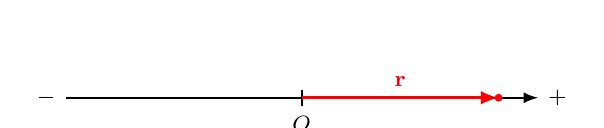
\begin{tikzpicture}
    \draw[axes] (-3,0)--(3,0) node[pos=0,left]{$-$} node[right]{$+$};
    %\foreach \x in {-5,...,5} \draw (\x,.1)--(\x,-.1);
    \draw[thick] (0,.1)--(0,-.1) node[below]{$O$};
    \fill[red] (2.5,0) circle (.05);% node[below]{$A$};
    \draw[vectors,red] (0,0)--(2.5,0) node[midway,above]{$\mathbf r$};
  \end{tikzpicture}
  \caption{Position in a one-dimensional coordinate system}
  \label{fig:1d-position}
\end{figure}

In a two-dimesional coordinate system (e.g.\ $xy$-plane),
%\textbf{Position in 2D Coordinate System:} For two-dimensional motion,
there are several ways to describe an object's position. One way is to use the
$x$ and $y$ coordinates. The positions of the object at $P$ and $Q$ are:
\begin{align*}
  \vec r_P & =3\hat x + 2\hat y\\
  \vec r_Q & =-4\hat x + 3\hat y
\end{align*}
or the length of the straight line from the origin to
the position, and the angle it makes with the $x$ axis.
\begin{figure}[ht]
  \centering
  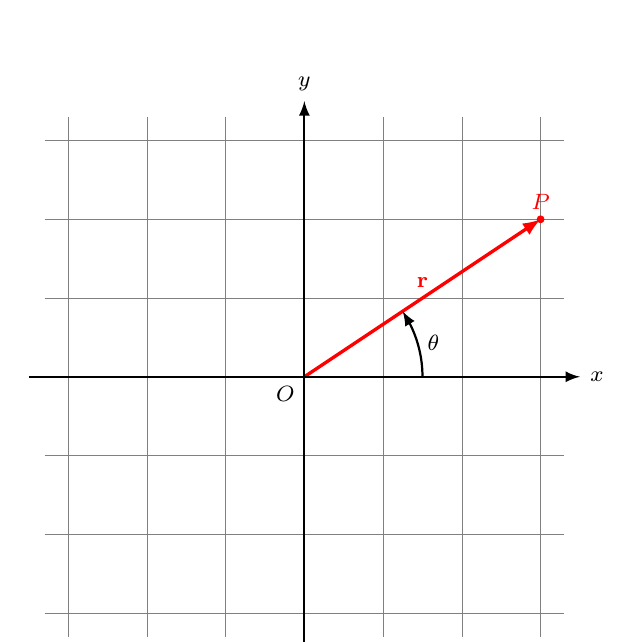
\begin{tikzpicture}
    \draw[help lines] (-3.3,-3.3) grid (3.3,3.3);
    \fill[red] (3,2) circle (.05) node[above]{$P$};
    \draw[vectors,red] (0,0)--(3,2) node[midway,above]{$\mathbf r$};
    \draw[axes] (-3.5,0)--(3.5,0) node[right]{$x$};
    \draw[axes] (0,-3.5)--(0,3.5) node[above]{$y$};
    \draw[axes] (1.5,0) arc (0:atan(2/3):1.5) node[midway,right]{$\theta$};
    \node[below left] at (0,0) {$O$};
  \end{tikzpicture}
  \caption{Position in a two-dimensional coordinate system}
\end{figure}



\subsection{Displacement}
\textbf{Displacement} ($\Delta\mathbf r$) is the \emph{change in position} when
an object moves through the coordinate system. Mathematically, displacement is
defined as the \emph{difference} between the initial position
$\mathbf r_1=\mathbf r(t_1)$ when motion begins, and the current position
$\mathbf r(t)$ of the object. Therefore, as the object moves, $\Delta\mathbf r$
is also a continuous function of time, i.e.:
%\begin{equation*}
%  \Delta\mathbf r=  \Delta\mathbf r(t)
%\end{equation*}
\begin{equation}
  \boxed{
    \Delta\mathbf r(t)=\mathbf r(t)-\mathbf r_1
  }
\end{equation}
Graphically, displacement is drawn as a vector pointing from the initial
position $\mathbf r_1$ towards the current/final position $\mathbf r$.
%\begin{figure}[ht]
%  \centering
%  \begin{tikzpicture}[scale=.5]
%    \draw[axes] (0,0)--(6,0) node[right]{$x$};
%    \draw[axes] (0,0)--(0,8) node[above]{$y$};
%    \draw[vectors,red] (0,0)--(4,1) node[midway,above]{$\mathbf r_1$};
%    \draw[vectors,red] (0,0)--(2,6) node[midway,left]{$\mathbf r_2$};
%    \draw[vectors,blue] (4,1)--(2,6) node[midway,right]{$\Delta\mathbf r$};
%  \end{tikzpicture}
%\end{figure}

\begin{figure}[ht]
  \centering
  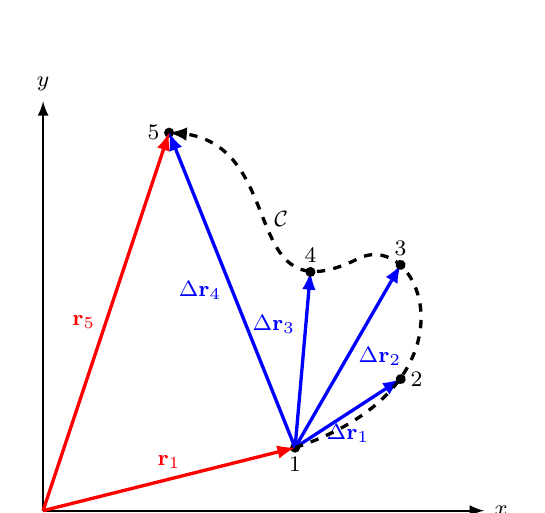
\begin{tikzpicture}[scale=.8]
    \draw[axes] (0,0)--(7,0) node[right]{$x$};
    \draw[axes] (0,0)--(0,6.5) node[above]{$y$};
    \fill (4,1) circle (.08) node[below]{1};
    \fill (2,6) circle (.08) node[left]{5};
    \draw[vectors,red] (0,0)--(4,1) node[midway,above]{$\mathbf r_1$};
    \draw[vectors,red] (0,0)--(2,6) node[midway,left] {$\mathbf r_5$};
    \begin{scope}[rotate around={33:(4,1)}]
      \draw[vector,blue] (4,1)--+(2,0) node[midway,below]{$\Delta\mathbf r_1$};
      \fill (6,1) circle (.08) node[right]{2};
    \end{scope}
    \begin{scope}[rotate around={60:(4,1)}]
      \draw[vector,blue] (4,1)--+(3.35,0) node[midway,right]{$\Delta\mathbf r_2$};
      \fill (7.35,1) circle (.08) node[above]{3};
    \end{scope}
    \begin{scope}[rotate around={85:(4,1)}]
      \draw[vector,blue] (4,1)--+(2.8,0) node[pos=.7,left=0]{$\Delta\mathbf r_3$};
      \fill (6.8,1) circle (.08) node[above]{4};
    \end{scope}
    \draw[vectors,blue] (4,1)--(2,6) node[midway,left]{$\Delta\mathbf r_4$};
    %\fill (7,2) circle (.07);
    %\fill (6,4.5) circle (.07);
    %\fill[cyan] (3,3) circle (.07);
    %\fill[cyan] (4,6) circle (.07);
    \draw[very thick,dashed,->] (4,1) ..controls (7,2) and (6,4.5).. (5,4)
    ..controls (3,3) and (4,6).. (2,6) node[midway,right]{$\mathcal C$};
  \end{tikzpicture}
  \caption{The displacement of an object evolves with time as it moves.}
\end{figure}


The SI unit for displacement is also \textbf{metre} (\si\metre).



\textbf{Explain why this is a subtraction}


\subsection{Distance}

\textbf{Distance} ($s$) is a quantity that is \emph{similar} to
displacement. It is the length of the path $\mathcal C$ taken as an object
moves from initial position ($\mathbf r_1$) to its current/final position
($\mathbf r(t)$). Unlike displacement, distance is a \emph{length}, and therefore
it is \emph{scalar} quantity. For the same reason, distance is non-negative
(i.e.\ $s\geq 0$). As the object moves, distance is always increasing. Since
the length changes with time, distance is also a continuous function of time:
\begin{equation*}
  \boxed{s=s(t)}
\end{equation*}
%\item Depends on \emph{how} the object travels from $\mathbf r_1$ to
%  $\mathbf r_2$
Although the magnitude of the displacement vector $|\Delta\mathbf r|$ is also a
scalar, it is \emph{not} necessarily the same as distance. In classical
physics,  $s\geq |\Delta\mathbf r|$

%\begin{figure}
%  \centering
%  \begin{tikzpicture}[scale=.5]
%    \draw[axes] (0,0)--(6,0) node[right]{$x$};
%    \draw[axes] (0,0)--(0,8) node[above]{$y$};
%    \draw[vectors,red] (0,0)--(4,1) node[midway,above]{$\mathbf r_1$};
%    \draw[vectors,red] (0,0)--(2,6) node[midway,left] {$\mathbf r_2$};
%    \draw[vectors,blue] (4,1)--(2,6) node[midway,right]{$\Delta\mathbf r$};
%    \draw[very thick,dash dot] (4,1)..controls (6,5) and (5,7)..(2,6)
%    node[midway,right]{$s$};
%  \end{tikzpicture}
%\end{figure}




\subsection{Velocity}

\textbf{Average velocity} ($\mathbf v_\text{avg}$) is how quickly your position
changes \emph{over a finite time interval}. It is a vector quantity with an
SI unit of \textbf{metres per second} (\si{\metre\per\second}). The direction
of $\mathbf v_\text{avg}$ is the same as displacement $\Delta\mathbf d$, and it is
also a function of time:
\begin{equation}
  \boxed{
    \mathbf v_\text{avg}(t)
    =\frac{\Delta\mathbf r(t)}{\Delta t}
    =\frac{\mathbf r(t)-\mathbf r_1}{t-t_1}
  }
\end{equation}
where $\mathbf r_1=\mathbf r(t_1)$ is the initial position at initial time $t_1$

In contrast, \textbf{instantaneous velocity} ($\mathbf v$) is how quickly
your displacement is changing \emph{at a specific instance in time}
\begin{itemize}
\item Obtained by letting the time interval \emph{infinitesimally} small,
  i.e.\ $\Delta t\rightarrow 0$
\item Also called the \emph{rate of change in displacement}
\item Calculating instantaneous velocity may require calculus\footnote{For
those of you who know a bit of calculus, the definition of instantenous
velocity is:
\begin{displaymath}
  \mathbf v(t)=\frac{d\mathbf r}{dt}
\end{displaymath}}  
\end{itemize}




\subsection{Speed}

\textbf{Average speed} ($v$) is similar to average velocity, but instead of
using displacement, it is the distance ($s$) travelled over a \emph{finite}
time interval. Speed is a \emph{scalar}:
  
\begin{equation}
  \boxed{
    v_\text{avg}(t)
    =\frac{s(t)}{\Delta t}\geq 0
  }
\end{equation}
Similarly, \textbf{instantaneous speed} ($v$) is how quickly
distance is changing at a \emph{specific instance} in time.
\begin{itemize}
\item Since distance is always positive ($s\ge 0$), both average and
  instantaneous speeds must always be positive
\end{itemize}




\subsection{Acceleration}

\textbf{Average acceleration} ($\mathbf a_\text{avg}$) is how quickly the
instantaneous velocity vector changes over a \emph{finite} time interval,
with an SI unit of \textbf{metres per second squared}
(\si{\metre\per\second\squared}):
\begin{equation}
  \boxed{\mathbf a_\text{avg}(t)
    =\frac{\Delta\mathbf v(t)}{\Delta t}
    =\frac{\mathbf v(t)-\mathbf v_1}{t-t_1}
  }
\end{equation}
where $\mathbf v_1=\mathbf v(t_1)$ is the initial velocity $\mathbf v$ at initial time
$t_1$.

\textbf{Instantaneous acceleration} ($\mathbf a(t)$) is how quickly the velocity
vector is changing at a \emph{specific instance} in time

A few things to note about acceleration:
\begin{itemize}
\item i.e.\ \emph{the rate of change of instantaneous velocity}
\item A change in a vector ($\Delta\mathbf v$) can mean a change in magnitude
  and/or direction
\item There can be acceleration without any speeding up or slowing down!
\item Think  about what happens if a car is turning at constant speed
\end{itemize}




%\section{Working with Vectors}
%  Vectors obey the \emph{principle of superposition}, which means that they
%  \emph{add} together. Methods for adding vectors include:
%  \begin{itemize}
%  \item Using \textbf{Pythagorean theorem} (for vectors at right angles to
%    each other)
%  \item Using \textbf{cosine and sine laws}
%  \item Decomposing vectors into \textbf{components}, then reassemble them
%    using Pythagorean theorem
%  \end{itemize}
%  For 1D problems, ($+$) and ($-$) signs are sufficient to indicate direction
%  \begin{itemize}
%  \item Remember to indicate which way is positive though!
%  \end{itemize}
%  \textbf{WARNING:} When adding vectors, you
%  \underline{\textbf{\emph{must not}}} simply add the magnitudes of the vectors!



%
%\section{Basic Motion Graphs}
%We can describe \emph{one-dimensional} motion graphically using
%\textbf{motion graphs}, by plotting
%\begin{itemize}
%\item Position vs.\ time ($d$--$t$)
%\item Instantaneous velocity vs.\ time ($v$--$t$)
%\item Instantaneous acceleration vs.\ time ($a$--$t$)
%\end{itemize}



\section{Basic Motion Graphs}
In one-dimension, motion can 
%  %the kinematic equations\footnote{They can only
%  %  be used for constant acceleration!} can
also be expressed graphically using \textbf{motion graphs}. The most basic
motion graphs are motion quantities as functions of time:
\begin{itemize}[itemsep=3pt]
\item Position vs.\ time ($r$ vs.\ $t$)
\item Instantaneous velocity vs.\ time ($v$ vs.\ $t$)
\item Instantaneous acceleration vs.\ time ($a$ vs.\ $t$)
\end{itemize}
At the moment, we are interested in:
\begin{itemize}[itemsep=3pt]
\item What the graphs themselves tell us
\item What the slopes of the graphs tell us
\item What the areas under the graphs tell us
\end{itemize}



\subsection{Position vs.\ Time Graph}
The \emph{most} obvious choice for expressing 1D motion of an object
graphically is by plotting its position as a function of time ($r(t)$). An
example is shown in Fig.~\ref{fig:pos-time-graph}.
\begin{figure}[ht]
  \centering
  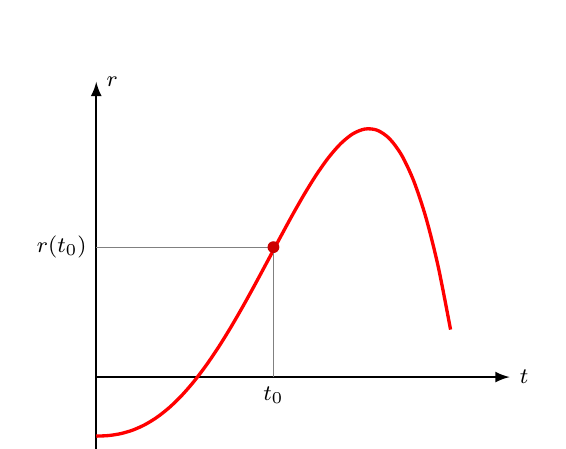
\begin{tikzpicture}[scale=1.5]
    \draw[axes] (0,0)--(3.5,0) node[right]{$t$};
    \draw[axes] (0,-.7)--(0,2.5) node[right]{$r$};
    \draw[functions,smooth,samples=30,domain=0:3]
    plot({\x},{-.2*\x^4+.5*\x^3+.4*\x^2-.5});
    
    \draw[gray] (1.5,0)--(1.5,1.1) node[pos=0,below,black]{$t_0$}
    --(0,1.1) node[left,black]{$r(t_0)$};
    \fill[red!80!black] (1.5,1.1) circle (.05);
  \end{tikzpicture}
  \caption{A typical position vs.\ time graph}
  \label{fig:pos-time-graph}
\end{figure}   
In a position vs.\ time graph, the horizontal ($x$) axis (independent variable)
is time $t$, while the the vertical ($y$) axis (dependent variable) is the
position $r$ measured from origin.
%\item Position in one-dimension can be $+/-$
%Generally, motion begins at $t=0$.
As shown in Figure~\ref{fig:pos-time-graph}, to find position at time $t_0$,
you can simply read the graph!
%\item Time only moves forward, but the graph does not explicitly tell you
%  so




\subsubsection{Slope of Secant: Average Velocity}
\textbf{Average velocity} of an object's motion is the
\emph{slope of the secant} of the position vs.\ time graph.
\begin{figure}[ht]
  \centering
  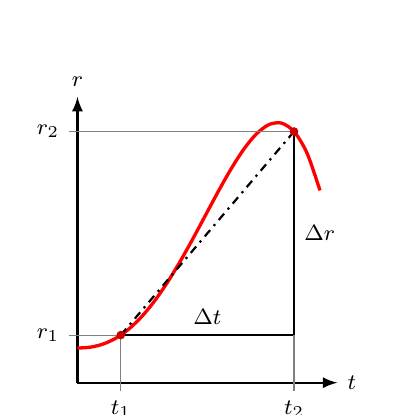
\begin{tikzpicture}[scale=1.1]
    \draw[axes] (0,0)--(0,3.3) node[above]{$r$};
    \draw[axes] (0,0)--(3,0) node[right]{$t$};
    \draw[functions,smooth,samples=20,domain=0:2.8]
    plot({\x},{-.2*\x^4+.5*\x^3+.4*\x^2+.4});
    \draw[thick,dash dot](.5,.55)--(2.5,2.9);
    \draw[thick] (.5,.55)--(2.5,.55)node[midway,above]{$\Delta t$}
    --(2.5,2.9) node[midway,right]{$\Delta r$};
    \draw[gray] (.5,.55)--(.5,-.1) node[below,black]{$t_1$};
    \draw[gray] (2.5,.55)--(2.5,-.1) node[below,black]{$t_2$};
    \draw[gray] (.5,.55)--(-.1,.55) node[left,black]{$r_1$};
    \draw[gray] (2.5,2.9)--(-.1,2.9) node[left,black]{$r_2$};
    \fill[red!80!black] (.5,.55) circle (.05);
    \fill[red!80!black] (2.5,2.9) circle (.05);
  \end{tikzpicture}
  \hspace{.1in}
  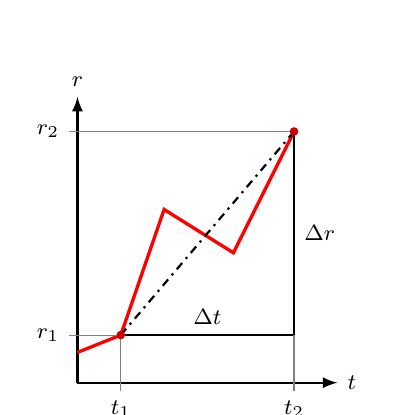
\begin{tikzpicture}[scale=1.1]
    \draw[axes] (0,0)--(0,3.3) node[above]{$r$};
    \draw[axes] (0,0)--(3,0) node[right]{$t$};
    \draw[functions] (0,.35)--(.5,.55)--(1,2)--(1.8,1.5)--(2.5,2.9);
    \draw[thick,dash dot] (.5,.55)--(2.5,2.9);
    \draw[thick] (.5,.55)--(2.5,.55)node[midway,above]{$\Delta t$}
    --(2.5,2.9) node[midway,right]{$\Delta r$};
    \draw[gray] (.5,.55)--(.5,-.1) node[below,black]{$t_1$};
    \draw[gray] (2.5,.55)--(2.5,-.1) node[below,black]{$t_2$};
    \draw[gray] (.5,.55)--(-.1,.55) node[left,black]{$r_1$};
    \draw[gray] (2.5,2.9)--(-.1,2.9) node[left,black]{$r_2$};
    \fill[red!80!black] (.5,.55) circle (.05);
    \fill[red!80!black] (2.5,2.9) circle (.05);
    \end{tikzpicture}
\end{figure}
%  \vspace{-.1in}Same average velocity in both graphs, but very different
%  motions
%  \begin{itemize}
%  \item ($+$) slope: motion in the ($+$) direction during the time interval
%  \item ($-$) slope: motion in the ($-$) direction during the time interval
%  \item Zero slope: no displacement over this time interval
%  \end{itemize}
%\end{frame}
%
%
%
\subsubsection{Instantaneous Velocity:} The instantaneous velocity of an object
is the \emph{slope of the tangent} to the curve of the position vs.\ time graph
at a specific time.
\begin{figure}[ht]
  \centering
  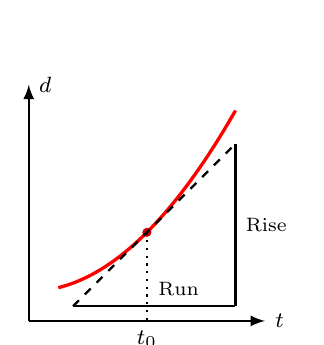
\begin{tikzpicture}[scale=.75]
    \draw[axes] (0,0)--(4,0) node[right] {$t$};
    \draw[axes] (0,0)--(0,4) node[right] {$d$};
    \draw[functions,smooth,samples=20,domain=.5:3.5]
    plot({\x},{.25*\x^2+.5});
    \fill[red!80!black] (2,1.5) circle (2.2pt);
    \draw[dotted,thick] (2,1.5)--(2,0) node[below] {$t_0$};
    
    \draw[smooth,samples=4,domain=.75:3.5,thick,dashed]
    plot({\x},{\x-.5});
    \draw[thick] (.75,.25)--(3.5,.25) node[pos=.65,above] {\scriptsize Run};
    \draw[thick] (3.5,.25)--(3.5,3) node[midway,right] {\scriptsize Rise};
    
  \end{tikzpicture}
\end{figure}

Like average velocity, the sign of the slope also indicates the direction of
motion. If position data is obtained experimentally, it may be difficult to
obtain an accurate value for instantaneous velocity.

%  What can we learn about instantaneous velocity from this position vs.\ time
%  graph?
%\begin{figure}
%  \begin{center}
%    \begin{tikzpicture}
%      \draw[axes] (0,0)--(3.5,0) node[right]{$t$};
%      \draw[axes] (0,-.7)--(0,2.5) node[right]{$d$};
%      \draw[functions,smooth,samples=30,domain=0:3]
%      plot({\x},{-.2*\x^4+.5*\x^3+.4*\x^2-.5});
%      \uncover<2->{
%        \begin{scope}[thick,cyan]
%          \draw (-.4,-.5)--+(.8,0) node[midway,below=-2]{$v=0$};
%          \draw (1.9,2.1)--+(.8,0) node[midway,above=-2]{$v=0$};
%          \draw (2.3,2.1)--(2.3,0) node[below=-2]{$t_1$};
%          \draw (0,-.5)--(0,0);
%        \end{scope}
%        \fill[cyan] (0,-.5) circle (.07);
%        \fill[cyan] (2.3,2.1) circle (.07);
%      %  \draw[dash dot,thick] (1.5,0)--(1.5,1.1) node[pos=0,below]{$t_0$}
%      %  --(0,1.1) node[left]{$d(t_0)$};
%      %  \fill[red!80!black] (1.5,1.1) circle (.05);
%      }
%      \uncover<3->{
%        \fill[pink!35,opacity=.3] (0,-.7) rectangle (2.3,2.3);
%        \draw[<-,thick,red] (.75,1) to[out=120,in=0] +(-1,.2)
%        node[left,text width=98,draw=red,fill=magenta!10]{\scriptsize
%          For $0<t<t_0$, velocity is positive ($v>0$) because the graph has a
%          positive slope\par};
%      }
%      \uncover<4->{
%        \fill[cyan!35,opacity=.3] (2.3,-.7) rectangle (3,2.3);
%        \draw[<-,thick,blue] (2.6,1) to[out=90,in=180] +(1.6,.4)
%        node[right,text width=86,draw=blue,fill=cyan!30]{\scriptsize
%          For $t>t_0$, velocity is negative ($v<0$) because the slope is
%          negative\par};
%      }
%    \end{tikzpicture}
%  \end{center}
%\end{frame}
%
%
%
%
\textbf{Acceleration:} Finding instantaneous acceleration $a(t)$ from a
position vs.\ time graph is \emph{very} difficult\footnote{If you already know
the function $r(t)$ exactly, then you can use calculus to find acceleration
exactly. In that case you don't really \emph{need} this graph in the first
place.}, but we can still find the \emph{sign} of acceleration based on whether
the graph opens up or down.
%In this example:
\begin{figure}[ht]
  \centering
  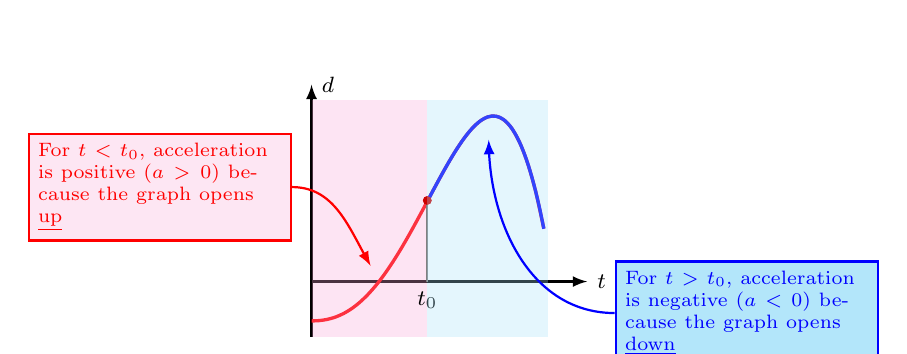
\begin{tikzpicture}
    \draw[axes] (0,0)--(3.5,0) node[right]{$t$};
    \draw[axes] (0,-.7)--(0,2.5) node[right]{$d$};
    \draw[functions,smooth,samples=30,domain=0:2.95]
    plot({\x},{-.2*\x^4+.5*\x^3+.4*\x^2-.5});
    %\uncover<2->{
      \fill[magenta!35,opacity=.3] (0,-.7) rectangle (1.47,2.3);
      \draw[<-,thick,red] (.75,.2) to[out=120,in=0] +(-1,1)
      node[left,text width=88,draw=red,fill=magenta!10]{\scriptsize
        For $t<t_0$, acceleration is positive ($a>0$) because the graph opens
        \underline{up}\par};
      \draw[thick,gray](1.47,1.03)--(1.47,0) node[below,black]{$t_0$};
      \fill[red!80!black] (1.47,1.03) circle (.055);
    %}
    %\uncover<3->{
      \draw[functions,smooth,samples=30,domain=1.48:2.95,blue]
      plot({\x},{-.2*\x^4+.5*\x^3+.4*\x^2-.5});
      \fill[red!80!black] (1.47,1.03) circle (.055);
      \fill[cyan!35,opacity=.3] (1.47,-.7) rectangle (3,2.3);
      \draw[<-,thick,blue] (2.25,1.8) to[out=270,in=180] +(1.6,-2.2)
      node[right,text width=88,draw=blue,fill=cyan!30]{\scriptsize
        For $t>t_0$, acceleration is negative ($a<0$) because the graph opens
        \underline{down}\par};
    %}
  \end{tikzpicture}
\end{figure}

%
%
%
\subsection{Velocity vs.\ Time Graph}

A less obvious choice for expressing 1D motion is by plotting
\emph{instantaneous} velocity as a function of time, i.e.\ $v=v(t)$. In
essence, we are plotting the slope of the position vs.\ time graph instead.
Using our example position vs.\ time graph:

\begin{figure}[ht]
  \centering
  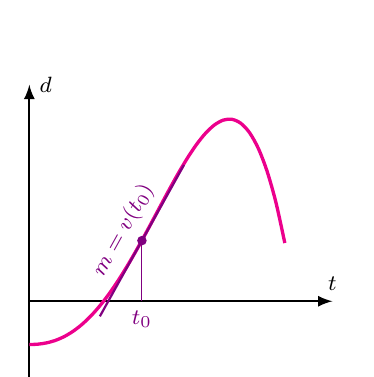
\begin{tikzpicture}[scale=1.1]
    \draw[axes] (0,0)--(3.5,0) node[above]{$t$};
    \draw[axes] (0,-1)--(0,2.5) node[right]{$d$};
    \draw[functions,smooth,samples=30,domain=0:2.95,magenta]
    plot(\x,{-.2*\x^4+.5*\x^3+.4*\x^2-.5});

    \fill[violet] (1.3,.7) circle (.055);
    \draw[violet] (1.3,.7)--(1.3,0) node[below]{$t_0$};
    \draw[thick,violet,rotate around={atan(1.8):(1.3,.7)}] (.3,.7)--+(2,0)
    node[midway,above,rotate=atan(1.8)]{$m=v(t_0)$};
  \end{tikzpicture}
  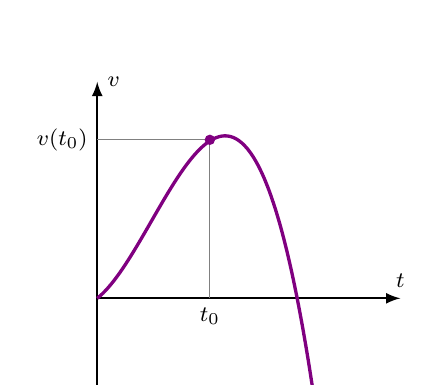
\begin{tikzpicture}[scale=1.1]
    \draw[axes] (0,0)--(3.5,0) node[above]{$t$};
    \draw[axes] (0,-1)--(0,2.5) node[right]{$v$};
    \draw[smooth,samples=40,domain=0:2.5,functions,violet]
    plot(\x,{-.8*\x^3+1.5*\x^2+.8*\x});
    \draw[gray] (1.3,0)--(1.3,1.83) node[pos=0,below,black]{$t_0$}
    --(0,1.83) node[left,black]{$v(t_0)$};
    \fill[violet] (1.3,1.83) circle (.06);
  \end{tikzpicture}

\end{figure}

%
%
%
%\begin{frame}{Velocity vs.\ Time Graph}
%%  \begin{columns}
%%    \column{.7\textwidth}
%%    \begin{itemize}
%  The velocity vs.\ time graph shows how instantaneous velocity evolves with
%  time. In this example:
%%    \item<3->Slope of the secant: average acceleration
%%    \item<3->Slope of the tangent: instantaneous acceleration
%%    \end{itemize}
%%    
%%    \column{.3\textwidth}
%  \begin{center}
%    \begin{tikzpicture}
%      \draw[axes] (0,0)--(3,0) node[right=-2]{$t$};
%      \draw[axes] (0,-1.5)--(0,2.2) node[above=-2]{$v$};
%      \draw[smooth,samples=45,domain=0:2.55,very thick,violet]
%      plot(\x,{-.8*\x^3+1.5*\x^2+.8*\x});
%      \uncover<2->{
%        \fill[violet] (2.3,0) circle (.055) node[below left=-2]{$t_1$};
%        \fill[violet] circle (.055) node[left=-2]{$0$};
%        \draw[<-,violet,thick] (-.4,0)--+(-3,0)
%        node[text width=80,draw=violet,fill=violet!10]{\scriptsize
%          At $t=0$ and $t=t_1$, velocity is zero ($v=0$)\par};
%      }
%      \uncover<3->{
%        \draw[gray] (1.47,1.87)--(1.47,0) node[below,violet]{$t_0$};
%        \fill[violet] (1.47,1.87) circle (.055);
%        \draw[<-,thick,violet] (1.55,1.87) to[out=30,in=150] +(1.6,0)
%        node[right,text width=75,draw=violet,fill=violet!10]{\scriptsize
%          At $t=t_0$, velocity is maximum. The slope is zero at this point.
%          \par};
%      }
%    \end{tikzpicture}
%  \end{center}
%  Velocity is positive when the graph is above the time axis; and negative
%  when below the time axis
%
%%    \begin{tikzpicture}[scale=1.1]
%%      \draw[axes] (0,0)--(3.5,0) node[above]{$t$};
%%      \draw[axes] (0,-1.25)--(0,2.75) node[right]{$v$};
%%      \draw[functions,smooth,samples=40,domain=0:3]
%%      plot({\x},{1.35*(\x-1)*(\x-1)-1.1*\x+.5});
%%      \uncover<2>{
%%        \draw[smooth,samples=40,domain=.626:2.189,orange,very thick]
%%        plot({\x},{1.35*(\x-1)*(\x-1)-1.1*\x+.5});
%%        \draw[smooth,samples=40,domain=2.189:3,violet,very thick]
%%        plot({\x},{1.35*(\x-1)*(\x-1)-1.1*\x+.5});
%%        \draw[smooth,samples=40,domain=0:.626,violet,very thick]
%%        plot({\x},{1.35*(\x-1)*(\x-1)-1.1*\x+.5});
%%      }
%%    \end{tikzpicture}
%%  \end{columns}
%\end{frame}
%
%

\textbf{Average Acceleration:}
%  \begin{center}
%    \begin{tikzpicture}[scale=1.1]
%      \draw[axes] (0,0)--(3,0) node[right=-2]{$t$};
%      \draw[axes] (0,-1.5)--(0,2.2) node[above=-2]{$v$};
%      \draw[smooth,samples=45,domain=0:2.55,very thick,violet]
%      plot(\x,{-.8*\x^3+1.5*\x^2+.8*\x});
%      %\uncover<2->{
%      %  \fill[violet] (2.3,0) circle (.055) node[below left=-2]{$t_1$};
%      %  \fill[violet] (0,0) circle (.055) node[left=-2]{$0$};
%      %}
%    \end{tikzpicture}
%  \end{center}
%\end{frame}
%
%
%
\textbf{Instantaneous Acceleration:}
%  \begin{center}
%    \begin{tikzpicture}[scale=1.1]
%      \draw[axes] (0,0)--(3,0) node[right=-2]{$t$};
%      \draw[axes] (0,-1.5)--(0,2.2) node[above=-2]{$v$};
%      \draw[smooth,samples=45,domain=0:2.55,very thick,violet]
%      plot(\x,{-.8*\x^3+1.5*\x^2+.8*\x});
%      %\uncover<2->{
%      %  \fill[violet] (2.3,0) circle (.055) node[below left=-2]{$t_1$};
%      %  \fill[violet] (0,0) circle (.055) node[left=-2]{$0$};
%      %}
%    \end{tikzpicture}
%  \end{center}



\textbf{Displacement and position:} The area under the velocity vs.\ time graph
is the \emph{displacement} of the object. In example below, the shaded area is
the displacement between $t_1$ and $t_2$. If the position at $t_1$ (i.e.\
$d_1$) is also known, then we can find the position at $t_2$ (i.e.\
$d_2=d_1+\Delta d$).
\begin{figure}[ht]
  \centering
  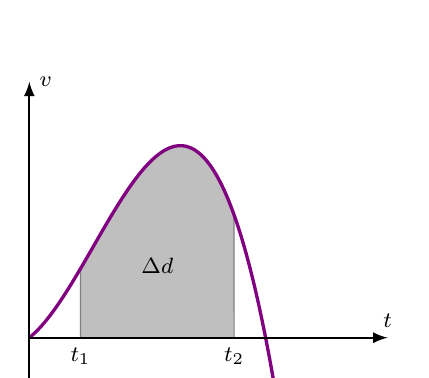
\begin{tikzpicture}[scale=1.3]
    \draw[smooth,samples=30,domain=.5:2,gray,fill=lightgray]
    plot(\x,{-.8*\x^3+1.5*\x^2+.8*\x})--(2,0) node[below,black]{$t_2$}
    --(.5,0) node[below,black]{$t_1$}--cycle;

    \draw[smooth,samples=50,domain=0:2.4,functions,violet]
    plot(\x,{-.8*\x^3+1.5*\x^2+.8*\x});

    \draw[axes] (0,0)--(3.5,0) node[above]{$t$};
    \draw[axes] (0,-.5)--(0,2.5) node[right]{$v$};

    \node at (1.25,.7) {$\Delta d$};
  \end{tikzpicture}
  \caption{The area under the velocity vs.\ time graph between $t_1$ and $t_2$
    gives us the object's displacement during this time interval.}
  \label{fig:area-under-vt-graph}
\end{figure}
If the area is \emph{above} the $x$-axis (time axis), then displacement
is positive ($\Delta d>0$); if the area is \emph{below} the $x$-axis, then
displacement is negative ($\Delta d<0$).



\subsection{Acceleration vs. Time Graph}
In the same way that we convert a position vs.\ time graph to a velocity vs.\
time graph, we can also convert a velocity vs.\ time graph to an
\textbf{acceleration vs.\ time} graph, by plotting the slope of the tangent.
This graph shows how \emph{instantaneous} acceleration $a(t)$ evolves with
time. In the example below:
%    \centering
%    \begin{tikzpicture}[scale=1.1]
%      \draw[axes] (0,0)--(3,0) node[right]{$t$};
%      \draw[axes] (0,-1)--(0,2.5) node[right]{$v$};
%      \draw[smooth,samples=40,domain=0:2.4,functions,violet]
%      plot(\x,{-.8*\x^3+1.5*\x^2+.8*\x});
%      %\fill[violet] (1.3,.7) circle (.06);
%      %\draw[violet] (1.3,.7)--(1.3,0) node[below]{$t_0$};
%    \end{tikzpicture}
%    
%    \column{.3\textwidth}
%    \centering
%    \begin{tikzpicture}[scale=1.1]
%      \draw[axes] (0,0)--(3,0) node[right]{$t$};
%      \draw[axes] (0,-2.3)--(0,1.2) node[right]{$a$};
%      \draw[smooth,samples=40,domain=0:2.2,functions,orange]
%      plot(\x,{-1.2*\x^2+1.5*\x+.4});
%      %\draw[gray] (1.3,0)--(1.3,1.83) node[pos=0,below,black]{$t_0$}
%      %--(0,1.83) node[left,black]{$v(t_0)$};
%      %\fill[violet] (1.3,1.83) circle (.06);
%    \end{tikzpicture}
%  \end{columns}

%\begin{frame}{Acceleration vs.\ Time Graph}

%  \begin{center}
%    \begin{tikzpicture}[scale=1.1]
%      \draw[axes] (0,0)--(2.8,0) node[right=-2]{$t$};
%      \draw[axes] (0,-2)--(0,1.2) node[right=-2]{$a$};
%      \draw[smooth,samples=40,domain=0:2.2,functions,orange]
%      plot(\x,{-1.2*\x^2+1.5*\x+.4});
%      \uncover<2->{
%        \fill[pink!40,opacity=.4] (0,-2) rectangle (1.48,1);
%        \fill[orange] (0.63,.87) circle (.06);
%        \draw[gray] (.63,0)--(.63,.87) node[pos=0,below=-2,black]{$t_0$}
%        --(0,.87) node[left=-2,black]{$a_\text{max}$};
%        \fill[orange] (1.48,0) circle (.06) node[above,black]{$t_1$};
%        \draw[thick,magenta,<-] (.75,-1)--+(-1,0)
%        node[left,text width=80,draw=magenta]{\scriptsize
%          Acceleration is positive from $t=0\rightarrow t_1$, with a maximum
%          magnitude of $a_\text{max}$ at $t_0$\par};
%      }
%      \uncover<3->{
%        \fill[violet] (1.48,0) circle (.06) node[above]{$t_1$};
%        \draw[thick,violet,<-] (1.48,.4) to[out=90,in=180] (3,1)
%        node[right,text width=70,draw=violet,fill=violet!10]{\scriptsize
%          Acceleration is zero ($a=0$) at $t=t_1$\par};
%      }
%      \uncover<4->{
%        \fill[cyan!40,opacity=.4] (1.48,-2) rectangle (2.4,1);
%        \draw[thick,blue,<-] (2.1,-.8)--+(1,0)
%        node[right,text width=63,draw=blue,fill=cyan!10]{\scriptsize
%          Acceleration is negative for $t>t_1$\par};
%      }
%    \end{tikzpicture}
%  \end{center}
%  \uncover<4->{
%    \vspace{-.1in}Remember: Since acceleration is a vector, \emph{positive}
%    acceleration means acceleration \emph{in the positive
%    \underline{direction}}, but it does not necessarily mean the object speeds
%    up
%  }
%\end{frame}
%
%

\subsubsection{Slope of the Acceleration vs.\ Time Graph}
The slope of the acceleration vs.\ time graph is the rate of change of
acceleration, called \textbf{jerk}.\footnote{The slope of the tangent is
called \textbf{instantaneous jerk}, whereas the slope of the secant is the
\textbf{average jerk}.}. This is \emph{not} a topic that is covered in Grade
11 or 12 Physics.
\begin{figure}[ht]
  \centering
  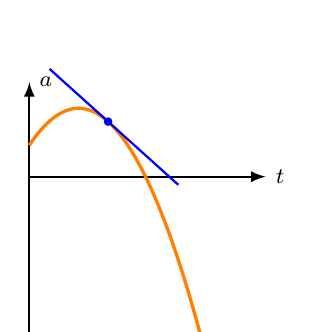
\begin{tikzpicture}
    \draw[axes] (0,0)--(3,0) node[right]{$t$};
    \draw[axes] (0,-2)--(0,1.2) node[right]{$a$};
    \draw[smooth,samples=40,domain=0:2.2,functions,orange]
    plot(\x,{-1.2*\x^2+1.5*\x+.4});
    \fill[blue] (1,.7) circle (.055);
    \draw[blue,thick,rotate around={-atan(.9):(1,.7)}] (0,.7)--+(2.2,0);
  \end{tikzpicture}
\end{figure}



%\begin{frame}{Area Under the Acceleration vs.\ Time Graph}
%  The area under acceleration vs.\ time graph is the \emph{change in velocity}
%  $\Delta v$.
%  \begin{center}
%    \begin{tikzpicture}
%      \draw[axes] (0,0)--(3,0) node[right]{$t$};
%      \draw[axes] (0,-2)--(0,1.2) node[right]{$a$};
%      \draw[smooth,samples=40,domain=0:2.2,functions,orange]
%      plot(\x,{-1.2*\x^2+1.5*\x+.4});
%      \uncover<2->{
%        \draw[smooth,samples=40,domain=.3:1.3,thick,gray,fill=lightgray!50]
%        plot(\x,{-1.2*\x^2+1.5*\x+.4})--(1.3,0) node[below=-2,black]{$t_2$}
%        --(.3,0) node[below=-2,black]{$t_1$}--cycle;
%        \draw[thick,<-,black!80] (.8,.3)--+(-1.5,0)
%        node[text width=72,left,draw=black!80,fill=lightgray!50]{\scriptsize
%          $\Delta v>0$ from $t_1\rightarrow t_2$ because the area is above the
%          $x$ axis\par};
%      }
%      \uncover<3->{
%        \draw[smooth,samples=40,domain=1.7:2.1,thick,cyan,fill=cyan!20]
%        plot(\x,{-1.2*\x^2+1.5*\x+.4})--(2.1,0) node[above=-2]{$t_4$}
%        --(1.7,0) node[above=-2]{$t_3$}--cycle;
%        \draw[thick,<-,blue] (1.9,-.5)--+(2,0)
%        node[text width=75,right,draw=blue,fill=cyan!20]{\scriptsize
%          $\Delta v<0$ from $t_3\rightarrow t_4$ because the area is below the
%          $x$ axis\par};
%      }
%    \end{tikzpicture}
%  \end{center}
%  \begin{itemize}
%  \item If the area is \emph{above} the $x$-axis (time axis), then $\Delta v>0$
%  \item If the area is \emph{below} the $x$-axis, then $\Delta v<0$
%  \item Remember: $\Delta v>0$ does not necessarily mean that the object
%    speeds up; $\Delta v<0$ does not necessarily mean that it will slow down
%  \end{itemize}
%\end{frame}


\section{Uniform Motion}
\textbf{Uniform motion} is when the velocity vector is constant, and neither
its magnitude nor direction changes. In 1D, the motion graphs look like this:
\vspace{-.1in}\begin{center}
  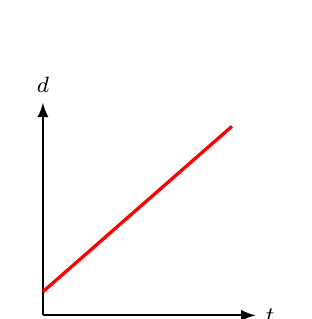
\begin{tikzpicture}[scale=.6]
    \draw[axes] (0,0)--(4.5,0) node[right]{$t$};
    \draw[axes] (0,0)--(0,4.5) node[above]{$d$};
    \draw[functions] (0,.5)--(4,4);
  \end{tikzpicture}
  \hspace{.15in}
  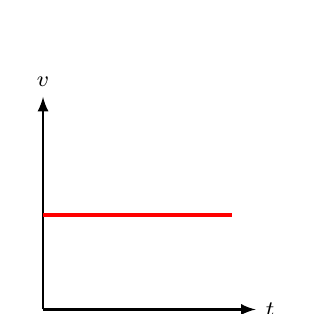
\begin{tikzpicture}[scale=.6]
    \draw[axes] (0,0)--(4.5,0) node[right]{$t$};
    \draw[axes] (0,0)--(0,4.5) node[above]{$v$};
    \draw[functions] (0,2)--(4,2);
  \end{tikzpicture}
  \hspace{.15in}
  \begin{tikzpicture}[scale=.6]
    \draw[axes] (0,0)--(4.5,0) node[right]{$t$};
    \draw[axes] (0,0)--(0,4.5) node[above]{$a$};
    \draw[functions] (0,0)--(4,0);
  \end{tikzpicture}
\end{center}
\begin{itemize}
\item \vspace{-.15in}$d$--$t$ graph is a straight line
\item The slope of the $d$--$t$ graph, which is velocity $v$, is also constant
\item There is no acceleration, so $a=0$ for all $t$
\end{itemize}




\section{Uniform Acceleration}
When a constant net force acts on an object, it moves with a constant
non-zero acceleration, or \textbf{uniform acceleration}.
\begin{center}
  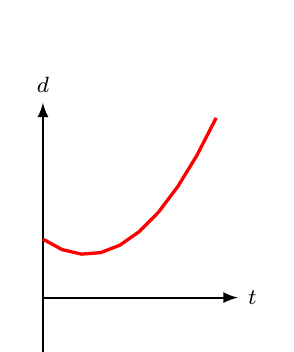
\begin{tikzpicture}[scale=.55]
    \draw[axes] (0,0)--(4.5,0) node[right]{$t$};
    \draw[axes] (0,-1.5)--(0,4.5) node[above]{$d$};
    \draw[functions,samples=10,domain=0:4] plot(\x,{.35*(\x-1)*(\x-1)+1});
  \end{tikzpicture}
  \hspace{.15in}
  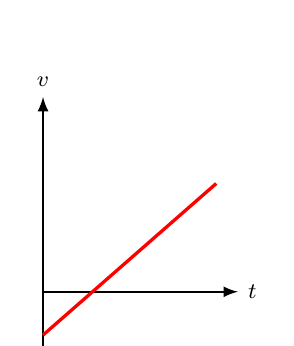
\begin{tikzpicture}[scale=.55]
    \draw[axes] (0,0)--(4.5,0) node[right]{$t$};
    \draw[axes] (0,-1.5)--(0,4.5) node[above]{$v$};
    \draw[functions] (0,-1)--(4,2.5);
  \end{tikzpicture}
  \hspace{.15in}
  \begin{tikzpicture}[scale=.55]
    \draw[axes] (0,0)--(4.5,0) node[right]{$t$};
    \draw[axes] (0,-1.5)--(0,4.5) node[above]{$a$};
    \draw[functions] (0,1)--(4,1);
  \end{tikzpicture}
\end{center}
\begin{itemize}
\item The $d$ vs.\ $t$ graph is part of a \emph{parabola}
  \begin{itemize}
  \item opens \emph{up}, then acceleration is positive
  \item opens \emph{down}, then acceleration is negative
  \end{itemize}
\item The $v$ vs.\ $t$ graph is a straight line; the (constant) slope is the
  cceleration
\end{itemize}




\section{Area Under Motion Graphs}
\begin{center}
  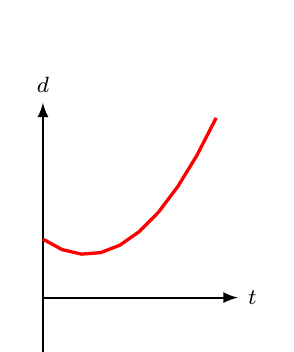
\begin{tikzpicture}[scale=.55]
    \draw[axes] (0,0)--(4.5,0) node[right]{$t$};
    \draw[axes] (0,-1.5)--(0,4.5) node[above]{$d$};
    \draw[functions,samples=10,domain=0:4] plot(\x,{.35*(\x-1)*(\x-1)+1});
  \end{tikzpicture}
  \hspace{.15in}
  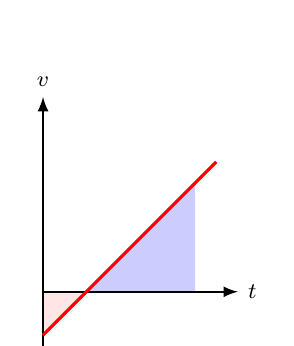
\begin{tikzpicture}[scale=.55]
    \draw[pink!40,fill=pink!40] (0,0)--(0,-1)--(1,0)--cycle;
    \draw[blue!20,fill=blue!20] (1,0)--(3.5,0)--(3.5,2.5)--cycle;
    \draw[axes] (0,0)--(4.5,0) node[right]{$t$};
    \draw[axes] (0,-1.5)--(0,4.5) node[above]{$v$};
    \draw[functions] (0,-1)--(4,3);
  \end{tikzpicture}
  \hspace{.15in}
  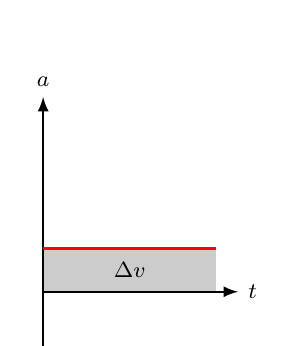
\begin{tikzpicture}[scale=.55]
    \fill[gray!40] rectangle (4,1) node[black,midway]{$\Delta v$};
    \draw[axes] (0,0)--(4.5,0) node[right]{$t$};
    \draw[axes] (0,-1.5)--(0,4.5) node[above]{$a$};
    \draw[functions] (0,1)--(4,1);
  \end{tikzpicture}
\end{center}
\begin{itemize}
\item The area under the $a$--$t$ graph is the change in velocity $\Delta v$
  \begin{itemize}
  \item If initial velocity is known, then we can plot $v$--$t$ graph based on
    this graph
  \end{itemize}
\item The area under the $v$--$t$ graph is the displacement $\Delta d$
  \begin{itemize}
  \item If the area is {\color{red!40}below} the $x$-axis (time axis), then
    displacement is negative;
  \item If the area is {\color{blue!20}above} the time axis, then
    displacement is positive
  \end{itemize}
\item The area under the $d$--$t$ graph has no physical meaning
\end{itemize}




\section{Simple Harmonic Motion}
In \textbf{simple harmonic motion}\footnote{Or \textbf{oscillatory motion},
or \textbf{vibration}}, displacement, velocity and acceleration are all
periodic functions, and none of them are constant!
\vspace{-.1in}
\begin{center}
  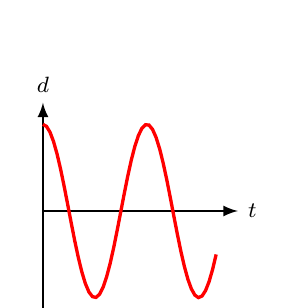
\begin{tikzpicture}[scale=.55]
    \draw[axes] (0,0)--(4.5,0) node[right]{$t$};
    \draw[axes] (0,-2.5)--(0,2.5) node[above]{$d$};
    \draw[functions,samples=50,domain=0:4] plot(\x,{2*cos(150*\x)});
  \end{tikzpicture}
  \hspace{.15in}
  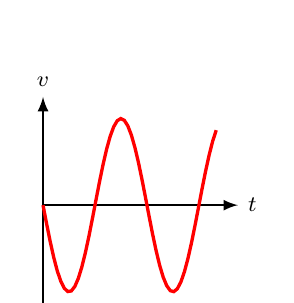
\begin{tikzpicture}[scale=.55]
    \draw[axes] (0,0)--(4.5,0) node[right]{$t$};
    \draw[axes] (0,-2.5)--(0,2.5) node[above]{$v$};
    \draw[functions,samples=50,domain=0:4] plot(\x,{-2*sin(150*\x)});
  \end{tikzpicture}
  \hspace{.15in}
  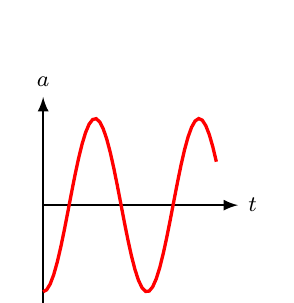
\begin{tikzpicture}[scale=.55]
    \draw[axes] (0,0)--(4.5,0) node[right]{$t$};
    \draw[axes] (0,-2.5)--(0,2.5) node[above]{$a$};
    \draw[functions,samples=50,domain=0:4] plot(\x,{-2*cos(150*\x)});
  \end{tikzpicture}
\end{center}
We will discuss this topic later, in the next unit.



%\section{Example Problem}
%  \textbf{Example:} Expression the motion in a \emph{position-time}
%  graph and an \emph{acceleration-time} graph. Assume the object's initial
%  position is the origin of the coordinate system.
%  \begin{center}
%    \begin{tikzpicture}[scale=.75]
%      \draw[help lines] grid (12,4);
%      \draw[axes] (0,0)--(13,0) node[right]{$t$ (\si\second)};
%      \foreach \t in {0,...,12} {
%        \draw(\t,0)--(\t,-.15) node[below]{$\t$};
%      }
%      \draw[axes] (0,0)--(0,5) node[above]{$v$ (\si{\metre\per\second})};
%      \foreach \v in {0,...,4} {
%        \draw(0,\v,0)--(-.15,\v) node[left]{$\v$};
%      }
%      \draw[functions] (0,2)--(2.5,2)--(5,4)--(7.5,4)--(10,1)--(12,1);
%    \end{tikzpicture}
%  \end{center}
%
%
%
%
\section{1D Kinematic Equations}

\begin{align*}
  \Delta d &=v_1\Delta t + \frac12a\Delta t^2\\
  \Delta d &=v_2\Delta t - \frac12a\Delta t^2\\
  \Delta d &=\frac{v_1+v_2}2 \Delta t\\
  v_2 &= v_1+ a \Delta t\\
  v_2^2 &= v_1^2+ 2a \Delta d
\end{align*}

There are five motion quantities of interest:
\begin{center}
  \begin{tabular}{l|c|c}
    \rowcolor{pink}
    \textbf{Quantity} & \textbf{Symbol} & \textbf{SI Unit} \\ \hline
    Displacement & $\Delta d$ & \si{\metre} \\
    Initial (instantaneous) velocity & $v_1$ & \si{\metre\per\second} \\
    Final (instantaneous) velocity   & $v_2$ & \si{\metre\per\second} \\
    Acceleration (constant) & $a$    & \si{\metre\per\second\squared}\\
    Time interval & $\Delta t$ & \si\second
  \end{tabular}
\end{center}
Only valid for \underline{\textbf{constant acceleration}}



%\section{1D Kinematic Equations}
%  \begin{columns}
%    \column{.35\textwidth}
%    {\large
%      \begin{align*}
%        \Delta d &=v_1\Delta t + \frac12a\Delta t^2\\
%        \Delta d &=v_2\Delta t - \frac12a\Delta t^2\\
%        \Delta d &=\frac{v_1+v_2}2 \Delta t\\
%        v_2 &= v_1+ a \Delta t\\
%        v_2^2 &= v_1^2+ 2a \Delta d
%      \end{align*}
%    }
%    \column{.65\textwidth}
\begin{itemize}
\item For 1-object problems, you are usually given 3 of the 5 variables,
  and you are asked to find a 4th one
\item For 2-object problems, the motion of the two objects are connected by
  time interval $\Delta t$ and displacement $\Delta d$
\item For 2D or 3D problems, each direction should have its own kinematic
  equations
\end{itemize}



%\section{1D Kinematic Equations}
Kinematic equations \emph{cannot} be used when acceleration is non-uniform
(when non-constant forces act on an object):
\begin{itemize}
\item Aerodynamic forces
  \begin{itemize}
  \item Lift and drag forces
  \item proportional to $v^2$
  \end{itemize}
\item Spring force
  \begin{itemize}
  \item The force that a compressed/stretched spring applies to connected
    objects
  \item Proportional to spring displacement $\mathbf x$
  \end{itemize}
\item Dampers in springs
  \begin{itemize}
  \item Dampers are used to slow down the vibration of an object
  \item Generally proportional to $v$
  \end{itemize}
\end{itemize}  
%We will discuss more about forces later in this unit.




%\section{Relative Motion}
%  \begin{center}
%    \vspace{-.15in}
%    \pic{.65}{graphics/57}
%  \end{center}
%  \begin{itemize}
%  \item Observers (frames of reference) A and B measures different motion of the
%    ball because A and B a moving relative to each other
%  \item The instantaneous velocity of the ball at any time $t$, as measured by
%    A and B, is related by the instantaneous velocities of A and B relative to
%    each other
%  \end{itemize}
%
%
%
%
%\section{Relative Motion}
%  All velocities are measured \emph{relative} to a frame of reference.
%  Therefore, when expressing relative motion, we can use two subscripts:
%    
%  \eq{-.15in}{
%    \mathbf v_{AB}
%  }
%    
%  \vspace{-.15in}where $A$ represents the object, and $B$ represents the frame
%  of reference
%
%  \vspace{.25in}\textbf{Example:} the velocity of an airplane ($P$) travelling
%  at \SI{251}{\kilo\metre\per\hour} [N] relative to Earth ($E$) is expressed as:
%
%  \eq{-.2in}{
%    \mathbf v_{PE}=\SI{251}{\kilo\metre\per\hour}\text{ [N]}
%  }
%
%
%
%
%\section{Relative Motion}
%  \begin{itemize}
%  \item Different observers make different observations because they (their
%    frames of reference) are moving relative to each other.
%  \item In \emph{classical} mechanics, the different velocity measurements are
%    related by the \textbf{Galilean velocity addition rule}\footnote{This
%    equation was thought to be so obvious that no one bothered to give it a
%    name until Einstein showed that it is not valid near the speed of light}:
%    
%    \eq{-.1in}{
%      \boxed{\mathbf v_{AC}=\mathbf v_{AB}+\mathbf v_{BC}}
%    }
%
%    \vspace{-.1in}The velocity of $A$ relative to reference frame $C$ is the
%    velocity of $A$ relative to reference frame $B$, plus the velocity of $B$
%    relative to $C$.
%  \item Can only be used when velocity $v$ is small compared to the speed of
%    light $c$
%  \end{itemize}
%
%
%%\section{Relative Motion}
%%  If we add another reference frame ($D$), the equation becomes:
%%
%%  \eq{-.3in}{
%%    \mathbf v_{AD}=\mathbf v_{AB}+\mathbf v_{BC}+\mathbf v_{CD}
%%  }
%%
%
%
%
%\section{Relative Motion Example: Airplane in Air}
%  The velocity of the plane relative to the ground (``ground speed'') is
%  the velocity of the plane relative to the air (``air speed'') plus
%  the velocity of the air relative to the ground (``wind speed'').  
%  \begin{center}
%    \pic{.4}{graphics/Planewind}
%  \end{center}
%  The addition of velocities is exactly the same as any vector addition.

%\section{Projectile Motion}
%  A \textbf{projectile} is an object that is launched with an initial velocity
%  of $\mathbf v_1$ along a parabolic trajectory and accelerates only due to
%  gravity.
%  \begin{columns}[T]
%    \column{.3\textwidth}
%    \begin{tikzpicture}[scale=1.6]
%      \draw[axes] (0,0)--(2,0) node[right]{$x$};
%      \draw[axes] (0,0)--(0,2) node[above]{$y$};
%      \draw[dotted,domain=0:2.7,thick] plot (\x, {1.2*\x-.2*\x*\x});
%      \draw[vectors] (0,0)--(.75,.9) node[above]{$\mathbf v_1$};
%      \draw[vectors,red] (0,0)--(0,.9) node[midway,left]{$v_y$};
%      \draw[vectors,blue] (0,0)--(.75,0) node[midway,below]{$v_x$};
%      \draw[axes] (.5,0) arc (0:52:.5) node[pos=.6,right]{$\theta$};
%    \end{tikzpicture}
%
%    \column{.67\textwidth}
%    \begin{itemize}
%    \item $x$-axis: \emph{horizontal}, pointing \emph{forward}
%    \item $y$-axis: \emph{vertical}, pointing \emph{up}
%    \item Angle $\theta$ measured \emph{above} the horizontal (i.e.\ $\theta>0$
%      when thrown upwards; $\theta<0$ then thrown downwards)
%    \item The origin is usually where the projectile is launched
%    \end{itemize}
%  \end{columns}
%
%
%
%
%\section{Horizontal Direction}
%  The initial velocity $\mathbf v_1$ can be decomposed into its $x$ and $y$
%  components:
%
%  \vspace{-.25in}{\large
%    \begin{align*}
%      v_x &=v_1\cos\theta \\
%      v_y &=v_1\sin\theta
%      \end{align*}
%  }
%
%  There is no horizontal acceleration (i.e.\ $a_x=0$), therefore $v_x$ is
%  constant. The kinematic equations reduce to a single equation:
%
%  \eq{-.1in}{
%    \Delta x=v_x\Delta t=\left[v_0\cos\theta\right]\Delta t
%  }
%
%  \vspace{-.1in}where $\Delta x$ is the horizontal displacement.
%
%
%
%
%
%\section{Vertical Direction}
%  There is constant vertical acceleration due to gravity alone, i.e.\
%  $a_y=-g$. ($a_y$ is \emph{negative} due to the way we defined the
%  coordinate system, with the $y$-axis pointing up.) The most important
%  kinetic equation is this one:
%
%  \eq{-.1in}{
%    \Delta y = \left[v_1\sin\theta\right]\Delta t-\frac12g\Delta t^2
%  }
%
%  These two kinematic equations may also be useful:
%
%  \vspace{-.25in}{\large
%    \begin{align*}
%      v_y &= \left[v_1\sin\theta\right] -gt\\
%      v_y^2&=\left[v_1^2\sin^2\theta\right]-2g\Delta y
%    \end{align*}
%  }
%
%
%
%
%\section{Solving Projectile Motion Problems}
%  Horizontal and vertical motions are linearly independent, but variables are
%  shared in both directions:
%  \begin{itemize}
%  \item Time interval $\Delta t$
%  \item Launch angle $\theta$ (above the horizontal)
%  \item Initial speed $v_1$
%  \end{itemize}
%  
%  \vspace{.25in}When solving any projectile motion problems
%  \begin{itemize}
%  \item \emph{Two} equations with \emph{two} unknowns
%  \item If an object lands on an incline, there will be a third equation
%    relating $x$ and $y$
%  \end{itemize}
%
%
%
%
%\section{Symmetric Trajectory}
%  A projectile's trajectory is \emph{symmetric} if the object lands at the same
%  height as when it launched. The angle $\theta$ is measured above the
%  horizontal. The \textbf{time of flight} ($T$), \textbf{range} ($R$)
%  and \textbf{maximum height} ($H$) are, respectively,
%
%  \eq{-.1in}{
%    \boxed{T=\frac{2v_1\sin\theta}g}\quad\quad
%    \boxed{R=\frac{v_1^2\sin(2\theta)}g}\quad\quad
%    \boxed{H=\frac{v_1^2\sin^2\theta}{2g}}
%  }
%
%
%
%
%\section{Maximum Range}
%  \eq{-.1in}{
%    R=\frac{v_1^2\sin(2\theta)}g
%  }
%  
%  \begin{itemize}
%  \item Maximum range occurs at $\theta=\ang{45}$
%  \item For a given initial speed $v_0$ and range $R$, launch angle $\theta$ is
%    given by:
%    
%    \eq{-.1in}{
%      \theta_1=\frac12\sin^{-1}\left(\frac{Rg}{v_1^2}\right)
%    }
%
%  \item But there is another angle that \emph{gives the same range}!
%
%    \eq{-.1in}{
%      \theta_2=\ang{90}-\theta_1
%    }
%  \end{itemize}
%
%%
%%
%%\section{Projectile Motion}
%%  \begin{itemize}
%%  \item For projectile motion problems, resolve the problem into horizontal
%%    ($x$) and vertical ($y$) directions, and apply kinematic equations
%%    independently
%%  \item No horizontal acceleration ($a_x=0$), therefore kinematic equations
%%    reduce to a single equation:
%%    
%%    \eq{-.3in}{\Delta x=v_x\Delta t}
%%  \item Acceleration due to gravity only in the vertical ($y$) direction:
%%    
%%    \eq{-.25in}{\mathbf a_y=\mathbf g=\magdir{\SI{9.81}{\metre\per\second^2}}{down}}
%%
%%    \vspace{-.15in}We \emph{usually} define the (+) direction to be [up], so
%%    $a_y=-g=\SI{-9.81}{\metre\per\second^2}$ %, but it can change depending on
%%    %the problem
%%  \end{itemize}
%%
%%
%%
%%\section{Solving Projectile Motion Problems}
%%  \begin{itemize}
%%  \item There are variables the two directions
%%    \begin{itemize}
%%    \item Initial speed $v_i$
%%    \item Angle above the horizontal $\theta$ (appears in the initial velocities
%%      in both horizontal and vertical directions)
%%    \item Time of motion $\Delta t$
%%    \end{itemize}
%%  \item Have two equations with two unknowns
%%  \item In more difficult problems, $\Delta y$ and $\Delta x$ can be related
%%    geometrically, (so $3$ equations with $3$ unknowns)
%%  \end{itemize}
%%
%%
%%
%%
\begin{example}
  While hiking in the wilderness, you come to a cliff
  overlooking a river. A topographical map shows that the cliff is
  \SI{291}{\metre} high and the river is \SI{68.5}{\metre} wide at that
  point. You throw a rock directly forward from the top of the cliff, giving
  the rock a horizontal velocity of \SI{12.8}{\metre\per\second}.
  \begin{enumerate}
  \item Did the rock make it across the river?
  \item With what velocity did the rock hit the ground or water?
  \end{enumerate}
  
  \begin{center}
    \pic{.5}{kinematics/graphics/cliff}
  \end{center}
\end{example}



\begin{example}
  A golfer hits the golf ball off the tee, giving it an
  initial velocity of \SI{32.6}{\metre\per\second} at an angle of \ang{65} with
  the horizontal. The green where the golf ball lands is \SI{6.30}{\metre}
  higher than the tee, as shown in the illustration. Find the time interval
  when the golf ball was in the air, and the distance to the green.
  \begin{center}
    \pic{.5}{kinematics/graphics/golfer}
  \end{center}
\end{example}



\begin{example}
  You are playing tennis with a friend on tennis courts
  that are surrounded by a \SI{4.8}{\metre} fence. You opponent hits the ball
  over the fence and you offer to retrieve it. You find the ball at a distance
  of \SI{12.4}{\metre} on the other side of the fence. You throw the ball at an
  angle of \ang{55.} with the horizontal, giving it an initial velocity of
  \SI{12.1}{\metre\per\second}. The ball is \SI{1.05}{\metre} above the ground
  when you release it. Did the ball go over the fence, hit the fence, or hit
  the ground before it reached the fence?
\end{example}



%\section{Symmetric Trajectory}
%  Trajectory is \emph{symmetric} if the object lands at the same height as
%  when it started.
%  \begin{itemize}
%  \item Time of flight
%    \eq{-.1in}{t_\text{max}=\frac{2v_i\sin\theta} g}
%  \item Range
%    \eq{-.1in}{R=\frac{v_i^2\sin(2\theta)} g}
%  \item Maximum height
%    \eq{-.1in}{h_\text{max}=\frac{v_i^2\sin^2\theta}{2g}}
%  \end{itemize}
%  The angle $\theta$ is the \textbf{above the the horizontal}



\begin{example}
  A player kicks a football for the opening kickoff. He
  gives the ball an initial velocity of \SI{29}{m/s} at an angle of \ang{69}
  with the horizontal. Neglecting friction, determine the ball's maximum height,
  hang time and range?
\end{example}

%\documentclass{../../oss-handout}
%\usepackage{enumitem}
%\usepackage{tikz}
%\usepackage{siunitx}
%\usepackage{amsmath}
%\usepackage{newtxtext,newtxmath}
%
%\sisetup{
%  detect-all,
%  per-mode=symbol,
%}
%
%\setlength{\parindent}{0pt}
%\setlength{\parskip}{6pt}
%\setlength{\headheight}{26pt}
%
%\newcommand{\pic}[2]{\includegraphics[width=#1\textwidth]{#2}}
%
%\tikzset{
%  >=latex
%}
%\tikzstyle{axes}=[thick,->]
%\tikzstyle{vectors}=[very thick,->]
%\tikzstyle{every node}=[font=\footnotesize]
%
%
%% Set the page style for the document
%\pagestyle{plain}
%
%% Course & handout information
%\renewcommand{\institution}{Meritus Academy}
%\renewcommand{\coursetitle}{Grade 12 Physics}
%\renewcommand{\term}{Updated: Winter/Spring 2023}
%\title{Unit 1 Handout: Projectile Motion}
%\author{Dr.\ Timothy Leung}
%\date{\today}
%
%\begin{document}
%\thispagestyle{title}
%\gentitle
%
%\begin{center}
%  \textbf{Projectile Motion}
%\end{center}

\section{Projectile Motion}

A \textbf{projectile} is an object that is launched through the air\footnote{Or
  more accurately, in a \emph{vaccum}!} along a parabolic trajectory and
accelerates only due to gravity. When solving projectile motion problems, we
usually define the axes in a way that is consistent with cartesian coordinate
system, as shown in Fig.~\ref{fig:projectile}, where:
\begin{itemize}[nosep]
\item $x$-axis is the \emph{horizontal} direction, with the positive direction
  pointing \emph{forward}
\item $y$-axis is the \emph{vertical} direction, with the positive direction
  pointing \emph{up}
\item the origin of the coordinate system is located at the point where the
  projectile is launched
\end{itemize}
%The initial velocity has both horizontal and vertical components.

\begin{figure}[ht]
  \centering
  \begin{tikzpicture}[scale=1.5]
    \draw[axes] (0,0)--(2,0) node[right]{$x$};
    \draw[axes] (0,0)--(0,2) node[above]{$y$};
    \draw[axes] (.5,0) arc (0:52:.5) node[midway,right]{$\theta$};
    \draw[dotted,domain=0:4.5,thick] plot(\x,{1.2*\x-.2*\x*\x});
    \draw[vectors] (0,0)--(.75,.9) node[above]{$\vec v_i$};
    \draw[vectors,red!80!black] (0,0)--(0,.9) node[midway,left]{$v_{y1}$};
    \draw[vectors,blue!80!black] (0,0)--(.75,0) node[midway,below]{$v_x$};
  \end{tikzpicture}
  \caption{Schematic diagram of a projectile motion.}
  \label{fig:projectile}
\end{figure}
%In this case, the $x$ and $y$ components of velocity are defined as:
%\begin{align*}
%  v_x   &=v_i\cos\theta\\
%  v_{y1}&=v_i\sin\theta
%\end{align*}

In the \textbf{horizontal} ($x$) direction, there is no acceleration (i.e.\
$a_x=0$), therefore the horizontal velocity component is constant. Assuming
that the projectile is launched forward with an initial speed $v_i$ at an angle
of $\theta$ above the horizontal, the kinematic equations reduce to a single
equation:
\begin{equation}
  \Delta x=v_x\Delta t=v_i\cos\theta\Delta t
  \label{horizontal}
\end{equation}

where $\Delta x$ is the final horizontal displacement when motion stops,
$v_i$ is the initial speed (magnitude of the initial velocity),
$v_x=v_i\cos\theta$ is therefore the horizontal component of the
initial velocity (which is constant), and $\Delta t$ is the time of motion.

In the \textbf{vertical} ($y$) direction, there is a constant acceleration due
to gravity alone (i.e.\ $a_y=-g=\SI{-9.81}{\metre\per\second\squared}$).
Acceleration is \emph{negative} because the convention is to point the positive
axis upwards. The kinematic equations now take the form:
\begin{align}
  \Delta y &= v_{y1}\Delta t - \frac12 g\Delta t^2
  = v_i\sin\theta\Delta t - \frac12 g\Delta t^2\label{vertical}\\
  v_y &= v_i\sin\theta -g\Delta t\\
  v_y^2 &= v_i^2\sin^2\theta-2g\Delta y\label{height}
\end{align}
where $v_{1y}=v_i\sin\theta$ is the initial vertical component of velocity
(positive if $\theta$ above horizontal, and negative if $\theta$ is below), and
$\Delta y$ is the final vertical displacement (positive if the object lands
higher, then $\Delta y > 0$, if it lands lower, then $\Delta y<0$.)
%and $v_ In the equations above, we usethe acceleration in the $y$
%direction to be $a_y=-g=\SI{-9.81}{\metre\per\second}$. The acceleration is
%\emph{negative} since we usually define the positive direction to be \emph{up}.

Horizontal and vertical motions are independent of each other, but there are
variables that are shared in both directions (Eqs.\ref{horizontal} and
\ref{vertical}), namely:
\begin{itemize}[nosep]
\item Time interval $\Delta t$
\item Launch angle $\theta$
\item Initial speed $v_i$
\end{itemize}
When solving any projectile motion problems, there will be likely \emph{two}
equations with \emph{two} unknowns that you need to solve for. It is almost
certain that $\Delta t$ will be one of them. For more complicated problems,
where an object lands on a ramp, there will be a third relationship between
the horizontal displacement $\Delta x$ with vertical displacement $\Delta y$.



\subsection{Symmetric Trajectory}

A \textbf{symmetric trajectory} is a special case where an object is launched
at an angle of $\theta$ (between $\ang{0}$ and $\ang{90}$) above
horizontal\footnote{This may be obvious, but any angles \emph{below} the 
horizontal will never have a symmetric trajectory.} with an initial speed
$v_i$, and then lands at the same height. Examples may include hitting a golf
ball towards the hole, or shooting a bullet towards a horizontal
target\footnote{Shooting a bullet towards a horizontal target always require an
upward angle because of gravity}. To derive the equations, we use the $x$-axis
for the horizontal direction and $y$-axis for the vertical.

\textbf{Maximum height} $H$: Apply the kinematic equation in the $y$-direction.
Recognizing that at maximum height $H=\Delta y$, vertical velocity is zero
$v_{y2}=0$. Substituting this into Eq.~\ref{height}:
\begin{equation}
  0 = (v_i\sin\theta)^2-2gH
\end{equation}
Solving for $H$, we get the maximum height equation:
\begin{equation}
  \boxed{H=\frac{v_i^2\sin^2\theta}{2g}}
\end{equation}

\textbf{Total time of flight} $T$: We apply the kinematic equation in the $y$
(vertical) direction. When the object lands at the same height, the final
vertical displacement is zero. We can set $\Delta y=0$ and $T=\Delta t$ in
Eq.~\ref{vertical}:

%velocity is the same in magnitude and opposite in direction as the initial
%velocity, i.e.\  $v_{y2}=-v_{y1}=-v_i\sin\theta$:
\begin{equation*}
  0 = v_i\sin\theta T - \frac12 gT^2
\end{equation*}
Solving for $T$, we have:
\begin{equation}
  \boxed{T=\frac{2v_i\sin\theta}g}
  \label{tmax}
\end{equation}

\textbf{Range} $R$: We substitute the expression for $T$ from
Eq.~\ref{tmax} into the $\Delta t$ in Eq.~\ref{horizontal}, the range
$R=\Delta x$ can be calculated for any given launch angle and initial speed:
\begin{equation*}
  R =v_i\cos\theta\left(\frac{2v_i\sin\theta}g\right)
\end{equation*}
Using the trigonometric identity $\sin(2\theta)=2\sin\theta\cos\theta$, we
simplify the equation to:
\begin{equation}
  \boxed{R=\frac{v_i^2\sin(2\theta)}g}
\end{equation}
It is obvious that for any given initial speed $v_i$, the maximum range
$R_\text{max}$ occurs when $\sin(2\theta)=1$ (i.e.\ $\theta=\ang{45}$), with a
range of:
\begin{equation}
  \boxed{R_\text{max}=\frac{v_i^2}g}
\end{equation}
Also, for a known initial speed $v_i$ and range $R$, the launch angle $\theta$
is given by:
\begin{equation}
  \boxed{
    \theta_1=\frac12\sin^{-1}\left(\frac{gR}{v_i^2}\right)
  }
\end{equation}
This angle is labelled $\theta_1$ because it is \emph{not} the only angle that
can reach this range. Recall that for any angle $\ang{0}<\phi<\ang{90}$, there
is also another angle where the $\sin$ are equal:
\begin{displaymath}
  \sin\phi=\sin(\ang{180}-\phi)
\end{displaymath}
Which means that for any $\theta_1$, there is also another angle $\theta_2$
where $2\theta=\ang{180}-2\theta$, or quite simply:
\begin{equation}
  \boxed{\theta_2=\ang{90}-\theta_1}
\end{equation}
%\newpage
%
%\begin{center}
%  {\Large\textbf{Projectile Motion Additional Practice Problems}}
%\end{center}
%When solving these practice problems, make sure your answers have the correct
%number of significant figures. Write out the kinematic equations in both the
%$x$ and $y$ directions, and identify the unknowns. These questions are not part
%of your homework questions (and therefore will not be reviewed in class), but
%will be marked alongside your homework if you complete them. Attach additional
%sheets for calculations if necessary.
%\begin{enumerate}[leftmargin=15pt,topsep=0pt]
%\item A newspaper delivery boy throws a newspaper towards a porch which is
%  \SI{1.5}{\metre} below the height of his hand and \SI{6.5}{\metre} in front
%  of him when he releases the paper. Given that he throws the paper with a
%  velocity of \magdir{\SI{8.5}{\metre\per\second}}{\ang{30} above horizontal},
%  and neglecting any air resistance, find:
%  \begin{enumerate}[nosep]
%  \item the time it takes for the paper to reach the ground
%  \item the acceleration when the paper is only \SI{1.}{\metre} from the ground
%  \item the horizontal range of the paper. Does it make it to the porch?
%  \item the speed of the newspaper when it lands
%  \end{enumerate}
%  \vspace{\stretch{1}}
%  
%\item A golfer hits the golf ball off the tee, giving it an initial velocity of
%  \SI{32.6}{\metre\per\second} at an angle of \ang{65} with the horizontal. The
%  green where the golf ball lands is \SI{6.30}{\metre} higher than the tee, as
%  shown in the illustration. Find
%  \begin{enumerate}[nosep]
%  \item the time interval when the golf ball was in the air
%  \item the distance to the green
%  \end{enumerate}
%  \pic{.35}{../graphics/golfer}
%  \vspace{\stretch{1}}
%  \newpage
%  
%%\item A diver jumps off a \SI{8.75}{\metre} cliff with an initial velocity of
%%  \SI{.764}{\metre\per\second} at an angle of \ang{25} above the horizontal.
%%  \begin{enumerate}[noitemsep]
%%  \item How long will it take for the diver to hit the water below?
%%  \item Determine the range (horizontal distance) of the diver
%%  \end{enumerate}
%%  (Hint: This time, the initial velocity has both vertical and horizontal
%%  components, but the vertical component is below the horizontal.)
%%  \vspace{\stretch{1}}
%  
%%\item A golf ball is hit on a flat fairway at a launch angle of \ang{33} with a
%%  speed of \SI{12.1}{\metre\per\second}.
%%  \begin{enumerate}[label=(\alph*),noitemsep,leftmargin=-25pt]
%%  \item How long does the golf ball stay in the air?
%%  \item How far does the golf ball travel?
%%  \end{enumerate}
%%  \vspace{2in}
%
%\item You are playing tennis with a friend on tennis courts that are surrounded
%  by a \SI{4.8}{\metre} fence. You opponent hits the ball over the fence and
%  you offer to retrieve it. You find the ball at a distance of
%  \SI{12.4}{\metre} on the other side of the fence. You throw the ball at an
%  angle of \ang{55.} with the horizontal, giving it an initial velocity of
%  \SI{12.1}{\metre\per\second}. The ball is \SI{1.05}{\metre} above the ground
%  when you release it. Did the ball go over the fence, hit the fence, or hit
%  the ground before it reached the fence? (Hint: The initial velocity has both
%  vertical and horizontal components. Once you have resolved the velocities,
%  think about which direction you are able to find $\Delta t$.)
%  \vspace{\stretch{1}}
%  
%\item In a boisterous game of ``Monkey in the Middle'', Kathleen and Shannon
%  are tossing a pencil case back and forth over Kevin's head. The girls were
%  \SI{5.}{\metre} apart, and Kevin was \emph{exactly} in the middle. If Kevin
%  was able to reach a height of \SI{3.2}{\metre} with a jump, calculate how far
%  above his reach Kathleen's throw of \SI{8.7}{\metre\per\second} [\ang{65}
%    above horizontal] would be if it left her hand \SI{1.}{\metre} above the
%  ground. If Shannon, jumping, can reach \SI{3.}{\metre}, would she be able to
%  catch the pencil case?
%  \vspace{\stretch{1}}
%  \newpage
%  
%\item A kangaroo is capable of jumping vertically to a height of
%  \SI{2.62}{\metre}.
%  \begin{enumerate}[noitemsep,topsep=0pt]
%  \item Determine the takeoff speed of the kangaroo.
%  \item If the kangaroo jumps instead at an angle of \ang{45} with the same
%    initial speed, how far can it jump on level ground?
%  \end{enumerate}
%  (Hint: Is the ``trajectory'' of the kangeroo symmetric?)
%  \vspace{\stretch{1}}
%  
%\item A projectile is fired into the air from the edge of a $125$-\si{\metre}
%  high cliff at an angle of \ang{30.2} above the horizontal. The projectile
%  hits a target \SI{455}{\metre} away from the base of the cliff. What is the
%  initial speed of the projectile, $v_i$?
%  
%  \pic{.4}{../graphics/projectile_motion_problems_image1}
%  \vspace{\stretch{1}}
%\end{enumerate}
%\newpage
%For problems with the object lands on an incline, both $\Delta x$ and $\Delta y$
%are unknown. In this case, there is a simple trigonometric relationship between
%the two displacements: $\tan\theta$.
%\begin{enumerate}[leftmargin=15pt,topsep=0pt,resume]
%\item A ski jumper launches from a ski jump that is oriented parallel to a
%  hill. The jump has a vertical drop of \SI{50}{\metre} and the coefficient of
%  kinetic friction $\mu$ between the skier and the ramp is %0.05.
%  negligible. The launch point is \SI{5.}{\metre} above the hill and there is a
%  small lip at the bottom of the jump so that the skier launches horizontally.
%  Assume that the skier started from rest at the top of the jump.
%  \begin{enumerate}[noitemsep,topsep=0pt]
%  \item How long in seconds is the skier in flight?
%  \item What is the horizontal distance that the skier travels?
%  \end{enumerate}
%  \pic{.35}{../graphics/1521-small.png}
%  \vspace{\stretch{1}}
%  
%\item A projectile is launched from point $O$ at an angle of \ang{22} with an
%  initial velocity of \SI{15}{\metre\per\second} up an incline plane that makes
%  an angle of \ang{10} with the horizontal. The projectile hits the incline
%  plane at point $M$.
%  \begin{enumerate}[nosep]
%  \item Find the time it takes for the projectile to hit the incline plane.
%  \item Find the distance OM.
%  \end{enumerate}
%  \pic{.35}{../graphics/incline}
%  \vspace{\stretch{1}}
%  \newpage

%\documentclass{../../ossphysics}
%
%\begin{document}
%
%\setheader{Physics 12 Class 1 Homework}
%
%\hwtitle{12}{1}{Kinematics}

\newpage
\section*{Problems}

\begin{multicols}{2}
  \begin{enumerate}[leftmargin=12pt]
  \item A ball is thrown towards the north. What are the directions of the
    acceleration and instantaneous velocity, respectively, of the ball at
    maximum height (e.g.\ the peak of its trajectory)?
    \begin{enumerate}[noitemsep]
    \item north, north
    \item up, north
    \item down, north
    \item north, down
    \item down, down
    \end{enumerate}

  \item A cyclist cycles 50 km [N] and then 30 km [E]. The total time taken
    for the trip is 3.0 h. What is its average velocity?
    \begin{enumerate}[noitemsep]
    \item\SI{80}{\kilo\metre\per\hour} [\ang{31} E of N]
    \item\SI{19}{\kilo\metre\per\hour} [\ang{31} E of N]
    \item\SI{27}{\kilo\metre\per\hour} [\ang{31} E of N]
    \item\SI{19}{\kilo\metre\per\hour} [\ang{59} E of N]
    \item\SI{19}{\kilo\metre\per\hour} [NE]
    \end{enumerate}

  \item A baseball player is trying to maximize her throwing distance. She
    must release the ball \underline{\hspace{.7in}}
    \begin{enumerate}[noitemsep]
    \item at an angle that lets the ball reach the highest possible height
    \item horizontally
    \item at an angle of \ang{45}
    \item with the maximum possible speed, regardless of angle
    \item at an angle between \ang{45} and \ang{90}
    \end{enumerate}

  \item A boy throws a ball off of a second floor balcony by throwing it up
    into the air at some angle. It comes back down, landing on the ground.
    Neglecting air resistance, the magnitude of velocity is greatest
    \begin{enumerate}[noitemsep]
    \item just after it leaves the boy's hand
    \item at the peak of the ball's trajectory
    \item just before it hits the ground
    \item It remains the same throughout the motion
    \item Impossible to tell without knowing the angle of projection
    \end{enumerate}
  
  \item At time $t=0$, a red car and a blue car are both located at $x=0$,
    with the red car travelling at a constant speed $v$ along the positive
    $x$-axis and the blue car just beginning to accelerate along a path parallel
    to the red car. The velocity of both cars from $0$ to $2t$ is graphed below.
    At time $t$:
    \begin{center}
      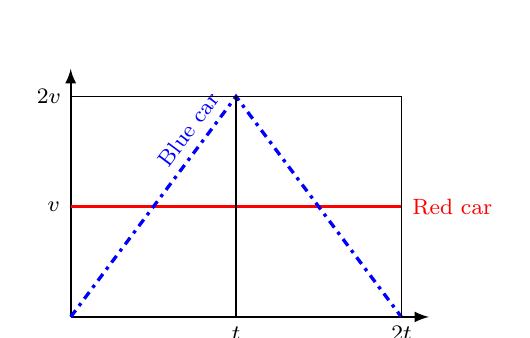
\begin{tikzpicture}[scale=.7]
        \draw[axes] (0,0)--(6.5,0);
        \draw[axes] (0,0)--(0,4.5);
        \draw[very thick,red] (0,2)--(6,2) node[pos=0,left,black]{$v$}
        node[right]{Red car};
        \draw[very thick,dash dot,blue] (0,0)--(3,4)
        node[pos=.8,above,sloped,dash dot,blue]{Blue car} --(6,0);
        \draw (0,4)--(6,4) node[pos=0,left]{$2v$};
        \draw (3,0)--(3,4) node[pos=0,below]{$t$};
        \draw (6,0)--(6,4) node[pos=0,below]{$2t$};
      \end{tikzpicture}
    \end{center}
    \begin{enumerate}[noitemsep]
    \item The blue car has travelled further, and both cars have the
      same instantaneous velocity
    \item Both cars have travelled the same distance, and the blue
      car has a greater instantaneous velocity
    \item The red car has travelled further, and both cars have the same
      instantaneous velocity
    \item Both cars have travelled the same distance, and both cars have the
      same instantaneous velocity
    \item The blue car has travelled further, and the blue car has a greater
      instantaneous velocity
    \end{enumerate}
    
  \item A car is travelling west and approaching a stop sign. As it is
    slowing to a stop, the directions associated with the object's velocity and
    acceleration, respectively, are
    \begin{enumerate}[noitemsep]
    \item West, East
    \item West, West
    \item East, East
    \item East, West
    \item There is not enough information to tell
    \end{enumerate}
    
  %\item The direction equivalent to [\ang{40} W of S] is
  %  \begin{enumerate}[noitemsep]
  %  \item [\ang{40} E of S]
  %  \item [\ang{40} W of N]
  %  \item [\ang{40} E of N]
  %  \item [\ang{50} S of W]
  %  \item [\ang{50} E of N]
  %  \end{enumerate}

  \item If a car travelling at \SI{60}{\kilo\metre\per\hour} [S] stops
    in a time of \SI{3.5}\second, its acceleration is:
    \begin{enumerate}[noitemsep]
    \item \SI{4.77}{\metre\per\second\squared} [S]
    \item \SI{4.77}{\metre\per\second\squared} [N]
    \item \SI{16.7}{\metre\per\second\squared} [S]
    \item \SI{16.7}{\metre\per\second\squared} [N]
    \item \SI{17.1}{\metre\per\second\squared} [S]
    \end{enumerate}

  \item Which of the following objects are in ``free fall''?
    \begin{enumerate}[noitemsep]
    \item A ball that was thrown horizontally
    \item A ball that was thrown at an angle above horizontal
    \item A ball that was thrown at an angle below horizontal
    \item A ball that was dropped
    \item All of the above
  \end{enumerate}
    
  \item An airplane is flying to a city due south from its current location. If
    there is a slight wind blowing to the south-east, the plane must head
    (point) to the:
    \begin{enumerate}[noitemsep]
    \item South
    \item West
    \item South-west
    \item South-east
    \item East
    \end{enumerate}

  \item A ball is thrown up in the air and then caught at the same height.
    The acceleration is \SI{9.81}{\metre\per\second\squared} [down]
    \begin{enumerate}[noitemsep]
    \item on the way up
    \item on the way down
    \item at the peak of its trajectory
    \item two of A, B, and C are correct
    \item all of A, B, and C are correct
  \end{enumerate}

  \item Two velocity vectors $v_1$ and $v_2$ each have the same magnitude.
    Graph 1 shows the velocity $v_1$ at $t=\SI0\second$, and then the same
    object has a velocity $v_2$ at $t=\SI2\second$, shown in Graph 2. Which of
    the following vectors best represents the average acceleration vector that
    causes the object's velocity to change from $v_1$ to $v_2$ ?
    \begin{center}
      \begin{tikzpicture}[scale=.6]
        \draw (-2,0)--(2,0);
        \draw (0,-2)--(0,2);
        \draw[vectors] (0,0)--(1.8,0) node[above]{$v_1$};
      \end{tikzpicture}
      \hspace{.2in}
      \begin{tikzpicture}[scale=.6]
        \draw (-2,0)--(2,0);
        \draw (0,-2)--(0,2);
        \draw[vectors] (0,0)--(0,1.8) node[right]{$v_2$};
      \end{tikzpicture}
    \end{center}
    A. \begin{tikzpicture}[scale=.6]
      \draw (-2,0)--(2,0);
      \draw (0,-2)--(0,2);
      \draw[vectors] (0,0)--(0,1.8);
    \end{tikzpicture}
    \hspace{.2in}
    B. \begin{tikzpicture}[scale=.6]
      \draw (-2,0)--(2,0);
      \draw (0,-2)--(0,2);
      \draw[vectors] (0,0)--(1.8,0);
    \end{tikzpicture}
    \hspace{.2in}
    C. \begin{tikzpicture}[scale=.6]
      \draw (-2,0)--(2,0);
      \draw (0,-2)--(0,2);
      \draw[vectors] (0,0)--(-1.8,0);
    \end{tikzpicture}
    \hspace{.2in}
    D. \begin{tikzpicture}[scale=.6]
      \draw (-2,0)--(2,0);
      \draw (0,-2)--(0,2);
      \draw[vectors,rotate=-45] (0,0)--(0,1.8);
    \end{tikzpicture}
    \hspace{.2in}
    E. \begin{tikzpicture}[scale=.6]
      \draw (-2,0)--(2,0);
      \draw (0,-2)--(0,2);
      \draw[vectors,rotate=45] (0,0)--(0,1.8);
    \end{tikzpicture}
  
  \item A passenger on a train moving horizontally at a constant speed
    relative to the ground drops a ball from his window. A stationary observer
    on the ground sees the ball falling with a speed $v_1$ at an angle to
    the vertical at an instant after it is dropped from the train window, but
    the ball appears to be falling vertically with a speed $v_2$ at the same
    instant as viewed by the train passenger. What is the speed (magnitude of
    velocity) of the train relative to the ground after the ball is dropped?
    Neglect air resistance.
    \begin{enumerate}[noitemsep]
    \item $v_1 + v_2$
    \item $v_1-v_2$
    \item $v_1^2 + v_2^2$
    \item $v_1^2-v_2^2$
    \item $\sqrt{v_1^2-v_2^2}$
    \end{enumerate}
    
  \item A ball is dropped from rest from the top of a cliff \SI{80}{\metre}
    high. At the same time, a rock is thrown horizontally from the top of the
    same cliff. The rock and ball hit the level ground below a distance of
    \SI{40}{\metre} apart. The horizontal velocity of the rock that was thrown
    was most nearly
    \begin{center}
      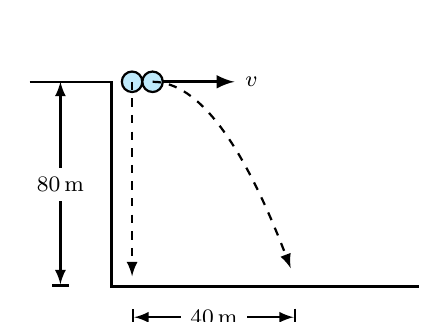
\begin{tikzpicture}[scale=1.3]
        \draw[thick] (-.8,0)--(0,0)--(0,-2)--(3,-2);
        \draw[thick,<->|](-.5,0)--(-.5,-2) node[midway,fill=white]{\SI{80}\metre};
        \draw[mass] (.2,0) circle (.1);
        \draw[mass] (.4,0) circle (.1);
        \draw[vectors] (.5,0)--(1.2,0) node[right]{$v$};
        \draw[axes,dashed] (.2,0)--(.2,-1.9);
        \draw[axes,dashed] plot[smooth,domain=.4:1.75] (\x, {-(\x-.4)^2});
        \draw[thick,|<->|] (.2,-2.3)--(1.8,-2.3)
        node[midway,fill=white]{\SI{40}\metre};
      \end{tikzpicture}
    \end{center}
    \begin{enumerate}[noitemsep]
    \item\SI5{\metre\per\second}
    \item\SI{10}{\metre\per\second}
    \item\SI{20}{\metre\per\second}
    \item\SI{40}{\metre\per\second}
    \item\SI{80}{\metre\per\second}
    \end{enumerate}
  
  \item A golf ball is hit from level ground and has a horizontal range of
    100 m. The ball leaves the golf club at an angle of \ang{60} to the level
    ground. At what other angle(s) can the ball be struck at the same initial
    velocity and still have a range of 100 m?
    \begin{center}
      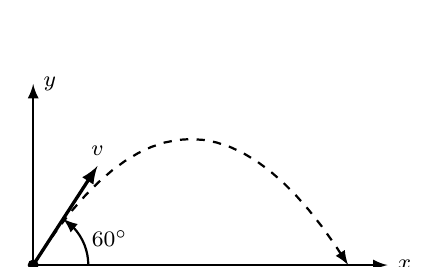
\begin{tikzpicture}
        \draw[axes] (0,0)--(4.5,0) node[right]{$x$};
        \draw[axes] (0,0)--(0,2.3) node[right]{$y$};
        \fill circle (.07);
        \draw[vectors,rotate=57] (0,0)--(1.5,0) node[above]{$v$};
        \draw[thick,dashed,->,domain=0:4] plot(\x,{-.4*((\x-2)*(\x-2))+1.6});
        \draw[axes] (.7,0) arc (0:57:.7) node[midway,right]{\ang{60}};
      \end{tikzpicture}
    \end{center}
    \begin{enumerate}[noitemsep]
    \item\ang{30}
    \item\ang{20} and \ang{80}
    \item\ang{10} and \ang{120}
    \item\ang{45} and \ang{135}
    \item There is no other angle other than \ang{60} in which the ball will
      have a range of 100 m.
  \end{enumerate}
  
  \item The motion of an object is represented by the acceleration vs.\ time
    graph below. If the object is initially at rest, which of the
    following statements is true about its motion?
    \begin{center}
      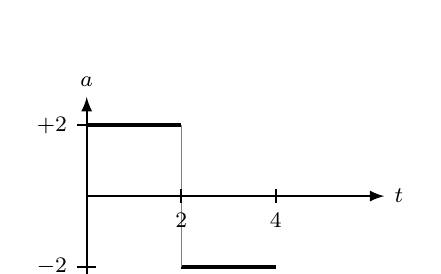
\begin{tikzpicture}[yscale=.45,xscale=.6]
        \draw[axes] (0,0)--(6.3,0) node[right]{$t$};
        \draw[axes] (0,-2.5)--(0,2.8) node[above]{$a$};
        \draw[ultra thick] (0,2)--(2,2);
        \draw[ultra thick] (2,-2)--(4,-2);
        \draw[gray] (2,2)--(2,-2);
        \draw[thick] (2,.2)--(2,-.2) node[below]{2};
        \draw[thick] (4,.2)--(4,-.2) node[below]{4};
        \draw[thick] (.2,2)--(-.2,2) node[left]{$+2$};
        \draw[thick] (.2,-2)--(-.2,-2) node[left]{$-2$};
      \end{tikzpicture}
    \end{center}
    \begin{enumerate}[noitemsep]
    \item The object returns to its original position.
    \item The velocity of the object is zero at a time of \SI2\second.
    \item The velocity of the object is zero at a time of \SI4\second.
    \item The displacement of the object is zero at a time of \SI4\second.
    \item The acceleration of the object is zero at a time of \SI2\second.
    \end{enumerate}
    
  \item Can an object ever be accelerating and experiencing an
    instantaneous velocity of \SI0{\metre\per\second}? Explain. 
    
  \item Large insects such as locusts can jump as far as \SI{75}{cm}
    horizontally on a level surface. An entomologist analyzed a photograph and
    found that the insect's launch angle was \ang{55}. What was the insect's
    initial velocity?
  
  \item Because of an oncoming storm, a boat must cross a river in the
    shortest amount of time possible regardless of where it lands on the
    opposite shore. Given that the river has a current, in what direction
    should the boat point? Explain.
    \vspace{\stretch1}
  
  \item While hiking in the wilderness, you come to the top of a cliff that
    is \SI{60}{\metre} high. You throw a stone from the cliff, giving it an
    initial velocity of \SI{21}{\metre\per\second} at \ang{35} above the
    horizontal. How far from the base of the cliff does the stone land?
    \vspace{\stretch2}
  
  \item You want to shoot a stone with a sling shot and hit a target on the
    ground \SI{14.6}{\metre} away. If you give the stone an initial speed of
    \SI{12.5}{\metre\per\second}, neglecting friction and air resistance, what
    is/are the launch angle(s) in order for the stone to hit the target? What
    would be the maximum height(s) by the stone? What would be its time of
    flight? Assume motion is symmetric.
  
  \item A sharpshooter shoots a bullet horizontally over level ground with
    a velocity of \SI{1.22e3}{\metre\per\second}. At the instant that the bullet
    leaves the barrel, its empty shell casing falls vertically and strikes the
    ground with a vertical velocity of \SI{5.50}{\metre\per\second}.
    \begin{enumerate}
      \item Neglecting air friction, how far does the bullet travel?
      \item What is the vertical component of the bullet's velocity at the
      instant before it hits the ground?
    \end{enumerate}

  \item A projectile is launched from point $O$ at an angle of \ang{22} with
    an initial velocity of $v_0=\SI{15}{\metre\per\second}$ up an incline plane
    that makes an angle of \ang{10} with the horizontal. The projectile lands on
    the incline plane at point $M$.
    \begin{center}
      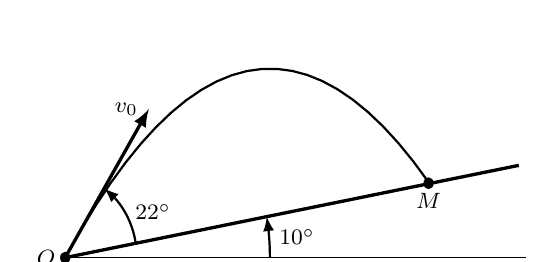
\begin{tikzpicture}[xscale=1.3,yscale=1.5]
        \draw (0,0)--(4.5,0);
        \fill circle (.05) node[left]{$O$};
        \draw[vectors,rotate=57] (0,0)--(1.5,0) node[left]{$v_0$};
        \draw[thick,domain=0:3.55] plot(\x,{-.4*((\x-2)*(\x-2))+1.6});
        \draw[axes,rotate=10] (.7,0) arc(0:47:.7) node[midway,right]{\ang{22}};
        \draw[very thick,rotate=10] (0,0)--(4.5,0);
        \draw[axes] (2,0) arc (0:10:2) node[midway,right]{\ang{10}};
        \fill (3.55,.63) circle (.05) node[below]{$M$};
      \end{tikzpicture}
    \end{center}
    \begin{enumerate}
      \item Find the time it takes for the projectile to hit the incline plane.
      \item Find the distance $OM$.
    \end{enumerate}
    
  \item A baseball is thrown by an outfielder ($O$) towards the catcher
    ($C$) with an initial speed of \SI{20}{\metre\per\second} at an angle of
    \ang{45} with the horizontal. At the moment that the ball is thrown, $C$ is
    \SI{50}{\metre} from $O$. At what speed and in what direction must $C$ run
    to catch the ball at the same height at which it was released? Assume that
    $C$ catches the ball at the same moment that it arrives. Please answer in
    two significant figures.

  \item A car is travelling north on a city street at
    \SI{12.5}{\metre\per\second}. Just as the car crosses a perpendicularly
    intersecting crossroad, the passenger throws out a can horizontally, towards
    the east. The initial speed of the can relative to the car is
    \SI{10.0}{\metre\per\second}. It is released at a height of 1.75 m above the
    road.
    \begin{enumerate}
      \item What is the initial velocity of the can relative to the road?
      \item Where does the can land relative to the centre of the intersection?
    \end{enumerate}
  
%  %\item An object is thrown upward on a slope and reached a height of
%  %$h=\SI{15}{\metre}$ as shown, the object lands near the base of slope at a
%  %distance of $l=\SI{75}{\metre}$ away. The slope angle $\alpha$ is \ang{35}.
%  %\begin{center}
%  %  \pic{.35}{../graphics/FF55a}
%  %\end{center}
%  %Determine
%  %\begin{parts}
%  %\item the magnitude $v$, and
%  %\item the direction of the initial velocity $\theta$
%  %\end{parts}
  \end{enumerate}
\end{multicols}



\part{Dynamics}

%\usetikzlibrary{decorations.pathmorphing,patterns}

\chapter{Dynamics}
\label{chapter:dynamics}

%\section[Intro]{Introduction}

Now that we can mathematically describe the motion of any object, we have to
be able describe \emph{what} causes motion, or more precisely,
\emph{what causes motion to change.}




\section{Laws of Motions}
The definitions given here are based on the original text by Newton in
\emph{Principia}, but with some wording replaced with modern physics
language\footnote{For example, Newton used the term \emph{the alteration of
motion} to describe the acceleration of the object.}

The first law of motion describes what happens when there are no forces act on
an object:
\begin{definition}
  \textbf{First law:} Every object remains at rest or in uniform motion, until
  there is a net external force acting on the object.
\end{definition}
In other words, when the vector sum of all the forces acting on an object is
zero, the object's velocity does not change. In other words, the three equations
below are equivalent:
\begin{equation*}
  \bm F_\text{net}=\sum\bm F=\bm 0
  \quad\longleftrightarrow\quad
  \bm v=\text{constant}
  \quad\longleftrightarrow\quad
  \bm a=\bm 0
\end{equation*}
%  \end{center}
%  \begin{itemize}
%  \item As long as an object moves in uniform motion, it must be that
%    $\bm F_\text{net}=\bm 0$
%  \item Examples:
%    \begin{itemize}
%    \item A spacecraft in ``deep space'' has no forces acting on it
%    \item A hockey puck sliding on very smooth ice has gravity and normal
%      force, but the net force is zero
%    \item A car travelling on a highway at \SI{100}{\kilo\metre\per\hour} has
%      many forces acting on it, but the net force is zero
%    \end{itemize}
%  \item In ``a state of equilibrium''
%  \end{itemize}

What is not stated explicitly by Newton is that the first law of motion is only
valid when the mass of the object is constant. In other words, the first law of
motion, as stated above, will \emph{not} work for:
\begin{itemize}[itemsep=3pt]
\item A rocket expelling spent fuel as it is launched towards space
\item A train car collecting grain though its open top
\end{itemize}
Later in Chapter~\ref{chapter:momentum}, we will modify the first law of motion
to include objects with changing mass.


The secon law of motion addresses what happens when the forces acting on an
object is not balance, i.e.\ when the net force is not zero.

\begin{definition}
  \textbf{Second law:} The acceleration of an object is proportional to the
  sum of all forces (net force) acting on it; and is along the same
  direction as the net force.
\end{definition}
The second law states that the acceleration of an object is the directresult of
the imbalance of forces, and that the relationship is \emph{linear} (i.e.\ when
the net force is double, the acceleration also doubles).

The first two laws of motion can be summarized by perhaps one of the most
important and recognizable equations in physics:
\begin{equation}
  \boxed{\bm F_\text{net}=m\bm a}
\end{equation}
The \emph{proportionality} between the net force and the acceleration of the
object is its mass. In fact, mass is defined as the ratio between the magnitude
of the net force acting on an object and the magnitude of the resultant
acceleration:
\begin{equation}
  m=\frac{|\bm F_\text{net}|}{|\bm a|}
\end{equation}
As such, mass is an intrinsic property of an object, and the same net force on
the object will \emph{always} result in the same acceleration, regardless of
what the net force is composed of, and whether the object is on Earth, on the
Moon, or in deep space.

Both the first and second laws of moton, as stated by Newton, require that the
mass of the object be constant. 




The third law of motion deals with the interaction between objects when forces
are created, and how objects apply forces on each other:
\begin{definition}
  \textbf{Third Law:} To every action there is always opposed and equal
  reaction; the mutual actions of two bodies upon each other are always
  equal, and directed to contrary parts.
\end{definition}
Mathematically, we can write that the force object $A$  exerts on bbject $B$
($\bm F_{AB}$, the action force) is equal in magnitude but opposite in
direction to the force that object $B$ exerts on object $A$ ($\bm F_{BA}$, the
reaction force).
\begin{equation}
  \boxed{\bm F_\text{AB} = -\bm F_\text{BA}}
  \label{eq:third-law}
\end{equation}
The negative sign in Eq.~\ref{eq:third-law} indicates that the forces are in
opposite direction. It must be noted that
\textbf{the action and reaction forces must act on \emph{different} objects}.

The implication of the laws of motion is that forces are always created in
pairs: it is impossible for one object to exert a force on another without also
simultaneously being acted on by the other object. In
Chapter~\ref{chapter:energy}, we will show that the third law of motion is
crucial in formulating, and understanding, the law of conservation of energy.
In Chapter~\ref{chapter:momentum}, we will show that the third law of motion
is, in fact, an application of the first law of motion.

%\begin{example}
%  Old-style television picture tubes and computer monitors use cathode ray
%  tubes, where light is produced when fast-moving electrons collide with
%  phosphor molecules on the surface of the screen. The electrons (mass
%  $m=\text{\SI{9.1e-31}{\kilo\gram}}$) are accelerated from rest in the
%  electron ``gun'' at the back of the vacuum tube. Find the velocity of an
%  electron when it exits the gun after experiencing an electric force of
%  \SI{5.8e-15}{\newton} over a distance of \SI{3.5}{\milli\metre}.
%\end{example}

\section{Common Forces}
%  \textbf{Force} is the interaction between the objects
%  \begin{itemize}
%  \item When there is interaction, then forces are created
%  \item A ``push'' or a ``pull''
%  \end{itemize}
%
%  \vspace{.2in}There are two types of forces:
%  \begin{itemize}
%  \item\textbf{Contact forces} act between two objects that are in contact
%    with one another
%  \item\textbf{Non-contact forces} act between two objects without them
%    touching each other.
%    \begin{itemize}
%    \item Also called ``action-at-a-distance'' force
%    \end{itemize}
%  \end{itemize}
%
%
%
%
%\section{Forces}
%  Newton considered all forces acting at a single point of an object called the
%  centre of mass (``CM'')
%  \begin{itemize}
%  \item The centre of mass is also called the centre of gravity (``CG'') if the
%    object is inside a uniform gravitational field\footnote{Gravitational field
%    is a topic that will be discussed in Class 7}
%  \item If the density of an object is constant, then the CM is also the
%    geometric centre (centroid) of the object
%  \end{itemize}
%%  \vspace{.2in}If the net force on an object is zero ($\sum\bm F=\bm{0}$)
%%  then the object is in a \emph{state of equilibrium}
%%  \begin{itemize}
%%  \item Dynamic equilibrium: the object is moving relative to us
%%  \item Static equilibrium: the object is not moving relative to us
%%  \end{itemize}




\begin{itemize}[noitemsep]
\item Gravitational force ($\bm F_g$)
\item Normal force ($\bm F_n$)
\item Static and kinetic friction ($\bm F_s$ and  $\bm F_k$)
\item Spring force ($\bm F_e$)
\item Tension ($\bm F_T$)
\item Fluid Resistance, or Drag ($\bm F_d$)
\item Applied force ($\bm F_a$)
\item Electrostatic force ($\bm F_q$, discussed in Unit 3)
\item Magnetic force ($\bm F_m$, discussed in Unit 3)
\end{itemize}




\subsection{Gravity}
\textbf{Gravity} is the mutual force of attraction between all massive objects.
The gravitational force that objects apply to each other can be expressed as:
\begin{equation}
  \boxed{\bm F_g=m\bm g}
\end{equation}
The gravitational force acts in the same direction as $\bm g$, the acceleration
due to gravity at the object's position. At or near the surface of Earth,
$\bm g=\text{\SI{9.81}{\metre\per\second\squared}}$ [down]. In fact, the
direction of $\bm g$ is how we \emph{define} the concept of ``down''. $\bm g$
is also known as the ``gravitational field''; will be discussed in depth in
Chapter~\ref{chapter:gravity}. If this is the only force that acts on an object,
its resulting motion is called \textbf{free fall}.

To be clear, by the third law of motion, any object that is subjected to the
gravitational pulled by Earth will also exert an equal and opposite force on
Earth. However, since Earth is much more massive, this force will have no
effect to Earth's motion.

\subsection{Normal Force}
\textbf{Normal force} $F_n$ is a force a surface exerts on another object
that it is in contact with. It is always \emph{perpendicular} to the contact
surface.\footnote{This is where the term \emph{normal} came from.}

\begin{figure}[ht]
  \centering
  \begin{tikzpicture}
    \draw[thick] (-1,0)--(2.5,0);
    \draw[mass] rectangle (1.5,1);
    \fill (.75,.5) circle (2pt);
    \draw[vectors] (.75,.5)--+(0,-1) node[below]{$F_g$};
    \draw[vectors] (.75,.5)--+(0,1) node[above]{$F_n$};
  \end{tikzpicture}
  \hspace{.5in}
  \begin{tikzpicture}
    \begin{scope}[rotate=30]
      \draw[thick] (-1,0)--(2.5,0);
      \draw[mass] rectangle (1.5,1);
      \fill (.75,.5) circle (2pt);
      \begin{scope}[vectors]
        \draw[rotate around={-30:(.75,.5)}] (.75,.5)--+(0,-1)
        node[below]{$F_g$};
        \draw (.75,.5)--+(0,1) node[above]{$F_n$};
      \end{scope}
    \end{scope}
  \end{tikzpicture}
\end{figure}
Regardless of whether the surface is horizontal or slanted, $F_n$ is always be
perpendicular to the surface. However, the \emph{magnitude} of the normal force
will change.




%%\section{Normal Force on an Incline}
%%  When an object sits on a stationary incline, normal force decreases.
%%  
%%    \centering
%%    \begin{tikzpicture}[scale=.9]
%%      \draw[thick] (-1,0)--(3,0);
%%      \draw[thick,->] (0,0) arc (0:37:1) node[midway,right] {$\theta$};
%%      \begin{scope}[rotate around={37:(-1,0)}]
%%        \draw[->](3.5,.5)--(4,.5)  node[right]{$x$};
%%        \draw[->](3.5,.5)--(3.5,1) node[above]{$y$};
%%        \draw[thick] (-1,0)--(4,0);
%%        \draw[fill=pink,thick] rectangle (3,2);
%%        \fill(1.5,1) circle (.07) node[right]{CM};
%%        \begin{scope}[->,thick,red]
%%          \draw[dotted] (1.5,1)--(1.5,-.5) node[right]{$F_g\cos\theta$};
%%          \draw[dotted] (1.5,1)--(.45,1) node[left]{$F_g\sin\theta$};
%%        \end{scope}
%%        \draw[->,very thick,red] (1.5,1)--(.45,-.5)
%%        node[below]{$F_g$}
%%        node[pos=.3,below right]{$\theta$};
%%        \draw[->,very thick] (1.5,1)--(1.5,2.5) node[above]{$F_n$};
%%      \end{scope}
%%    \end{tikzpicture}
%%    
%%    \begin{itemize}
%%    \item $F_n=F_g\cos\theta$
%%    \item $F_g$ has a component along the ramp $F_g\sin\theta$ that
%%      wants to slide the block down.
%%    \item There may also be a friction force $F_f$ that opposes the motion
%%    \item If the incline is also accelerating, then we have to treat this
%%      problem as a connected-body problem (discussed later in this topic)
%%    \end{itemize}

\subsection{Friction}
\textbf{Friction} is force that opposes the sliding of two surface across one
another
\begin{itemize}
\item Always act in the direction opposite to motion or attempted motion
\item Two types: \emph{static friction} and \emph{kinetic friction}
\end{itemize}  
%  \begin{center}
%   \pic{.6}{graphics/friction}
%  \end{center}


\textbf{Static friction} is the resistive force between two surfaces when
there is no relative motion between them. It increases with increasing
applied force $F_a$. It is at maximum when the object is just about to move.
\begin{equation}
  \boxed{
    F_s \leq \mu_sF_n
  }
  \label{eq:static-friction}
\end{equation}
\begin{center}
  \begin{tabular}{l|c|c}
    \rowcolor{pink}
    \textbf{Quantity} & \textbf{Symbol} & \textbf{SI Unit} \\ \hline
    Magnitude of static friction   & $F_s$ & \si\newton \\
    Coefficient of static friction & $\mu_s$ & (no unit)\\
    Magnitude of normal force      & $F_n$ & \si\newton
  \end{tabular}
\end{center}
Equation~\ref{eq:static-friction} only deals with the \emph{magnitude} of the
force. A proper free-body diagram is required to express the direction of
$\bm F_s$
%  \begin{tikzpicture}[overlay]
%    \uncover<2>{
%      \node[text width=85,draw=violet,fill=violet!5,text=violet] (act) at
%      (-3.2,4) {Actual static friction};
%      \draw[axes,violet] (act)--+(3,0);
%      
%      \node[text width=100,draw=orange,fill=orange!5,text=orange] (max) at
%      (5.05,4) {Maximum static friction};
%      \draw[axes,orange] (max)--+(-3,0);
%    }
%  \end{tikzpicture}

\textbf{Kinetic friction} is the resistive force between two surfaces that
are moving relative to each other. It is (nearly) constant along the path of
movement as long as the normal force stays constant:
\begin{equation}  
  \boxed{F_k = \mu_kF_n}
\end{equation}
\begin{center}
  \begin{tabular}{l|c|c}
    \rowcolor{pink}
    \textbf{Quantity} & \textbf{Symbol} & \textbf{SI Unit} \\ \hline
    Magnitude of kinetic friction   & $F_k$   & \si{\newton}\\
    Coefficient of kinetic friction & $\mu_k$ & (no unit)\\
    Magnitude of normal force       & $F_n$   & \si{\newton}
  \end{tabular}
\end{center}    
$\mu_k$ is always lower than $\mu_s$, otherwise nothing will ever move:
\begin{equation}  
  \mu_k\leq\mu_s
\end{equation}

%  \begin{tikzpicture}[overlay]
%    \uncover<2>{
%      \node[text width=86,draw=magenta,fill=magenta!5,text=magenta] (act) at
%      (3.5,5) {Unlike static friction, this is an equality};
%      \draw[axes,magenta] (act) to[out=50,in=90] +(3.5,.25);
%    }
%  \end{tikzpicture}




\subsection{Tension in a Cable}
\textbf{Tension} is the force exerted on and by a cable, rope, or string.
\begin{itemize}
\item You can't push on a rope
\item Assume the cable/rope/string to be mass less
\item Force can change direction when used with pulleys
\end{itemize}
How do engineers determine the amount of tension needed for a specific object
(bridges, floors or light fixtures)?




\subsection{Spring Force}
The spring force $\bm F_e$ is the force that a compressed/stretched spring
exerts on the object connected to it. An \emph{ideal} spring obeys
\textbf{Hooke's law}:
\begin{equation}
  \boxed{
    \bm F_e=-k\bm x
  }
\end{equation}
$\bm F_e$ is in the opposite direction to the spring's displacement $\bm x$,
and is proportional to the amount of compression/stretching.

\begin{center}
  \begin{tikzpicture}[scale=.8]
    \draw[mass] (5,.5) rectangle (6,1.5);
    \draw[thick,
      decoration={aspect=.6,segment length=5mm, amplitude=2.5mm, coil},
      decorate] (0,1)--(5,1);
    \fill[pattern=north east lines](-.2,0) rectangle (0,2);
    \draw[thick] (0,0)--(0,2);
    \fill[red] (5.5,1) circle (.06);
    \draw[vectors,red] (5.5,1)--(4,1) node[above]{$\bm F_e$};
    \draw[dashed] (3,0)--(3,2) node[above]{Equilibrium position};
    \draw[vectors] (3,.3)--(5,.3) node[midway,below]{$x$};
  \end{tikzpicture}
  \hspace{.2in}
  \begin{tikzpicture}[scale=.8]
    \draw[thick,gray!40,fill=gray!20] (5,.5) rectangle (6,1.5);
    \draw[thick,gray!20,
      decoration={aspect=.6,segment length=5mm, amplitude=2.5mm, coil},
      decorate] (0,1)--(5,1);
    \fill[pattern=north east lines] (-.2,0) rectangle(0,2);
    \draw[thick] (0,0)--(0,2);
    \fill[gray!30] (5.5,1) circle (.06);
    \draw[vectors,gray!30] (5.5,1)--(4,1) node[above]{$\bm F_e$};
    \draw[dashed] (3,0)--(3,2);
    \draw[vectors,gray!30] (3,.3)--(5,.3) node[midway,below]{$x$};
    \draw[mass] (1.5,.5) rectangle (2.5,1.5);
    \draw[thick,
      decoration={aspect=.3,segment length=1.5mm, amplitude=2.5mm, coil},
      decorate] (0,1)--(1.5,1);
    \draw[vectors] (3,.3)--(1.5,.3) node[midway,below]{$x$};
    \fill[red] (2,1) circle (.06);
    \draw[vectors,red] (2,1)--(3,1) node[above]{$\bm F_e$};
  \end{tikzpicture}
\end{center}
The constant $k$ (called the \textbf{spring constant}, \textbf{force
  constant}, \textbf{Hooke's constant} or \textbf{spring rate}) is the
stiffness of the spring. It has a unit of \si{\newton\per\metre}.



\subsection{Fluid Resistance (Drag)}

When an object (e.g.\ an aircraft, a bicycle or a car) moves through air, or
when a submarine moves under water, they all experience a
fluid\footnote{A gas or a liquid} resistance force called the
\textbf{drag} $\bm F_d$.
\begin{figure}[ht]
  \centering
  \begin{subfigure}{.338\textwidth}
    \pic1{dynamics/boeing787}
    \caption{A commercial aircraft flying through air}
  \end{subfigure}
  \begin{subfigure}{.35\textwidth}
    \pic1{dynamics/ganna}
    \caption{A cyclist riding at high speed during a bike race}
  \end{subfigure}
  \begin{subfigure}{.263\textwidth}
    \pic1{dynamics/submarine}
    \caption{A submarine moving through water}
  \end{subfigure}
\end{figure}
The drag force is experienced by any object moving through a fluid. The
direction of drag is in the opposite direction to the velocity vector.

There are multiple sources of drag:
\begin{itemize}
\item\textbf{form drag} is due to the shape of the object
\item\textbf{skin friction} is due to the friction of the fluid against
  the surface of the object moving through it
\item\textbf{interference drag} is due to when airflow around one part of
  an object occupying the same space as the airflow around another part
  (e.g.\ fuselage and wing of an airplane)
\end{itemize}

Unlike kinetic friction (which is constant), drag depend on the speed of the
moving object, as well as its shape:
\begin{equation}
  \boxed{
    F_d=\frac12\rho v_\infty^2C_DA_\text{ref}
  }
\end{equation}
\begin{center}
  \begin{tabular}{l|c|c}
    \rowcolor{pink}
    \textbf{Quantity} & \textbf{Symbol} & \textbf{SI Unit} \\ \hline
    Magnitude of drag       & $F_d$     & \si\newton \\
    Density of the fluid    & $\rho$    & \si{\kilo\gram\per\metre\cubed}\\
    Free-stream velocity    & $v_\infty$ & \si{\metre\per\second} \\
    Reference area          & $A_\text{ref}$ & \si{\metre\squared} \\
    Drag coefficient        & $C_D$     & (no unit)
  \end{tabular}
\end{center}
$C_D$ depends on the shape and surface smoothness of the object; for bluff
bodies $A_\text{ref}$ is the frontal area; for streamlined objects
$A_\text{ref}$ is the planform (top-view) area




\section{Free Body Diagrams}
A free-body diagram is used to visualize the forces acting on an object. It is
very useful tool that should be used all the time.
\emph{We generally draw the forces from an inertial frame of reference.}

\begin{enumerate}
\item Draw a ``big dot'' to represent the centre of mass of the object.
%  \vspace{.1in}
%  
%    \centering
%    \begin{tikzpicture}[scale=.8]
%      \draw[lightgray,thick] (-1,0)--(4,0);
%      \draw[lightgray,fill=cyan!10,thick] rectangle (3,2);
%      \fill (1.5,1) circle (.1) node[above]{CM};
%    \end{tikzpicture}
%    
%    \centering
%    \begin{tikzpicture}[scale=.8]
%      \begin{scope}[rotate=30]
%        \draw[lightgray,thick] (0,0)--(5,0);
%        \draw[lightgray,fill=cyan!10,thick] (1,0) rectangle (4,2);
%        \fill (2.5,1) circle (.1) node[above]{CM};
%      \end{scope}
%      \draw[lightgray,thick] (0,0)--(4.5,0);
%    \end{tikzpicture}
%    
%    \centering
%    \begin{tikzpicture}[scale=.8]
%      \draw[lightgray,fill=cyan!10,thick] circle (.5);
%      \fill circle (.1) node[above]{CM};
%    \end{tikzpicture}
%  
%
%
%
%
%\section{Free Body Diagrams}
\item Define a coordinate system ($x$ and $y$ axes)
  \begin{itemize}
  \item Axes are defined to simplify the problem (not to make it more
    complicated!)
  \item Define coordinate system such that motion is along one axis (usually
    $x$) only
  \end{itemize}

%  \vspace{.1in}
%  
%    \centering
%    \begin{tikzpicture}[scale=.8]
%      \draw[lightgray,thick] (-1,0)--(4,0);
%      \draw[lightgray,fill=cyan!10,thick] rectangle (3,2);
%      \fill (1.5,1) circle (.1);
%      \draw[axes] (3.5,.5)--(4.5,.5) node[right]{$x$};
%      \draw[axes] (3.5,.5)--(3.5,1.5) node[above]{$y$};
%    \end{tikzpicture}
%    
%    \centering
%    \begin{tikzpicture}[scale=.8]
%      \begin{scope}[rotate=30]
%        \draw[lightgray,thick] (0,0)--(5,0);
%        \draw[lightgray,fill=cyan!10,thick] (1,0) rectangle (4,2);
%        \fill (2.5,1) circle (.1);
%        \draw[axes] (4.5,.5)--(5.5,.5)  node[right]{$x$};
%        \draw[axes] (4.5,.5)--(4.5,1.5) node[above]{$y$};
%      \end{scope}
%      \draw[lightgray,thick] (0,0)--(4.5,0);
%    \end{tikzpicture}
%    
%    \centering
%    \begin{tikzpicture}[scale=.8]
%      \draw[lightgray,fill=cyan!10,thick] circle (.5);
%      \fill circle (.1);
%      \draw[axes] (1,0)--(2,0) node[right]{$x$};
%      \draw[axes] (1,0)--(1,1) node[above]{$y$};
%    \end{tikzpicture}
%
%
%
%
%
%\section{Free Body Diagrams}
\item Identify and label all forces acting on the object
  \begin{itemize}
  \item If it has mass, weight $\bm F_g$ acts downward
  \item If it is on a surface, there is also a normal force $\bm F_n$
  \item If there is friction, first think about which direction the object will
    move without it, then draw $\bm F_s$ or $\bm F_k$ in the opposite
    direction
  \item If it is being pushed/pulled, there may be an applied force
    $\bm F_a$ or tension force $\bm F_T$
  \end{itemize}

%  
%    \centering
%    \begin{tikzpicture}[scale=.8]
%      \draw[lightgray,thick] (-1,0)--(4,0);
%      \draw[lightgray,fill=cyan!10,thick] rectangle (3,2);
%      \fill (1.5,1) circle (.1);
%      \draw[axes] (3.5,.5)--(4.5,.5) node[right]{$x$};
%      \draw[axes] (3.5,.5)--(3.5,1.5) node[above]{$y$};
%      \draw[vectors] (1.5,1)--(1.5,-.5) node[below]{$\bm F_g$};
%      \draw[vectors] (1.5,1)--(1.5,2.5) node[above]{$\bm F_n$};
%      \draw[vectors] (1.5,1)--(3.1,1) node[below]{$\bm F_a$};
%      \draw[vectors] (1.5,1)--(.75,1) node[left]{$\bm F_f$};
%    \end{tikzpicture}
%    
%    \centering
%    \begin{tikzpicture}[scale=.8]
%      \draw[lightgray,thick] (0,0)--(4.5,0);
%      \begin{scope}[rotate=30]
%        \draw[lightgray,thick] (0,0)--(5,0);
%        \draw[lightgray,fill=cyan!10,thick] (1,0) rectangle (4,2);
%        \fill (2.5,1) circle (.1);
%        \draw[axes] (4.5,.5)--+(1,0) node[right]{$x$};
%        \draw[axes] (4.5,.5)--+(0,1) node[above]{$y$};
%        \draw[vectors,rotate around={-30:(2.5,1)}] (2.5,1)--(2.5,-.5)
%        node[below]{$\bm F_g$};
%        \draw[vectors] (2.5,1)--(2.5,2.4) node[above]{$\bm F_n$};
%        \draw[vectors] (2.5,1)--(4.1,1) node[below]{$\bm F_a$};
%        \draw[vectors] (2.5,1)--(1.75,1) node[left]{$\bm F_f$};
%      \end{scope}
%    \end{tikzpicture}
%    
%    \centering
%    \begin{tikzpicture}[scale=.8]
%      \draw[lightgray,fill=cyan!10,thick] circle (.5);
%      \fill circle (.1);
%      \draw[axes] (1,0)--(2,0) node[right]{$x$};
%      \draw[axes] (1,0)--(1,1) node[above]{$y$};
%      \draw[vectors] (0,0)--(0,-1.5) node[below]{$\bm F_g$};
%    \end{tikzpicture}
\end{enumerate}  


\section{Examples of Free Body Diagrams}



\section{Solving Force Problem}
Once the free-body diagram has been drawn,
\begin{itemize}
\item Break down the forces into the $x$ and $y$ components
\item Sum forces in the direction that doesn't have a net force (usually
  $y$ axis)
\item Sum forces in the other axis, and find out what the acceleration is
\item Use kinematic equations to solve the motion of the object along that axis
\end{itemize}




\begin{example}
  To move a \SI{45}{\kilo\gram} wooden crate across a wooden floor
  ($\mu=0.20$), you tie a rope onto the crate and pull on the rope. While you
  are pulling the rope with a force of \SI{115}\newton, it makes an angle of
  \ang{15} with the horizontal. How much time elapses between the time at which
  the crate just starts to move and the time at which you are pulling it with a
  velocity of \SI{1.4}{\metre\per\second}?
%  \begin{center}
%    \pic{.4}{graphics/pull-box}
%  \end{center}
\end{example}

\begin{example}
  You are holding an \SI{85}{\kilo\gram} trunk at the top of a ramp that slopes
  from a moving van to the ground, making an angle of \ang{35} with the ground.
  You lose your grip and the trunk begins to slide.
  \begin{enumerate}
  \item If the coefficient of friction between the trunk and the ramp is 0.42,
    what is the acceleration of the trunk?
  \item If the trunk slides \SI{1.3}{\metre} before reaching the bottom of the
    ramp, for what time interval did it slide?
  \end{enumerate}
\end{example}

\begin{example}
  A \SI{55}{\kilo\gram} person is standing on a scale in an elevator. If the
  scale is calibrated in \emph{newtons}, what is the reading on the scale when
  the elevator is not moving? If the elevator begins to accelerate upward at
  \SI{.75}{\metre\per\second\squared}, what will be the reading on the scale?
\end{example}



\begin{example}
  An elevator filled with people has a total mass of \SI{2245}{\kilo\gram}. As
  the elevator begins to rise, the acceleration is
  \SI{.55}{\metre\per\second\squared}. What is the tension in the cable that is
  lifting the elevator?   
\end{example}



\section{Multi-Body Problems}
\begin{figure}[ht]
  \centering
  \pic1{dynamics/graphics/go-train}
  \caption{A train in motion can be treated as a single object, or a number of
    objects connected together.}
\end{figure}
%\begin{center}
%  \pic{.7}{graphics/worldslongestroadtrainwithpowertrailer8}
%\end{center}
%  \begin{itemize}
%  \item Usually the objects are connected by a cable or a solid linkage with
%    negligible mass
%  \item All objects have the same acceleration
%  \item Require multiple free-body diagrams
%  \end{itemize}
%
%
%
%
%\section{Solving Connected-Bodies Problems}
%  To solve a connected-bodies problem, you can follow these procedures:
%  \begin{enumerate}
%  \item Draw a free-body diagram (FBD) on each of the objects
%  \item Sum all the forces on all the objects along the direction of motion
%    \begin{itemize}
%    \item Direction of motion is usually very obvious
%    \item Action/reaction pairs of forces cancel, because they are
%      \emph{internal} forces %and not \emph{external} forces
%    \end{itemize}
%  \item Compute the acceleration of the entire system using the second law of
%    motion
%    \begin{itemize}
%    \item Remember that every object has the same acceleration!
%    \end{itemize}
%  \item Go back to the FBD of each of the objects and compute any unknown
%    forces
%  \end{enumerate}
%
%
%
%
\subsection{Objects Connected by Cables}
\begin{example}
  Three masses ($m_1$, $m_2$ and $m_3$) are connected by massless cables (we
  assume that he cables are very light compared to the masses, and so we can
  ignore them without making our answers inaccurate), and pulled to the right
  by an applied force $\bm F$ across a level surface. The coefficient of
  kinetic friction between the masses and the surface is $\mu$.
  \begin{center}
    \begin{tikzpicture}
      \draw[thick] (0,0)--(11,0);
      \draw[mass] (1,0) rectangle (2.5,1) node[midway]{$m_3$};
      \draw[brown,line width=2] (2.5,.5)--(4,.5) node[midway,above]{$T_2$};
      \draw[mass] (4,0) rectangle (5.5,1) node[midway]{$m_2$};
      \draw[brown,line width=2] (5.5,.5)--(7,.5) node[midway,above]{$T_1$};
      \draw[mass] (7,0) rectangle (8.5,1) node[midway]{$m_1$};
      \draw[vectors] (8.5,.5)--(10,.5) node[right]{$\bm F$};
    \end{tikzpicture}
  \end{center}
  \begin{enumerate}
  \item What are the forces acting on each of the masses?
  \item What is the acceleration of the system,
    {\color{blue}assuming that the cables to not break?}
  \item What are the magnitudes of the tension forces ($T_1$ and $T_2$) in the
    cables?
  \end{enumerate}
\end{example}



\begin{example}
  Two masses ($m_1$ and $m_2$) are stacked on top of each other above a
  frictionless table. An external force $\bm F$ is applied to $m_2$, causing
  both blocks to accelerate to the right without slipping. The coefficients of
  friction between the masses is $\mu$.
  \begin{center}
    \begin{tikzpicture}
      \draw[thick] (-1,0)--(5.5,0);
      \draw[mass] rectangle (3,1) node[midway]{$m_2$};
      \draw[mass] (.75,1) rectangle (2.25,1.75) node[midway]{$m_1$};
      \draw[vectors] (3,.5)--(4.5,.5) node[right]{$\bm F$};
    \end{tikzpicture}
  \end{center}
  \begin{enumerate}
  \item What is the maximum acceleration of the masses without slipping?
  \item What is the magnitude of the external force $F$ at maximum
    acceleration?
  \item What is the acceleration of $m_1$ if $F$ exceeds this maximum value?
  \end{enumerate}
\end{example}




%%\section{Connected Bodies: Example}
%%  \textbf{Example 6:} A tractor-trailer pulling two trailers starts from rest
%%  and accelerates to a speed of \SI{16.2}{\kilo\metre\per\hour} in
%%  \SI{15}{\second} on a straight, level section of highway. The mass of the
%%  truck (T) is \SI{5450}{\kilo\gram}, the mass of the first trailer (A) is
%%  \SI{31500}{\kilo\gram}, and the mass of the second trailer (B) is
%%  \SI{19600}{\kilo\gram}.
%%  \begin{enumerate}[(a)]
%%  \item What magnitude of force must the truck generate in order to accelerate
%%    the entire vehicle?
%%  \item What magnitude of force must each of the trailer hitches withstand
%%    while the vehicles are accelerating?
%%  \end{enumerate}
%%  Assume that frictional forces are negligible in comparison with the forces
%%  needed to accelerate the large masses.
%%
%%
%%
%%
%%\section{Example Problem: Towing}
%%  \textbf{Example 7:} A \SI{1700}{\kilo\gram} car is towing a larger vehicle
%%  with mass of \SI{2400}{\kilo\gram}. The two vehicles accelerate uniformly
%%  from a stoplight, reaching a speed of \SI{15}{\kilo\metre\per\hour} in
%%  \SI{11}{\second}. Find the force needed to accelerate the connected vehicles,
%%  as well as the minimum strength of the rope between them.
%%  \begin{center}
%%    \pic{.55}{graphics/car-tow-truck}
%%  \end{center}
%%
%
%
%
\subsection{Example: Atwood Machine}
\begin{figure}[ht]
  \centering
  \begin{tikzpicture}[scale=.7]
    \draw[ultra thick,brown] (-1,-1.6)--(-1,0);
    \draw[ultra thick,brown] (1,0)--(1,-3);
    \draw[thick,fill=gray] circle (1.05);
    \draw[thick,fill=gray!40] circle (.95);
    \draw[line width=5.5] (0,-.15)--(0,2);
    \draw[very thick] (-2,2)--(2,2);
    \fill[white] circle (.1);
    \draw[mass] (-1.5,-1.6) rectangle +(1,-1) node[midway]{$m_1$};
    \draw[mass] (.5,-3) rectangle +(1,-1.4) node[midway]{$m_2$};
  \end{tikzpicture}
\end{figure}
An \textbf{Atwood machine} is made of two objects connected by a rope that runs
over a massless pulley. The pulley allows the direction of force and direction
of motion to change between two objects.

%    \vspace{.2in}
%    \textbf{Example:} The object on the left ($m_1$) has a mass of
%    \SI{8.5}{\kilo\gram} and the object on the right ($m_2$) has a mass of
%    \SI{17}{\kilo\gram}.
%    \begin{enumerate}[(a)]
%    \item What is the acceleration of the masses?
%    \item What is the tension in the rope?
%    \end{enumerate}
  




%\section{Example: Atwood Machine}
More typically, Atwood machine problems involve objects that are sliding on
surfaces. These surfaces may have (or may not) have friction.

\begin{example}
  Two blocks are connected by a massless string over a friction-less pulley as
  shown in the diagram.
  \begin{center}
    \begin{tikzpicture}[scale=1.2]
      \draw[ultra thick,brown] (-4,.4)--(.1,.4);
      \draw[thick] (0,0)--(-5.5,0) node[midway,below]{$\mu$};
      \draw[thick,fill=magenta!20] (-4,0) rectangle (-5,.75) node[midway]{$m$};
      \begin{scope}[rotate=-30]
        \draw[ultra thick,brown] (1,.4)--(-.05,.4);
        \draw[thick] (0,0)--(3,0) node[midway,below left] {$\mu$};
        \draw[mass] (1,0) rectangle (2.5,1) node[midway]{$M$};
      \end{scope}
      \begin{scope}[rotate=-15]
        \draw[thick,fill=gray] (0,.3) circle (.15);
        \draw[thick,fill=lightgray] (0,.3) circle (.1);
        \draw[ultra thick] (0,0)--(0,.3);
        \fill (0,.3) circle (.04);
      \end{scope}
      \draw[thick,gray!70] (0,0)--(0,-1.5);
      \draw[axes] (0,-.5) arc (270:330:.5) node[midway,below]{$\phi$};
    \end{tikzpicture}
  \end{center}
  \begin{enumerate}
  \item What is the acceleration of the blocks?
  \item What is the tension in the string?
  \end{enumerate}
\end{example}


%\begin{center}
%  \begin{tikzpicture}[scale=.9]
%    \draw[thick] (0,0)--(-4,0) node[midway,below]{$\mu_k=0.14$};
%    \draw (-1.75,0) rectangle (-3,.75) node[midway]{\SI{.80}{\kg}};
%    \draw (-1.75,.44)--(.1,.44);
%    \begin{scope}[rotate=-30]
%      \draw[thick] (0,0)--(5,0) node[midway,left,sloped]{$\mu_k=0.14$};
%      \draw (3,0) rectangle (4.25,.75) node[midway]{\SI{2.0}{\kg}};
%      \draw (3,.44)--(-.05,.44);
%    \end{scope}
%    \begin{scope}[rotate=-15]
%      \draw (0,0)--(0,.3);
%      \draw (0,.3) circle (.15);
%    \end{scope}
%    \draw[lightgray] (0,0)--(0,-2);
%    \draw[->] (0,-.5) arc (270:330:.5) node[pos=.8,below]{\ang{60}};
%  \end{tikzpicture}
%\end{center}


\begin{example}
  In the figure below, $m_1$ does not slide with respect to the surface with
  $m_2$ when the horizontal force shown is applied. Determine the magnitude of
  the horizontal applied force $\bm F$. Assume there is no friction.
  \begin{center}
    \begin{tikzpicture}
      \draw[mass] (1,0)--(4,0)--(1,{3*tan(25)})--(1,0);
      \draw[vectors] (-.2,{1.5*tan(25)})--+(1.2,0)node[pos=0,left]{$\bm F$};
      \draw[thick,fill=gray,rotate around={-25:(4,0)}]
      (1,0) rectangle +(.75,.5) node[above=5] {$m_1=\SI{1.2}{\kilo\gram}$};
      \fill[lightgray] rectangle (5,-.2);
      \draw[very thick] (0,0)--(5,0);
      \draw[axes] (3,0) arc (180:155:1) node[above right=-2]{$\theta=\ang{25}$};
      \node[above right] at (1,0) {$m_2=\SI{2.8}{\kilo\gram}$};
    \end{tikzpicture}
  \end{center}
\end{example}


\section*{Problems}
\begin{enumerate}[itemsep=6pt]
%TL  \item Which of the following involves a net force?
%TL  \begin{enumerate}[nosep,label=\Roman*.]
%TL  \item A ball on the end of a string travels in circular motion.
%TL  \item A space probe travels with a constant velocity in a straight line
%TL    between planets.
%TL  \item An object has a constant horizontal velocity, but a decreasing
%TL    vertical velocity.
%TL  \end{enumerate}
%TL  \begin{choices}
%TL    \choice I only
%TL    \choice I and II only
%TL    \choice II and III only
%TL    \choice I and III only
%TL    \choice I, II, and III
%TL \end{choices}
%TL
%TL  \item A small moving block collides with a large block at rest. Which of
%TL  the following is true of the forces the blocks apply to each other?
%TL  \begin{choices}
%TL    \choice The small block exerts twice the force on the large block 
%TL    compared to the force the large block exerts on the small block.
%TL    \choice The small block exerts half the force on the large block
%TL    compared to the force the large block exerts on the small block.
%TL    \choice The small block exerts exactly the same amount of force on the large
%TL    block that the large block exerts on the small block.
%TL    \choice The large block exerts a force on the small block, but the small
%TL    block does not exert a force on the large block.
%TL    \choice The small block exerts a force on the large block, but the large
%TL    block does not exert a force on the small block.
%TL  \end{choices}
%TL  
%TL  \item A force of magnitude $F$ pulls up at an angle $\theta$ to the
%TL  horizontal on a block of mass $m$. The mass remains in contact with the level
%TL  floor and the coefficient of friction between the block and the floor is
%TL  $\mu$. The frictional force between the floor and the block is
%TL  \begin{center}
%TL    \vspace{-.1in}
%TL    \begin{tikzpicture}[scale=.7]
%TL      \fill[pattern=north east lines] rectangle (8,-.3);
%TL      \draw[very thick] (0,0)--(8,0);
%TL      \draw[mass] (3,0) rectangle (5,1.5);
%TL      \fill (4,.75) circle (.1);
%TL      \draw[dashed] (4,.75)--(7,.75);
%TL      \draw[vectors] (4,.75)--(6,2.75) node[right]{$F$};
%TL      \draw[axes] (5.5,.75) arc (0:45:1.5) node[midway,right]{$\theta$};
%TL    \end{tikzpicture}
%TL  \end{center}
%TL  \begin{choices}
%TL    \choice$\mu mg$
%TL    \choice$\mu(mg-F\sin\theta)$
%TL    \choice$\mu(mg+F\sin\theta)$
%TL    \choice$\mu(mg-F\cos\theta)$
%TL    \choice$\mu(mg+F\cos\theta)$
%TL  \end{choices}
%TL  \newpage
%TL  
%TL  \item A 1 kg block is sliding up a \ang{30} incline and is slowing down
%TL  with an acceleration of \SI{-6}{\metre\per\second\squared}. The mass
%TL  encounters a frictional force $f$ and a normal force $N$. Which of the
%TL  following free body diagrams best represents the forces acting on the block?
%TL  \begin{center}
%TL    \begin{tikzpicture}[scale=1.25]
%TL      \begin{scope}[rotate=-30]
%TL        \draw[thick] (0,0)--(-4,0);
%TL        \draw[mass] (-1,0) rectangle (-1.7,.7);
%TL        \draw[vectors] (-1.8,.35)--+(-.8,0) node[above]{$v$};
%TL      \end{scope}
%TL      \draw[thick] (0,0)--(-3.464,0)--(-3.464,2);
%TL      \draw[axes] (-1.2,0) arc (180:150:1.2) node[midway,left]{\ang{30}};
%TL    \end{tikzpicture}
%TL  \end{center}
%TL
%TL  \vspace{-.15in}A.\begin{tikzpicture}
%TL    \fill circle (.08);
%TL    \draw[vectors] (0,0)--(0,1) node[above]{$N$};
%TL    \draw[vectors] (0,0)--(0,-1) node[below]{$mg$};
%TL    \draw[vectors,rotate=60] (0,0)--(0,1) node[left]{$f$};
%TL  \end{tikzpicture}
%TL  \hspace{.2in}B.\begin{tikzpicture}
%TL    \fill circle (.08);
%TL    \draw[vectors,rotate=-30] (0,0)--(0,1) node[above]{$N$};
%TL    \draw[vectors,rotate=-30] (0,0)--(0,-1) node[below]{$mg$};
%TL    \draw[vectors,rotate=60] (0,0)--(0,1) node[left]{$f$};
%TL  \end{tikzpicture}
%TL  \hspace{.2in}C.\begin{tikzpicture}
%TL    \fill circle (.08);
%TL    \draw[vectors,rotate=-30] (0,0)--(0,1) node[above]{$N$};
%TL    \draw[vectors] (0,0)--(0,-1) node[below]{$mg$};
%TL    \draw[vectors,rotate=60] (0,0)--(0,-1) node[right]{$f$};
%TL  \end{tikzpicture}
%TL  \hspace{.2in}D.\begin{tikzpicture}
%TL    \fill circle (.08);
%TL    \draw[vectors] (0,0)--(0,1) node[above]{$N$};
%TL    \draw[vectors] (0,0)--(0,-1) node[below]{$mg$};
%TL    \draw[vectors,rotate=60] (0,0)--(0,-1) node[right]{$f$};
%TL  \end{tikzpicture}
%TL  \hspace{.2in}E.\begin{tikzpicture}
%TL    \fill circle (.08);
%TL    \draw[vectors,rotate=150] (0,0)--(0,1) node[left]{$N$};
%TL    \draw[vectors] (0,0)--(0,-1) node[below]{$mg$};
%TL    \draw[vectors,rotate=60] (0,0)--(0,-1) node[right]{$f$};
%TL  \end{tikzpicture}
%TL
%TL  \item In the previous question, the magnitude of the frictional force
%TL  $f$ between the block and the plane is most nearly
%TL  \begin{choices}
%TL    \choice\SI1\newton
%TL    \choice\SI2\newton
%TL    \choice\SI3\newton
%TL    \choice\SI4\newton
%TL    \choice\SI5\newton
%TL  \end{choices}
%TL  
%TL%  \item Two blocks, 4 kg and 2 kg, are connected by a string. An applied
%TL%  force $\bm F$ of magnitude 18 N pulls the blocks to the left. The
%TL%  acceleration of the 4 kg block is
%TL%  \begin{center}
%TL%    \begin{tikzpicture}[scale=.95]
%TL%      \fill[pattern=north east lines] (1.5,0) rectangle (9,-.3);
%TL%      \draw[very thick] (1.5,0)--(9,0);
%TL%      \draw[very thick] (7,0) rectangle (8,1) node[midway]{2 kg};
%TL%      \draw[very thick] (4,0) rectangle (6,1) node[midway]{4 kg};
%TL%      \draw[very thick] (6,.5)--(7,.5);
%TL%      \draw[very thick,->] (4,.5)--(2.5,.5) node[left]{$\bm F$};
%TL%    \end{tikzpicture}
%TL%  \end{center}
%TL%  \begin{choices}
%TL%    \choice\SI{2.0}{\metre\per\second\squared}
%TL%    \choice\SI{3.0}{\metre\per\second\squared}
%TL%    \choice\SI{4.0}{\metre\per\second\squared}
%TL%    \choice\SI{4.5}{\metre\per\second\squared}
%TL%    \choice\SI{6.0}{\metre\per\second\squared}
%TL%  \end{choices}
%TL%  
%TL%  \item In the previous question, the tension in the string between the
%TL%  blocks is
%TL%  \begin{choices}
%TL%    \choice 4.0 N
%TL%    \choice 6.0 N
%TL%    \choice 12 N
%TL%    \choice 16 N
%TL%    \choice 18 N
%TL%  \end{choices}
%TL
%TL  \item A weight of magnitude $W$ is suspended in equilibrium by two cords,
%TL  one horizontal and one slanted at an angle of \ang{60} from the horizontal, as
%TL  shown. The tension in the horizontal cord is \underline{\hspace{1in}}
%TL  \begin{center}
%TL    \begin{tikzpicture}
%TL      \draw[ultra thick,brown] (0,-1.5)--(1.5,-1.5)--(1.5,-2.5);
%TL      \draw[ultra thick,brown] (1.5,-1.5)--(4.5,0);
%TL      \fill[pattern=north east lines] (0,0)--(5,0)--(5,.2)--(-.2,.2)--
%TL      (-.2,-3)--(0,-3)--cycle;
%TL      \draw[thick] (0,-3)--(0,0)--(5,0);
%TL      \draw[thick,dashed] (1.5,0)--(1.5,-1.5)--(5,-1.5);
%TL      \fill (1.5,-1.5) circle (.07);
%TL      \draw[mass] (1.2,-2.5) rectangle (1.8,-3.1) node[midway]{$W$};
%TL      \draw[axes] (3,-1.5) arc (0:27:1.5) node[midway,right]{\ang{60}};
%TL    \end{tikzpicture}
%TL  \end{center}
%TL  \begin{choices}
%TL    \choice equal to the tension in the slanted cord
%TL    \choice one-third as much as the tension in the slanted cord
%TL    \choice one-half as much as the tension in the slanted cord
%TL    \choice twice as much as the tension in the slanted cord
%TL    \choice three times as much as the tension in the slanted cord
%TL  \end{choices}
%TL  \newpage
%TL  
%TL  \item Three blocks of mass 3 kg, 2 kg, and 1 kg are pushed along a
%TL  horizontal frictionless plane by a force of 24 N to the right, as shown
%TL  below. The acceleration of the 2 kg block is
%TL  \begin{center}
%TL    \begin{tikzpicture}[scale=.9]
%TL      \fill[pattern=north east lines]  rectangle (8,-.3);
%TL      \draw[thick] (0,0)--(8,0);
%TL      \draw[mass] (2,0) rectangle (4,1.5) node[midway]{3 kg};
%TL      \draw[thick,fill=cyan!20] (4,0) rectangle (5.5,1.3) node[midway]{2 kg};
%TL      \draw[thick,fill=cyan!10] (5.5,0) rectangle (6.5,1.1) node[midway]{1 kg};
%TL      \draw[vectors] (0,.75)--(2,.75) node[midway,above]{24 N};
%TL    \end{tikzpicture}
%TL  \end{center}
%TL  \begin{choices}
%TL  \choice\SI{144}{\metre\per\second\squared}
%TL  \choice\SI{72}{\metre\per\second\squared}
%TL  \choice\SI{12}{\metre\per\second\squared}
%TL  \choice\SI{6}{\metre\per\second\squared}
%TL  \choice\SI{4}{\metre\per\second\squared}
%TL \end{choices}
%TL  
%TL  \item In the previous question, the force that the 2 kg block exerts on
%TL  the 1 kg block is
%TL  \begin{choices}
%TL    \choice 2 N
%TL    \choice 4 N
%TL    \choice 6 N
%TL    \choice 24 N
%TL    \choice 144 N
%TL  \end{choices}
%TL  
%TL  %\item What is the acceleration of the system shown below if both blocks
%TL  %have a mass of \SI{5.0}{\kilo\gram}, and the coefficient of kinetic
%TL  %friction is $0.11$? What is the tension in the rope?
%TL  %\begin{enumerate}[itemsep=3pt]
%TL  %  \item Determine the tension in the rope
%TL  %  \item Determine the acceleration of both blocks
%TL  %\end{enumerate}
%TL
%TL  %\item A hockey stick exerts an average force of \SI{39}{\newton} on a
%TL  %\SI{.20}{\kilo\gram} hockey puck over a distance of \SI{.22}\metre. If the
%TL  %hockey puck started from rest, what is the final velocity of the puck? 
%TL  %Assume that the friction between the puck and the ice is negligible. 

\item A car leaves the road travelling at \SI{110}{\kilo\metre\per\hour} and
  hits a tree, coming to a stop in \SI{.14}\second.
  \begin{enumerate}[itemsep=3pt]
  \item What is the average force does a seatbelt exert on a
    \SI{60}{\kilo\gram} passenger during the collision?
  \item By what factor will the force required to stop a car (and the
    passengers) increase if the initial speed is doubled while the stopping
    distance remains the same?
  \end{enumerate}

\item A \SI{64}{\kilo\gram} person is standing on a scale in an elevator that
  is going down at a constant velocity. Then, the elevator begins to slow and
  eventually comes to a stop. The magnitude of the acceleration is
  \SI{.73}{\metre\per\second\squared}. What is the direction of the
  acceleration? What is the reading on the scale while the elevator is
  accelerating?
    
\item A \SI{1.25}{\kilo\gram} object is moving along the $x$-axis at
  \SI{17.4}{\metre\per\second}. After \SI{3.41}{\second}, it is moving at
  \SI{26.8}{\metre\per\second} at an angle of \ang{37} to the $x$-axis. What is
  the magnitude and direction of the force applied during this time?
  
\item A toboggan with a small child on it, with a total mass of
  \SI{35}{\kilo\gram}, reaches the foot of a hill at a speed of
  \SI{4.0}{\metre\per\second} and coasts on level snow for \SI{15}{\metre}
  before coming to a stop.
  \begin{enumerate}[itemsep=3pt]
  \item Draw a free-body diagram of the toboggan when it is at the foot of
    the hill.
  \item What is the coefficient of kinetic friction between the toboggan and
    the snow?
  \item How far would the tobaggan coast if the total mass is
    \SI{55}{\kilo\gram}?
  \end{enumerate}
    
\item An \SI{11}{\kilo\gram} block is being pushed forward on a flat surface
  with a force of magnitude \SI{45}\newton. The static friction coefficient on
  the block is 0.15 and kinetic friction coefficient is 0.12.
  \begin{enumerate}[itemsep=3pt]
  \item Draw a free body diagram of the block as it is being pushed.
  \item What is the net force acting on the block? First show whether the
    block moves.
  \item What is the acceleration of the block?
  \end{enumerate}
  
\item Two spheres---a light plastic ball, and a heavy iron cannonball---are
  dropped from the top of a tall building. Taking air resistance (i.e.\
  aerodynamic drag) into account, and using the free-body diagram of the
  spheres as they fall,
  \begin{enumerate}[itemsep=3pt]
  \item Which one has a larger cross-sectional area if both of them hit the
    ground at the same time---the cannonball or the plastic ball?
  \item Which one will hit the ground first if they both have the same
    cross-sectional area?
  \item Describe what happens if both objects were dropped in a vacuum?
  \end{enumerate}
  
\item A student pushes a \SI{2100}{\gram} textbook along a lab bench at
  constant velocity with \SI{3.50}{\newton} of force. 
  \begin{enumerate}[itemsep=3pt]
  \item Draw a free body diagram of the book.
  \item Determine the normal force supporting the textbook.
  \item Calculate the force of friction and the coefficient of friction between
    the book and the bench.
  \item Which coefficient of friction have you found, static max or kinetic?
  \end{enumerate}
  
\item A student tests her knowledge of friction by pushing a block across
  horizontal surfaces. For the first test, she pushes a block with
  \SI{240}{\newton} of applied force across a surface with a known coefficient
  of kinetic friction of $\mu_k=0.40$.
  \begin{enumerate}[itemsep=3pt]
  \item Draw a free-body diagram of the block as it is being pushed.
  \item The block accelerates at a rate of
    \SI{.88}{\metre\per\second\squared}. Find the mass of the block.
  \item The student now slides the block on a new surface while using the same
    amount of force. The block now moves at constant speed. What is the
    coefficient of kinetic friction between the block and the new surface?
  \end{enumerate}
  
\item A \SI{125}{\kilo\gram} crate full of produce is to be pushed across a
  barn floor.
  \begin{enumerate}[itemsep=3pt]
  \item Calculate the normal force supporting the crate.
  \item Calculate the minimum force required to start the crate moving if the
    coefficient of static friction between the crate and the floor is $0.430$.
  \item Calculate the minimum force required to start the crate moving if half
    of the mass is removed from the crate before attempting to slide it.
  \end{enumerate}

\item A \SI{100}{\kilo\gram} box is sitting on a \ang{10} incline with a
  coefficient of friction of 0.50. By what angle must the incline be raised in
  order for the box to start sliding? Answer with a properly drawn free-body
  diagram.
    
\item A \SI{10}{\kilo\gram} box slides down a plane inclined at an angle of
  $\theta=\ang{30}$. The plane has a coefficient of friction of $\mu=0.70$. The
  box starts with an initial speed of \SI{5.0}{\metre\per\second}.
  \begin{enumerate}[itemsep=3pt]
  \item Draw a free-body diagram of the box, and label all the forces.
  \item Calculate the force of friction on the box.
  \item Calculate the acceleration of the box.
  \item Calculate the distance that the box moves down the plane.
  \end{enumerate}
  
%    \question Two toy wagons are tied together by ropes, as shown in the figure
%    below. Rope B is being pulled with a force of \SI{25}\newton. The mass of
%    wagon 1 is \SI{4.3}{\kilo\gram}, and the mass of wagon 2 is
%    \SI{5.5}{\kilo\gram}. Assume the force of friction on the wagons is
%    negligible.
%    \begin{center}
%      \pic{.5}{graphics/wagons}
%    \end{center}
%  \begin{enumerate}[itemsep=3pt]
%    \item What is the acceleration of both of the wagons?
%    \item Calculate the tension in each rope.
%  \end{enumerate}

\item Blocks of \SI{1.0}{\kilo\gram}, \SI{2.0}{\kilo\gram},
  \SI{3.0}{\kilo\gram} are lined up on a frictionless table, as shown in the
  figure below, with a \SI{12}{\newton} force applied to the
  \SI{1.0}{\kilo\gram} block. What is the magnitude of the force that the
  \SI{3.0}{\kilo\gram} block exerts on the \SI{2.0}{\kilo\gram} block?
  \begin{center}
    \begin{tikzpicture}[scale=1.1]
      \fill[draw=white,top color=gray,bottom color=white]
      (-2,0)--(4.5,0)--(4.5,-.5)--(-2,-.5)--cycle;
      \draw(-2,0)--(4.5,0);
      \draw[thick,fill=blue!20] rectangle(1,1) node[midway]{1.0 kg};
      \draw[thick,fill=blue!40](1,0) rectangle (2.2,1.2) node[midway]{2.0 kg};
      \draw[thick,fill=blue!60](2.2,0) rectangle (3.8,1.6) node[midway]{3.0 kg};
      \draw[ultra thick,->] (-1.8,.5)--(0,.5) node[midway,above]{12 N};
    \end{tikzpicture}
  \end{center}
  
\item Find the tension in each cord for the systems shown in the figure below
  when it is in static equilibrium (i.e.\ all forces are balanced). The cords
  have negligible mass.
  \begin{center}
    \begin{tikzpicture}
      \fill circle (.05);
      \fill[pattern=north east lines] (-2.5,3)--(-2.5,3.5)--(2.5,3.5)--
      (2.5,-2)--(2,-2)--(2,3)--cycle;
      \draw[thick] (-2.5,3)--(2,3)--(2,-2);
      \begin{scope}[very thick]
        \draw (0,0)--(-2,3) node[midway,left]{$T_1$} node[pos=.9,right]{\ang{60}};
        \draw (0,0)--(2,0) node[midway,below]{$T_2$};
        \draw (0,0)--(0,-1) node[midway,left]{$T_3$};
      \end{scope}
      \shade[ball color=green!70!black] (0,-1.5) circle (.5)
      node[right]{\quad\SI{100}\newton};
    \end{tikzpicture}
  \end{center}
  
\item A curling stone with mass 20.0 kg leaves the curler's hand at a speed of
  \SI{.885}{\metre\per\second}. It slides \SI{31.5}{\metre} down the rink
  before coming to rest. 
  \begin{enumerate}[itemsep=3pt]
  \item Draw a free-body diagram of the curling stone after it leaves the
    curler's hand
  \item Find the average force of friction acting on the stone
  \item Find the coefficient of kinetic friction between the ice and the stone
  \item How far would the curling stone travel if its mass was reduced to
    \SI{15.}{\kilo\gram}, if the initial velocity is the same?
  \end{enumerate}

\item A bike with mass \SI{6.8}{\kilo\gram}, with a cyclist (mass
  \SI{63.5}{\kilo\gram}), are travelling at \SI{45.4}{\kilo\metre\per\hour}
  during a bike race, when the cyclist sees a crash ahead. To avoid the crash,
  he applies the brakes, locking the wheels.
  \begin{enumerate}
  \item How far does the bike travel if the coefficient of kinetic friction
    between the tires and the road is 0.60?
  \item How far would the bike travel if the mass of the cyclist is only
    \SI{40.2}{\kilo\gram}?
  \end{enumerate}
  
\item A skier coasts down a \ang{3.5} slope at constant speed.
  \begin{enumerate}[itemsep=3pt]
  \item Draw a free-body diagram of the skier. The skier should be represented
    by a dot. All forces (not components) should be drawn as arrow that
    originate at, and pointing away from, the dot.
  \item Find the coefficient of kinetic friction between the skis and the snow
    covering the slope.
  \end{enumerate}
  (Hint: If you solve the problem algebraically first, \emph{most} of the
  variables will cancel out, leaving you with a \emph{very} simple expression.
  That's the time to substitute numerical values for your final answer.)
  
%\item A pulley device is used to hurl projectiles from a ramp ($\mu_k=0.26$).
%  Mass A (\SI{5.}{kg}) is accelerated from rest at the bottom of the
%  \SI{4.}{m}-long
%  ramp by mass B, a falling \SI{20.}{kg} mass suspended over a frictionless
%  pulley.
%  Just as A reaches the top of the ramp, it detaches from the rope (neglect the
%  mass of the rope) and becomes projected from the ramp.
%  \begin{enumerate}[noitemsep,topsep=0pt,leftmargin=18pt]
%  \item Draw free-body diagrams for both masses. (Draw forces directly on the
%    diagram.)
%  \item Determine the acceleration of A along the ramp.
%  \item Determine the tension in the rope during the acceleration of A along
%    the ramp.
%  \item Determine the speed of projection of A from the top of the ramp. 
%  \item Determine the horizontal range of A from the base of the ramp.
%  \end{enumerate}
%  \pic{.45}{diagram2}
%  \vspace{2.5in}
  
%\item One method to increase the storage space in a very small house is to
%  hang storage bins from the ceiling using ropes. In this example, a
%  \SI{26}{\kilo\gram} bin is hung from the ceiling using two ropes of different
%  tension, as shown in the diagram below. What is the tension in each of the
%  ropes? (Hint: Start with a free-body diagram at the junction between the
%  ropes.
%  \begin{center}
%    \begin{tikzpicture}[scale=1.2]
%      \draw[mass] (-1,.7) rectangle (1,2) node[midway]{\SI{26}{\kilo\gram}};
%      \draw[ultra thick,brown] (0,2)--(0,2.5);
%      \draw[ultra thick,brown] (3,3.5)--(0,2.5)--(-1.5,3.5);
%      \fill[pattern=north east lines] (-3,3.5) rectangle (4,3.8);
%      \draw[very thick] (-3,3.5)--(4,3.5);
%      \fill (0,2.5) circle (.06);
%      \draw[axes] (2,3.5) arc (180:198.4:1) node[midway,left]{\ang{18.4}};
%      \draw[axes] (-0.5,3.5) arc (0:-33.7:1) node[midway,right]{\ang{33.7}};
%    \end{tikzpicture}
%  \end{center}
%  \vspace{\stretch1}
%  \newpage

\item Two blocks of masses $m=\SI{.80}{\kilo\gram}$ and
  $M=\SI{2.0}{\kilo\gram}$ are connected by a massless string over a massless
  and frictionless pulley as shown in the diagram below. The blocks are
  released from rest at $t=0$.
  \begin{center}
    \begin{tikzpicture}
      \draw[thick,brown] (-3,.4)--(.1,.4);
      \draw[thick] (0,0)--(-5.5,0) node[midway,below]{$\mu=0.14$};
      \draw[mass] (-3,0) rectangle +(-1,.8) node[midway]{$m$};
      \begin{scope}[rotate=-30]
        \draw[thick,brown] (1,.4)--(-.05,.4);
        \draw[thick] (0,0)--(4.5,0)
        node[midway,below,rotate=-30] {$\mu=0.14$};
        \draw[thick,mass] (1,0) rectangle +(2,1) node[midway,rotate=-30]{$M$};
      \end{scope}
      \begin{scope}[rotate=-15]
        \draw[thick,fill=gray] (0,.3) circle (.15);
        \draw[thick,fill=gray!50] (0,.3) circle (.1);
        \draw[ultra thick] (0,0)--(0,.3);
        \fill (0,.3) circle (.04);
      \end{scope}
      \draw[thick,gray!70] (0,0)--(0,-1.5);
      \draw[axes] (0,-.5) arc (270:330:.5)
      node[midway,below]{$\phi=\ang{60}$};
    \end{tikzpicture}
  \end{center}
  \begin{enumerate}
  \item Draw free-body diagrams of the blocks as they move.
  \item Determine the magnitude of acceleration of the blocks.
  \item Calculate the magnitude of the tension force in the string.
      %\item If the string broke, for what minimum value of the coefficient of
      %static friction would the \SI{2.0}{\kilo\gram} block not begin to slide?
  \end{enumerate}
%    (Some hints and FYI: The pulley \emph{must} be frictionless and massless,
%    otherwise, when the blocks are released from rest, the pulley will have
%    rotational kinetic energy, and the tension will not be constant throughout.
%    Both blocks will have the same magnitude of acceleration. To solve the
%    problem, apply the second law of motion to each block, and the two unknowns
%    that you need to solve are acceleration an tension. It does not matter which
%    quantity you solve first.)
    
\item In the figure below, the blocks do not slide against each other when
  horizontal external force $\bm F$ is applied to $m_3$, as shown in the
  figure below. Assume that there is no friction at the contact between the
  blocks and the table. (Note: Without this external force $\bm F$, $m_2$
  would accelerate downwards, while $m_1$ would accelerate towards the right.)
  \begin{center}
    \begin{tikzpicture}[scale=1.1]
      \draw[very thick] (-3,0)--(3,0);
      \fill[pattern=north east lines] (-3,0) rectangle (3,-.3);
      \begin{scope}[thick]
        \draw[mass] (-1.7,0) rectangle (0,1.2) node[midway]{$m_3$};
        \draw[fill=gray!70] (-1.7,1.2) rectangle (-.8,1.9)
        node[midway]{$m_1$};
        \draw[fill=gray!70] (0,.3) rectangle (.6,.78) node[midway]{$m_2$};
      \end{scope}
      \begin{scope}[ultra thick,brown]
        \draw (-.8,1.55)--(.1,1.55);
        \draw (.35,1.2)--(.35,.78);
      \end{scope}
      \begin{scope}[very thick]
        \draw[fill=lightgray] (.1,1.3) circle (.3);
        \draw[fill=gray] (.1,1.3) circle (.2);
      \end{scope}
      \fill (.1,1.3) circle (.05);
      \draw[vectors] (-2.6,.6)--(-1.7,.6) node[pos=0,left]{$\bm F$};
    \end{tikzpicture}
    
    $m_1=\SI{1.8}{\kilo\gram}$, $m_2=\SI{1.2}{\kilo\gram}$,
    $m_3=\SI{3.0}{\kilo\gram}$
  \end{center}    
  \begin{enumerate}[itemsep=3pt]
  \item Draw free-body diagrams for each of the blocks. The block should be
    presented by a dot. Forces should be drawn as arrows originating at, and
    pointing away from, the dot that represent the object.
      
    %\uplevel{
    %  Hints: For parts (b) and (c), you will only need to use the free-body
    %  diagrams of two of the 3 blocks. If the blocks don't slide against each
    %  other, they will all have the same acceleration vector.)
    %}
  \item Calculate the acceleration of the blocks (both magnitude and
    direction) when the force is applied.
  \item Calculate the magnitude of the force applied
  \end{enumerate}
    
\item In a tractor-pull competition, a tractor applies a force of
  \SI{1.3}{\kilo\newton} to the sled, which has mass \SI{1.1e4}{\kilo\gram}. At
  that point, the coefficient of kinetic friction between the sled and the
  ground has increased to 0.80. What is the acceleration of the sled? Explain
  the significance of the sign of the acceleration. 
 
\item A solo Arctic adventurer pulls a string of two toboggans of supplies
  across level, snowy ground. The toboggans have masses of \SI{95}{\kilo\gram}
  and \SI{55}{\kilo\gram}. Applying a force of \SI{165}{\newton} causes the
  toboggans to accelerate at \SI{.61}{\metre\per\second\squared}.
  \begin{enumerate}[itemsep=3pt]
  \item Calculate the frictional force acting on the toboggans. 
  \item Find the tension in the rope attached to the second
    (\SI{55}{\kilo\gram}) toboggan.
  \end{enumerate}

%  \item A \SI{3.0}{\kilo\gram} counterweight is connected to a
%  \SI{4.5}{\kilo\gram} window that freely slides vertically in its frame. How
%  much force must you exert to start the window opening with an acceleration of
%  \SI{.25}{\meter\per\second\squared}.
%  \vspace{\stretch1}
%  \newpage
%
%  %\uplevel{
%  %  \pic{.35}{../graphics/pulley-a-b}
%  %}
%  %\item A rope of negligible mass passes over a pulley of negligible
%  %mass attached to the ceiling, as shown above. One end of the rope is held by
%  %Student $A$ of mass \SI{70}{\kilo\gram}, who is at rest on the floor. The
%  %opposite end of the rope is held by Student $B$ of mass \SI{60}{\kilo\gram},
%  %who is suspended at rest above the floor.
%  %\begin{enumerate}[itemsep=3pt]
%  %  \item On the dots below that represent the students, draw and label
%  %  free-body diagrams showing the forces on Student $A$ and on Student $B$.
%  %
%  %  \vspace{.3in}
%  %  \begin{center}
%  %    \begin{tikzpicture}
%  %      \fill circle (.08) node[right]{$\;A$};
%  %      \fill (1,2.5) circle (.08) node[right]{$\;B$};
%  %    \end{tikzpicture}
%  %  \end{center}
%  %  \vspace{.3in}
%  %  
%  %  \item Calculate the magnitude of the force exerted by the floor on Student
%  %  $A$.
%  %  
%  %  \uplevel{
%  %    Student $B$ now climbs up the rope at a constant acceleration of
%  %    \SI{.25}{\metre\per\second\squared} with respect to the floor.
%  %  }
%  %  
%  %  \item Calculate the tension in the rope while Student B is accelerating.
%  %
%  %  \item As Student $B$ is accelerating, is Student $A$ pulled upward off the
%  %  floor? Justify your answer.
%  %
%  %  \item With what minimum acceleration must Student $B$ climb up the rope to
%  %  lift Student $A$ upward off the floor?  
    %  %\end{enumerate}

\item A small block of mass $m=\SI{2.0}{\kilo\gram}$ sits on a larger block of
  mass $M=\SI{4.0}{\kilo\gram}$ that is resting on a table, as shown below. The
  bottom block is being pulled to the right by an external force $\bm F$.
  \begin{center}
    \begin{tikzpicture}[scale=1.4]
      \draw[thick] (-1,0)--(4,0);
      \draw[thick,fill=gray!70] rectangle (2,1) node[midway]{$M$};
      \draw[thick,fill=gray!40] (.5,1) rectangle (1.5,1.75) node[midway]{$m$};
      \draw[vectors] (2,.5)--(3.5,.5) node[right]{$\bm F$};
    \end{tikzpicture}
  \end{center}
  The coefficients of static and kinetic friction between the blocks are
  $\mu_s=0.30$ and $\mu_k=0.20$, respectively. There is no friction between
  $M$ and the table.
  \begin{enumerate}[itemsep=3pt]
  \item In a clearly labelled free-body diagram, draw and label all
    forces (not components) acting on the blocks. Forces should be drawn as
    arrow beginning, and pointing away from, the dots that represent the
    blocks.
      
  \item What is the maximum acceleration that the blocks can have without
    $m$ sliding against $M$?
    
  \item What is the maximum force $\bm F$ that can be applied if the
    \SI{2.0}{\kilo\gram} block is not to slide on the \SI{4.0}{\kilo\gram}
    block.\label{partA}
    
  \item If $\bm F$ is half the value found in (\ref{partA}), find the
    acceleration of each block and the force of friction acting on each block.
    
  \item If $\bm F$ is twice the value found in (\ref{partA}), find the
    acceleration of each block.
  \end{enumerate}
  \begin{center}
    \begin{tikzpicture}
      \fill[pattern=north east lines] rectangle (5,-.3);
      \draw[thick] (0,0)--(5,0);
      \draw[thick,fill=gray!70] (1,0) rectangle (4,1.5) node[midway]{100 kg};
      \draw[thick,fill=gray!20] (1,1.5) rectangle (2.5,2.5) node[midway]{60 kg};
      \draw[vectors] (2.5,2)--(3.8,2) node[right]{$\bm F$};
    \end{tikzpicture}
  \end{center}

\item A \SI{60}{\kilo\gram} block slides along the top of a
  \SI{100}{\kilo\gram} block with an acceleration of
  \SI{3.0}{\metre\per\second\squared} when a horizontal force of
  $F=\SI{320}\newton$ is applied, as shown in the figure above. The 
  \SI{100}{\kilo\gram} block sits on a horizontal frictionless table, but there
  is friction between the two blocks.
  \begin{enumerate}
  \item In clearly labelled free-body diagrams, draw and label all forces (not
    components) acting on the blocks. Forces should be drawn as arrow
    orginating at, and pointing away from, the dots that represent the blocks.

  \item Find the coefficient of kinetic friction between the blocks.
    
  \item Find the acceleration of the \SI{100}{\kilo\gram} block during the
    time that the \SI{60}{\kilo\gram} block maintains contact.
  \end{enumerate}
  \begin{center}
    \begin{tikzpicture}[scale=2.1]
      \draw[vectors] (.5,.6)--(1.7,.6) node[right,black]{$\bm a$};
      \draw[thick] (-1,0)--(2,0);
      \draw[thick,fill=lightgray] (0,0)--(0,1.7)--(1,0)--cycle;
      \draw[axes] (.7,0) arc (180:120:.3) node[midway,left]{\ang{60}};
      \begin{scope}[rotate around={-59.5:(1,0)}]
        \draw[thick,fill=gray!70] rectangle (-.5,.5)
        node[midway]{\SI{2.0}{\kilo\gram}};
      \end{scope}
    \end{tikzpicture}
  \end{center}

\item A \SI{2.0}{\kilo\gram} body rests on a smooth wedge that has an
  inclination of \ang{60} and an acceleration $\bm a$ to the right such that
  the mass remains stationary relative to the wedge.
  \begin{enumerate}
  \item Find acceleration $\bm a$.
  \item What would happen if the wedge were given a greater acceleration?
  \end{enumerate}
  
\item A pick-up truck with two stacked crates in the truck bed brakes
  quickly. The crate on the bottom just barely stays put on the bed of the
  truck. Does the top crate stay put or does it fall off? The top crate has a
  mass of \SI{27}{\kilo\gram} and the mass of the bottom crate is
  \SI{22}{\kilo\gram}. The coefficient of static friction between the bottom
  crate and the truck is 0.42, and the coefficient of kinetic friction for
  that surface is 0.35. The coefficient of static friction between the crate
  is 0.40, and the coefficient of kinetic friction is 0.32.  
  \begin{center}
    \begin{tikzpicture}[scale=.9]
      \begin{scope}[rotate=20,thick]
        \draw (0,0)--(8,0);
        \draw[fill=gray!30] (1,0) rectangle (2,1)
        node[midway,rotate=20]{10 kg};
        \draw[fill=gray!60] (.5,1) rectangle (2.5,2)
        node[midway,rotate=20]{20 kg};
        \draw[ultra thick,brown] (2,.5)--(6,.5) arc (-90:90:.5)--(2.5,1.5);
        \draw (6,1) circle (.47);
        \draw[fill=white] (7,.85)--(6,.85) arc (270:90:.15)--(7,1.15);
        \draw (7.1,0) rectangle (7.4,1.7);
        \draw (7,.6) rectangle (7.1,1.4);
        \fill (6,1) circle (.08);
      \end{scope}
      \draw[thick] (0,0)--(8*cos{20},0)--(8*cos{20},8*sin{20});
      \draw[thick] (2.5,0) arc (0:20:2.5) node[midway,right]{\ang{20}};
    \end{tikzpicture}
  \end{center}

\item The figure above shows a \SI{20}{\kilo\gram} block sliding on a
  \SI{10}{\kilo\gram} block. All surfaces are frictionless.
  \begin{enumerate}
  \item The dots below represent the blocks. Draw and label all forces (not
    components) acting on the blocks. Forces should be drawn as arrow
    orginating at, and pointing away from, the dots.
%      \uplevel{
%        \centering
%        \vspace{.8in}
%        \begin{tikzpicture}
%          \fill circle (.15) node[left=3]{20 kg};
%          \fill (5,0) circle (.15) node[right=3]{10 kg};
%      \end{tikzpicture}
%        \vspace{.8in}
%    }
  \item Find the acceleration of each block    
  \item Find the tension that connects the blocks.
  \end{enumerate}
\end{enumerate}


%\section{Problem Set}

\begin{enumerate}[itemsep=4pt]
%  \question Which of the following involves a net force?
%  \begin{enumerate}[nosep,label=\Roman*.]
%  \item A ball on the end of a string travels in circular motion.
%  \item A space probe travels with a constant velocity in a straight line
%    between planets.
%  \item An object has a constant horizontal velocity, but a decreasing
%    vertical velocity.
%  \end{enumerate}
%  \begin{choices}
%    \choice I only
%    \choice I and II only
%    \choice II and III only
%    \choice I and III only
%    \choice I, II, and III
% \end{choices}
%
%  \question A small moving block collides with a large block at rest. Which of
%  the following is true of the forces the blocks apply to each other?
%  \begin{choices}
%    \choice The small block exerts twice the force on the large block 
%    compared to the force the large block exerts on the small block.
%    \choice The small block exerts half the force on the large block
%    compared to the force the large block exerts on the small block.
%    \choice The small block exerts exactly the same amount of force on the large
%    block that the large block exerts on the small block.
%    \choice The large block exerts a force on the small block, but the small
%    block does not exert a force on the large block.
%    \choice The small block exerts a force on the large block, but the large
%    block does not exert a force on the small block.
%  \end{choices}
%  
%  \question A force of magnitude $F$ pulls up at an angle $\theta$ to the
%  horizontal on a block of mass $m$. The mass remains in contact with the level
%  floor and the coefficient of friction between the block and the floor is
%  $\mu$. The frictional force between the floor and the block is
%  \begin{center}
%    \begin{tikzpicture}[scale=.7]
%      \fill[pattern=north east lines] rectangle (8,-.3);
%      \draw[very thick] (0,0)--(8,0);
%      \draw[mass] (3,0) rectangle (5,1.5);
%      \fill (4,.75) circle (.1);
%      \draw[dashed] (4,.75)--(7,.75);
%      \draw[vectors] (4,.75)--(6,2.75) node[right]{$F$};
%      \draw[axes] (5.5,.75) arc (0:45:1.5) node[midway,right]{$\theta$};
%    \end{tikzpicture}
%  \end{center}
%  \begin{choices}
%    \choice$\mu mg$
%    \choice$\mu(mg-F\sin\theta)$
%    \choice$\mu(mg+F\sin\theta)$
%    \choice$\mu(mg-F\cos\theta)$
%    \choice$\mu(mg+F\cos\theta)$
%  \end{choices}
%  \newpage
%  
%  \question A 1 kg block is sliding up a \ang{30} incline and is slowing down
%  with an acceleration of \SI{-6}{\metre\per\second\squared}. The mass
%  encounters a frictional force $f$ and a normal force $N$. Which of the
%  following free body diagrams best represents the forces acting on the block?
%  \begin{center}
%    \begin{tikzpicture}[scale=1.25]
%      \begin{scope}[rotate=-30]
%        \draw[thick] (0,0)--(-4,0);
%        \draw[mass] (-1,0) rectangle (-1.7,.7);
%        \draw[vectors] (-1.8,.35)--+(-.8,0) node[above]{$v$};
%      \end{scope}
%      \draw[thick] (0,0)--(-3.464,0)--(-3.464,2);
%      \draw[axes] (-1.2,0) arc (180:150:1.2) node[midway,left]{\ang{30}};
%    \end{tikzpicture}
%  \end{center}
%
%  \vspace{-.15in}A.\begin{tikzpicture}
%    \fill circle (.08);
%    \draw[vectors] (0,0)--(0,1) node[above]{$N$};
%    \draw[vectors] (0,0)--(0,-1) node[below]{$mg$};
%    \draw[vectors,rotate=60] (0,0)--(0,1) node[left]{$f$};
%  \end{tikzpicture}
%  \hspace{.2in}B.\begin{tikzpicture}
%    \fill circle (.08);
%    \draw[vectors,rotate=-30] (0,0)--(0,1) node[above]{$N$};
%    \draw[vectors,rotate=-30] (0,0)--(0,-1) node[below]{$mg$};
%    \draw[vectors,rotate=60] (0,0)--(0,1) node[left]{$f$};
%  \end{tikzpicture}
%  \hspace{.2in}C.\begin{tikzpicture}
%    \fill circle (.08);
%    \draw[vectors,rotate=-30] (0,0)--(0,1) node[above]{$N$};
%    \draw[vectors] (0,0)--(0,-1) node[below]{$mg$};
%    \draw[vectors,rotate=60] (0,0)--(0,-1) node[right]{$f$};
%  \end{tikzpicture}
%  \hspace{.2in}D.\begin{tikzpicture}
%    \fill circle (.08);
%    \draw[vectors] (0,0)--(0,1) node[above]{$N$};
%    \draw[vectors] (0,0)--(0,-1) node[below]{$mg$};
%    \draw[vectors,rotate=60] (0,0)--(0,-1) node[right]{$f$};
%  \end{tikzpicture}
%  \hspace{.2in}E.\begin{tikzpicture}
%    \fill circle (.08);
%    \draw[vectors,rotate=150] (0,0)--(0,1) node[left]{$N$};
%    \draw[vectors] (0,0)--(0,-1) node[below]{$mg$};
%    \draw[vectors,rotate=60] (0,0)--(0,-1) node[right]{$f$};
%  \end{tikzpicture}
%
%  \question In the previous question, the magnitude of the frictional force
%  $f$ between the block and the plane is most nearly
%  \begin{choices}
%    \choice\SI1\newton
%    \choice\SI2\newton
%    \choice\SI3\newton
%    \choice\SI4\newton
%    \choice\SI5\newton
%  \end{choices}
%  
%%  \question Two blocks, 4 kg and 2 kg, are connected by a string. An applied
%%  force $\vec F$ of magnitude 18 N pulls the blocks to the left. The
%%  acceleration of the 4 kg block is
%%  \begin{center}
%%    \begin{tikzpicture}[scale=.95]
%%      \fill[pattern=north east lines] (1.5,0) rectangle (9,-.3);
%%      \draw[very thick] (1.5,0)--(9,0);
%%      \draw[very thick] (7,0) rectangle (8,1) node[midway]{2 kg};
%%      \draw[very thick] (4,0) rectangle (6,1) node[midway]{4 kg};
%%      \draw[very thick] (6,.5)--(7,.5);
%%      \draw[very thick,->] (4,.5)--(2.5,.5) node[left]{$\vec F$};
%%    \end{tikzpicture}
%%  \end{center}
%%  \begin{choices}
%%    \choice\SI{2.0}{\metre\per\second\squared}
%%    \choice\SI{3.0}{\metre\per\second\squared}
%%    \choice\SI{4.0}{\metre\per\second\squared}
%%    \choice\SI{4.5}{\metre\per\second\squared}
%%    \choice\SI{6.0}{\metre\per\second\squared}
%%  \end{choices}
%%  
%%  \question In the previous question, the tension in the string between the
%%  blocks is
%%  \begin{choices}
%%    \choice 4.0 N
%%    \choice 6.0 N
%%    \choice 12 N
%%    \choice 16 N
%%    \choice 18 N
%%  \end{choices}
%
%  \question A weight of magnitude $W$ is suspended in equilibrium by two cords,
%  one horizontal and one slanted at an angle of \ang{60} from the horizontal, as
%  shown. The tension in the horizontal cord is \underline{\hspace{1in}}
%  \begin{center}
%    \begin{tikzpicture}
%      \draw[ultra thick,brown] (0,-1.5)--(1.5,-1.5)--(1.5,-2.5);
%      \draw[ultra thick,brown] (1.5,-1.5)--(4.5,0);
%      \fill[pattern=north east lines] (0,0)--(5,0)--(5,.2)--(-.2,.2)--
%      (-.2,-3)--(0,-3)--cycle;
%      \draw[thick] (0,-3)--(0,0)--(5,0);
%      \draw[thick,dashed] (1.5,0)--(1.5,-1.5)--(5,-1.5);
%      \fill (1.5,-1.5) circle (.07);
%      \draw[mass] (1.2,-2.5) rectangle (1.8,-3.1) node[midway]{$W$};
%      \draw[axes] (3,-1.5) arc (0:27:1.5) node[midway,right]{\ang{60}};
%    \end{tikzpicture}
%  \end{center}
%  \begin{choices}
%    \choice equal to the tension in the slanted cord
%    \choice one-third as much as the tension in the slanted cord
%    \choice one-half as much as the tension in the slanted cord
%    \choice twice as much as the tension in the slanted cord
%    \choice three times as much as the tension in the slanted cord
%  \end{choices}
%  \newpage
%  
%  \question Three blocks of mass 3 kg, 2 kg, and 1 kg are pushed along a
%  horizontal frictionless plane by a force of 24 N to the right, as shown
%  below. The acceleration of the 2 kg block is
%  \begin{center}
%    \begin{tikzpicture}[scale=.9]
%      \fill[pattern=north east lines]  rectangle (8,-.3);
%      \draw[thick] (0,0)--(8,0);
%      \draw[mass] (2,0) rectangle (4,1.5) node[midway]{3 kg};
%      \draw[thick,fill=cyan!20] (4,0) rectangle (5.5,1.3) node[midway]{2 kg};
%      \draw[thick,fill=cyan!10] (5.5,0) rectangle (6.5,1.1) node[midway]{1 kg};
%      \draw[vectors] (0,.75)--(2,.75) node[midway,above]{24 N};
%    \end{tikzpicture}
%  \end{center}
%  \begin{choices}
%  \choice\SI{144}{\metre\per\second\squared}
%  \choice\SI{72}{\metre\per\second\squared}
%  \choice\SI{12}{\metre\per\second\squared}
%  \choice\SI{6}{\metre\per\second\squared}
%  \choice\SI{4}{\metre\per\second\squared}
% \end{choices}
%  
%  \question In the previous question, the force that the 2 kg block exerts on
%  the 1 kg block is
%  \begin{choices}
%    \choice 2 N
%    \choice 4 N
%    \choice 6 N
%    \choice 24 N
%    \choice 144 N
%  \end{choices}
%  
%  %\question What is the acceleration of the system shown below if both blocks
%  %have a mass of \SI{5.0}{\kilo\gram}, and the coefficient of kinetic
%  %friction is $0.11$? What is the tension in the rope?
%  %\begin{enumerate}
%  %  \item Determine the tension in the rope
%  %  \item Determine the acceleration of both blocks
%  %\end{enumerate}

\item A hockey stick exerts an average force of \SI{39}{\newton} on a
  \SI{.20}{\kilo\gram} hockey puck over a distance of \SI{.22}\metre. If the
  hockey puck started from rest, what is the final velocity of the puck? 
  Assume that the friction between the puck and the ice is negligible. 

\item A curling stone with mass \SI{20.0}{\kilo\gram} leaves the curler's hand
  at a speed of \SI{.885}{\metre\per\second}. It slides \SI{31.5}{\metre} down
  the rink before coming to rest. 
  \begin{enumerate}[itemsep=4pt]
  \item Draw a free-body diagram of the curling stone after it leaves the
    curler's hand
  \item Find the average force of friction acting on the stone
  \item Find the coefficient of kinetic friction between the ice and the stone
  \item How far would the curling stone travel if its mass was reduced to
    \SI{15.0}{\kilo\gram}, if the initial velocity is the same?
  \end{enumerate}
  (Hint: To do the least amount of work, solve the problem algebraically first,
  and then substitute numerical values at the end.)

\item A skier coasts down a \ang{3.5} slope at constant speed.
  \begin{enumerate}[itemsep=4pt]
    \item Draw a free-body diagram of the skier. The skier should be
    represented by a dot. All forces (not components) should be drawn as arrow
    that originate at, and pointing away from, the dot.
    \item Find the coefficient of kinetic friction between the skis and the snow
    covering the slope.
  \end{enumerate}
  (Hint: If you solve the problem algebraically first, \emph{most} of the
  variables will cancel out, leaving you with a \emph{very} simple expression.
  That's the time to substitute numerical values for your final answer.)

%%\item A pulley device is used to hurl projectiles from a ramp ($\mu_k=0.26$).
%%  Mass A (\SI{5.}{kg}) is accelerated from rest at the bottom of the
%%  \SI{4.}{m}-long
%%  ramp by mass B, a falling \SI{20.}{kg} mass suspended over a frictionless
%%  pulley.
%%  Just as A reaches the top of the ramp, it detaches from the rope (neglect the
%%  mass of the rope) and becomes projected from the ramp.
%%  \begin{enumerate}[noitemsep,topsep=0pt,leftmargin=18pt]
%%  \item Draw free-body diagrams for both masses. (Draw forces directly on the
%%    diagram.)
%%  \item Determine the acceleration of A along the ramp.
%%  \item Determine the tension in the rope during the acceleration of A along
%%    the ramp.
%%  \item Determine the speed of projection of A from the top of the ramp. 
%%  \item Determine the horizontal range of A from the base of the ramp.
%%  \end{enumerate}
%%  \pic{.45}{diagram2}
%  
%  \question One method to increase the storage space in a very small house is to
%  hang storage bins from the ceiling using ropes. In this example, a
%  \SI{26}{\kilo\gram} bin is hung from the ceiling using two ropes of different
%  tension, as shown in the diagram below. What is the tension in each of the
%  ropes? (Hint: Start with a free-body diagram at the junction between the
%  ropes.
%  \begin{center}
%    \begin{tikzpicture}[scale=1.2]
%      \draw[mass] (-1,.7) rectangle (1,2) node[midway]{\SI{26}{\kilo\gram}};
%      \draw[ultra thick,brown] (0,2)--(0,2.5);
%      \draw[ultra thick,brown] (3,3.5)--(0,2.5)--(-1.5,3.5);
%      \fill[pattern=north east lines] (-3,3.5) rectangle (4,3.8);
%      \draw[very thick] (-3,3.5)--(4,3.5);
%      \fill (0,2.5) circle (.06);
%      \draw[axes] (2,3.5) arc (180:198.4:1) node[midway,left]{\ang{18.4}};
%      \draw[axes] (-0.5,3.5) arc (0:-33.7:1) node[midway,right]{\ang{33.7}};
%    \end{tikzpicture}
%  \end{center}

\item Two blocks of masses $m=\SI{.80}{\kilo\gram}$ and
  $M=\SI{2.0}{\kilo\gram}$ are connected by a massless string over a massless
  and frictionless pulley as shown in the diagram below. The blocks are
  released from rest at $t=0$.
  \begin{center}
    \begin{tikzpicture}
      \draw[thick,brown] (-3,.4)--(.1,.4);
      \draw[thick] (0,0)--(-5.5,0) node[midway,below]{$\mu=0.14$};
      \draw[mass] (-3,0) rectangle +(-1,.8) node[midway]{$m$};
      \begin{scope}[rotate=-30]
        \draw[thick,brown] (1,.4)--(-.05,.4);
        \draw[thick] (0,0)--(4.5,0)
        node[midway,below,rotate=-30] {$\mu=0.14$};
        \draw[thick,mass] (1,0) rectangle +(2,1) node[midway,rotate=-30]{$M$};
      \end{scope}
      \begin{scope}[rotate=-15]
        \draw[thick,fill=gray] (0,.3) circle (.15);
        \draw[thick,fill=gray!50] (0,.3) circle (.1);
        \draw[ultra thick] (0,0)--(0,.3);
        \fill (0,.3) circle (.04);
      \end{scope}
      \draw[thick,gray!70] (0,0)--(0,-1.5);
      \draw[axes] (0,-.5) arc (270:330:.5) node[midway,below]{$\phi=\ang{60}$};
    \end{tikzpicture}
  \end{center}
  \begin{enumerate}[itemsep=4pt]
  \item Draw free-body diagrams of the blocks as they move.
  \item Determine the magnitude of acceleration of the blocks.
  \item Calculate the magnitude of the tension force in the string.
%  %\item If the string broke, for what minimum value of the coefficient of
%  %static friction would the \SI{2.0}{\kilo\gram} block not begin to slide?
  \end{enumerate}
%  (Some hints and FYI: The pulley \emph{must} be frictionless and massless,
%  otherwise, when the blocks are released from rest, the pulley will have
%  rotational kinetic energy, and the tension will not be constant throughout.
%  Both blocks will have the same magnitude of acceleration. To solve the
%  problem, apply the second law of motion to each block, and the two unknowns
%  that you need to solve are acceleration an tension. It does not matter which
%  quantity you solve first.)

\item In the figure below, the blocks do not slide against each other when
  horizontal external force $\vec F$ is applied to $m_3$. Assume that there is
  no friction at the contact between the blocks and the table. (Note: Without
  this external force $\vec F$, $m_2$ would accelerate downwards, while $m_1$
  would accelerate towards the right.)
  %With the help of free-body diagrams on
  %each mass, determine the magnitude of $\vec F$. 
  \begin{center}
    \begin{tikzpicture}[scale=1.3]
      \draw[very thick] (-3,0)--(3,0);
      \fill[pattern=north east lines] (-3,0) rectangle (3,-.3);
      \begin{scope}[thick]
        \draw[mass] (-1.7,0) rectangle (0,1.2) node[midway]{$m_3$};
        \draw[fill=gray!70] (-1.7,1.2) rectangle (-.8,1.9) node[midway]{$m_1$};
        \draw[fill=gray!70] (0,.3) rectangle (.6,.78) node[midway]{$m_2$};
      \end{scope}
      \begin{scope}[ultra thick,brown]
        \draw (-.8,1.55)--(.1,1.55);
        \draw (.35,1.2)--(.35,.78);
      \end{scope}
      \begin{scope}[very thick]
        \draw[fill=lightgray] (.1,1.3) circle (.3);
        \draw[fill=gray] (.1,1.3) circle (.2);
      \end{scope}
      \fill (.1,1.3) circle (.05);
      \draw[vectors] (-2.6,.6)--(-1.7,.6) node[pos=0,left]{$\vec F$};
    \end{tikzpicture}
    
    $m_1=\SI{1.8}{\kilo\gram}$, $m_2=\SI{1.2}{\kilo\gram}$,
    $m_3=\SI{3.0}{\kilo\gram}$
  \end{center}
  \begin{enumerate}[itemsep=4pt]
  \item Draw free-body diagrams for each of the blocks. The block should be
    presented by a dot. Forces should be drawn as arrows originating at, and
    pointing away from, the dot that represent the object.

%    \uplevel{
%      Hints: For parts (b) and (c), you will only need to use the free-body
%      diagrams of two of the 3 blocks. If the blocks don't slide against each
%      other, they will all have the same acceleration vector.)
%    }
  \item Calculate the acceleration of the blocks (both magnitude and direction)
    when the force is applied.
  \item Calculate the magnitude of the force applied.
  \end{enumerate}

\item In a tractor-pull competition, a tractor applies a force of
  \SI{1.3}{\kilo\newton} to the sled, which has mass \SI{1.1e4}{\kilo\gram}. At
  that point, the coefficient of kinetic friction between the sled and the
  ground has increased to 0.80. What is the acceleration of the sled? Explain
  the significance of the sign of the acceleration. 
  
%%  \question A solo Arctic adventurer pulls a string of two toboggans of supplies
%%  across level, snowy ground. The toboggans have masses of \SI{95}{\kilo\gram}
%%  and \SI{55}{\kilo\gram}. Applying a force of \SI{165}{\newton} causes the
%%  toboggans to accelerate at \SI{.61}{\metre\per\second\squared}.
%%  \begin{enumerate}
%%    \item Calculate the frictional force acting on the toboggans. 
%%    \item Find the tension in the rope attached to the second
%%    (\SI{55}{\kilo\gram}) toboggan.
%%  \end{enumerate}

\item A \SI{6.8}{\kilo\gram} bicycle, with a cyclist of mass
  \SI{63.5}{\kilo\gram}, are travelling at \SI{45.4}{\kilo\metre\per\hour}
  during a bike race, when the cyclist sees a crash ahead. To avoid the crash,
  he applies the brakes, locking the wheels.
  \begin{enumerate}[itemsep=4pt]
  \item How far does the bike travel if the coefficient of kinetic friction
    between the tires and the road is 0.60?
  \item How far would the bike travel if the mass of the cyclist is only
    \SI{40.2}{\kilo\gram}?
  \end{enumerate}

%%  \question A \SI{3.0}{\kilo\gram} counterweight is connected to a
%%  \SI{4.5}{\kilo\gram} window that freely slides vertically in its frame. How
%%  much force must you exert to start the window opening with an acceleration of
%%  \SI{.25}{\meter\per\second\squared}.

%%  %\uplevel{
%%  %  \pic{.35}{../graphics/pulley-a-b}
%%  %}
%%  %\question A rope of negligible mass passes over a pulley of negligible
%%  %mass attached to the ceiling, as shown above. One end of the rope is held by
%%  %Student $A$ of mass \SI{70}{\kilo\gram}, who is at rest on the floor. The
%%  %opposite end of the rope is held by Student $B$ of mass \SI{60}{\kilo\gram},
%%  %who is suspended at rest above the floor.
%%  %\begin{enumerate}
%%  %  \item On the dots below that represent the students, draw and label
%%  %  free-body diagrams showing the forces on Student $A$ and on Student $B$.
%%  %
%%  %  \begin{center}
%%  %    \begin{tikzpicture}
%%  %      \fill circle (.08) node[right]{$\;A$};
%%  %      \fill (1,2.5) circle (.08) node[right]{$\;B$};
%%  %    \end{tikzpicture}
%%  %  \end{center}

%%  %  \item Calculate the magnitude of the force exerted by the floor on Student
%%  %  $A$.
%%  %  
%%  %  \uplevel{
%%  %    Student $B$ now climbs up the rope at a constant acceleration of
%%  %    \SI{.25}{\metre\per\second\squared} with respect to the floor.
%%  %  }
%%  %  
%%  %  \item Calculate the tension in the rope while Student B is accelerating.
%%  %
%%  %  \item As Student $B$ is accelerating, is Student $A$ pulled upward off the
%%  %  floor? Justify your answer.
%%  %
%%  %  \item With what minimum acceleration must Student $B$ climb up the rope to
%%  %  lift Student $A$ upward off the floor?  
%%  %\end{enumerate}
\end{enumerate}



\part{Energy and Momentum}

\chapter{Work and Energy}
\label{chapter:energy}


The topic of work and energy is, perhaps, the most important topic in
fundamental physics. It is also a concept that is most
misunderstood\footnote{And in the opinion of the author, often badly taught as
a result.}, as especially in the area of conservation of energy, and so it is
often presented in a way that is confusing to students at many levels. In this
document, we aim to approach this topic from a logical perspective that
combines knowledge in kinematics as well as dynamics.

We start with some definition at are (unfortunately) not very useful:
\begin{itemize}[nosep]
\item \textbf{Energy} is the ability to do work.
\item \textbf{Work} is the mechanism in which energy is transformed.
\end{itemize}
At a minimum, these definitions at least tell two things:
\begin{itemize}
\item The concepts of work and energy cannot be separated: Defining work
  without leading to energy is rather pointless; defining energy without first
  referring to work makes no sense.
\item Word definitions are not enough. We also need to have \emph{mathematical}
  definitions as well.
\end{itemize}
It is customary to start with the definition of mechanical work, and use it
to define different forms of energies.

\section{Mechanical Work}
\label{sec:mechwork}
An infinitesimal amount of \textbf{mechanical work} $\dl W$ is done when a
force $\bm F$ displaces an object by an infinitesimal amount
$\dl{\bm x}$. If the force moves an object along the path $\mathcal C$, the
total work $W$ done by the force is defined by the integral:
\begin{equation}
  \boxed{
    W=\int_{\mathcal C}\dl W=\int_{\mathcal C}\bm F(\bm x)\cdot\dl{\bm x}
  }
  \label{work-definition}
\end{equation}
While both force and displacement are vectors, work is a scalar quantity. Work
by $\bm F$ can be positive or negative depending on the dot product. In
general, the amount of work done ($W$) depends on the path $\mathcal C$. %From
%Eq.~(\ref{work-definition}), we recognize that
No work is done if the force is perpendicular to displacement, (i.e.\
$\bm F\cdot\dl{\bm x}=0$) which means that the force did not \emph{cause}
the displacement, or if the object does not move, (i.e.\
$\dl{\bm x}=\bm 0$), or if no force is applied during motion (i.e.\
$\bm F=\bm 0$).

For motion confined to one direction along a one-dimensional coordinate
system, Eq.~(\ref{work-definition}) reduces to\footnote{Note that direction
still matters for $F$ and $x$, even in 1D, in that there is still a positive
and negative direction (if $F$ and $\dl x$ are in the same direction, then
$W>0$; and if $F$ and $\dl x$ are in opposite direction, then $W<0$).}:
\begin{equation}
  \boxed{
    W=\int_{x_0}^{x_1} F(x)\dl x
  }
\end{equation}
For a constant force that moves an object along a straight path, the integral
simplifies to just the dot product of two vectors\endnote{We must remember how
  to express the dot products. If you know the angles between the vectors,
  then:
  \begin{equation*}
    \bm A\cdot\bm B= AB\cos\theta
  \end{equation*}
  And if you know the components of the vectors, then
  \begin{equation*}
    \bm A\cdot\bm B= A_xB_x+A_yB_y+A_zB_z
  \end{equation*}
}:
\begin{equation}
  \boxed{
    W = \bm F\cdot\Delta\bm x=F\Delta x\cos\theta
  }
  \label{eq:no-integration}
\end{equation}
where $\theta$ is the angle between the force and displacement vectors. We can
also use the above equation if the force $\bm F$ is \emph{averaged} over
the displacement, i.e.\
\begin{equation}
  \bm F=\bm F_\text{avg}=\frac{\int_{x_0}^{x_1} F(x)\dl x}{x_1-x_0}
\end{equation}
\begin{remark}%sidenote}
  We need a short discussion about what this \emph{average} is. In this case,
  the force is averaged over the \emph{displacement} that the object travels.
  We are not concerned about how long it takes for the object to move. In
  contrast, when computing the \emph{impulse} generated from an average force
  over a time interval, which is related to the change in the \emph{momentum}
  of an object, the force is averaged over \emph{time}:
  \begin{displaymath}
    \overline{\bm F}=\frac{\int_{t_0}^{t_1} \bm F(t)\dl t}{t_1-t_0}
  \end{displaymath}
  (We purposely use different notation to distinguish different types of
  averaging.) Time averaging does not consider the actual motion of the
  object. This time averaging is also how we get the expressions for average
  velocity and average acceleration in kinematics, when we describe the motion
  of a single object:
  \begin{displaymath}
    \overline{\bm v}=\frac{\int_{t_0}^{t_1} \bm v(t)\dl t}{t_1-t_0}
    \quad\text{and}\quad
    \overline{\bm a}=\frac{\int_{t_0}^{t_1} \bm a(t)\dl t}{t_1-t_0}
  \end{displaymath}
  Later in this chapter, we will also discuss the concept of average power,
  which uses a time averaging. However, there is still a third kind of
  averaging that we will touch on in this chapter. In thermodynamics of gases,
  when we calculate the average speed and kinetic energies of many gas
  molecules, the average is the arithmetic mean:
  \begin{displaymath}
    \langle v\rangle = \frac{\sum v_i}N
  \end{displaymath}
  And if the speeds are given in a probability density function $f(v)$,
  \begin{displaymath}
    \langle v\rangle = \int_0^\infty vf(v)f\dl v
  \end{displaymath}
  This type of averaging is called an \textbf{ensemble average}. While it is
  crucial to know the difference between different types of averaging, when
  solving problems, it is usually very clear from the context. 
\end{remark}%sidenote}

At this moment, it is unclear what the force $\bm F$ is. Whereas we use the
\emph{net force} when calculating acceleration in dynamics problems, when
calculating the work done by ``a force'', it could mean:
\begin{enumerate}[leftmargin=12pt]
\item\textbf{Work done by a \emph{specific} force.} As you have no doubt seen
  in dynamics problems, there are usually multiple forces acting on an object.
  We can calculate, based on the motion of the object, how much work is done by
  each force. Calculating the work done by a specific force allows us to study
  the \emph{exact} mechanism in how energy is transformed.
  
\item\textbf{Work done by the \emph{net} force}, in other words, the \emph{sum}
  of all the work done by each force. This is also called the \textbf{net work}
  $W_\text{net}$:
  \begin{equation*}
    W_\text{net}
    = \sum_i W_i
    =\int_{\mathcal C}\bm F_\text{net}(\bm x)\cdot\dl{\bm x}
  \end{equation*}
  The net work allows us to study what is the overall conservation of energy
  to the entire object.
\end{enumerate}

\begin{example}
  A worker pushes a heavy crate up a ramp with a varying applied force. The
  free-body diagram for this problem is shown below. Here, four forces act on
  the crate: gravity $\bm F_g$, normal force $\bm F_n$, kinetic
  friction $\bm f$, and applied force $\bm F_a(x)$, which is expressed
  as a function of the crate's displacement as it moves.
  \begin{center}
    \begin{tikzpicture}
      \draw[thick] (0,0)--(5,0);
      \draw[axes] (3,0) arc (0:25:3) node[midway,right]{$\theta$};
      \begin{scope}[rotate=25]
        \draw[thick] (0,0)--({5/cos(25)},0);
        \draw[thick,|->] (3.5,1.75)--+(2,0) node[right]{$\Delta x$};
        \draw[mass] (1.5,0) rectangle (3.5,1.5);
        \fill (2.5,.75) circle (.07);
        \draw[vector] (2.5,.75)--+(1.5,0) node[right]{$\bm F_a(x)$};
        \draw[vector] (2.5,.75)--+(0,1.5) node[above]{$\bm F_n$};
        \draw[vector,rotate around={-25:(2.5,.75)}]
        (2.5,.75)--+(0,-1.25) node[below]{$\bm F_g$};
        \draw[vector] (2.5,.75)--+(-1,0) node[left]{$\bm f$};
      \end{scope}
    \end{tikzpicture}
  \end{center}
  We can calculate the work done by each force:
  \begin{itemize}[leftmargin=12pt]
  \item Work done by the normal force is zero, because $\bm F_n$ is
    perpendicular to the direction of motion:
    \begin{equation*}
      W_n=\int\underbrace{\bm F_n\cdot\dl{\bm x}}_{=0}=0
    \end{equation*}
  \item Work done by kinetic friction is negative, because $\bm f$ is in
    the opposite direction to motion:
    \begin{equation*}
      W_f=\int\bm f\cdot\dl{\bm x}=-\int f\dl x=-\mu_k F_n\Delta x<0
    \end{equation*}
  \item Work done by gravity is also negative, because the component of
    gravity along the direction of motion is in the opposite direction.
    (This is badly written!!)
  \item The work done by the applied force is positive, because applied force
    is in the same direction as motion.
    \begin{equation*}
      W_a(x)=\int_{x_0}^x F_a\dl x>0
    \end{equation*}
  \end{itemize}
  The total work (i.e.\ the net work) done by summing the work done by each
  force:
  \begin{align*}
    W_\text{net} &=W_a+W_n+W_g +W_f\\
    &=\int\left(\bm F_a+\bm F_n+\bm F_g+\bm F_f\right)
    \cdot\dl{\bm x} =\int\bm F_\text{net}\cdot\dl{\bm x}
  \end{align*}
\end{example}



\section{Kinetic Energy}
\label{sec:transKE}
When a net force acts on an object (with constant mass) to accelerate it, work
is done, For motion in one dimension, the total/net work done is given by:
\footnote{When you do this problem ``properly'' in 2D or 3D, the only
difference is the dot product, which only \emph{slightly} increases the
complexity of the problem from the 1D case:
\begin{equation*}
  W_\text{net}
  = \int\bm F_\text{net}(\bm x)\cdot\dl{\bm x}
  = \cdots = m\int\bm v\cdot\dl{\bm v}
\end{equation*}
The difference in the dot product is a lot easier to evaluate than you might
think:
\begin{align*}
  m\int\bm v\cdot\dl{\bm v}
  &=m\left(\int v_x\dl v_x + \int v_y\dl v_y + \int v_z\dl v_z\right)\\
  &=\left(\frac12mv_x^2+\frac12mv_y^2 + \frac12mv_z^2\right)
  =\frac12mv^2
\end{align*}
where $v^2=v_x^2+v_y^2+v_z^2$. This is, of course, the same result that we
got from the one-dimensional case.}
\begin{equation}
  W_\text{net}
  =\int_{x_0}^{x_1}F_\text{net}(x)\dl x
  =\int ma\dl x
  =m\int\diff vt\dl x
\end{equation}
Since both $v(t)$ and $x(t)$ are continuously differentiable in time, we can
switch the order of the differentiation:
\begin{equation*}
  =m\int\diff xt\dl v=m\int_{v_0}^{v_1}v\dl v
\end{equation*}
The limits of integration switch from the initial and final position ($x_0$ and
$x_1$) to the initial and final velocities, where $v_0=v(x_0)$ and
$v_1=v(x_1)$. Evaluating this integral, we have:
\begin{equation*}
  =m\int_{v_0}^{v_1}v\dl v
  =\frac12mv^2\Big|^{v_1}_{v_0}
  =\frac12mv_1^2-\frac12mv_0^2
  =\Delta K
\end{equation*}
where $K$ is defined as the \textbf{kinetic energy}\footnote{This is more
specifically called the \emph{translational} kinetic energy, and it should be
distinguished from the \emph{rotational kinetic energy} which is used when an
object is rotating about a pivot.}:
\begin{equation}
  \boxed{
    K=\frac12mv^2
  }
\end{equation}
The definition of kinetic energy came from this integration: when the net force
on an object is doing work, that work is equal to the change in
\emph{something}, and we \emph{define} that quantity as the kinetic energy.
This is known as the \textbf{work-energy theorem}\footnote{Also known as the
\textbf{work-energy principle}, and \textbf{work-energy relationship}}:
\begin{equation}
  \boxed{
    W_\text{net}=\Delta K
  }
  \label{work-energy-theorem}
\end{equation}
When multiple forces act on an object, \emph{positive} net work will
\emph{increase} the kinetic energy of the object, while \emph{negative} net
work will decreases kinetic energy. Eq.~\ref{work-energy-theorem} applies
regardless of \emph{what} the net force is comprised of. Very importantly, the
work-energy theorem turns a potentially difficult integration problem
(integrating $W_\text{net}$) into a simple algebraic expression ($\Delta K$).
\begin{example}
  A net force $F=4x$ (in newtons) acts on an object of mass \SI2{\kilo\gram} as
  it moves along the $x$-axis from $x=1$ to $x=\SI5\metre$. Given that the
  object is at rest at $x=1$,
  \begin{enumerate}%[(a)]
  \item Calculate the net work
  \item What is the final speed of the object?
  \end{enumerate}
\end{example}



\section{Potential Energies}

Unlike kinetic energy, forms of energy that can be stored are called
\textbf{potential energy}.

\subsection{Gravitational Force \& Gravitational Potential Energy}
\label{section:gravitationalPE}

Consider an object that is dropped (free-falling) under the force of gravity
over a distance of $\Delta x$, shown in Fig.~\ref{fig:falling1}.
\begin{figure}[ht]
  \centering
  \begin{tikzpicture}[scale=.6]
    \draw[thick,fill=gray!10] (7.75,0) arc (75:105:30);
    \draw[dashed] (-5,1.05)--+(10,0);
    \draw[dashed] (-5,6)--+(10,0);
    \draw[dashed] (-5,3)--+(10,0);
    \draw[mass] (0,6) circle (.2) node[right=2]{$m$};
    \draw[vector,red] (0,6)--+(0,-2) node[right]{$\bm F_g$};
    \draw[vector] (-.5,6)--+(0,-3) node[midway,left]{$\Delta x$};
    \draw[vector,blue] (-1.7,1.05)--+(0,4.95) node[midway,left]{$h_0$};
    \draw[vector,blue] (-1,1)--+(0,2) node[midway,right]{$h_1$};
  \end{tikzpicture}
  \caption{Gravitational force doing positive work on a free-falling object.}
  \label{fig:falling1}
\end{figure}

When displacement $\Delta\bm x$ is small, acceleration due to gravity
$\bm g$ can be considered to be constant, therefore the gravitational
force $\bm F_g=m\bm g$ is constant. Work done by gravity can be
calculated using Eq.~\ref{eq:no-integration}, and no calculus is needed. Since
both $\bm F_g$ and $\Delta\bm x$ are in the same direction, work done
by gravity ($W_g$) is positive. From the work-energy theorem
(Eq.~\ref{work-energy-theorem}), there is an increase in kinetic energy, and
the object speeds up:
\begin{equation*}
  W_g=mg\Delta x>0 \quad\longrightarrow\quad \Delta K > 0
\end{equation*}
This is consistent with our understanding of kinematics and dynamics. But the
work done by gravitational force can also be expressed in terms of the change
in height. Using ground as the reference level (i.e.\ $h=0$), the work done by
gravity can be written as:
\begin{equation*}
  W_g = mg(h_0-h_1)
\end{equation*}
We can further modify this equation:
\begin{align}
  W_g &= mg(h_0-h_1)\nonumber\\
  & = -mg(h_1-h_0)\nonumber\\
  & = -(mgh_1-mgh_0)\nonumber\\
  W_g &= -\Delta U_g
\end{align}
where $U_g$ is defined as the \textbf{gravitational potential energy}:
\begin{equation}
  \boxed{U_g=mgh}
\end{equation}
Since the choice of the reference level (where we define $h=0$) is arbitrary,
we are more interested in the \emph{change} in gravitational potential energy,
which is related to the work done by gravity:
\begin{equation}
  \boxed{
    W_g=-\Delta U_g
  }\quad\text{where}\quad
  \boxed{
    \Delta U_g=mg\Delta h
  }
  \label{work-potential-energy}
\end{equation}
In Eq.~\ref{work-potential-energy}, we note some special relationships between
the work done by gravity ($W_g$) and the change in the gravitational potential
energy ($U_g$):
\begin{definition}
  \begin{itemize}[itemsep=3pt,leftmargin=15pt]
  \item When work done by gravtational force is \emph{positive} (i.e.\
    $W_g>0$), there is a \emph{decrease} in gravitational potential energy by
    the same amount ($\Delta U_g>0$), while
  \item When work done by graviational force is \emph{negative} (i.e.\
    $W_g<0$), there is an \emph{increase} in gravitational potential energy by
    the same amount ($\Delta U_g>0$)
  \item The work by gravity is \emph{path independent}: $W_g$ depends on the end
    points $h_0$ and $h_1$, but not \emph{how} it goes from
    $h_0\rightarrow h_1$
  \item Only work done by gravity can affect $U_g$
  \end{itemize}
\end{definition}
As you can see in the example in Fig.~\ref{path-independence}, the work done by
gravity is the same in all cases. That is not to say that there are no other
forces acting on the object; we have merely isolated the work done by the
gravitational force alone.
\begin{figure}[ht]
  \centering
  \begin{tikzpicture}[scale=.95]
    \draw[thick,dashed] (0,0)--+(11,0) node[right]{$h_0$};
    \draw[thick,dashed] (0,-2)--+(11,0) node[right]{$h_1$};
    
    \fill[red] (.7,0) circle (.07);
    \draw[vector,red] (.7,0)--+(0,-2);
    \draw[thick,red] (.7,-2) circle (.07);
    \node[below,red] at (.7,-2.3){Dropped};
    
    \fill[violet] (3.5,0) circle (.07);
    \draw[vector,violet] (3.5,0)--+(0,1.2) arc(180:0:.05)--+(0,-3.2);
    \draw[thick,violet] (3.6,-2) circle (.07);
    \node[below,violet] at (3.55,-2.3){Thrown straight up};
      
    \fill[orange] (5.5,0) circle (.07);
    \draw[vector,orange] (5.5,0) to[out=50,in=120] +(2,-2);
    \draw[thick,orange] (7.5,-2) circle (.07);
    \node[below,orange] at (6.5,-2.3){Projectile};
      
    \fill[magenta] (8,0) circle (.07);
    \draw[vector,magenta] (8,0) to[out=-50,in=230] +(2.5,-2);
    \draw[thick,magenta] (10.5,-2) circle (.07);
    \node[below,magenta] at (9.25,-2.3){Arbitrary surface};
  \end{tikzpicture}  
  \caption{Work done by gravity ($W_g$) is the same in all above cases because
    they all have the same initial and final height.}
  \label{path-independence}
\end{figure}

\textbf{Gravity} is the mutually attractive force between
massive objects. The magnitude of gravitational force between two
\textbf{point masses} is proportional to their masses ($m_1$, $m_2$), and
inversely proportional to the square of the distance ($r$) between them:
\begin{equation}
  \boxed{F_g=\frac{Gm_1m_2}{r^2}}
\end{equation}
where $G=\SI{6.67e-11}{N.m^2/kg^2}$ is the \textbf{universal gravitational
  constant}
\begin{figure}[ht]
  \centering
  \begin{tikzpicture}[scale=.65]
    \draw[vector,red] (0,0)--(2,0) node[right]{$\bm F_g$};
    \draw[vector,blue] (8,0)--(6,0) node[left]{$\bm F_g$};
    \shade[balloon1] circle (.7) node[white]{$m_1$};
    \shade[balloon2] (8,0) circle (1) node[white]{$m_2$};
    \draw[dashed] (0,0)--(0,-1.5);
    \draw[dashed] (8,0)--(8,-1.5);
    \draw[<->,thick] (0,-1.3)--(8,-1.3) node[midway,fill=white]{$r$};
  \end{tikzpicture}
  \caption{Gravity is a mutual attraction between massive objects}
\end{figure}




The expression for \textbf{gravitational potential energy} can be obtained
from the law of universal gravitation using basic integral calculus:

\begin{equation}
  W_g = \int_{\bm r_1}^{\bm r_2}\bm F_g\cdot\dl{\bm r}
  = Gm_1m_2 \int_{r_1}^{r_2}\frac{\dl r}{r^2} = -\Delta U_g
\end{equation}
where we again define the gravitational potential energy stored between two
point masses $m_1$ and $m_2$:
\begin{equation}
  \boxed{U_g=-\frac{Gm_1m_2}r}
\end{equation}
$U_g$ is the work required to move two objects from $r$ to $\infty$. $U_g=0$ at
$r=\infty$ and \emph{decrease} as $r$ decreases




%\begin{frame}{Gravitational Potential Energy}
%  Since $g$ is not a constant, we use an equation consistent with the law of
%  universal gravity to obtain the general expression for
%  \textbf{gravitational potential energy} stored between a system of two
%  masses:
%  
%  \eq{-.05in}{
%    \boxed{U_g=-\frac{Gm_1m_2}r}
%  }
%  \begin{center}
%    \begin{tabular}{l|c|c}
%      \rowcolor{pink}
%      \textbf{Quantity} & \textbf{Symbol} & \textbf{SI Unit} \\ \hline
%      Gravitational potential energy & $U_g$ & \si\joule \\
%      Point masses & $m_1$, $m_2$ & \si{\kilo\gram} \\
%      Distance between centres of mass & $r$ & \si\metre \\
%      Universal gravitational constant & $G$ & \si{N.m^2/kg^2}
%    \end{tabular}
%  \end{center}
%  The ``reference level'' is chosen at infinity (i.e.\ $U_g=0$ at $r=\infty$)
%  and \emph{decrease} as $r$ decreases
%\end{frame}

As we look at work done by other forces, we will begin to see the same pattern
emerge for other forces.



\subsection{Spring Force \& Elastic Potential Energy}
The \textbf{spring force}, or \textbf{elastic force} $\bm F_e$ is the force
that a compressed/stretched spring exerts on the object connected to it, shown
in Fig.~\ref{hooke1}. An \emph{ideal} spring obeys \textbf{Hooke's law}, which
states that the spring force is proportional to the amount of spring
displacement $\bm x$, and acts in the opposition to the displacement:
\begin{equation}
  \boxed{
    \bm F_e=-k\bm x
  }
\end{equation}
The constant $k$ is called the \textbf{spring constant}\footnote{The spring
constant is also called the \textbf{force constant}, \textbf{Hooke's constant},
and in many engineering textbooks, \textbf{spring rate}.}, with a unit of
\emph{newton per meter} (\si{\newton\per\metre}). The spring constant
represents the stiffness of the spring, and it depends on the geometry of the
spring, as well as the material that it is made of.
\begin{figure}[ht]
  \centering
  \begin{tikzpicture}
    \draw[mass] (5,.5) rectangle (6,1.5);
    \draw[thick,
      decoration={aspect=.6,segment length=5mm, amplitude=2.5mm, coil},
      decorate] (0,1)--(5,1);
    \fill[pattern=north east lines] (-.2,0) rectangle (0,2);
    \draw[thick] (0,.0)--(0,2);
    \fill[red] (5.5,1) circle (.06);
    \draw[vector,red] (5.5,1)--(4,1) node[above]{$\bm F_e$};
    \draw[dashed] (3,0)--(3,2) node[above]{unstretched/equilibrium};
    \draw[vector] (3,.3)--(5,.3) node[midway,below]{$\bm x$};
  \end{tikzpicture}
  \hspace{.2in}
  \begin{tikzpicture}
    \fill[pattern=north east lines] (-.2,0) rectangle (0,2);
    \draw[thick] (0,0)--(0,2);
    \draw[dashed] (3,0)--(3,2) node[above]{unstretched/equilibrium};;
    \draw[mass] (1.5,.5) rectangle (2.5,1.5);
    \draw[thick,decorate,
      decoration={aspect=.3,segment length=1.5mm, amplitude=2.5mm, coil}]
    (0,1)--(1.5,1);
    \draw[vector] (3,.3)--(1.5,.3) node[midway,below]{$\bm x$};
    \fill[red] (2,1) circle (.06);
    \draw[vector,red] (2,1)--(3,1) node[above]{$\bm F_e$};
  \end{tikzpicture}
  \caption{Direction of spring force is always opposite to spring
    displacement.}
  \label{hooke1}
\end{figure}

As the spring force moves an object connected to the spring, the work done by
the spring force on the object is:
\begin{equation}
  W_e=\int_{x_0}^{x_1}F_e\dl x =-k\int_{x_0}^{x_1} x\dl x
  =-\frac12kx^2\Big|^{x_1}_{x_0}=-\Delta U_e
  \label{eq:spring-pot1}
\end{equation}
where $U_e$ is now defined as the \textbf{elastic potential energy}:
\begin{equation}
  \boxed{
    U_e=\frac12kx^2
  }
\end{equation}
Crucially, the work done by the spring force is related to the elastic
potential energy by:
\begin{equation}
  \boxed{
    W_e=-\Delta U_e
  }
\end{equation}
The integration in Eq.~\ref{eq:spring-pot1} shows the same properties as in
the work done by gravitational force that was previously shown in
Section \ref{section:gravitationalPE}:
%\begin{definition}
%  \begin{itemize}[itemsep=3pt,leftmargin=12pt]%[nosep]%,leftmargin=10pt]
%  \item When work done by the spring force is \emph{positive}, (i.e.\
%    $W_e>0$), there is a \emph{decrease} in spring potential energy
%    (i.e.\ $U_e<0$) by the same amount, while
%  \item When work done by the spring force is \emph{negative}, (i.e.\
%    $W_e<0$), there is a \emph{increase} in spring potential energy
%    (i.e.\ $U_e>0$) by the same amount
%  \item Work by the spring force is \emph{path independent}: $W_e$ depends on
%    the end points $x_0$ and $x_1$, but not \emph{how} the object moves from
%    $x_0$ to $x_1$
%  \item Only work done by $\bm F_e$ can affect $U_e$
%  \end{itemize}
%\end{definition}


\subsection{Electrostatic Force \& Electric Potential Energy}
Similar to the attractive force between masses, there is also a mutually
attractive or repulsive force between charged particles, given by
\textbf{Coulomb's law}:
\begin{equation}
  \boxed{
    \bm F_q=\frac{kq_1q_2}{r^2}\hat{\bm r}
  }
\end{equation}

The integral is nearly identical to that for the gravitational force:
\begin{equation}
  W_q=\int\bm F_q\cdot\dl{\bm r}
  =kq_1q_2\int_{r_0}^{r_1}\frac{\dl r}{r^2}
  =-\frac{kq_1q_2} r\Big|^{r_2}_{r_1}=-\Delta U_q
\end{equation}
where $U_q$ is the \textbf{electric potential energy} that is stored between
the two point charges, defined as:
\begin{equation}
  \boxed{
    U_q = \frac{kq_1q_2}r
  }
\end{equation}

Again, we see the same properties that we have observed 

%\begin{definition}
%  \begin{itemize}[nosep,leftmargin=10pt]
%  \item\emph{Positive} work by the electric force \emph{decreases} electric
%    potential energy, while
%  \item\emph{Negative} work by the electric force \emph{increases} electric
%    potential energy
%  \item $W_q$ depends on the end points $r_0$ and $r_1$, but not \emph{how}
%    it went from $r_0\rightarrow r_1$
%  \item Only work done by $\bm F_q$ can affect $U_q$
%  \end{itemize}
%\end{definition}


\section{Conservative Forces}

These forces are called \textbf{conservative forces}
\begin{itemize}[nosep]
\item Gravitational force $\bm F_g$
\item Spring force $\bm F_e$
\item Electrostatic force $\bm F_q$
\item Magnetic force $\bm F_m$
\item Nuclear forces
\end{itemize}
Because they shared these common properties:
\begin{itemize}[nosep]
\item The work done by these forces relate to a change of a potential energy
  \begin{itemize}[nosep]
  \item Positive work decreases this related potential energy
  \item Negative work increases this related potential energy
  \end{itemize}
\item The work done by a conservative force is \emph{path independent}, in that
  it depends only on end points, but not \emph{how} it gets from one end point
  to the other
\end{itemize}



By the fundamental theorem of calculus, any conservative forces $\bm F$
must be the negative gradient of the potential energies:
%\begin{equation}
%  \boxed{
%    \bm F=-\nabla U=-\diffp Ux\iii-\diffp Uy\jjj-\diffp Uz\kkk
%  }
%\end{equation}
In one-dimension, the gradient operator becomes just:
\begin{equation}
  \boxed{
    F=-\diff Ux
  }
\end{equation}
The direction of a conservative force \emph{always} decreases the potential
energy. (Pay attention to the negative sign. Students often forget it.)



%\section{Energy Diagrams}
%A plot of potential energy ($U$) vs.\ position ($x$) for a conservative force
%\begin{figure}[ht]
%  \centering
%  \begin{tikzpicture}[scale=.8]
%    \draw[axes] (0,0)--(10,0) node[right]{$x$};
%    \draw[axes] (0,0)--(0,5) node[right]{$U(x)$};
%    \draw[very thick] (.2,4.5) to[out=-70,in=180](1.5,2.5)
%    to[out=0,in=180] (2.5,1)
%    --(5.5,1) node[midway,below]{Neutral equilibrium}
%    to[out=0,in=180] (7,3.5)
%    to[out=0,in=180] (8,2.5)
%    to[out=0,in=250] (9.5,4.5);
%    \fill (1.5,2.5) circle (.07) node[below]{$A$};
%    \fill (7,3.5) circle (.07) node[below]{$B$};
%    \fill (8,2.5) circle (.07) node[above]{$C$};
%    \draw[<-] (1.6,2.7)--(2,3.3) node[right]{Unstable equilibrium};
%    \draw[<-] (6.9,3.6)--(6.4,4.2) node[left]{Unstable equilibrium};
%    \draw[<-] (8,2.4)--(8,1.5) node[below]{Stable equilibrium};
%  \end{tikzpicture}
%\end{figure}
%
%  The expressions for potential energies also come from integrating the work
%  equation, in that work equals to the change in \emph{something}, and we
%  called that potential energy. Therefore:
%
%  \eq{-.2in}{
%    \boxed{
%      W_c=-\Delta U
%    }
%  }
%  \begin{itemize}
%  \item\vspace{-.15in}$\Delta U$ can be positive or negative depending on the
%    direction of the (conservative) force
%  \item Positive work \emph{decreases} the related potential energy
%  \item Negative work \emph{increases} the related potential energy
%  \end{itemize}

%  Positive work done by conservative forces on an object does two things:
%  \begin{enumerate}[1.]
%  \item Decrease its potential energy, while
%  \item Increase its kinetic energy by the same amount
%  \end{enumerate}
%  Mathematically, this shows that mechanical energy must \emph{always} be
%  conserved when there are only conservative forces:
%
%  \eq{-.1in}{
%    W_c=-\Delta U = \Delta K \quad\longrightarrow\quad
%    \Delta K + \Delta U =0
%  }
%
%  That's why those forces are called conservative forces, and they form the
%  basis for conservation of energy.


\section{Non-Conservative Forces}
The majority of the common forces encountered in introductory physics courses
are generally \textbf{non-conservative}. They include, but not limited to:
\begin{itemize}[nosep]
\item Applied force
\item Tension force
\item Normal force
\item Static friction
\item Kinetic friction
\item Aerodynamic lift and drag 
\end{itemize}
The work-energy theorem (Eq.~\ref{work-energy-theorem}) still applies for
non-conservative forces. However, the work done by non-conservative forces
differs from conservative forces in that:
\begin{itemize}[leftmargin=12pt,itemsep=4pt]
\item There is \textbf{no related potential energies}: the work done by a
  non-conservative force transform energy from one form of kinetic energy to
  another
\item The work is \textbf{path dependent}
\end{itemize}


\subsection{Work by Static Friction}
We can illustrate the work done by a non-conservative force in general, by
examining how work is done by static friction, using a standard multi-body
problem studied in dynamics.\footnote{The focus of the dynamics study is often
to calculate the maximum acceleration $\bm a_\text{max}$ of the blocks
without them sliding against each other, and the maximum applied force
$\bm F_\text{max}$ associated with that maximum acceleration.}

Two blocks with masses $m_1$ and $m_2$, stacked vertically, move to the right
without slipping by an external applied force $\bm F$ applied to $m_1$, as
shown in Fig.~\ref{stacked1}. The coefficient of static friction between the
two blocks is $\mu_s$, but the contact between $m_1$ and the table is
frictionless. The focus of \emph{this} example is to find the work done by the
forces between the blocks as the blocks accelerate.
\begin{figure}[ht]
  \centering
  \begin{tikzpicture}
    \fill[pattern=north east lines] rectangle (6,-.2);
    \draw[thick] (0,0)--(6,0);
    \draw[thick] (1,0) rectangle (4,1.2) node[midway]{$m_1$};
    \draw[thick] (1.7,1.2) rectangle (3.3,2) node[midway]{$m_2$};
    \draw[vector] (4,.6)--+(1.5,0) node[right] {$\bm F$};
    \draw[<-] (.95,.05) to[out=150,in=0] (0,.5) node[left]{frictionless};
    \draw[<-] (3.35,1.25) to[out=20, in=180] (4.5,1.8) node[right]{$\mu_s$};
  \end{tikzpicture}
  \caption{An external force is applied to accelerate two stacked blocks to
    the right.}
  \label{stacked1}
\end{figure}

The free-body diagrams of the blocks are shown in Fig.~\ref{stacked-fbd}.
(The forces highlighted in the same colour are action-reaction pairs.) The
static friction between $m_1$ and $m_2$ is $\bm f$.
\begin{figure}[ht]
  \centering
  \begin{tikzpicture}
    \fill circle (.1);
    \draw[vector] (0,0)--(0,-1) node[below]{$\bm F_{g2}$};
    \draw[vector] (0,0)--(0, 1) node[above,fill=pink!30]{$\bm N_{12}$};
    \draw[vector] (0,0)--(1.5,0) node[right,fill=yellow!30]{$\bm f$};

    \fill (5,0) circle (.1);
    \draw[vector] (4.97,0)--+(0,-1) node[below left]{$\bm F_{g1}$};
    \draw[vector] (5.03,0)--+(0,-1)
    node[below right,fill=pink!30]{$\bm N_{12}$};
    \draw[vector] (5,0)--+(0,1) node[above]{$\bm N_1$};
    \draw[vector] (5,0)--+(-1.5,0) node[left,fill=yellow!30]{$\bm f$};
    \draw[vector] (5,0)--+(2,0) node[right]{$\bm F$};
  \end{tikzpicture}
  \caption{Free-body diagrams of the stacked masses.}
  \label{stacked-fbd}
\end{figure}

The top block $m_2$ accelerates to the right because there is static
friction $\bm f$ at the interface with $m_1$. (Without friction, $m_2$
would just slide off $m_1$ when the force is applied.) Static friction is
the \emph{only} force doing (positive) work on $m_2$. Normal force
$\bm N_{12}$ and gravitational force $\bm F_{g2}$ are perpendicular to
motion, and therefore, do not do any work.
%, and the work done by $\bm f$ is
%\emph{positive}.
As static friction pulls $m_2$ to the right, it accelerates and gains kinetic
energy, consistent with the work-energy theorem
(Eq.~\ref{work-energy-theorem}), and kinematics and dynamics. The change in
kinetic energy in $m_2$ as it moves from $x_0\longrightarrow x_1$ is
\begin{equation*}
  \Delta K_2=\int_{x_0}^{x_1} f\dl x
\end{equation*}
Note that since we are not assuming whether applied force $\bm F$ is
constant, we cannot assume whether static friction is constant.

On the bottom block $m_1$, as it moves to the right, applied force $\bm F$
does positive work, while in this case, static friction $\bm f$ does
\emph{negative} work. At a minimum, we conclude that energy is transferred
from $m_1$ to $m_2$, but we can do a more thorough (although still very simple)
analysis to find out how much.

Without static friction
%between $m_1$ and $m_2$,
the net force on $m_1$ would have just been $\bm F$, and the change in
kinetic energy moving from $x_0\longrightarrow x_1$ to the right is simply
\begin{equation*}
  \Delta K_1 = \int_{x_0}^{x_1} F\dl x\quad\quad\text{(no friction)}
\end{equation*}
However, with static friction present, the gain in kinetic energy is reduced:
\begin{equation*}
  \Delta K_1 = \int_{x_0}^{x_1} F_\text{net}\dl x =
  \int_{x_0}^{x_1} (F-f)\dl x = \int_{x_0}^{x_1} F\dl x -
  \underbrace{\int_{x_0}^{x_1} f\dl x}_{\Delta K_2}
\end{equation*}
Work done by static friction reduced the kinetic energy of $m_1$ by the same
amount that is gained by $m_2$. We therefore conclude that work done by
friction transfers kinetic energy from one block to another.




\subsection{Work by Kinetic Friction}





\section{Internal Energy}
Consider a container of gas of mass $M$ that oscillates vertically from the
ceiling by a spring with stiffness $k$. The container moves at speed $v$ at a
height $h$ above Earth (shown in Fig.~\ref{fig:gas}).
\begin{figure}[ht]
  \centering
  \begin{tikzpicture}[scale=.7]
    \begin{scope}[thick]
      \draw (-1,5)--(3,5);
      \draw (-1,-4)--(3,-4) node[right]{$h=0$};
    \draw[dashed] (-1,2.8)--+(4,0) node[right]{Unstretched};
    \draw[decoration={aspect=.4, segment length=5, amplitude=6, coil},
      decorate] (1,5)--(1,2.1) node[midway,right=4]{$k$};
    \draw[vector] (.5,2.8)--(.5,2.1) node[midway,left]{$\bm x$};
    \draw[fill=gray!10] (-.1,-.1) rectangle (2.1,2.1);
    \draw[vector] (2.5,2)--(2.5,0) node[midway,right]{$\bm v$};
    \draw[|<-] (-.5,1)--(-.5,-4) node[midway,left]{$h$};
    \end{scope}
    \foreach \i in {1,...,90} \fill[red] (rand+1,rand+1) circle (.05);
  \end{tikzpicture}
  \caption{A container of gas, suspended vertically, and moving above Earth}
    %has kinetic energy, gravitational potential energy, elastic potential
    %energy, as well as internal energies}
  \label{fig:gas}
\end{figure}
During this oscillation, the container has a bulk kinetic energy of
\begin{equation*}
  K=\dfrac12 Mv^2
\end{equation*}
a gravitational potential energy\footnote{Using the ground level as the
reference ($h=0$)} of
\begin{equation*}
  U_g=Mgh
\end{equation*}
where $h$ is the height of the container above Earth. The is also an elastic
potential energy of
\begin{equation*}
  U_e=\frac12kx^2
\end{equation*}
stored when the spring is stretched or compressed. But the random motion of
the air molecules in the container also contribute to an additional energy,
called the \textbf{internal energy} $E_\text{int}$, or \textbf{thermal energy}.

Internal energy of a system of molecules is the sum of all their kinetic and
potential energies at the \emph{microscopic} level:
\begin{equation}
  \boxed{
    E_\text{int}=K_\text{micro} + U_\text{micro}
  }
\end{equation}
As the name suggests, $E_\text{int}$ is proportional to molecules'
\textbf{absolute temperature}, measured in \emph{kelvin}.
\begin{remark}
  For those who are keen to know, for a monatomic or ideal gas, the internal
  energy comes entirely from the kinetic energy from the 3 degrees of
  translational freedom, and is given by
  \begin{equation*}
    E_\text{int}=\dfrac32Nk_bT
  \end{equation*}
  where $N$ is the number of molecules, $k_b$ is the Boltzmann's constant.
  For a diatomic gas, there are 3 degrees of translational freedom, and 2
  degrees of rotational freedom, and the internal energy is given by:
  \begin{equation*}
    E_\text{int}\approx\dfrac52NkT
  \end{equation*}
  For some solids, there are 3 degrees of translational freedom, and 3 degrees
  of degrees of vibrational freedom, and therefore the internal energy is:
  \begin{equation*}
    E_\text{int}\approx3Nk_bT
  \end{equation*}
\end{remark}%sidenote}
%\end{figure}
Discussions on thermal/internal energy and the behaviour of gases and solids
are part of a much larger discipline within physics called
\textbf{thermodynamics}, but it is outside the scope of this book.



\section{Conservation of Energy}
Conservation of energy is most often stated using a statement that even a lay
person with no physics background watching a movie may be familiar with:
\begin{definition}
  \textbf{Conservation of Energy (non-technical version):} Energy cannot
  be created or destroyed; it only changes in form.
\end{definition}
While this statement certainly is not incorrect---indeed, it captures the
\emph{essence} of how energy is conserved---the actual law for the conservation
of energy is more nuanced. In application, it is often a tedius exercise in
bookkeeping:
\begin{definition}
  \textbf{Law of conservation of energy:} The change in the total energy
  of a system is equal to the net external work done to the system.
\end{definition}
We can express the law of conservation of energy with the simple equation:
\begin{equation}
  \boxed{
    \Delta E_\text{sys}=W_\text{ext}
  }
  \label{eq:energy-conservation-law}
\end{equation}



\subsection{System}

Before we can show how energy \emph{must} be conserved, we must first define
what a system is. A \emph{system} of objects is defined in the same way as in
solving dynamics problems: 
%(specifically, the multi-body problems studied in
%Section~\ref{sec:multibody}):
a system is a predefined collection of objects that apply forces on each other.
Because object apply forces on each other\footnote{This statement may be
plainly obvious to some, but not to
many others: the third law of motion is at work here when objects applies
forces on each other.}, they may also do work on each other. A system may be:
\begin{itemize}[leftmargin=12pt,topsep=0pt,itemsep=3pt]
\item\textbf{Isolated:} All the forces that act on the objects in the system
  act on each other (third law of motion) and are therefore \emph{internal}.
  There are no external forces.
\item\textbf{Closed:} There are external forces, but they do not do any work.
\item\textbf{Open:} There are external forces, and they do mechanical work
  (``external work'') to the objects in the system
\end{itemize}

The system's energy include both all the kinetic and potential energies of the
objects (collectively known as the \textbf{mechanical energy}), as well as the
internal/thermal energies of the objects:
\begin{equation}
  \boxed{
    E_\text{sys}
    =\underbracket[1.3pt]{\sum K+\sum U}_\text{mechanical energy}+
    \sum E_\text{int}
  }
  \label{eq:system-energy}
\end{equation}
The \emph{change} in system energy must therefore be the total change of all
the energies in the systems. i.e.:
\begin{equation}
  \boxed{
    \Delta E_\text{sys}
    =\sum\Delta K+\sum\Delta U+\sum\Delta E_\text{int}
  }
  \label{eq:system-energy-change}
\end{equation}
Substituting the expression from Eq.~(\ref{eq:system-energy}) into
(\ref{eq:energy-conservation-law}), we get the ``change'' in system energy:
\begin{equation}
  \boxed{
    \sum\Delta K + \sum\Delta U + \sum\Delta E_\text{int}=W_\text{ext}
  }
\end{equation}
The sign convention of the external work $W_\text{ext}$ is the same as how it
is defined earlier in %Section~\ref{sec:mechwork}.
Section~\ref{sec:mechwork}. When external work is:

\begin{itemize}[leftmargin=12pt,nosep]
\item\textbf{ositive:} work is done \emph{to} the system to the surrounding;
  the system energy therefore \emph{increases}
\item\textbf{negative:} work is done \emph{by} the system to the surrounding;
  the system energy therefore \emph{decreases}
\end{itemize}
In isolated systems that does not interact with the outside (and therefore
no external work can be done to the system), the law of conservation of energy
further simplifies to
\begin{equation}
  \boxed{
    \sum\Delta K+\sum\Delta U+\sum\Delta E_\text{int}=0
  }
\end{equation}

%  In almost all of the problem encountered in AP Physics C, there will be no
%  change in the internal energy of the system, and conservation of energy
%  reduces to:
%  
%  \eq{-.1in}{
%    \boxed{ \Delta K + \Delta U = W_\text{ext} }\quad\rightarrow\quad
%    \boxed{ U_1 + K_1 + W_\text{ext} = U_2 + K_2 }
%  }
%

\section{Energy Conservation in a Gravitational System}


\subsection{Free-Fall}
Assuming that there are no friction, drag (air resistance)%see Section~\ref{sec:drag}),
or other damping forces present, a free-falling object (shown in
Fig.~\ref{fig:earth}) forms an isolated system with Earth. 
\begin{figure}[ht]
  \centering
  \begin{tikzpicture}[scale=.65]
    \draw[thick,fill=cyan!5] (7.75,0) arc (75:105:30);
    \draw[mass] (0,7) circle (.2) node[right=3]{$m$};
    \draw[vector,red] (0,7)--+(0,-2) node[below=-2]{$\bm F_g$};
    \draw[vector,red] (0,.5)--+(0,2) node[above=-2]{$\bm F_g$};
  \end{tikzpicture}
  \caption{A free-falling object forms an isolated system with Earth}
  \label{fig:earth}
\end{figure}
This system consists of only Earth and the mass $m$, and therefore the energy
of the system is the kinetic energy of the mass ($K$) and the gravitational
potential energy ($U_g$)\footnote{$U_g$ is often described as ``the
gravitational potential energy of the object''. Strictly speaking, this is
incorrect.
%this is a topic that will be studied in more detail in
%Section~\ref{section:gravity}.
However, this will not affect how the calculations is done, and in the
opinion of the author, poses no major conceptual issue. You are, of course,
welcome to disagree.
} stored between the mass and Earth.

The only force that in the system is the gravitational force $\bm F_g$,
which (by the third law of motion) acts on \emph{both} the mass and Earth, and
is therefore \emph{internal} to the system. Since there are no other external
forces, this is an isolated system.
As the object falls, the gravitational force is doing work on both the mass as
well as Earth\footnote{Due to the mass of Earth, its displacement due
to this gravitational force is laughably insignificant. We will therefore only
focus on the motion of the mass}. Since gravitational force is conservative,
\begin{itemize}[leftmargin=15pt,topsep=0pt,itemsep=3pt]
\item If the mass falls towards Earth, the \emph{positive} work by gravity
  transforms gravitational potential energy into kinetic energy of the mass by
  the same amount
\item If the free-``falling'' mass moves away from Earth, the \emph{negative}
  work by gravity transforms kinetic energy of the mass into gravitational
  potential energy by the same amount
\end{itemize}
and since $\bm F_g$ is internal to the system, the change in the system's
energy is zero.
\begin{equation}
  \Delta K + \Delta U_g=0
\end{equation}
In practice, we can also use the following equation for problem solving:
\begin{equation}
  \underbracket[1.3pt]{K+U_g}_\text{initial state}
  =\underbracket[1.3pt]{K'+U_g'}_\text{final state}
\end{equation}

\begin{example}
  A ball is thrown upwards with an initial speed of \SI5{\metre\per\second}
  from the third-floor balcony of an apartment building, \SI{10}{\metre} above
  the ground. If friction and air resistance can be ignored, with what speed
  would it hit the ground?
  
  \textbf{Solution:} This is a simple problem that any beginner
  physics student would have solved in kinematics, but we will solve using
  conservation of energy instead.
  Since there is no friction and drag, the
  total mechanical energy is conserved between when the ball is thrown, and the
  moment just before it hits the ground:
  \begin{displaymath}
    \underbracket[1.3pt]{K + U_g}_\text{thrown} =
    \underbracket[1.3pt]{K' + U_g'}_\text{just before hitting the ground}
  \end{displaymath}
  Setting $h=0$ at ground level (our reference level), and substituting the
  expressions for $K$ and $U_g$ the above equattion, we have
  \begin{displaymath}
    \frac12 mv^2 + mgh = \frac12 mv'^2
  \end{displaymath}
  Cancelling mass terms, then solving for $v'$ and substituting numerical
  values, we have:
  \begin{displaymath}
    v'= \sqrt{v^2+2gh}=\sqrt{5^2+2\cdot9.8\cdot10}=
  \end{displaymath}
  The above equation is, of course, identical to the one-dimensional kinematic
  equation (as one should expect!). But there are some differences:
  \begin{itemize}[itemsep=4pt,leftmargin=12pt]
  \item This is a scalar problem. We actually don't know explicitly the
    direction of the ball when it hits the ground (although it is plainly
    obvious)
  \item We don't know how long it took to hit the ground.
  \item All we know is the condition at the end points.
  \end{itemize}
  %What is remarkable about this example is that even though the derivation
  %of the energy conservation is complex, the application is simple algebra.
\end{example}

\begin{example}
  Let's try something \emph{slightly} more difficult for a bit more insight.

  \vspace{4pt}\textbf{Question:} A ball is thrown with an upward angle of
  \SI{60}{\degree} with an initial speed of \SI5{\metre\per\second} from the
  same third-floor balcony, \SI{10}{\metre} above the ground. If friction and
  air resistance can be ignored, with what speed would it hit the ground?
  \begin{center}
    \begin{tikzpicture}
      \draw[thick] (-1,0)--(0,0)--(0,-2)--(4,-2);
    \end{tikzpicture}
  \end{center}
  \vspace{4pt}\textbf{Solution:}
  %This highlights the difference between solving
  %a problem by kinematics vs.\ solving it by conservation of energy.
  Again, since there is no friction and drag, the total energy is conserved
  between when the ball is thrown ($K+U_g$), and just before it hits the ground
  ($K'+U_g'$):
  \begin{displaymath}
    K + U_g = K' + U_g'
  \end{displaymath}
  Setting $h=0$ at ground level and substituting the expressions for $K$ and
  $U_g$ into the above equation, as we did in the previous example:
  \begin{displaymath}
    \frac12 mv^2 + mgh = \frac12 mv'^2
  \end{displaymath}
  Again, cancelling mass terms, then solving for $v'$ and finally substituting
  numerical values:
  \begin{displaymath}
    v'= \sqrt{v^2+2gh}=\sqrt{5^2+2\cdot9.8\cdot10}=
  \end{displaymath}
  This is of course the same answer as the previous example. When we solve this
  problem using 2D kinematics, we would have to split the problem into
  horizontal and vertical motion. We would have to find the vertical velocity
  when the ball hits the ground, then combine with the horizontal velocity
  to find the \emph{speed}. Using conservation of energy allows us to solve a
  scalar problem instead of a vector problem, but\ldots
\end{example}
Talk about why we don't include thermal energy in the examples.


\subsection{Arbitrary Ramps}
Another type of gravitational system that is similar to the free-falling
object is an object that is sliding along an arbitrary ramp without friction,
drag, or other damping forces, as shown in Fig.~\ref{fig:ramp-system}.
%Assuming that there is no friction or drag, energy is also conserved for an
%object sliding down an arbitrarily-shaped ramp:
\begin{figure}[ht]
  \centering
  \begin{tikzpicture}
    \draw[thick] (0,4) to[out=-30,in=180] (3,1) to[out=0,in=180] (5,3)
    to[out=0,in=170] (8,0) to[out=-10,in=180] (10,0);
    \draw[mass,rotate around={-60.5:(1,2.93)}] (1,2.93) rectangle +(.6,.6);
    \fill[red] (1.4,2.8) circle (.08);
    \draw[vector,red] (1.4,2.8)--+(0,-1.5) node[left]{$\bm F_g$};
    \draw[vector,red,rotate around={30:(1.4,2.8)}] (1.4,2.8)--+(1.4,0)
    node[right]{$\bm F_n$};
  \end{tikzpicture}
  \caption{A mass sliding along an arbitrary ramp forms an isolated system
    with Earth.}
  \label{fig:ramp-system}
\end{figure}
Like the free-fall case, the system also consists of the mass and Earth, and
the system energy consists of the kinetic energy $K$ of the mass, and the
gravitational potential energy $U_g$ stored between the mass and Earth. The
two object interact \emph{with each other} via the gravitational force
$\bm F_g$ and the normal force $\bm F_n$ at the interface at the ramp.
Since these two forces act on both objects, it is \emph{internal} to the
system. There are no other forces from the outside, and the system is isolated.

As the mass slides down (or up!) along the ramp, normal force $\bm F_n$ is
always perpendicular to motion, therefore the only force that does work is
gravity $\bm F_g$. And since gravitational force is conservative,
\begin{itemize}[leftmargin=15pt]
\item when the mass slides downward, the \emph{positive} work done by gravity
  transforms gravitational potential energy into kinetic energy by the same
  amount
\item when the mass slides upwards, the \emph{negative} work done by gravity
  transforms kinetic energy of the mass into gravitational potential energy by
  the same amount
\end{itemize}
Similar to the free-falling case. Therefore the net change in the system energy
is zero, i.e. the total system energy is constant
\begin{equation}
  \Delta K + \Delta U_g=0\quad\text{or}\quad
  K+U_g=\text{constant}
\end{equation}
The shape of the ramp does not matter, only the initial and final height
relative to the reference.

\begin{example}
  A skier glides with a speed of \SI{2.0}{\metre\per\second} at the top of a
  ski hill, \SI{40}{\metre} high. She then begins to slide down
  the icy (i.e.\ frictionless) hill.
  %\footnote{In reality, there will always be
  %\emph{some} friction and drag as she slides down. In that case, we will also
  %need to know the non-conservative work done by friction.}
  \begin{enumerate}[leftmargin=12pt]
  \item What is the skier's speed at a height of \SI{25}\metre?
  \item At what height does the skier have a speed of
    \SI{10}{\metre\per\second}?
  \end{enumerate}
\end{example}



\section{Spring-Mass Systems}

\subsection{Horizontal Spring-Mass System}
In a horizontal spring-mass system, a mass $m$ sits on a level horizontal
surface. One end of a spring is attached to the mass, and the other to a fixed
point, thus allowing it to vibrate horizontally, as shown in
Fig.~\ref{fig:hspring-mass}.
\begin{figure}[ht]
  \centering
  \begin{tikzpicture}
    \draw[mass] (5,.5) rectangle (6,1.5);
    \draw[thick,decorate,
      decoration={coil,amplitude=6,aspect=.5,segment length=6}] (0,1)--(5,1);
    \fill[pattern=north east lines] (6.5,.5)--(6.5,.3)--(-.2,.3)
    --(-.2,2)--(0,2)--(0,.5)--cycle;
    \draw[very thick] (0,2)--(0,.5)--(6.5,.5);
    \draw[vector,red] (5.5,1)--(5.5,0) node[below]{$\bm F_g$};
    \draw[vector,red] (5.5,1)--(5.5,2) node[above]{$\bm F_n$};
    \draw[vector,red] (5.5,1)--(4.5,1) node[above]{$\bm F_e$};
    \fill[red] (5.5,1) circle (.06);
  \end{tikzpicture}
  \caption{A horizontal spring-mass system without friction or drag is a
  closed system}
  \label{fig:hspring-mass}
\end{figure}
Assuming that there are no friction, drag or other damping forces present, this
horizontal spring-mass system is a closed system: it consists of the mass and
the spring. (Earth is not part of the system.) Therefore the system's total
mechanical energy consists of the kinetic energy of the mass ($K$) and the
elastic potential energy stored in the spring ($U_e$). Two \emph{external}
forces act on the system: the gravitational force ($\bm F_g$) and normal
force ($\bm F_n$) which act on the mass. However, these forces do not do
any work because they are perpendicular to the motion of the mass. Therefore
there is no external work, and the total energy of the system is constant:
\begin{equation}
  K+U_e=\text{constant}
\end{equation}


\begin{example}
  A toy cart with a mass of \SI{.25}{\kilo\gram} travels
  along a frictionless horizontal track and collides head on with a spring that
  has a spring constant of \SI{155}{\newton\per\metre}. If the spring is
  compressed by \SI{6.0}{\centi\metre}, how fast is the cart initially
  travelling?
  \begin{center}
    \begin{tikzpicture}
      \fill[blue!30] rectangle (10,-.3);
      \draw (0,0)--(10,0);
      \draw[fill=brown] (.5,.2) rectangle (3,.5) node[midway,above=3]{$m$};
      \draw[fill=gray] (1,.2) circle (.2);
      \draw[fill=gray] (2.5,.2) circle (.2);
      \fill (1,.2) circle (.06);
      \fill (2.5,.2) circle (.06);
      \draw[vector] (3,.35)--(4.5,.35) node[above]{$v$};
      \draw[pattern=north east lines] (9.3,0) rectangle (10,1.7);
      \draw[ultra thick,decorate,
        decoration={aspect=.4,segment length=1.5mm, amplitude=2mm, coil}]
      (6.3,.4)--(9.3,.4) node[midway,above=3]{spring};
    \end{tikzpicture}
  \end{center}
\end{example}

\subsection{Vertical Spring-Mass System}
In a vertical spring-mass system, a mass is suspended vertically by a
massless spring, as shown in Fig.~\ref{fig:vspring-mass}.
\begin{figure}[ht]
  \centering
  \begin{tikzpicture}
    \draw[mass] (.5,1.5) rectangle (1.5,2.5);% node[midway]{$m$};
    \draw[thick,decorate,decoration={
        aspect=.5,segment length=7, amplitude=5,coil}] (1,5)--(1,2.5); 
    \fill[pattern=north east lines] (0,5) rectangle (2,5.2);
    \draw[very thick] (0,5)--(2,5);
    \draw[vector,red] (1,2)--(1,1) node[right]{$\bm F_g$};
    \draw[vector,red] (1,2)--(1,3) node[right]{$\bm F_e$};
    \fill[red] (1,2) circle (.05);
  \end{tikzpicture}
  \caption{A vertical spring-mass system without friction or drag is an
  isolated system.}
  \label{fig:vspring-mass}
\end{figure}
The mass is allowed to oscillate vertically. This system consists of the mass,
the spring and Earth, therefore, the total energy of the system includes the
kinetic energy of the mass ($K$), the gravitational potential energy stored
between the mass and Earth ($U_g$), and the elastic potential energy stored in
the spring ($U_e$). Assuming that there are no friction, drag or other damping
forces in the spring, the only forces are the spring force $\bm F_e$ and
the gravitational force $\bm F_g$, both of which are \emph{internal} to the
system. Therefore, there are no external forces, and the vertical spring-mass
system is an isolated system. The total energy remains constant as the mass
oscillates vertically.
\begin{equation}
  K + U_g + U_e=\text{constant}
\end{equation}


\begin{example}
  Even when the mass isn't always attached to the spring.
\end{example}


\section{Simple Pendulum}
\label{sec:simple-pendulum-energy}
In a simple pendulum, a mass is hung from a massless string from a fixed point,
and is allowed to swing back and forth, as shown in
Fig.~\ref{fig:pendulum-system}.
%    \begin{itemize}
%    \item Gravity ($m\bm g$), which is conservative, is the only force that
%      does work
%    \item Tension ($\bm F_T$), which is non-conservative, does not do work on the
%      pendulum because it is always perpendicular to the motion of the pendulum
%      bob
%    \end{itemize}
\begin{figure}[ht]
  \centering
  \begin{tikzpicture}
    \fill[pattern=north east lines] (-1,0) rectangle (1,.2);
    \draw[thick] (-1,0)--(1,0);
    \begin{scope}[rotate=15]
      \draw[thick] (0,0)--(0,-5);
      \draw[mass] (0,-5) circle (.2) node[right=4]{$m$};
      \draw[red,vector] (0,-5)--(0,-3.5) node[left]{$\bm F_T$};
      \draw[red,vector,rotate around={-15:(0,-5)}] (0,-5)--(0,-6.3)
      node[below]{$\bm F_g$};
    \end{scope}
    \draw[dashed,thin] (0,0)--(0,-5);
    \draw[axes] (0,-2) arc (270:285:2) node[midway,below]{$\phi$};
  \end{tikzpicture}
  \caption{A simple pendulum system is a closed system}
  \label{fig:pendulum-system}
\end{figure}
The system consists of the pendulum bob (the mass) and Earth. As such, the
total energy in the system include the kinetic energy of the mass ($K$), as
well as the gravitational potential energy stored between the mass and Earth
($U_g$). Assuming that there are no friction, drag or other damping forces in
the spring, there are only two forces act on the pendulum bob: the tension force
$\bm F_T$, and the gravitational force $\bm F_g$. Gravitational force
is an internal force (because it acts on both the pendulum bob and Earth), but
tension force is an \emph{external} force. However, since $\bm F_T$ is
always perpendicular to the motion of the pendulum bob, it does not do any
work, and the system is therefore a closed system. The total energy of the
system is constant:
\begin{equation}
  K + U_g =K'+U_g'
\end{equation}
    

\begin{example}
  What is remarkable about this example is that even though the derivation
  of the energy conservation is complex, the application is simple algebra.
\end{example}


\section{Accounting for Changing Internal Energy}
Energy is \emph{always} conserved as long as the system is defined properly.

In this case, the system consists of a mass, a spring, Earth and all the air
molecules inside the box:
\begin{figure}[ht]
  \centering
  \begin{tikzpicture}[scale=.8,thick]
    \fill[pattern=north east lines] rectangle (5,4);
    \draw rectangle (5,4);
    \draw[fill=blue!5] (.2,.2) rectangle (4.8,3.8);
    \draw[thick,decorate,
      decoration={aspect=.3,segment length=2mm, amplitude=2.5mm, coil}]
    (2.5,3.8)--(2.5,2.25) node[midway,right=4]{$k$};
    \draw[mass] (2,2.25) rectangle (3,1.25) node[midway]{$m$};
  \end{tikzpicture}
  \caption{In this isolated system, mechanical energy decreases in time while
    internal/thermal energy increases.}
  \label{fig:isolated-with-thermal}
\end{figure}
The energies of this system include the kinetic energy of the mass ($K$), the
gravitational potential energy ($U_g$) between the mass and Earth, the elastic
potential energy ($U_e$) stored in the spring, as well as the internal/thermal
energy ($E_\text{int}$) of the air molecules and the mass.

As the mass vibrates, friction and drag with air slows it down, converting the
kinetic energy of the mass into the internal energy of the air. Total energy
is conserved even as the mass stops moving.
\begin{equation}
  K + E_\text{int}+U_g+U_e=\text{constant}
\end{equation}

%  \vspace{.2in}Non-conservative forces doing work are \emph{internal} to the
%  system, and therefore energy is still conserved. (Work done by friction
%  transform from the kinetic energy of the mass to the kinetic energy of the
%  air molecules.)


\section{Isolated vs.\ Open System}
Accounting for the change in the internal energy of the air molecules is not
always practical, especially when the air molecules are not confined to a box.
\begin{figure}[ht]
  \centering
  \begin{tikzpicture}[thick]
    \fill[blue!5] (-3,0) rectangle (8,4);
    \draw (-3,4)--(8,4);
    \draw[
      decoration={aspect=.3,segment length=2mm, amplitude=2.5mm, coil},
      decorate] (2.5,4)--(2.5,2.25) node[midway,right=4]{$k$};
    \draw[mass] (2,2.25) rectangle (3,1.25) node[midway]{$m$};
  \end{tikzpicture}
  \caption{A system with friction is drag is usually treated as an open
    system.}
  \label{fig:open-system}
\end{figure}

The solution:
\begin{itemize}
\item Take the air molecule out of the \emph{system}
\item No longer an isolated system
\end{itemize}
The negative work done by kinetic friction and drag (collectively known as
$W_f$) are treated as external work between initial and final states
\begin{equation}
  \underbrace{K + U_g + U_e}_\text{initial state} + W_f=
  \underbrace{K' + U_g' + U_e'}_\text{final state}
\end{equation}

%  If \emph{only} conservative forces are doing work, mechanical energy (i.e.\
%  $K+U$) is always conserved:
%
%  \eq{-.2in}{
%    \boxed{K+U =K'+U'}
%  }
%  
%  When external non-conservative forces are also doing work, instead of
%  \emph{trying} to isolate the system, we can instead calculate the work done
%  by them $W_{nc}$ and add it to the total energy of the system
%    
%  \eq{-.2in}{
%    \boxed{K+U+W_{nc}=K'+U'}
%  }

%\begin{example}
%  A mass $m$ is dropped from a height of $h$ above the equilibrium position of
%  a spring. Set up the equation that determines the spring's compression $d$
%  when the object is instantaneously at rest.
%  \begin{center}
%    \pic{.8}{../energy-calculus/spring-example1}
%  \end{center}
%\end{example}

%  \textbf{Example 3:} A mass $m$ is pulled a distance $d$ up an incline (angle
%  of elevation $\theta$) at constant speed using a rope that is parallel to
%  the incline. The coefficient of friction is $\mu_k$.
%  \begin{enumerate}[(a)]
%  \item What is the magnitude of the tension force in the rope?
%  \item What is the magnitude of the normal force?
%  \item What is the work done by the normal force?
%  \item What is the work done by friction?
%  \item What is the work done by the tension force?
%  \item What is the net work?
%  \item What is the change in total mechanical energy?
%  \item Show that $\Delta E_{mech}=W_{nc}$.
%  \end{enumerate}


\begin{example}
  A spring with a spring constant of \SI{200}{\newton\per\metre} is used to
  send a box sliding across a rough horizontal surface. The coefficient of
  kinetic friction between the box and the horizontal surface is $\mu=0.25$.
  The box, with a mass of \SI{500}\gram, is pushed against the horizontal
  spring, compressing it by \SI{12}{\centi\metre}. It is then released. The box
  reaches maximum speed at equilibrium, when the forces on the box are
  balanced. (Note that because of the kinetic friction on the box, the
  equilibrium position is \emph{not} when the spring has fully decompressed.)
  \begin{center}
    \begin{tikzpicture}[scale=1.5]
      \draw[thick,
        decoration={aspect=.4,segment length=4, amplitude=7, coil},
        decorate] (0,.4)--(1.5,.4);
      \draw[mass] (1.5,0) rectangle (2.2,.8) node[midway]{$m$};
      \draw[ultra thick] (0,1.25)--(0,0)--(6,0);
      \draw[|<-,thick] (2.2,-.2)--(4.5,-.2)
      node[midway,below]{\SI{12}{\centi\metre}};
      \draw[dash dot,thick] (4.5,-.5)--(4.5,1.25)
      node[above]{Unstretched position};
    \end{tikzpicture}
  \end{center}
  \begin{enumerate}[leftmargin=15pt]%,label={\Alph.}]
  %\item What is the speed of the box at the instant the spring is passing
  %  the point of being compressed by \SI8{\centi\metre}? (It has now moved
  %  \SI4{\centi\metre} away from the initial compression.)
    
  \item Draw a free-body diagram of the box when it is at equilibrium $x_E$,
    and calulate the spring displacement at equilibrium.
    
  \item At this equilibrium position, the box's speed is at its maximum.
    What is this maximum speed?

  \item The box loses contact with the spring after the spring has fully
    decompressed. It then slides along the same surface (with $\mu=0.25$)
    until frictional force slows the box to a stop. How far will the box
    travel after leaving the spring?
  \end{enumerate}
  \textbf{Solutions:} This is an interesting problem because of the presence of
  friction force.

  \begin{enumerate}[leftmargin=15pt]%,label={\Alph.}]
  \item To find the equilibrium position, we have to draw a free-body diagram:
    \begin{center}
      \begin{tikzpicture}[scale=.8,vector]
        \fill circle (.07);
        \draw (0,0)--+(0,-1.5) node[below]{$\vec F_g$};
        \draw (0,0)--+(0,1.5) node[above]{$\vec F_n$};
        \draw (0,0)--+(2,0) node[below]{$\vec F_e$};
        \draw (0,0)--+(-2,0) node[below]{$\vec f$};
      \end{tikzpicture}
    \end{center}
    It should be obvious that the magnitude of normal and gravitational forces
    are the same: $F_n=F_g=mg$. At this point, we have
    \begin{align*}
      f &=F_e\quad\rightarrow\quad \mu F_n=kx_E
      \quad\rightarrow\quad \mu mg=kx_E\\
      x_E&=\frac{\mu mg}k=\frac{.25\cdot0.5\cdot9.81}{200}=\SI{0.000631}\metre
    \end{align*}
    (What is even more interesting is that, if the box doesn't leave the spring,
    it will oscillate back and forth, with its amplitude decreasing each time.
    The equilibrium position changes every oscillation.)
  \item Now we can use the conservation energy to find the speed at
    equilibrium. Like the horizontal spring-mass example, our system consists
    of the mass and the spring. Therefore system energy (like the horizontal
    spring-mass) is the kinetic energy of the box ($K$) and the elastic
    potential energy of the spring ($U_e$). Friction is an external force, and
    the conservation of energy now becomes
    \begin{equation*}
      \Delta K + \Delta U_e = W_\text{fric}
    \end{equation*}
    We can substitute the change in kinetic energy (which is just $K'$ at
    equilibrum, since initially the box is at rest) and the change in potential
    energy. Frictional work is negative, and since kinetic friction is constant,
    there is no need to integrate:
    \begin{equation*}
      \frac12mv^2 + \left[\frac12kx_E^2-\frac12kx^2\right] = -\mu mg(x-x_E)
    \end{equation*}
    Solving for $v$ and substituting numerical values, we find the maximum
    speed of the box:
    \begin{align*}
      v &= \sqrt{\frac km\left(x^2-x_E^2\right)-2\mu g(x-x_E)}\\
      &= \sqrt{\frac{200}{.5}\left(.12^2-.000631^2\right)
        -2\cdot.25\cdot9.81(.12-0.00063)}\\
    \end{align*}
  \end{enumerate}
\end{example}

\section{Power \& Efficiency}
\textbf{Power} is the \emph{rate} at which work is done, i.e.\ the rate at
which energy is being transformed:
\begin{equation}
  \boxed{P(t) = \diff Wt}\quad\quad
  \boxed{\overline P = \frac W{\Delta t}}
\end{equation}
%\begin{center}
%  \begin{tabular}{l|c|c}
%    \rowcolor{pink}
%    \textbf{Quantity}  & \textbf{Symbol} & \textbf{SI Unit} \\ \hline
%    Instantaneous and average power & $P$, $\overline P$ & \si\watt \\
%    Work done          & $W$ & \si\joule \\
%    Time interval      & $\Delta t$ & \si\second
%  \end{tabular}
%\end{center}
In engineering, power is often more critical than the actual amount of work
done.

If a force is used to push an object at a constant velocity, the
power produced by the force is:
\begin{equation}
  P=\diff Wt=\frac{\bm F\cdot\dl{\bm x}}{\dl t}
  =\bm F\cdot\diff{\bm x}t
  \quad\rightarrow\quad
  \boxed{P=\bm F\cdot\bm v}
\end{equation}
Application: aerodynamics
\begin{itemize}
\item When an object moves through air, the applied force must overcome air
  resistance (drag force), which is proportional with $v^2$
\item Therefore ``aerodynamic power'' must scale with $v^3$ (i.e.\ doubling
  your speed requires $2^3=8$ times more power)
\item Important when aerodynamic forces dominate
\end{itemize}

\textbf{Efficiency} is the ratio of useful energy or work output to the total
energy or work input
\begin{equation}
  \boxed{ \eta = \frac{E_o}{E_i}\times\SI{100}\percent }\quad
  \boxed{ \eta = \frac{W_o}{W_i}\times\SI{100}\percent }
\end{equation}
\begin{center}
  \begin{tabular}{l|c|c}
    \rowcolor{pink}
    \textbf{Quantity} & \textbf{Symbol} & \textbf{SI Unit} \\ \hline
    Useful output energy & $E_o$  & \si\joule \\
    Input energy         & $E_i$  & \si\joule \\
    Useful output work   & $W_o$  & \si\joule \\
    Input work           & $W_i$  & \si\joule \\
    Efficiency           & $\eta$ & no units
  \end{tabular}
\end{center}
Efficiency is always $0\leq\eta<\SI{100}\percent$
%\theendnotes


%\section{Exercise Questions}
%
%\section*{Multiple-Choice Questions}
%
%\begin{multicols*}{2}
%  \begin{enumerate}[leftmargin=12pt,itemsep=4pt]
%  \item A \SI1{\kilo\gram} ball is thrown vertically downward from a
%    \SI{50}{\metre} high tower with an initial speed of \SI4{\metre\per\second}.
%    Just before striking the ground, the speed of the ball is
%    \SI{20}{\metre\per\second}. The energy lost to air friction is most nearly
%    \begin{enumerate}[nosep,topsep=0pt]
%      \item\SI{101}\joule
%      \item\SI{210}\joule
%      \item\SI{308}\joule
%      \item\SI{406}\joule
%      \item\SI{508}\joule
%    \end{enumerate}
%    
%    %TL%  \textbf{Questions \ref{q:pq1}--\ref{q:pq2}}:
%  \item A \SI2{\kilo\gram} projectile is launched with a speed of
%    \SI{20}{\metre\per\second} from horizontal ground at an angle of \ang{37}
%    to the horizontal, as shown. Point $P$ is at the top of the path, and point
%    $Q$ is at the end of the path, just before the projectile again reaches the
%    ground. The kinetic energy of the projectile at point $P$ is
%    %  \cpic{.35}{symprojectile}
%    %    \begin{choices}
%    %      \choice\SI{108}\joule
%    %      \choice\SI{225}\joule
%    %      \choice\SI{256}\joule
%    %      \choice\SI{400}\joule
%    %      \choice\SI{525}\joule
%    %    \end{choices}
%    
%  \item The kinetic energy of the projectile at point $Q$ from the previous
%    question is
%    %    \begin{choices}
%    %      \choice\SI{108}\joule
%    %      \choice\SI{225}\joule
%    %      \choice\SI{256}\joule
%    %      \choice\SI{400}\joule
%    %      \choice\SI{525}\joule
%    %    \end{choices}
%
%  \item If a projectile thrown directly upward reaches a maximum height
%    $h$ and spends a total time in the air of $T$, then returning to the
%    original location, the average power of the gravitational force is
%    \begin{enumerate}[nosep,topsep=0pt]
%    \item $P=2mgh/T$
%    \item $P=-2mgh/T$
%    \item 0
%    \item $P=mgh/T$
%    \item $P=-mgh/T$
%    \end{enumerate}
%    
%  \item Given that the constant net force on an object and the object's 
%    displacement, which of the following quantities can be calculated?
%    \begin{enumerate}[nosep,topsep=0pt]
%    \item the net change in the object's velocity
%    \item the net change in the object's mechanical energy
%    \item the average acceleration
%    \item the net change in the object's kinetic energy
%    \item the net change in the object's potential energy
%    \end{enumerate}
%    
%  \item A conservative force acting on an object varies with the equation
%    $F(x)=-3x^2-2x-4$, where force is in newtons and displacement is in metres.
%    The potential energy at $x=\SI2\metre$ is
%    \begin{enumerate}[nosep,topsep=0pt]
%    \item zero
%    \item\SI{20}\joule
%    \item\SI{40}\joule
%    \item\SI{-20}\joule
%    \item\SI{-40}\joule
%    \end{enumerate}
%    %\columnbreak
%    
%  \item The only force acting on an object is given by the equation
%    $F(x)=2-4x$, where the force is measured in newtons and position in meters.
%    What is the change in the object's kinetic energy as it moves from $x=2$ to
%    $x=1$?
%    \begin{enumerate}[nosep,topsep=0pt]
%    \item +\SI4\joule
%    \item \SI{-4}\joule
%    \item +\SI2\joule
%    \item \SI{-2}\joule
%    \item +\SI8\joule
%    \end{enumerate}
%    
%  \item The potential energy of an object varies with the equation
%    $U(x)=2x^2+x-6$, where force is in newtons and displacement is in meters. A
%    force $F$ vs.\ displacement $x$ graph would yield which of the following?
%    \begin{enumerate}[nosep,topsep=0pt]
%    \item A straight, horizontal line
%    \item A parabola
%    \item An exponential decay curve
%    \item A straight line with a positive slope
%    \item A straight line with a negative slope
%    \end{enumerate}
%    
%  \item A particle of mass $m$ moves according to the displacement
%    equation $x=2t^{5/2}$. The kinetic energy of the particle as a function of
%    time is
%    \begin{enumerate}[nosep,topsep=0pt]
%    \item $10mt^{5/2}$
%    \item $10mt^{3/2}$
%    \item $\dfrac{25}2mt^3$
%    \item $5mt^2$
%    \item $2mt^{3/2}$
%    \end{enumerate}
%    
%  \item An electron travels in a circle around a hydrogen nucleus at a
%    very high speed. The work done by the electrostatic force acting on the
%    electron after one complete revolution is
%    \begin{enumerate}[nosep,topsep=0pt]
%    \item zero
%    \item positive
%    \item negative
%    \item equal to the kinetic energy of the electron
%    \item equal to the potential energy of the electron
%    \end{enumerate}
%    
%  \item An object is moved from rest at point $P$ to rest at point $Q$ in
%    a gravitational field. The net work against the gravitational field depends
%    on the
%    \begin{enumerate}[nosep,topsep=0pt]
%    \item mass of the object and the positions of $P$ and $Q$
%    \item mass of the object only
%    \item positions of $P$ and $Q$ only
%    \item length moved between points $P$ and $Q$
%    \item coefficient of friction
%    \end{enumerate}
%    
%  \item Two blocks of mass $m_A$ and $m_B$ are connected by a string that
%    passes over a light pulley. The mass of $A$ is larger than the mass of $B$.
%    The speed of mass $A$ just before reaching the floor is:
%    \begin{center}
%      \begin{tikzpicture}[scale=.7,thick]
%        \draw circle(1);
%        \draw (-1,0)--(-1,-1.5);
%        \draw (-1.5,-1.5) rectangle (-.5,-2.5) node[midway]{$A$};
%        \draw (1,0)--(1,-3);
%        \draw (1.5,-3) rectangle (.5,-4)  node[midway]{$B$};
%        \draw (-1.8,-2.5)--(-2.2,-2.5);
%        \draw[<->] (-2,-2.5)--(-2,-5.5) node[midway,fill=white]{$D$};
%        \fill[gray!50] (-2.3,-5.7) rectangle (2,-5.5);
%        \draw (-2.3,-5.5)--(2,-5.5);
%      \end{tikzpicture}
%    \end{center}
%    \begin{enumerate}[nosep,topsep=0pt]
%    \item $\sqrt{\dfrac{2(m_A-m_B)}{m_A+m_B}gD}$
%    \item $\sqrt{\dfrac{2(m_A+m_B)}{m_A-m_B}gD}$
%    \item $\sqrt{\dfrac{2m_A}{m_A+m_B}gD}$
%    \item $\sqrt{\dfrac{2m_B}{m_A+m_B}gD}$
%    \item $\sqrt{\dfrac{2m_A}{m_B}gD}$
%    \end{enumerate}
%    
%%TL    \uplevel{
%%TL      \textbf{Questions \ref{q:well1}--\ref{q:well2}}: Consider the potential
%%TL      energy function shown below.
%%TL      \cpic{.28}{potential-well}
%%TL    }
%%TL
%%TL    \question Assuming that no non-conservative forces are present, if a
%%TL    particle of mass $m$ is released from position $x_0$, what is the maximum
%%TL    speed it will achieve?
%%TL    \label{q:well1}
%%TL    \begin{choices}
%%TL      \choice $\sqrt{4U_0/m}$
%%TL      \choice $\sqrt{2U_0/m}$
%%TL      \choice $\sqrt{U_0/m}$
%%TL      \choice $\sqrt{U_0/2m}$
%%TL      \choice The particle will achieve no maximum speed but instead will
%%TL      continue to accelerate indefinitely.
%%TL    \end{choices}
%%TL    
%%TL    \question Which of the following is the most accurate description of the
%%TL    system introduced in the previous question?
%%TL    \label{q:well2}
%%TL    \begin{choices}
%%TL      \choice A stable equilibrium
%%TL      \choice An unstable equilibrium
%%TL      \choice A neutral equilibrium
%%TL      \choice A bound system
%%TL      \choice There is a linear restoring force
%%TL    \end{choices}
%%TL    \columnbreak
%
%  \item A pendulum bob of mass $m$ is released from rest as shown in the
%    figure below. What is the tension in the string as the pendulum swings
%    through the lowest point of its motion?
%    \begin{center}
%      \begin{tikzpicture}
%        \draw[thick,dashed] (0,0)--(0,-3.5);
%        \begin{scope}[rotate=60]
%          \draw[very thick] (0,0)--(0,-4);
%          \fill (0,-4) circle (.13) node[right]{$\;m$};
%          \draw[<->,thick] (.5,0)--(.5,-4) node[midway,above right]{$l$};
%        \end{scope}
%        \draw[<->,thick] (0,-1) arc (270:330:1) node[pos=.6,below]{\ang{60}};
%      \end{tikzpicture}
%    \end{center}
%%    \begin{choices}
%%      \choice $T=\dfrac12mg$
%%      \choice $T=mg$
%%      \choice $T=\dfrac32mg$
%%      \choice $T=2mg$
%%      \choice None of the above
%%    \end{choices}
%
%  \item A force is applied to a block of mass $m$ at a downward angle of
%    $\theta$ to the vertical as shown. The block moves with a constant speed
%    across a rough floor for a distance $x$. The work done by the applied force
%    on the block is
%    \begin{center}
%      \begin{tikzpicture}
%        \fill[gray!50] (0,-.15) rectangle (5,0);
%        \draw[thick] (0,0)--(5,0);
%        \draw[thick] (1.5,0) rectangle (3,1);
%        \draw[<-,thick] (3,1)--(4.3,2.3);
%        \draw[thick,dashed] (2.5,2.3)--(4.3,2.3)--(4.3,.8);
%        \draw[thick] (4.3,1.6) arc (270:225:.7)
%        node[midway,below left]{$\theta$};
%      \end{tikzpicture}
%    \end{center}
%%    \begin{choices}
%%      \choice $Fx\sin\theta$
%%      \choice $Fx\cos\theta$
%%      \choice $Fmx\sin\theta$
%%      \choice $Fmx\cos\theta$
%%      \choice zero
%%    \end{choices}
%
%%TL%    \uplevel{
%%TL%      \textbf{Questions \ref{sphere1}--\ref{sphere2}}:      
%%TL%      A small block rests on the top of a smooth sphere of radius $R$ when it
%%TL%      is given a light tap so that it just begins sliding on the sphere. When
%%TL%      the block reaches the angle $\theta$, it loses contact with the surface
%%TL%      of the sphere.
%%TL%      \begin{center}
%%TL%        \begin{tikzpicture}[scale=.9]
%%TL%          \draw[thick]circle (2);
%%TL%          \fill circle (.05);
%%TL%          \draw[axes] (0,0)--(0,2) node[midway,left]{$R$};
%%TL%          \draw[thick] (-.2,2) rectangle(.2,2.4);
%%TL%          \begin{scope}[rotate around={-40:(0,0)}]
%%TL%            \draw[thick,dashed] (0,0)--(0,2);
%%TL%            \draw[thick] (-.2,2) rectangle (.2,2.4);
%%TL%            \draw[vector] (0,2.2)--(.8,2.2) node[right]{$\mb{v}$};
%%TL%          \end{scope}
%%TL%          \draw[thick] (0,.6) arc (90:50:.6) node[midway,above]{$\theta$};
%%TL%        \end{tikzpicture}
%%TL%      \end{center}
%%TL%    }
%%TL%
%%TL%    \question The kinetic energy of the block as it leaves the surface of the
%%TL%    sphere is
%%TL%    \label{sphere1}
%%TL%    \begin{choices}
%%TL%      \choice $mgR$
%%TL%      \choice $mgR\cos\theta$
%%TL%      \choice $mgR\sin\theta$
%%TL%      \choice $mg(R-R\cos\theta)$
%%TL%      \choice $mg(R-R\sin\theta)$
%%TL%    \end{choices}
%%TL%
%%TL%    \question The speed of the block as it leaves the surface of the sphere is
%%TL%    \label{sphere2}
%%TL%    \begin{choices}
%%TL%      \choice $\sqrt{2g}m$
%%TL%      \choice $\sqrt{2gR}m$
%%TL%      \choice $\sqrt{2gR\cos\theta}$
%%TL%      \choice $\sqrt{2gR(1-\cos\theta)}$
%%TL%      \choice $\sqrt{2gR(1-\sin\theta)}$
%%TL%    \end{choices}
%    
%  \item A machine can lift large weights according to the power equation
%    $P(t)=4t^3+3t^2-2$, where power is in watts and time is in seconds. The
%    energy expended by the machine from $t=0$ to $t=\SI{10}{\second}$ is
%    %\begin{choices}
%    %  \choice \SI{1260}\joule
%    %  \choice \SI{3630}\joule
%    %  \choice \SI{9240}\joule
%    %  \choice \SI{10980}\joule
%    %  \choice \SI{18150}\joule
%    %\end{choices}
%  \end{enumerate}
%\end{multicols*}
%
%\subsection*{Problem-Solving Questions}
%
%%\begin{enumerate}
%%TL  \setcounter{question}{\value{lastmc}}
%%TL
%%TL  % TAKEN FROM THE 2003 AP PHYSICS C MECHANICS FREE-RESPONSE QUESTION MECH.1
%%TL  \question The \SI{100}{\kilo\gram} box shown below is being pulled along the
%%TL  $x$-axis by a student. The box slides across a rough surface, and its
%%TL  position $x$ varies with time $t$ according to the equation
%%TL  $x= 0.5t^3+2t$, where $x$ is in meters and $t$ is in seconds.
%%TL  \cpic{.3}{student}
%%TL  \begin{parts}
%%TL    \part Determine the speed of the box at time $t=0$.
%%TL    \vspace{\stretch1}
%%TL    
%%TL    \part Determine the kinetic energy of the box as a function of time $t$.
%%TL    \vspace{\stretch1}
%%TL      
%%TL    \part Determine the net force acting on the box as a function of time $t$.
%%TL    \vspace{\stretch1}
%%TL
%%TL    \part Determine the power being delivered to the box as a function of time
%%TL    $t$.
%%TL    \vspace{\stretch1}
%%TL    
%%TL    \part Calculate the net work done on the box in the interval $t=0$ to
%%TL    $t=\SI2\second$.
%%TL    \vspace{\stretch1}
%%TL  \end{parts}
%%TL  \newpage
%%TL  
%%TL  % THIS QUESTION ORIGINALLY CAME FROM ONE OF THE AP PHYSICS REFERENCE BOOKS.
%%TL  % IT IS AN "OKAY" QUESTION, BUT I WANT TO AVOID IT AS MUCH AS I CAN MOVING
%%TL  % FORWARD.
%%TL%  \question A mass $m$ is placed on an incline of angle $\theta$ at a distance
%%TL%  $d$ from the end of a spring as shown below. The coefficient of kinetic
%%TL%  friction between the mass and the plane is $\mu$.
%%TL%  \cpic{.3}{ramp1}
%%TL%  \begin{parts}
%%TL%    \part The mass is released from rest at the position shown. Using Newton's
%%TL%    laws, calculate the block's speed when it reaches the spring.
%%TL%    
%%TL%    \part Using energy conservation, alculate the block's speed when it reaches
%%TL%    the spring.
%%TL%    
%%TL%  \part The spring has spring constant $k$. At what value $x$ of the compression
%%TL%    of the spring does the object reach its maximum speed?
%%TL%  \end{parts}
%%TL%  \newpage
%%TL  
%%TL  % TAKEN FROM THE 2009 AP PHYSICS C EXAM FREE-RESPONSE QUETION MECH 1
%%TL  \question A \SI{3.0}{\kilo\gram} object is moving along the $x$-axis in a
%%TL  region where its potential energy as a function of $x$ is given as
%%TL  $U(x)=4.0x^2$, where $U$ is in joules and $x$ is in meters. When the object
%%TL  passes the point $x=\SI{-0.50}\metre$, its velocity is
%%TL  $+$\SI{2.0}{\metre\per\second}. All forces acting on the object are
%%TL  conservative.
%%TL  \begin{parts}
%%TL    \part Calculate the total mechanical energy of the object.
%%TL    \vspace{\stretch1}
%%TL    
%%TL    \part Calculate the $x$-coordinate of any points at which the object has
%%TL    zero kinetic energy.
%%TL    \vspace{\stretch1}
%%TL    
%%TL    \part Calculate the magnitude of the momentum of the object at
%%TL    $x=\SI{.60}\metre$.
%%TL    \vspace{\stretch1}
%%TL    
%%TL    \part Calculate the magnitude of the acceleration of the object as it passes
%%TL    $x=\SI{.60}\metre$.
%%TL    \vspace{\stretch1}
%%TL    \newpage
%%TL    
%%TL    \part On the axes below, sketch graphs of the object's position $x$ versus
%%TL    time $t$ and kinetic energy $K$ versus time $t$. Assume that $x=0$ at time
%%TL    $t=0$. The two graphs should cover the same time interval and use the same
%%TL    scale on the horizontal axes.
%%TL    \begin{center}
%%TL      \begin{tikzpicture}
%%TL        \draw[axes] (-1,0)--(10,0) node[right]{$t$};
%%TL        \draw[axes] (0,-3)--(0,3) node[above]{$x$};
%%TL      \end{tikzpicture}
%%TL      
%%TL      \vspace{.4in}
%%TL      \begin{tikzpicture}
%%TL        \draw[axes] (-1,0)--(10,0) node[right]{$t$};
%%TL        \draw[axes] (0,-3)--(0,3) node[above]{$K$};
%%TL      \end{tikzpicture}
%%TL    \end{center}
%%TL  \end{parts}
%%TL  \newpage
%%TL  
%%TL  % TAKEN FROM THE 2007 AP PHYSICS C MECHANICS FREE-RESPONSE QUESTION MECH 3
%%TL  \uplevel{
%%TL    \cpic{.7}{track1}
%%TL  }
%%TL  \question The apparatus above is used to study conservation of mechanical
%%TL  energy. A spring of force constant \SI{40}{\newton\per\metre} is held
%%TL  horizontal over a horizontal air track, with one end attached to the air
%%TL  track. A light string is attached to the other end of the spring and connects
%%TL  it to a glider of mass $m$. The glider is pulled to stretch the spring an
%%TL  amount $x$ from equilibrium and then released. Before reaching the photogate,
%%TL  the glider attains its maximum speed and the string becomes slack. The
%%TL  photogate measures the time t that it takes the small block on top of the
%%TL  glider to pass through. Information about the distance $x$ and the speed
%%TL  $v$ of the glider as it passes through the photogate are given below.
%%TL  \begin{center}
%%TL    \begin{tabular}{|c|c|c|c|c|}
%%TL      \hline
%%TL      Trial \#  & Extension of the Spring $x$ (m) &
%%TL      Speed of Glider &
%%TL      Extension Squared &
%%TL      Speed Squared \\
%%TL      & $x$ (\si{\metre}) & $v$ (\si{\metre\per\second}) &
%%TL      $x^2$ (\si{\metre\squared}) & $v^2$ (\si{m^2/s^2}) \\
%%TL      \hline
%%TL      1 & \num{0.30e-1} & 0.47 & \num{0.09e-2} & 0.22\\\hline
%%TL      2 & \num{0.60e-1} & 0.87 & \num{0.36e-2} & 0.76\\\hline
%%TL      3 & \num{0.90e-1} & 1.3  & \num{0.81e-2} & 1.7\\\hline
%%TL      4 & \num{1.2 e-1} & 1.6  & \num{1.4 e-2} & 2.6\\\hline
%%TL      5 & \num{1.5 e-1} & 2.2  & \num{2.3 e-2} & 4.8\\\hline
%%TL    \end{tabular}
%%TL  \end{center}
%%TL  \begin{parts}
%%TL    \part Assuming no energy is lost, write the equation for conservation of
%%TL    mechanical energy that would apply to this situation.
%%TL    \vspace{\stretch1}
%%TL    
%%TL    \part On the grid below, plot $v^2$ versus $x^2$. Label the axes,
%%TL    including units and scale.
%%TL    
%%TL    \vspace{.2in}
%%TL    \begin{center}
%%TL      \begin{tikzpicture}[yscale=.3,xscale=.45]
%%TL        \draw[vector] (0,0)--(34,0);
%%TL        \draw[vector] (0,0)--(0,27);
%%TL        \draw[gray] grid (32,25);
%%TL        \draw[very thick,step=5] grid (32,25);
%%TL      \end{tikzpicture}
%%TL    \end{center}
%%TL    \part Draw a best-fit straight line through the data.
%%TL    \newpage
%%TL    
%%TL    \part Use the best-fit line to obtain the mass $m$ of the glider.
%%TL    \vspace{\stretch1}
%%TL    
%%TL    \part The track is now tilted at an angle $\theta$ as shown below. When the
%%TL    spring is unstretched, the center of the glider is a height $h$ above the
%%TL    photogate. The experiment is repeated with a variety of values of $x$.
%%TL    \cpic{.7}{track2}
%%TL    
%%TL    \part Assuming no energy is lost, write the new equation for conservation of
%%TL    mechanical energy that would apply to this situation.
%%TL    \vspace{\stretch1}
%%TL    
%%TL    \part Will the graph of $v^2$ versus $x^2$ for this new experiment be a
%%TL    straight line? 
%%TL
%%TL    \vspace{.2in}
%%TL    \underline{\hspace{.5in}} Yes\hspace{.5in}
%%TL    \underline{\hspace{.5in}} No
%%TL
%%TL    \vspace{.2in}Justify your answer.
%%TL    \vspace{\stretch1}
%%TL  \end{parts}
%%TL  \newpage
%%TL
%%TL%  % TAKEN FROM 2012 AP PHYSICS C MECHANICS EXAM FREE-RESPONSE QUESTION MECH 2
%%TL%  \question You are to perform an experiment investigating the conservation of
%%TL%  mechanical energy involving a transformation from initial gravitational
%%TL%  potential energy to translational kinetic energy.
%%TL%  \begin{parts}
%%TL%    \part You are given the equipment listed below, all the supports required
%%TL%    to hold the equipment, and a lab table. On the list below, indicate each
%%TL%    piece of equipment you would use by checking the line next to each item.
%%TL%
%%TL%    \begin{tabular}{lll}
%%TL%      \underline{\hspace{.3in}} Track &
%%TL%      \underline{\hspace{.3in}} Meterstick &
%%TL%      \underline{\hspace{.3in}} Set of objects of different masses\\
%%TL%      \underline{\hspace{.3in}} Cart &
%%TL%      \underline{\hspace{.3in}} Electronic balance &
%%TL%      \underline{\hspace{.3in}} Lightweight low-friction pulley\\
%%TL%      \underline{\hspace{.3in}} String &
%%TL%      \underline{\hspace{.3in}} Stopwatch & \\
%%TL%    \end{tabular}
%%TL%
%%TL%    \part Outline a procedure for performing the experiment. Include a diagram
%%TL%    of your experimental setup. Label the equipment in your diagram. Also
%%TL%    include a description of the measurements you would make and a symbol for
%%TL%    each measurement.
%%TL%    \label{procedure}
%%TL%    
%%TL%    \part Give a detailed account of the calculations of gravitational
%%TL%    potential energy and translational kinetic energy both before and after the
%%TL%    transformation, in terms of the quantities measured in part
%%TL%    (\ref{procedure}).
%%TL%
%%TL%    \part After your first trial, your calculations show that the energy
%%TL%    increased during the experiment. Assuming you made no mathematical errors,
%%TL%    give a reasonable explanation for this result.
%%TL%
%%TL%    \part On all other trials, your calculations show that the energy decreased
%%TL%    during the experiment. Assuming you made no mathematical errors, give a
%%TL%    reasonable physical explanation for the fact that the average energy you
%%TL%    determined decreased. Include references to conservative and
%%TL%    nonconservative forces, as appropriate.
%%TL%  \end{parts}
%%\end{enumerate}
%

\section*{Problems}

\begin{enumerate}[itemsep=6pt]
  
%  \item A boy pushes a crate of mass $m$ across a level floor with a
%  constant speed $v$. The coefficient of friction between the crate and the
%  floor is $\mu$. What is the rate at which the boy does work on the crate?
%  \begin{choices}
%    \choice $\mu mg$
%    \choice $mgv$
%    \choice $\mu mgv$
%    \choice $\mu mg/v$
%    \choice $\mu v/mg$
%  \end{choices}
%
%  \item A power company charges its customers 15 {\textcent} per
%  kilowatt-hour. A kilowatt-hour is a unit of
%  \begin{choices}
%    \choice power
%    \choice energy
%    \choice electricity
%    \choice current
%    \choice voltage
%  \end{choices}
%
%  \item A block slides down a smooth quarter-circle ramp of radius $r$,
%  then onto a rough flat surface at the bottom of the ramp. The friction on the
%  horizontal surface causes the block to come to rest in a distance $d$. The
%  work done by the frictional force on the horizontal surface is
%  \begin{center}
%    \begin{tikzpicture}[scale=.5]
%      \draw[very thick] (0,0)--(5,0);
%      \draw[|<->|] (0,-.4)--(5,-.4) node[midway,below]{$d$};
%      \draw[mass] (-4,4) rectangle (-3.5,4.5);
%      \draw[very thick] (-4,4) arc (180:270:4);
%      \draw[very thick] (-4,4)--(-4,4.7);
%      \fill (0,4) circle (.1);
%      \draw[vectors] (0,4)--(-2.82,1.17) node[midway,left]{$r$};
%    \end{tikzpicture}
%  \end{center}
%  \begin{choices}
%    \choice\vspace{-1.3in} $-mgr$
%    \choice $-\sqrt{mgr}$
%    \choice $-2mgr\cos\theta$
%    \choice $-2mgr(1-\cos\theta)$
%    \choice $-2mgr(1-\sin\theta)$
%  \end{choices}
%
%  \item The gravitational potential energy of a box sliding down an incline
%  decreases by \SI{25}{\joule} while the kinetic energy increases by
%  \SI{23}{\joule}. Which of the following best describes this scenario?
%  \begin{choices}
%    \choice The law of conservation of energy is violated in the situation.
%    \choice 2 J of energy is transferred to thermal energy.
%    \choice The momentum of the box system must remain the same.
%    \choice The total energy of the system must remain at 48 J.
%    \choice The kinetic energy of the box must be 25 J.
%  \end{choices}
%  
%  \item Spring 1 is stretched and stores \SI2{\joule} of elastic potential
%  energy. An identical spring, Spring 2, is stretched and stores
%  \SI{18}{\joule} of elastic potential energy. What is the ratio of the
%  displacement of Spring 2 to the displacement of Spring 1?
%  \begin{choices}
%    \choice $9:1$
%    \choice $3:1$
%    \choice $1:1$
%    \choice $1:3$
%    \choice $1:9$
%  \end{choices}
%  \newpage
%  
%  \item Which of the following is a non-conservative force?
%  %(Select two answers.)
%  \begin{choices}
%    \choice Spring force
%    \choice Gravitational force
%    \choice Static friction
%    %\choice Air resistance (drag)
%    \choice Electrostatic force
%  \end{choices}
%
%  \item Which of the following scenarios result in \emph{no} work done on
%  the underlined object? %(Choose two answers.)
%  \begin{choices}
%    %\choice The gravitational force from the Earth acts on the\\
%    %  \underline{Moon} throughout its circular orbit.
%    \choice The gravitational force from the Sun exerts on a small
%    \underline{asteroid} as it slingshots across the solar system
%    \choice A compressed spring launches a \underline{rock} into the air.
%    \choice A child pushes a \underline{box} across a rough horizontal surface.
%    \choice A \underline{car} skids to a stop after panic braking.
%    \choice A football player pushes on a stationary \underline{wall} with all
%    his might.
%  \end{choices}
%
%  \item Which of the following statements are true?%Choose two answers.
%  \begin{choices}
%    \choice The total mechanical energy of an object subjected only to
%    conservative forces is constant.
%    \choice The energy transferred by non-conservative forces is path
%    independent.
%    \choice The energy transferred by conservative forces is path dependent.
%    \choice If an object subjected to non-conservative forces follows a closed
%    path, the net amount of work done on the object is zero.
%    \choice A conservative force is affected by the speed of an object.
%  \end{choices}
  
\item A boy does \SI{465}{\joule} of work pulling an empty wagon along level
  ground with a force of \SI{111}{\newton} at \ang{31.0} below horizontal. A
  frictional force of \SI{155}{\newton} opposes the motion and is actually
  slowing the wagon down from an initial high velocity. Find
  \begin{enumerate}[itemsep=3pt]
  \item the distance that the wagon travels, and
  \item the non-conservative work done by friction force
  \end{enumerate}

%  \item A spring hanging from the ceiling of a house has a spring constant
%  of \SI{15.3}{\newton\per\metre} and a maximum extension of
%  \SI{1.2}{\centi\metre}. What is the largest mass that can be placed on the
%  spring without damaging it?

\item The system shown in the figure below is at rest when the lower string is
  cut. Using the conservation of energy, find the speed of the objects when
  they are at the same height. (Answer to 3 significant figures.)
  \begin{center}
    \pic{.2}{energy/graphics/snip}
\end{center}

\item An empty freight elevator car with a total mass of \SI{100}{\kilo\gram}
  is moving downward at \SI{3.00}{\metre\per\second} when the supporting cable
  snaps. The car falls \SI{4.00}{\metre} onto a huge spring with a spring
  constant of \SI{8.00e3}{\newton\per\metre}. By how much will the spring be
  compressed when the car reaches zero velocity? (Answer to 3 significant
  figures.)
  \begin{center}
    \pic{.27}{energy/graphics/freight-elevator}
  \end{center}

\item In the figure below, the blocks are initial at rest. Choose $U=0$ at this
  initial position. Find the speed of the \SI2{\kilo\gram} mass after it has
  fallen from rest a distance of \SI2\metre, assuming no friction. (Answer to 3
  significant figures.)
  \begin{center}
    \begin{tikzpicture}[scale=.3]
      \draw[mass] (1.5,0) rectangle (5,3) node[midway]{\small$m_1$}
      node[midway,above=10]{\small\SI4{kg}};
      
      \draw[dash dot] (8.5,0) rectangle (12,3);
    
      \draw[mass] (15.5,-3) rectangle (17.5,-5.5) node[midway]{\small$m_2$}
      node[above right] {\small\SI2{kg}};
    
      \draw[dash dot] (15.5,-10) rectangle (17.5,-12.5);
      \draw[very thick,gray!70] (16.5,-5.5)--(16.5,-10);
    
      \draw[ultra thick,brown](5,1.5)--(16,1.5);
      \draw[ultra thick,brown](16.5,1)--(16.5,-3);
    
      \draw[thick,fill=gray] (16,1) circle (.6);
      \draw[thick,fill=gray!50] (16,1) circle (.4);
      \fill (16,1) circle (.15);
      \draw[ultra thick] (15,0)--(16,1);
      
      \draw[fill=yellow!30,thick] (0,0)--(15,0)--(15,-15)--(14,-15)--(14,-1)
      --(0,-1)--cycle;
    
      \draw[|<->|] (18.5,-5.5)--(18.5,-12.5)
      node[midway,fill=white]{\small\SI2\metre};
      \draw[vectors] (16.5,-12.5)--(16.5,-14.5) node[right]{\small$v$};
    \end{tikzpicture}
  \end{center}

\item Using the same diagram from the previous question, suppose that the
  coefficient of kinetic friction between the \SI4{\kilo\gram} block and the
  table is $\mu=0.35$. \textbf{Answer to 3 significant figures.}
  \begin{enumerate}[itemsep=3pt]
  \item Find the work done by friction when the \SI2{\kilo\gram} block
    falls a distance of \SI2\metre.
  \item Find the total mechanical energy (i.e.\ kinetic plus potential)
    $E_\text{tot}$ of the system after the 2 kg mass falls a distance of 2 m,
    assuming that initially, $U=0$.
    \label{partb}
  \item Use your results from part (\ref{partb}) to find the speed of either
    block after the \SI2{\kilo\gram} block has fallen \SI2\metre.
  \end{enumerate}

  \begin{center}
    \begin{tikzpicture}[scale=.7]
      \begin{scope}[rotate=-30]
        \fill[gray] rectangle (-.1,1);
        \fill[gray] (-1.5,0) rectangle (-1.6,1);
        \draw[thick,decorate,
          decoration={aspect=.4,segment length=4,amplitude=6,coil}]
        (-.1,.5)--(-1.5,.5) node[pos=.37,above=4,rotate=-30]{$k$};
        \draw[|<->|,thick](-1.6,1.3)--+(-4,0)
        node[midway,fill=white,rotate=-30]{\SI4\metre};
        \draw[mass] (-5.6,0) rectangle (-6.3,.7)
        node[black,midway,rotate=-30]{$m$};
      \end{scope}
      \draw[fill=pink!50] (0,0)--(-6.06,0)--(-6.06,3.5)--cycle;
      \draw[<->,thick] (-2,0) arc (180:150:2) node[midway,left]{\ang{30}};
    \end{tikzpicture}
  \end{center}

\item A block of mass $m=\SI2{\kilo\gram}$ is released \SI4{\metre} from
  a massless spring with a spring constant of $k=\SI{100}{\newton\per\metre}$
  that is fixed along a frictionless plane inclined at \ang{30}, as shown in
  the figure above.
  \begin{enumerate}[itemsep=3pt]
  \item Find the maximum compression of the spring.
  \item If the plane is not frictionless, and the coefficient of kinetic
    friction between it and the block is $\mu=0.2$, find the maximum
    compression of the spring.
  \end{enumerate}
  \textbf{Answer to 3 significant figures.}
\end{enumerate}



\chapter{Momentum, Impulse and Collisions}
\label{chapter:momentum}

%\newcommand{\half}{\ensuremath\frac12}
%
%
%
%\section{Momentum}
%
%\begin{frame}{A New Concept: Momentum}
%  You can't stop a bullet train or a bullet by yourself. Why not?
%  \begin{center}
%    \pic{.7}{graphics/japanese-high-speed-electric-long-train-website-header}\\
%    \pic{.7}{graphics/618520462903640723}
%  \end{center}
%
%
%
%
%\begin{frame}{A New Concept: Momentum}
%  What makes it so difficult to stop a train, or a speeding bullet, or a car?
%  \begin{itemize}
%  \item Both the train, the speeding bullet and the car have a lot of
%    \emph{momentum}
%  \item Momentum is related to both the \emph{mass} and \emph{velocity} of
%    an object
%  \item ``Mass in motion'': the tendency for the object to remain in the
%    same state of motion
%  \end{itemize}
%
%
%
%
%%\begin{frame}{Start with Inertia}
%%  \begin{block}{Inertia}
%%    The \emph{tendency} of a mass stay in its original state unless an external
%%    force act upon it. If a mass is in motion, then it will stay in motion. If
%%    a mass is at rest, then it will stay at rest. An object has inertia simply
%%    because it has mass. This has nothing to do with velocity or motion.
%%  \end{block}
%%
%%  The measurement of inertia is mass, and the SI unit is kilogram $kg$.

\section{Momentum}
\textbf{Momentum}\footnote{This is more accurately called
\textbf{translational momentum} or \textbf{linear momentum}.} is the product
of an object's mass $m$ and its velocity $\bm v$:
\begin{equation}
  \boxed{\bm p=m\bm v}
\end{equation}
%    \begin{tabular}{l|c|c}
%      \rowcolor{pink}
%      \textbf{Quantity} & \textbf{Symbol} & \textbf{SI Unit} \\ \hline
%      Momentum          & $\bm p$        & \si{\kilo\gram\metre\per\second}\\
%      Mass              & $m$             & \si{\kilo\gram} \\
%      Velocity          & $\bm v$        & \si{\metre\per\second}
%    \end{tabular}
%  \end{center}

Momentum is a \emph{vector}; the direction of the momentum vector is the
direction of the velocity vector.



%
%\begin{frame}{Simple Example: Hockey Puck}
%  \textbf{Example:} Determine the momentum of a \SI{.300}{\kilo\gram} hockey
%  puck travelling across the ice at a velocity of
%  \SI{5.55}{\metre\per\second} [N].
%
%
%
%
\section{Impulse}
The \textbf{impulse} $\bm J$ generated by a constant/average force $\bm F$
over time interval $\Delta t$ is defined as:
\begin{equation}
  \boxed{\bm J=\bm F\Delta t}
\end{equation}
%  \begin{center}
%    \begin{tabular}{l|c|c}
%      \rowcolor{pink}
%      \textbf{Quantity} & \textbf{Symbol} & \textbf{SI Unit} \\ \hline
%      Impulse           & $\bm J$    & \si{\newton\second}\\
%      Average force     & $\bm F$    & \si\newton \\
%      Time interval     & $\Delta t$  & \si\second
%    \end{tabular}
%  \end{center}
The direction of the Impulse vector is the same as the force vector. Impulse
from a specific force depends on the time interval that the force is applied,
but not on whether the object moves.


\begin{remark}
  If you with a background in integral calculus, for non-constant forces,
  impulse is given by the integral:
  \begin{equation*}
    \bm J=\int_{t_1}^{t_2}\bm F dt
  \end{equation*}
\end{remark}
%  Remember that calculus is not required for Grade 12 Physics.
%
%
%
\textbf{Impulse Generated by a Specific Force}
\begin{itemize}
\item Every force acting on an object generates an impulse
\item Can calculate the impulse generated by each force over the time interval
\end{itemize}

\textbf{Net Impulse on a Object}
\begin{itemize}
\item The vector sum of all the impulses on an object
\item The impulse generated by the net force, i.e.
  \begin{equation}
    \boxed{
      \bm J_\text{net} = \bm F_\text{net}\Delta t
    }
  \end{equation}
\end{itemize} 

\begin{example}
  Consider a box being pushed up a ramp. The impulses on the box by each of
  the forces can be calculated over a time interval $\Delta t$ of interest:
  \begin{center}
    \begin{tikzpicture}[rotate=30]
      \draw[thick] (0,0)--+(3,0);
      \draw[thick,rotate=-30] (0,0)--+(3,0);
      \draw[mass] (1,0) rectangle +(1,1);
      \fill[red] (1.5,.5) circle (.07);
      \draw[vectors,red] (1.5,.5)--+(1.5,0) node[right]{$\bm F_A$};
      \draw[vectors,red] (1.5,.5)--+(-1,0) node[left]{$\bm f_k$};
      \draw[vectors,red] (1.5,.5)--+(0,1.2) node[left]{$\bm F_N$};
      \draw[vectors,red,rotate around={-30:(1.5,.5)}]
      (1.5,.5)--+(0,-1) node[right]{$\bm F_g$};
    \end{tikzpicture}
  \end{center}
  \begin{itemize}
  \item Impulse from applied force: $\bm J_A =\bm F_A\Delta t$
  \item Impulse from kinetic friction: $\bm J_f =\bm f_k\Delta t$
  \item Impulse from normal force: $\bm J_N =\bm F_N\Delta t$
  \item Impulse from gravity: $\bm J_g =\bm F_g\Delta t$
  \end{itemize}
  
  The net impulse is the sum of all the impulses acting on the object:
  \begin{align*}
    \bm J_\text{net} &=\sum\bm J_i=\bm J_A+\bm J_f +\bm J_N + \bm J_g\\
    &=(\bm F_A+\bm f_k+\bm F_N+\bm F_g)\Delta t=\bm F_\text{net}\Delta t
  \end{align*}
\end{example}




\section{Impulse \& The Laws of Motion}
%  We can relate the net force to the change in momentum using the second law
%  of motion.
%
%  \eq{-.1in}{
%    \bm F_\text{net}=m\bm a
%    =m\frac{\Delta\bm v}{\Delta t}
%    =\frac{\Delta(m\bm v)}{\Delta t}
%    =\frac{\Delta\bm p}{\Delta t}
%  }

In fact, this is the general form of the second law of motion: \textbf{net
  force is the \emph{rate of change of momentum}}:
\begin{equation}
  \boxed{
    \bm F_\text{net}=\frac{\Delta\bm p}{\Delta t}
  }
\end{equation}  
The general form is necessary when mass changes with time.
%
%
%
%
%\begin{frame}{Momentum-Impulse Theorem}
%  Multiplying both sides of the second law of motion by $\Delta t$, we can see
%  that: %net
%  %impulse $\bm J_\text{net}=\bm F_\text{net}\Delta t$ is equal to the change
%  %in momentum $\Delta\bm p$:
%
%  \eq{-.1in}{
%    \bm F_\text{net}\Delta t = \Delta\bm p
%    %\quad\longrightarrow\quad
%    %\boxed{\bm J_\text{net}=\Delta\bm p=\bm p_2-\bm p_1}      
%  }

This is called the \textbf{momentum-impulse theorem}. The net
impulse %\footnote{i.e.\ impulse generated by the net force, or the vector sum
%of the impulses from all forces}
on an object is the object's change in momentum:
\begin{equation}
  \boxed{
    \bm J_\text{net}=\Delta\bm p=\bm p_2-\bm p_1
  }      
\end{equation}



\begin{example}[Golf Club]
  If a golf club exerts an average force of \SI{5.25e3}{\newton} [W] on a golf
  ball over a time interval of \SI{5.45e-4}\second, what is the impulse of the
  interaction?
\end{example}
%
%
%
%\begin{frame}{Why Average Force?}

%    \pic1{graphics/impulse1}
%
%    Why did the previous example use \textbf{average force}?




\begin{example}[A Slightly Longer Example]
  A student practices her tennis volleys by hitting a tennis ball against a
  wall.
  \begin{itemize}
  \item If the \SI{.060}{\kilo\gram} ball travels \SI{48}{\metre\per\second}
    before hitting the wall and then bounces directly backward at
    \SI{35}{\metre\per\second}, what is the impulse of the interaction?
  \item If the duration of the interaction if \SI{25}{\milli\second}, what is
    the average force exerted on the ball by the wall?
  \end{itemize}
\end{example}



\section{Conservation of Momentum}

\textbf{Conservation of momentum} is derived through the third law of
motion\footnote{which itself is an application of the first law of motion}.
When objects interact in isolation\footnote{Think of the isolated systems
discussed in the previous class}, the total momentum \emph{before} the
interaction is the same as \emph{after} the interaction:
%
%  \eq{-.13in}{
%    \boxed{
%      \sum_i\bm p_i=\sum_i\bm p_i'
%    }
%  }
%
%  \vspace{-.1in}Examples:
%  \begin{itemize}
%  \item Collision of two or more objects
%  \item A rocket expelling gas from the engine nozzle
%  \item Skaters pushing on each other on a friction-less ice surface
%  \item An exploding bomb
%  \end{itemize}
%
%
%
%
%\begin{frame}{Conservation of Momentum}
%  In Grade 12 Physics, we will limit our discussions primarily to only
%  2 objects. For a collision or explosion between two objects $A$ and $B$:
%
%  \eq{-.1in}{
%    \boxed{m_A\bm v_A+m_B\bm v_B=m_A\bm v_A'+m_B\bm v_B'}
%  }
%  \begin{center}
%    \begin{tabular}{l|c|c}
%      \rowcolor{pink}
%      \textbf{Quantity}      & \textbf{Symbol} & \textbf{SI Unit} \\ \hline
%      Masses of $A$ and $B$             & $m_A$, $m_B$ & \si{\kilo\gram} \\
%      Initial velocities of $A$ and $B$ & $\bm v_A$, $\bm v_B$ &
%      \si{\metre\per\second} \\
%      Final velocities of $A$ and $B$   & $\bm v_A'$, $\bm v_B'$ &
%      \si{\metre\per\second} \\
%    \end{tabular}
%  \end{center}
%  \textbf{Important note:} since momentum is a vector, the collision/explosion
%  problem \emph{must} be solve using vector arithmetic.



\begin{example}
  A \SI{1.75e4}{\kilo\gram} boxcar is rolling down a track towards a stationary
  boxcar that has a mass of \SI{2.00e4}{\kilo\gram}. Just before the collision,
  the first boxcar is moving east at \SI{5.45}{\metre\per\second}. When the
  boxcars collide, they lock together and continue to down the track. What is
  the velocity of the two boxcars immediately after the collision?
  \begin{center}
    \pic{.45}{momentum/graphics/boxcars}
  \end{center}
\end{example}
%
%
%
%%\begin{frame}{Example Problem: Canoe}
%%  \textbf{Example:} Two people A and B stand in a canoe on top of the water.
%%  Find the velocity of the canoe and person B at the instant that person A
%%  start to take a step, if her velocity is \SI{.75}{\metre\per\second}
%%  [forward]. Assume person A has a mass of 65 kg and the combined mass of the
%%  canoe, A and B, is \SI{115}{\kilo\gram}.
%%  \begin{center}
%%    \pic{.45}{graphics/canoe}
%%  \end{center}
%%
%
%
%
%%\begin{frame}{Conservation of Momentum}
%%  What happens if I let go of this balloon?
%%  \begin{center}
%%    \pic{.5}{graphics/Balloons4}
%%  \end{center}
%%  We will talk about this more in Unit 3 when we talk about propulsion in space
%%
%
%
%
\subsection{Glancing Collisions}
%  A glancing collision involves motion in 2D. Since momentum is a vector, the
%  calculation involves some vector arithmetic.
%  
%  \vspace{.3in}\textbf{Example:} A billiard ball of mass \SI{.165}{\kilo\gram}
%  (``cue ball'') moves with a velocity of \SI{1.25}{\metre\per\second} towards
%  a stationary billiard ball (``eight ball'') of mass \SI{.155}{\kilo\gram},
%  and strikes it with a glancing blow. The cue ball moves off at an angle of
%  \ang{29.7} clockwise from its original direction, with a speed of
%  \SI{.956}{\metre\per\second}.
%  \begin{enumerate}[(a)]
%  \item What is the final velocity of the eight ball?
%  \item Is the collision elastic?
%  \end{enumerate}
%
%  \vspace{.3in}We cannot answer the second part of the question yet (be patient,
%  we'll come back to this example later), but we can definitely solve the first
%  part.
%
%
%
%
\section{Elastic vs.\ Inelastic Collisions}
%
%\begin{frame}{A Full View of Collision}
%  There are two types of collisions: \textbf{elastic collision} and
%  \textbf{inelastic collision}
%
%  \vspace{.2in}Elastic collisions
%  \begin{itemize}
%  \item Momentum is conserved
%  \item Kinetic energy is conserved
%    \begin{itemize}
%    \item During the collision, kinetic energy is first transformed into a
%      potential energy (e.g.\ compressing a spring), and then 
%    \item All of the energy is then released back as kinetic energy
%    \end{itemize}
%  \item Often the two objects don't actually make
%    contact with each other
%  \item\textbf{You must NOT assume that a collision is elastic unless you are
%    told!}
%  \end{itemize}
%
%
%
%\begin{frame}{Collisions}
%  Inelastic collisions (the majority of all collisions)
%  \begin{itemize}
%  \item Momentum is conserved
%  \item Kinetic energy is lost due to heat, friction or sound
%  \item Energy is conserved to motion just before and/or just after the
%    collision (depends on the situation)
%  \end{itemize}
%
%  \vspace{.15in}A special case of inelastic collision is a \textbf{completely
%    inelastic collision}\footnote{also known as a \textbf{perfectly inelastic
%    collision}} where the objects stick together after the collision
%  \begin{itemize}
%  \item Momentum is conserved
%  \item Most of the kinetic energy is lost
%  \end{itemize}
%


\section{Elastic Collision}

An \textbf{elastic collision} is a special case in which both \emph{momentum}
and \emph{kinetic energy} are conserved. Here, we will derive the equations for
\emph{one-dimension} elastic collisions between \emph{two} objects.
%, as shown in Fig.~\ref{fig:1d}.
%\begin{figure}[ht]
%  \centering
%  \begin{tikzpicture}[scale=.8]
%    \tikzstyle{balloon1}=[ball color=red];
%    \tikzstyle{balloon2}=[ball color=blue];
%    \shade[balloon1](0,0) circle(1) node[white]{$m_1$};
%    \draw[very thick,->](1,0)--(2.5,0) node[midway,above]{$v_1$};
%    \shade[balloon2](7,0) circle(.6) node[white]{$m_2$};
%    \draw[very thick,->](6.4,0)--(5.2,0) node[midway,above]{$v_2$};
%  \end{tikzpicture}
%  \caption{Collision of two objects in one dimension.}
%  \label{fig:1d}
%\end{figure}

\textbf{Conservation of momentum} is the direct consequence of the third law of
motion. During the collision, the two objects exert an equal and opposite force
on each other. Therefore, over the time interval $\Delta t$ of the collision,
an equal and opposite impulse ($\bm J=\bm F\Delta t$) is applied to each
object. The resulting change of momentum of each obiect is therefore equal and
opposite, and the net change of momentum is zero. In this case, the equation for
conservation of momentum equation can be expressed as:
\begin{equation}
  m_1\bm v_1+m_2\bm v_2=m_1\bm v_1'+m_2\bm v_2'
  \label{eq:mom1}
\end{equation}
where $m_1$ and $m_2$ are the masses of objects 1 and 2, $v_1$ and $v_2$ are,
respectively, the initial velocities of the masses, and $v_1'$ and $v_2'$ are
their final velocities.

\textbf{Kinetic energy is conserved in an elastic collision} from the fact that
during the collision, conserative forces are present to transform kinetic
energy into  potential energy. This potential energy can be:
\begin{itemize}[itemsep=6pt]
\item\emph{elastic} (e.g.\ a spring that compresses when the two objects
  collide),
\item\emph{electric} (e.g.\ two charged particles moving towards each other),
\item\emph{gravitational} (e.g.\ gravitational sling shots for satellites and
  deep-space vehicles), or
\item\emph{magnetic} (e.g.\ north poles of two magnets are repelled from each
  other)
\end{itemize}
In most cases, the objects never touch each other. During the collision, these
conservative forces transform \emph{all} the potential energy back into kinetic
energy, and at the end of the interaction, those same conservative fores
release the energy back as kinetic energy. The result is that the total kinetic
energies of both objects before the collision is the same as the total
afterwards:
\begin{equation}
  \frac12m_1v_1^2 + \frac12m_2v_2^2 = \frac12m_1v_1'^2+\frac12 m_2v_2'^2
  \label{eq:K1}
\end{equation}
Note that unlike Eq.~\ref{eq:mom1}, which is a vector equation, Eq.~\ref{eq:K1}
is a scalar equation.
\begin{remark}
  One of the most common comments by students is that Eq.~\ref{eq:K1} is the
  \emph{same} as Eq.~\ref{eq:mom1} (i.e.\ they are always satisfied together).
  Clearly this is not the case! The momentum equation is \emph{linear} in $v$,
  while kinetic energy is \emph{quadratic} in $v$.
\end{remark}

\subsection{Derivation of One-Dimensional Elastic Collision Equations}
To derive the equation for one-dimension elastic collisions, we collect
all the $m_1$ and $m_2$ terms in Eq.~\ref{eq:mom1} together. We can then move
all terms to the left hand side so that the right-hand side will be $1$, as
shown below:
\begin{align}
  m_1(v_1-v_1')&=m_2(v_2'-v_2) \label{eq:mom2a}\\
  \frac{m_1(v_1-v_1')}{m_2(v_2'-v_2)}&=1 \label{eq:mom2}
\end{align}
Likewise, in the kinetic energy equation (Eq.\ \ref{eq:K1}), we can cancel all
the $\dfrac12$ factors from every term. Using the same approach
as the momentum equation, we collect the $m_1$ and $m_2$ terms together, and
then we factor the differences of squares terms\footnote{Remember the
difference of squares: $(a^2-b^2)=(a+b)(a-b)$ in case you have forgotten. I
sympathsize with you if you have indeed forgotten: there are so many things
to remember from so many different courses!} on both sides of the equation.
Then the  terms are rearranged:
\begin{align}
  \nonumber m_1(v_1^2-v_1'^2) &= m_2(v_2'^2-v_2^2)\\
  \nonumber m_1(v_1-v_1')(v_1+v_1') &= m_2(v_2'+v_2)(v_2'-v_2)\\
  \tikz[baseline]{
    \node[fill=blue!20] (n1) {
      $\left[\dfrac{m_1(v_1-v_1')}{m_2(v_2'-v_2)}\right]$
    }
  }(v_1+v_1') &= (v_2'+v_2)
  \label{eq:K2}
\end{align}
Note that the highlighted term in Eq.~\ref{eq:K2} is just the left-hand-side
of Eq.~\ref{eq:mom2}, which is equal to $1$. We can therefore cancel all mass
terms and express the final velocities $v_1'$ and $v_2'$ in terms of other
velocities:
\begin{align}
  \nonumber
  v_1+v_1' &= v_2'+v_2\\
  v_2'&=v_1+v_1'-v_2\quad\text{(solving for $v_2'$)}\label{eq:relvel1}\\
  v_1'&=v_2+v_2'-v_1\quad\text{(solving for $v_1'$)}\label{eq:relvel}
\end{align}
To solve for the final velocity of object 1, Eq.~\ref{eq:relvel1} is then
substituted back into Eq.~\ref{eq:mom2a}. This time, we collect all $v_1$,
$v_2$ and $v_1'$ terms together:
\begin{align}
  \nonumber
  m_1(v_1-v_1')&=m_2(v_1+v_1'-v_2-v_2)\\
  \nonumber
  m_1v_1-m_1v_1'&=m_2v_1+m_2v_1'-2m_2v_2\\
  (m_1-m_2)v_1+2m_2v_2&=(m_2+m_1)v_1'
  \label{eq:mom3}
\end{align}
By dividing every term in Eq.~\ref{eq:mom3} by the total mass ($m_2+m_1$), we 
obtain the final expression for the final velocity of object $1$:
\begin{equation}
  \boxed{
    v_1'=
    \left(\frac{m_1-m_2}{m_1+m_2}\right)v_1 +
    \left(\frac{2m_1}{m_1+m_2}\right)v_2
  }
  \label{eq:mom4}
\end{equation}
Likewise, Eq.~\ref{eq:relvel} can be substituted back into Eq.~\ref{eq:mom2a}
to obtain the expression for the final velocity of object 2:
\begin{equation}
  \boxed{
    v_2'=
    \left(\frac{2m_1}{m_1+m_2}\right)v_1 +
    \left(\frac{m_1-m_2}{m_1+m_2}\right)v_2
  }
  \label{eq:mom5}
\end{equation}
One special case is if the second object 2 is initially stationary, i.e.\
$v_2=0$. In such a case, the $v_2$ terms are dropped from
Eqs.~\ref{eq:mom4} and \ref{eq:mom5}, reducing the equations to:
\begin{align}
  v_1'&=\left(\frac{m_1-m_2}{m_1+m_2}\right)v_1\\
  v_2'&=\left(\frac{2m_1}{m_1+m_2}\right)v_1
  \label{eg:simple1}
\end{align}



\subsection{Special Cases for One-Dimensional Elastic Collisions}
There are a few different possibilities for outcomes:
\begin{itemize}[leftmargin=15pt]
\item\textbf{Two equal masses:} If the masses are equal, i.e.\ $m_1=m_2=m$,
  then Eq.~\ref{eg:simple1} becomes:
  \begin{align*}
    v_1'&=\left(\frac{m_1-m_2}{m_1+m_2}\right)v
    =\left(\frac{m-m}{m+m}\right)v=0\\
    v_2'&=\left(\frac{2m_1}{m_1+m_2}\right)v
    =\left(\frac{2m}{m+m}\right)v=v
  \end{align*}
  All the momentum and energy from object 1 is transferred to object 2. Object
  1 stops, while object 2 continues to move at $v$, as shown in
  Fig.~\ref{fig:same-mass}. This behaviour is most notably expressed in a
  \emph{Newton's cradle}.\footnote{Note that the Newton's cradle is \emph{not}
    an elastic collision. The fact that you can \emph{hear} the metal balls
    colliding means that energy has escaped the system as a sound wave.}
  \begin{figure}[ht]
    \centering
    \begin{tikzpicture}[scale=.8]
      %\tikzstyle{balloon1}=[ball color=red];
      %\tikzstyle{balloon2}=[ball color=blue];
      \shade[balloon1] (-1,0) circle (1) node[white]{$m$};
      \draw[vectors] (0,0)--(1.5,0) node[midway,above]{$v$};
      \shade[balloon2] (4,0) circle (1) node[white]{$m$};
      
      \shade[balloon1] (2,-2.5) circle (1) node[white]{$m$};
      \draw[dashed] (4,-2.5) circle(1);
      \draw[dashed] (5,-2.5)--(6,-2.5);
      \shade[balloon2] (7,-2.5) circle (1) node[white]{$m$};
      \draw[vectors] (8,-2.5)--(9.5,-2.5) node[midway,above]{$v$};
    \end{tikzpicture}
    \caption{When a moving object collides with a stationary object of equal
      mass, all the momentum and energy are transferred.}
    \label{fig:same-mass}
  \end{figure}
\item\textbf{Large Object Colliding With Small Object:} In this second case,
  object 1 is much more massive than the second object, i.e.\ $m_1\gg m_2$. We
  can then effectively ``ignore'' the $m_2$ terms in Eq.~\ref{eg:simple1}. The
  equations then become:
  \begin{align*}
    v_1'&=\left(\frac{m_1-m_2}{m_1+m_2}\right)v=\left(\frac{m_1}{m_1}\right)v
    =v\\
    v_2'&=\left(\frac{2m_1}{m_1+m_2}\right)v=\left(\frac{2m_1}{m_1}\right)v=2v
  \end{align*}
  Object 1 continues to move at nearly its initial speed $v$, while object 2
  picks up \emph{twice} the speed of object 1, as shown in
  Fig~\ref{fig:big-small}. This kind of collision is often used in
  gravitational slingshots, which forms the basis for deep-space exploration
  probes that need to travel through the solar system.
  \begin{figure}[ht]
    \centering
    \begin{tikzpicture}[scale=.8]
      %\tikzstyle{balloon1}=[ball color=red];
      %\tikzstyle{balloon2}=[ball color=blue];
      \shade[balloon1] circle (1.5) node[white]{$m_1$};
      \draw[vectors] (1.5,0)--(3,0) node[midway,above]{$v$};
      \shade[balloon2] (7,0) circle (.6) node[white]{$m_2$};
      
      \shade[balloon1](5.5,-2.5) circle(1.5) node[white]{$m_1$};
      \draw[vectors] (7,-2.5)--(8.5,-2.5) node[midway,above]{$v$};
      \draw[dashed] (7,-2.5) circle (.6);
      \draw[dashed] (7.6,-2.5)--(9.4,-2.5);
      \shade[balloon2] (10,-2.5) circle (.6) node[white]{$m_2$};
      \draw[vectors] (10.6,-2.5)--(13.6,-2.5) node[midway,above]{$2v$};
    \end{tikzpicture}
    \caption{When a large object collides with a stationary small object, 
    it does not slow down, but the smaller object gains twice the speed.}
    \label{fig:big-small}
  \end{figure}
\item\textbf{Small Object Colliding With Large Object:} In this final case,
  object 1 has a much smaller mass than object 2, i.e.\ $m_1\ll m_2$. Like the
  previous case, we can effectively ignore the smaller mass, which is $m_1$ in
  this case. Then, Eq.~\ref{eg:simple1} reduces to:
  \begin{align*}
    v_1'&=\left(\frac{m_1-m_2}{m_1+m_2}\right)v=\left(\frac{-m_2}{m_2}\right)v
    =-v\\
    v_2'&=\left(\frac{2m_1}{m_1+m_2}\right)v=\left(\frac{2m_1}{m_2}\right)v=0
  \end{align*}
  Object 2 continues to be stationary, while object 1 bounces back at its
  original speed, as shown in Fig~\ref{fig:big-small}.
  \begin{figure}[ht]
    \centering
    \begin{tikzpicture}[scale=.8]
      %\tikzstyle{balloon1}=[ball color=red];
      %\tikzstyle{balloon2}=[ball color=blue];
      \shade[balloon1] circle (.5) node[white]{$m_1$};
      \draw[vectors] (.5,0)--(2,0) node[right]{$v$};
      \shade[balloon2] (7,0) circle (1.5) node[white]{$m_2$};
    
      \shade[balloon1] (4,-3.3) circle(.5) node[white]{$m_1$};
      \draw[vectors] (3.5,-3.3)--(2,-3.3) node[left]{$v$};
      \shade[balloon2] (7,-3.3) circle (1.5) node[white]{$m_2$};
    \end{tikzpicture}
    \caption{When a small objects collides with a stationary large object, it
      bounces back with the same speed, while the larger object remains
      stationary.}
  \end{figure}
\end{itemize}




\section{Example Problems}

\begin{example}
  A \SI{.0520}{\kilo\gram} golf ball is moving velocity of
  \SI{2.10}{\metre\per\second} when it collides, head on, with a stationary
  \SI{.155}{\kilo\gram} billiard  ball. If the golf ball rolls directly
  backwards with a velocity of \SI{-1.04}{\metre\per\second}, is the collision
  elastic?
\end{example}
%  \vspace{.4in}\textcolor{gray}{
%    To solve this type of problem, using the conservation of momentum to find
%    the velocities of the golf ball and the billiard ball. Then, sum the total
%    kinetic energies of both balls, and compare that to the total kinetic
%    energy of the balls before the collision.
%  }


\begin{example}
  A car (\SI{1000}{\kilo\gram}) travels at a speed of
  \SI{20}{\metre\per\second} towards a stationary truck
  (\SI{3000}{\kilo\gram}). The car rear ends the truck
  elastically\footnote{Reality check: For this example we are not concerned
  with the \emph{implausibility} of such a collision; we just want to figure
  out what happens \emph{if} the collision actually occurs.}. What are the
  velocities of the car and truck after the collision?
\end{example}
%
%
%
%\begin{frame}{Solving the Example Problem}
%  In order to solve this question we need \emph{both} the conservation of
%  (kinetic) energy and the conservation of momentum. Here, $A$ is the car, $B$
%  is the truck.
%
%  \vspace{-.2in}{\large
%    \begin{align*}
%      m_Av_A+m_Bv_B&=m_Av_A'+m_Bv_B'\\
%      \half m_Av_A^2+\half m_Bv_B^2&=\half m_Av_A'^2+\half m_Bv_B'^2
%    \end{align*}
%  }
%
%  %For generalization, we won't assume whether any object is stationary or in
%  %motion.
%
%
%
%
%\begin{frame}{Solving the Example Problem}
%  \begin{columns}[T]
%    \column{.45\textwidth}
%    \underline{\textbf{Momentum Equation}}
%
%    \vspace{-.1in}
%    \begin{displaymath}
%      m_Av_A+m_Bv_B=m_Av_A'+m_Bv_B'
%    \end{displaymath}
%%    We can eliminate $v_B$, since the truck wasn't moving:
%%    \begin{displaymath}
%%      m_Av_A=m_Av_A'+m_Bv_B'
%%    \end{displaymath}
%
%    \vspace{.02in}Move all $m_A$ terms to the left, and $m_B$ terms to the
%    right :
%    \begin{equation}
%      \boxed{m_A(v_A-v_A')=m_B(v_B'-v_B)}
%    \end{equation}
%
%    \column{.55\textwidth}
%    \uncover<2>{
%      \underline{\textbf{Kinetic Energy Equation}}
%      \begin{displaymath}
%        \half m_Av_A^2+\half m_Bv_B^2=\half m_Av_A'^2+\half m_Bv_B'^2
%      \end{displaymath}
%      Multiply every term by 2, and then move $m_A$ terms to the left, and
%      $m_B$ terms to the right:
%      \begin{equation}
%        \boxed{m_A(v_A^2-v_A'^2)=m_B(v_B'^2-v_B^2)}
%      \end{equation}
%    }
%  \end{columns}
%
%
%
%
%\begin{frame}{Solving the Example Problem}
%  Dividing (2) by (1), we get:
%  \begin{displaymath}
%    \frac{(2)}{(1)}=\frac{m_A(v_A^2-v_A'^2)}{m_A(v_A-v_A')}
%    =\frac{m_B(v_B'^2-v_B^2)}{m_B(v_B'-v_B)}
%  \end{displaymath}
%  We can cancel out the $m_A$ and $m_B$ terms on both sides, then factor the
%  difference of two squares on top:
%  \begin{displaymath}
%    \frac{(v_A+v_A')(v_A-v_A')}{(v_A-v_A')}=
%    \frac{(v_B'+v_B)(v_B'-v_B)}{(v_B'-v_B)}
%  \end{displaymath}
%  Now we get an equation relating the velocities that can be substituted back
%  to (1) and (2):
%  \begin{displaymath}
%    v_A + v_A'= v_B + v_B'
%  \end{displaymath}
%
%
%
%
%\begin{frame}{Solving the Example Problem}
%  We arrive at these two equations for final velocities that applies to
%  \emph{all} one-dimensional elastic collisions:
%  
%  \eq{-.2in}{
%    \boxed{v_A'=\frac{m_A-m_B}{m_A+m_B}v_A+\frac{2m_B}{m_A+m_B}v_B}\;\;
%    \boxed{v_B'=\frac{m_B-m_A}{m_A+m_B}v_B+\frac{2m_A}{m_A+m_B}v_A}
%  }
%
%  %\vspace{-.1in}These equations apply to \emph{all} one-dimensional elastic collisions.
%  Substituting values for $m_A$, $m_B$ and $v_A$ in this example, we get:
%  \begin{align*}
%    v_A'&=\frac{m_A-m_B}{m_A+m_B}v_A=\frac{(1000-3000)}{(1000+3000)}\times 20
%    = \boxed{\SI{-10}{\metre\per\second}}\\
%    v_B'&=\frac{2m_A}{m_A+m_B}v_A=\frac{(2\times 1000)}{(1000+3000)}\times 20
%    = \boxed{\SI{10}{\metre\per\second}}
%  \end{align*}
%
%
%
%
%\begin{frame}[t]{This example tells us much more!}
%  What happens when the two objects have the same mass, i.e.\ $m_A=m_B=m$?
%
%  \vspace{-.2in}{\large
%    \begin{align*}
%      v_A'&=\cancel{\frac{m_A-m_B}{m_A+m_B}v_A}+\frac{2m_B}{m_A+m_B}v_B\\
%      v_B'&=\cancel{\frac{m_B-m_A}{m_A+m_B}v_B}+\frac{2m_A}{m_A+m_B}v_A
%    \end{align*}
%    %\boxed{v_A'=\frac{m_A-m_B}{m_A+m_B}v_A}\quad
%    %\boxed{v_B'=\frac{2m_A}{m_A+m_B}v_A}
%  }
%  
%  \vspace{-.15in}
%  \begin{columns}
%    \column{.5\textwidth}
%    \begin{align*}
%      v_A'&=\frac{2m_B}{m_A+m_B}v_A=\frac{2m}{m+m}v_A\\
%      v_A'&=v_B
%    \end{align*}
%
%    \column{.5\textwidth}
%    \begin{align*}
%      v_B'&=\frac{2m_A}{m_A+m_B}v_A=\frac{2m}{m+m}v_A\\
%      v_B'&=v_A
%    \end{align*}
%  \end{columns}
%
%  \vspace{.1in}If both masses are the same, then they exchange their
%  velocities!
%
%
%
%
%\begin{frame}[t]{This example tells us much more!}
%  When $A$ is much more massive than $B$, i.e.\ $m_A\gg m_B$, and assuming that
%  $B$ is initially at rest, we can effectively ``ignore'' $m_B$:
%  
%  \eq{-.1in}{
%    \boxed{v_A'=\frac{m_A-m_B}{m_A+m_B}v_A}\quad
%    \boxed{v_B'=\frac{2m_A}{m_A+m_B}v_A}
%  }  
%  \vspace{-.1in}
%  \begin{columns}
%    \column{.5\textwidth}
%    \begin{align*}
%      v_A'&=\frac{m_A-m_B}{m_A+m_B}v_A\\
%      v_A'&\approx\frac{m_A}{m_A}v_A\\
%      v_A'&\approx v_A
%    \end{align*}
%
%    \column{.5\textwidth}
%    \begin{align*}
%      v_B'&=\frac{2m_A}{m_A+m_B}v_A\\
%      v_B'&\approx\frac{2m_A}{m_A}v_A\\
%      v_B'&\approx 2v_A
%    \end{align*}
%  \end{columns}
%  
%  \vspace{.1in}$A$ continues to move like nothing happened, but object $B$ is
%  pushed to move at an twice the speed of $A$.
%
%
%
%
%\begin{frame}[t]{This example tells us much more!}
%  Similarly, when $B$ is more massive, i.e.\ $m_A\ll m_B$, and $B$ is initially
%  at rest, then we `ignore'' $m_A$ instead:
%
%  \eq{-.1in}{
%    \boxed{v_A'=\frac{m_A-m_B}{m_A+m_B}v_A}\quad
%    \boxed{v_B'=\frac{2m_A}{m_A+m_B}v_A}
%  }
%  \vspace{-.1in}
%  \begin{columns}
%    \column{.5\textwidth}
%    \begin{align*}
%      v_A'&=\frac{m_A-m_B}{m_A+m_B}v_A\\
%      v_A'&\approx\frac{-m_B}{m_B}v_A\\
%      v_A'&\approx-v_A
%    \end{align*}
%    \column{.5\textwidth}
%    \begin{align*}
%      v_B'&=\frac{2m_A}{m_A+m_B}v_A\\
%      v_B'&\approx\frac 0{m_B}v_A\\
%      v_B'&\approx 0
%    \end{align*}
%  \end{columns}
%  
%  \vspace{.1in}$A$ bounces off $B$, and travels in the opposite direction
%  with the same speed.
%
%
%
%
%\section{Practice Problems}

\begin{example}
  A forensic expert needs to find the velocity of a bullet fired from a gun in
  order to predict the trajectory of a bullet. He fires a \SI{5.5}{\gram}
  bullet into a ballistic pendulum with a mass of \SI{1.75}{\kilo\gram}. The
  pendulum swing to a height of \SI{12.5}{\centi\metre} above its rest position
  before dropping back down. What is the velocity of the bullet just before it
  hit and became embedded in the pendulum bob?
  \begin{center}
    \pic{.4}{momentum/graphics/bullet}
  \end{center}
\end{example}



\begin{example}
  A block of wood with a mass of \SI{.500}{\kilo\gram} slides across the floor
  towards a \SI{3.50}{\kilo\gram} block of wood. Just before the collision, the
  small block is travelling at \SI{3.15}{\metre\per\second}. Because some nails
  are sticking out of the blocks, the blocks stick together when they collide.
  Scratch marks on the floor show that they slid \SI{2.63}{\centi\metre} before
  coming to a stop. What is the coefficient of friction between the wooden
  blocks and the floor?
\end{example}
%  \vspace{.4in}\textcolor{gray}{We won't use kinematic or dynamic equations to
%    solve this problem. Instead, we'll use conservation momentum equation and
%    the work kinetic energy theorem.}
%


\section*{Problems}

\begin{enumerate}[itemsep=6pt]
%  \item Two ice skaters, a large man and a small woman, are initially at
%  rest and holding each other's hands. They push away horizontally. Afterwards,
%  which of the following statements is true?
%  \begin{choices}
%    \choice They have equal and opposite kinetic energies.
%    \choice The have equal and opposite momenta.
%    \choice The large man applies a greater force to the small woman.
%    \choice The small woman applies a greater force to the large man.
%    \choice They recoil with equal and opposite velocities.
%  \end{choices}
%
%  \item Which of the following has the greatest magnitude of momentum?
%  \begin{choices}
%    \choice A \SI{500}{\kilo\gram} car moving at \SI{40}{\metre\per\second}
%    \choice A \SI{30000}{\kilo\gram} dump truck at rest
%    \choice A \SI{1000}{\kilo\gram} SUV moving at \SI{25}{\metre\per\second}
%    \choice A proton moving at \SI{90}{\percent} of the speed of light
%    \choice A \SI{90000000}{\kilo\gram} aircraft carrier moving at
%    \SI2{\centi\metre\per\second}
%  \end{choices}
%
%  \item The momentum change of an object exactly equals which of the
%  following?
%  \begin{choices}
%    \choice The net force acting on the object
%    \choice The velocity change of the object
%    \choice The product of net force and the time the net force acts
%    \choice The product of net force and the change in velocity
%    \choice The ratio of net force and mass
%  \end{choices}
%  
%%  \item In a particular crash safety test, engineers study what happens
%%  when cars hit solid walls. Which of the following observations best indicates
%%  that the \emph{least} amount of force is exerted on the car?
%%  \begin{choices}
%%    \choice The car hits the wall and bounces back.
%%    \choice The car crushes during the collision.
%%    \choice The crash dummy flies through the windshield.
%%    \choice The front seat airbags are deployed.
%%    %\choice The wall crumbles upon collision.
%%  \end{choices}
%  
%  \item A \SI{1000}{\kilo\gram} railroad car is rolling without friction on
%  a horizontal track at a speed of \SI3{\metre\per\second}. Sand is poured into
%  the open top of the car for a time of \SI5\second. The speed of the car after
%  \SI5{\second} is \SI1{\metre\per\second}. The mass of the sand added to the
%  car at the end of \SI5{\second} is
%  \begin{choices}
%    \choice\SI{500}{\kilo\gram}
%    \choice\SI{100}{\kilo\gram}
%    \choice\SI{2000}{\kilo\gram}
%    \choice\SI{3000}{\kilo\gram}
%    \choice\SI{3500}{\kilo\gram}
%  \end{choices}
%  
%  \item A \SI4{\kilo\gram} cart moving to the right with \SI{18}{\joule}
%  of kinetic energy has a head-on collision with a \SI2{\kilo\gram} cart moving
%  to the left with \SI1{\joule} of kinetic energy. After the collision, the
%  \SI4{\kilo\gram} cart continues moving to the right, but its kinetic energy
%  decreases to \SI2\joule. The \SI2{\kilo\gram} cart is driven to the right,
%  but its kinetic energy increases to \SI9\joule. Which of the following is
%  true about this collision?
%  \begin{choices}
%    \choice This is an inelastic collision that demonstrates momentum
%    conservation.
%    \choice This is an elastic collision that demonstrates momentum
%    conservation.
%    \choice This is an inelastic collision where momentum is not conserved.
%    \choice This is an elastic collision where momentum is not conserved.
%    \choice This is a perfectly inelastic collision in which energy is
%    conserved.
%  \end{choices}  
%  \newpage
  
\item In a game of egg-toss, you and a partner are throwing an egg back and
  forth trying not to break it. Given your knowledge of momentum, give two
  hints to your partner to keep the force of impact on the egg as low as
  possible? Clearly explain your answer.

%%  \item Does the situation depicted below defy the law of conservation of
%%  momentum? Explain.\\
%%  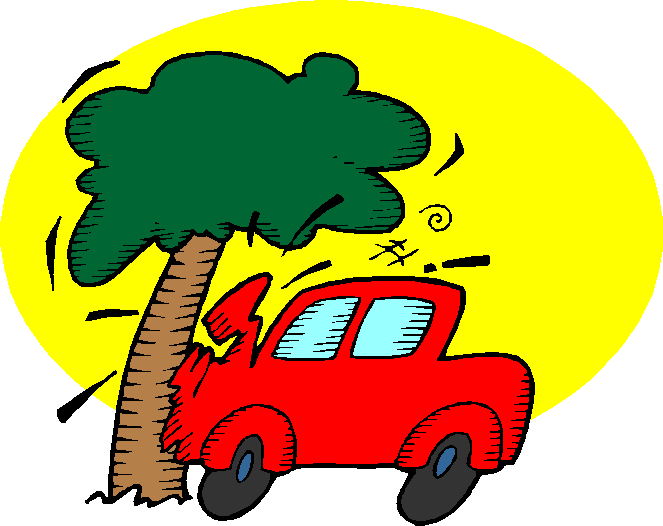
\includegraphics[width=1.75in]{../graphics/a2Homework-img1}
%%  \vspace{\stretch1}
  
\item In a crash test, a car strikes a wall with an average force of 
  \SI{1.23e7}{\newton} [S] over an interval of \SI{21.0}{\milli\second}.
  Calculate the impulse the car exerts on the wall.
  
\item In a crash test similar to the one described in the last problem, another
  car, with the same mass and velocity as the first car, experiences an impulse
  identical to the value you calculated in the last problem. However, the
  second car is designed to crumple more slowly than the first. As a result,
  the duration of the crash is \SI{57.1}{\milli\second}. Determine the average
  force the wall exerted on the second car.
  
\item A \SI{1385}{\kilo\gram} cannon containing a \SI{58.5}{\kilo\gram} cannon
  ball is on wheels. The cannon fires the cannon ball, giving it a velocity of
  \SI{49.8}{\metre\per\second} [N]. What is the initial velocity of the cannon
  the instant after it fires the cannon ball?
 
\item Two amusement park bumper cars are heading directly towards each other.
  The combined mass of car A plus driver is \SI{375}{\kilo\gram} and it is
  moving with a velocity of $+$\SI{1.8}{\metre\per\second}. The combined mass
  of car B plus driver is \SI{422}{\kilo\gram} and it is moving with a velocity
  of \SI{-1.4}{\metre\per\second}. When they collide, they become stuck
  together and continue moving along the same straight line. What is their
  velocity immediately after they collide?

%  \item An \SI{80}{\kilo\gram} astronaut has become detached from the
%  safety line connecting her to the International Space Station. She is
%  \SI{200}{\metre} from the station, and at rest relative to it. She only has
%  4.0 minutes of air remaining. To get herself back, she tosses a
%  \SI{10}{\kilo\gram} tool kit away from the station at
%  \SI{8.0}{\metre\per\second}. Will she make it back in time?
%  \vspace{\stretch1}
%  \newpage
%  
%  \item A \SI{2.0}{\kilo\gram} box is initially moving at
%  $+$\SI{3.0}{\metre\per\second} and is pushed along a horizontal, frictionless
%  surface with a net force $F$ that varies with time according to the following
%  graph:
%  \begin{center}
%    \begin{tikzpicture}[yscale=.14]
%      \foreach\x in {1,...,7} \draw(\x,1)--(\x,-1) node[below]{$\x$};
%      \foreach\y in {-10,-5,...,20}{
%        \draw[thin,gray!50] (7.5,\y)--(-.1,\y) node[left,black]{$\y$};
%      }
%      \draw[axes] (0,0)--(7.5,0) node[right]{$t$ (s)};
%      \draw[axes] (0,-13)--(0,25) node[above]{$F$ (N)};
%      \draw[ultra thick] (0,20)--(1,20)--(3,0)--(4,0)--(5,-10)--(7,-10);
%    \end{tikzpicture}
%  \end{center}
%  \begin{enumerate}[itemsep=3pt]
%    \item In the table below, indicate the momentum change of the box during
%    each second of elapsed time.
%    \begin{center}
%      {\large
%        \begin{tabular}{c|c}
%          Time (s) & Impulse (\si{\newton\second}) \\\hline
%          $0-1$ &\\
%          $1-2$ &\\
%          $2-3$ &\\
%          $3-4$ &\\
%        \end{tabular}
%        \hspace{.7in}
%         \begin{tabular}{c|c}
%          Time (s) & Impulse (\si{\newton\second}) \\\hline
%          $4-5$ &\\
%          $5-6$ &\\
%          $6-7$ &\\
%           & 
%        \end{tabular}
%      }
%    \end{center}
%
%    \item Plot the velocity vs.\ time graph for this motion in the space below.
%    Label all relevant quantities on the $x$ and $y$ axis.
%    \begin{center}
%      \begin{tikzpicture}[scale=.8]
%        \draw[gray!40] grid (7,8);
%        \draw[axes] (0,0)--(0,8.5) node[above]{$v$ (\si{\metre\per\second})};
%        \draw[axes] (0,0)--(7.5,0) node[right]{$t$ (\si\second)};
%      \end{tikzpicture}
%    \end{center}
%    \item At $t=\SI{7.0}\second$, the box collides with a wall and bounces
%    backwards at \SI{6.0}{\metre\per\second}. Given that the box is in contact
%    with the wall for \SI{.20}\second, calculate the average force that the
%    wall exerts on the box.
%
%  \end{enumerate}
%  \newpage
%  
%%  \item A billiard ball of mass \SI{0.155}{\kilo\gram} (``cue ball'') moves
%%  with a velocity of \SI{12.5}{\metre\per\second} towards a stationary billiard
%%  ball (``eight ball'') of identical mass and strikes it with a glancing blow.
%%  The cue ball moves off at an angle of \ang{29.7} clockwise from its original
%%  direction, with a speed of \SI{9.56}{\metre\per\second}.
%%  \begin{enumerate}[itemsep=3pt]
%%    \item What is the velocity of the eight ball?
%%    \item Determine whether the collision was elastic.
%%  \end{enumerate}
  
\item A \SI{1875}{\kilo\gram} car is travelling along a country road when the
  driver sees a deer dart out onto the road. The driver slams on the brakes
  and manages to stop before hitting the deer. The driver of a second car (mass
  \SI{2135}{\kilo\gram}) is driving too close. When the driver realizes that
  the car ahead has stopped, he hits the brakes but is unable to stop. The two
  cars lock together and skid another \SI{4.58}{\metre} along a straight line
  before coming to a stop. If the coefficient of friction between concrete and
  rubber is 0.750, what is the speed of the second car when it hits the stopped
  car?

\item While playing a game of billiards, your \SI{.17}{\kilo\gram} cue ball,
  travelling at \SI{1.9}{\metre\per\second}, glances off a stationary
  \SI{.16}{\kilo\gram} ``eight ball'' so that the eight ball moves off at
  \SI{1.3}{\metre\per\second} at an angle of \ang{32} clockwise from the cue
  ball's original path.
  \begin{enumerate}[itemsep=3pt]
  \item What is the final velocity (both magnitude and direction) of the cue
    ball?
  \item Calculate the total kinetic energy before and after the collision. Is
    the collision elastic?
  \end{enumerate}

%  \item Two blocks are free to slide along the frictionless wooden track
%  shown below. The block of mass $m_1=\SI{4.98}{\kilo\gram}$ is released from
%  the position shown, at height $h=\SI{5.00}\metre$ above the flat part of the
%  track. Protruding from its front end is the north pole of a strong magnet,
%  which repels the north pole of an identical magnet embedded in the back end
%  of the block of mass $m_2=\SI{9.40}{\kilo\gram}$, initially at rest. The two
%  blocks never touch.
%  \begin{center}
%    \begin{tikzpicture}
%      \draw[thick,fill=brown!50] (0,0)--(0,4)--(1,4)--(1,3.5) to[out=270,in=180]
%      (5,.5)--(12,.5)--(12,0)--(0,0);
%      \draw[thick,dashed] (.2,.5)--(5,.5);
%      \draw[thick,dashed] (.2,3.5)--(1,3.5);
%      \draw[<->,thick] (.5,.5)--(.5,3.5) node[midway,fill=brown!50]{$h$};
%      \draw[mass] (5.2,.5) rectangle (5.8,.9) node[right=-1]{$m_2$};
%      \draw[mass] (1,4) rectangle (1.4,3.5)
%      node[right=0]{$m_1$};
%    \end{tikzpicture}
%  \end{center}
%  Calculate:
%  \begin{enumerate}[itemsep=3pt]
%    \item The speed of $m_1$ just before the collision
%    \item The velocities of $m_1$ and $m_2$ after the elastic collision
%    \item The maximum height to which $m_1$ rises after the elastic collision
%  \end{enumerate}
\end{enumerate}



%\documentclass[12pt,compress,aspectratio=169]{beamer}
%\input{../mybeamer}
%
\chapter{Centre of Mass}
\label{chapter:cm}

%{Centre of Mass}
%  Finding an object's centre of mass is important, because
%  \begin{itemize}
%  \item The laws of motion are formulated by treating an objects as point
%    masses (for real-life objects, we let the forces apply to the centre of
%    mass)
%  \item Objects can have \emph{rotational} motion in addition to
%    \emph{translational} motion as well (we will examine that a bit more in a
%    very-important topic later)
%  \end{itemize}
%\end{frame}
%
%
%
\section{Centre of Mass: Definition}
The \textbf{centre of mass} (``CM'') is the \emph{weighted average} of the
masses in a system. The ``system'' may be:
\begin{itemize}
\item A collection of individual particles
\item A continuous distribution of mass with constant density. In this case,
  CM is also the geometric centre (\textbf{centroid}) of the object
\item A continuous distribution of mass with varying density
\item If the masses are inside of a \emph{uniform} gravitational
  field\footnote{See discussion on gravitational field in the first part of
  this class}, then the CM is also its \textbf{centre of gravity} (``CG'')
\end{itemize}




\section{Finding the Centre of Mass}

%{Simple Example}
%  Two equal masses $m$ along the $x$-axis, located at $x_1$ and $x_2$. Where is
%  the centre of mass of the system?
%  \begin{center}
%    \begin{tikzpicture}
%      \draw[axes] (-1,0)--(8,0) node[right]{$x$};
%      \draw[mass] (2,0) circle (.2) node{$m$};
%      \draw[mass] (6,0) circle (.2) node{$m$};
%      \draw[thick] (0,.85)--(0,-.45) node[below]{$O$};
%      \fill (4,0) circle (.05) node[above]{cm};
%      \begin{scope}[very thick,->|]
%        \draw (0,.35)--(2,.35) node[pos=0,left]{$x_1$};
%        \draw (0,.75)--(6,.75) node[pos=0,left]{$x_2$};
%        \draw[violet] (0,-.3)--(4,-.3) node[pos=0,left]{$x_\text{cm}$};
%      \end{scope}
%    \end{tikzpicture}
%  \end{center}
%  The centre of mass is at the half-way point between the masses:
%
%  \eq{-.1in}{
%    x_\text{cm}=\frac{x_1+x_2}2
%    \quad\quad\text{or}\quad\quad
%    x_\text{cm}=\frac{mx_1+mx_2}{2m}
%  }

%
%
%
%{Slightly More Challenging}
%  What if one of the masses are increased to $2m$? This is still not a
%  difficult problem; you can still \emph{guess} the right answer without
%  knowing the equation for center of mass. 
%  \begin{center}
%    \begin{tikzpicture}
%      \draw[axes] (-4,0)--(4,0) node[right]{$x$};
%      \draw[mass] (-2.5,0) circle (.3) node{$m$};
%      \draw[mass] (2.5,0) circle (.42) node{$2m$};
%      \fill (5/6,0) circle (.05) node[below]{cm};
%    \end{tikzpicture}
%  \end{center}
%  The answer is still simple. The centre of mass is no longer half way between
%  the two masses, but now $\frac13$ the total distance from the larger masses.
%  We can show using a weighted average:
%  
%  \eq{-.1in}{
%    x_\text{cm}=\frac{mx_1+(2m)x_2}{m+2m}
%  }

%
%
%
%{Many Point Masses}
%  The weighted average concept can now be applied to cases when there are
%  masses in two or more dimensions:
%  \begin{center}
%    \begin{tikzpicture}
%      \draw[axes] (-3,0)--(3,0) node[right]{$x$};
%      \draw[axes] (0,-1.5)--(0,1.5) node[above]{$y$};
%      \draw[mass] (-1.3,1) circle (.4) node{$m_1$};
%      \draw[mass] (-1.5,-.5) circle (.3) node{$m_2$};
%      \draw[mass] (1,.3) circle (.25) node{$m_3$};
%      \draw[mass] (0,.3) circle (.2) node{$m_4$};
%      \draw[mass] (2,-1) circle (.25) node{$m_5$};
%    \end{tikzpicture}
%  \end{center}

%
%
%
%{Centre of Mass Equation}
%  For a discrete number of $N$ masses, the centre of mass is defined as the
%  weighted average of the positions of the masses:
%
%  \eq{-.1in}{
%    \boxed{\vec x_\text{cm}=\frac{\sum_{i=1}^N m_i\vec x_i}{\sum_{i=1}^N m_i}}
%  }
%  \begin{center}
%    \begin{tabular}{l|c|c}
%      \rowcolor{pink}
%      \textbf{Quantity} & \textbf{Symbol} & \textbf{SI Unit} \\ \hline
%      Position of centre of mass (vector) & $\vec x_\text{cm}$ & \si\metre \\
%      Position of point mass $i$ (vector) & $\vec x_i$ & \si\metre \\
%      Point mass $i$ & $m_i$ & \si{\kilo\gram}
%    \end{tabular}
%  \end{center}
%  In components:
%
%  \eq{-.1in}{
%    x_\text{cm}=\frac{\sum m_ix_i}{m_\text{tot}}\quad\quad
%    y_\text{cm}=\frac{\sum m_iy_i}{m_\text{tot}}\quad\quad
%    z_\text{cm}=\frac{\sum m_iz_i}{m_\text{tot}}
%  }

%
%
%
%{An Example}
%  \textbf{Example 1:} Consider the following masses and their coordinates
%  which make up a ``discrete mass'' rigid body''
%  \begin{align*}
%    m_1&=\SI{5.0}{\kg} &\vec x_1&=3\xxx-2\zzz\\
%    m_2&=\SI{10.0}{\kg}&\vec x_2&=-4\xxx+2\yyy+7\zzz\\
%    m_3&=\SI{1.0}{\kg}&\vec x_3&=10\xxx-17\yyy+10\zzz
%  \end{align*}
%  What are the coordinates for the centre of mass of this system?

%
%
%
%{Continuous Mass Distribution}
%  When the number of masses approaches infinity, this becomes a continuous
%  distribution of mass. Taking the limit of masses $N\rightarrow\infty$ gives
%  the \emph{integral form} of our equation:
%
%  \eq{-.1in}{
%    \vec x_\text{cm}=\frac{\int\vec xdm}{\int dm}}
%
%  Calculus is not part of the AP Physics 1 curriculum, so you are welcome to
%  skip this slide. But this calculation is part of AP Physics C, which is
%  calculus-based. 

%
%
%
%{Centroid}
%  For an object with a uniform mass distribution (i.e.\ constant density), the
%  centre of mass is also its geometric centre, called the \textbf{centroid}.
%  \begin{center}
%    \pic{.7}{eng130C9_11}
%  \end{center}
%  The locations of centroids can be found in most physics textbooks.

%
%
%
%{Compound Shapes}
%  For compound shapes, the centre of mass is the weighted average of the centre
%  of mass of each component. For example, for the T-beam below:
%  \begin{center}
%    \begin{tikzpicture}[scale=.7]
%      \draw[axes] (0,0)--(4.5,0) node[right]{$x$};
%      \draw[axes] (0,0)--(0,4.5) node[left]{$y$};
%      \draw[blue!70!black,mass] (0,4)--(4,4)--(4,3)--(2.5,3)
%      --(2.5,0)--(1.5,0)--(1.5,3)--(0,3)--(0,4);
%    \end{tikzpicture}
%    \hspace{.1in}
%    \begin{tikzpicture}[scale=.7]
%      \draw[lightgray,fill=gray!20,thick] (0,4)--(4,4)--(4,3)--(2.5,3)--(2.5,0)
%      --(1.5,0)--(1.5,3)--(0,3)--(0,4);
%      \draw[lightgray,dotted,thick] (1.5,3)--(2.5,3);
%      \draw[axes] (0,0)--(4.5,0) node[right]{$x$};
%      \draw[axes] (0,0)--(0,4.5) node[left]{$y$};
%      \fill[blue!70!black] (2,3.5) circle (.08) node[right]{$\vec x_1$};
%      \fill[blue!70!black] (2,1.5) circle (.08) node[right]{$\vec x_2$};
%    \end{tikzpicture}
%    \hspace{.1in}
%    \begin{tikzpicture}[scale=.7]
%      \draw[lightgray,thick] (0,4)--(4,4)--(4,3)--(2.5,3)
%      --(2.5,0)--(1.5,0)--(1.5,3)--(0,3)--(0,4);
%      \draw[axes] (0,0)--(4.5,0) node[right]{$x$};
%      \draw[axes] (0,0)--(0,4.5) node[left]{$y$};
%      \fill[blue!30] (2,3.5) circle (.08) node[right]{$\vec x_1$};
%      \fill[blue!30] (2,1.5) circle (.08) node[right]{$\vec x_2$};
%      \fill[red!70!black] (2,2.64) circle (.08) node[right]{$\vec x_\text{cm}$};
%    \end{tikzpicture}
%  \end{center}

%
%
%
%{Symmetric Configurations}
%  \begin{itemize}
%  \item Any plane of symmetry, mirror line, axis of rotation, point of inversion
%    \emph{must} contain the centre of mass.
%  \item Caveat: only works if the density distribution is also symmetric
%  \item Again: if density is uniform, CM is also geometric centre (centroid)
%  \end{itemize}

%
%
%
%{``Negative Mass''}{A Mathematical Trick}
%  \begin{itemize}
%  \item Where there is a ``hole'' in the geometry, treat it as having negative
%    mass density $-\sigma$ in that region.
%  \item Negative masses don't exist, so this is really just a trick.
%  \item\textbf{Example:} What is the centre of mass of this shape?
%    \begin{center}
%      \begin{tikzpicture}
%        \draw[thick,fill=lightgray] circle (2);
%        \draw[thick,fill=black!2] (0,1) circle (1);
%        \fill circle (.04);
%        \draw[axes] (0,0)--(-1.41,-1.41)node[midway,below]{$r$};
%        \fill (0,1) circle (.04);
%        \draw[axes] (0,1)--(.707,.293) node[right]{$r/2$};
%      \end{tikzpicture}
%    \end{center}
%  \end{itemize}

%
%
%
%{Negative Mass Example}
%  \begin{itemize}
%  \item This is how we would think of it:
%    \begin{center}
%      \begin{tikzpicture}[scale=.6]
%        \draw[thick,fill=lightgray] circle (2);
%        \draw[thick,fill=black!2] (0,1) circle (1);
%        \fill circle (.04);
%        \draw[axes] (0,0)--(-1.41,-1.41) node[midway,below]{$r$};
%        \fill (0,1) circle (.04);
%        \draw[axes] (0,1)--(.707,.293) node[right]{$r/2$};
%        \draw[thick,fill=lightgray] (6,0) circle (2) node{\large$A$};
%        \draw[thick] (11,1) circle (1) node{\large$B$};
%        \node at (3,0) {\huge=};
%        \node at (9,0) {\huge+};
%      \end{tikzpicture}
%    \end{center}
%  \item Let the origin of the coordinate system to located at the centre of $A$
%  \item Based on symmetry: $x_\text{cm}=0$; only have to find $y$-coordinate.
%  \end{itemize}
%
%  \eq{-.2in}{
%    y_\text{cm}
%    =\frac{\sum y_i m_i}{\sum m_i}
%    =\frac{m_A(0) + m_B (r/2)}{m_A+m_B}
%    =\frac{-\sigma\pi\left(r/2\right)^2(r/2)}
%    {\sigma\pi r^2-\sigma\pi\left(r/2\right)^2}
%    =\frac{-r}6
%  }

%
%
%
\section{Momentum and Centre of Mass}

\subsection{Velocity of the Centre of Mass}
Taking the change in the position of the CM ($\Delta\vec x_\text{cm}$) over a
finite time interval ($\Delta t$) gives the expression for $\vec v_\text{cm}$,
the average velocity of the centre of mass:
\begin{equation*}
  \vec v_\text{cm}
  =\frac{\color{magenta}\Delta\vec x_\text{cm}}{\Delta t}
  =\frac1{\Delta t}
  {\color{magenta}\left[\frac{\sum\Delta(m_i\vec x_i)}{\sum m_i}\right]}
  =\frac1{m_\text{tot}}
  \left[\sum m_i{\color{orange}\frac{\Delta\vec x_i}{\Delta t}}\right]
  =\frac1{m_\text{tot}}\sum m_i{\color{orange}\vec v_i}
\end{equation*}
The velocity of the centre of mass is the weighted sum of the velocities of
the discrete masses:
\begin{equation}
  \vec v_\text{cm} = \frac{\sum m_i\vec v_i}{m_\text{tot}}
\end{equation}
Like the expression for the position of the CM, the weight for the sum is the
individual masses.


\subsection{Velocity and Momentum}
We can rearrange the equation for the velocity of the centre of mass to relate
it to momentum, because the term $\sum m_i\vec v_i=\vec p_\text{net}$ is the net
momentum of \emph{all} the discrete masses:
\begin{equation}
  \vec v_\text{cm} = \frac{\sum m_i\vec v_i}{m_\text{tot}}
  \quad\longrightarrow\quad
  \vec p_\text{net}= \sum m_i\vec v_i = m_\text{tot}\vec v_\text{cm}
\end{equation}
During a collision, there is no change in the net momentum\footnote{Because
there are are no external forces}, the centre of mass will continue to move at
the same velocity before/after the collision, as if the collision never
occurred.

%
%
%
%{Centre of Mass During Collision}
%  \vspace{.1in}
%  During a collision\footnote{As we have studied in conservation of momentum in
%  Class 9}, there are no external forces, therefore the velocity of the CM
%  remains constant. Consider this perfectly inelastic collision in 1D  between
%  two masses:
\begin{figure}[ht]
  \centering
  \begin{tikzpicture}[scale=.8,thick]
    \begin{scope}[violet]
      \draw (1,0) rectangle (2,1) node[midway]{$m_1$};
      \draw (4,0) rectangle (5,1) node[midway]{$m_2$};
      \draw[vectors] (.8,1.3)--(2.5,1.3) node[right]{$v_1$};
      \draw[vectors] (4,1.3)--(5,1.3) node[right]{$v_2$};
      \node[above] at (3,1.5) {Before Collision};
    \end{scope}
    \draw[vectors] (2.7,.5)--(3.7,.5) node[above]{$v_\text{cm}$};
    \begin{scope}[orange]
      \draw (10,0) rectangle (11,1) node[midway]{$m_1$};
      \draw (11,0) rectangle (12,1) node[midway]{$m_2$};
      \draw[vectors] (10.2,1.3)--(11.8,1.3) node[right]{$v'$};
      \node[above] at (11,1.5) {After Collision};
    \end{scope}
    \draw (0,0)--(14,0);
    \draw (2.7,.5) circle (.15);
    \fill (2.7,.5)--(2.85,.5) arc(0:90:.15)--cycle;
    \fill (2.7,.5)--(2.55,.5) arc(180:270:.15)
    node[below=-2] (c){\scriptsize cm\par}--cycle; 
    
    \draw (11,.5) circle (.15);
    \fill (11,.5)--(11.15,.5) arc(0:90:.15)--cycle;
    \fill (11,.5)--(10.85,.5) arc(180:270:.15)
    node[below=-2] {\scriptsize cm\par}--cycle; 
    
    \node[text width=2.07in,draw,violet,below right] (a) at (-.5,-.6)
         {Using the definition of the velocity of the CM, we find
           that \emph{before} the collision, the CM moves at:
           \vspace{-.05in}
           \begin{displaymath}
             v_\text{cm} = \frac{\sum m_iv_i}{\sum m_i}
             =\frac{m_1v_1+m_2v_2}{m_1+m_2}
           \end{displaymath}\par
         };
         \draw[axes,violet] (a)--(c);
         
         \node[text width=2in,draw,orange,below left] at (14.5,-.6)
              {Using conservation of momentum, we find the final velocity
                \emph{after} the collision is the velocity of the CM:
                \vspace{-.05in}
                \begin{displaymath}
                  v'=\frac{m_1v_1+m_2v_2}{m_1+m_2}=v_\text{cm}
                \end{displaymath}
                %\vspace{-.08in}It is the same as $v_\text{cm}$ before the
                %collision!
                \par
              };
  \end{tikzpicture}
\end{figure}


\section{Acceleration of the Centre of Mass}
Finding the rate of change of the net momentum (i.e\ applying the 2nd law of
motion to this collection of masses):
%  
%  \eq{-.1in}{
%    \frac{\Delta\vec p_\text{net}}{\Delta t}=
%    \frac{\Delta(m\vec v_\text{cm})}{\Delta t}
%  }
%
%  If the system mass is constant, then this equation reduces to:
%
%  \eq{-.1in}{
%    \frac{\Delta\vec p_\text{net}}{\Delta t}
%    =m\frac{\Delta\vec v_\text{cm}}{\Delta t}
%    \quad\longrightarrow\quad
%    \boxed{
%      \vec F_\text{net}=m\vec a_\text{cm}
%    }
%  }
%  
%  We can see that when a net force is applied to an object, the object's
%  acceleration is evaluated at the centre of mass.

%
%
%%{What This All Means}
%%  \begin{itemize}
%%  \item Newton was right all along by treating all objects as point masses
%%    located at the CM
%%  \end{itemize}


\part{Periodic Motion}

\chapter{Circular Motion}
\label{chapter:circ-motion}

The \textbf{circular motion} (Fig.~\ref{fig:circ-motion1}) is the simplest
form of curvilinear motions, an object of mass $m$ moves in a circular path
about a fixed centre.
Like we did in Chapters~\ref{chapter:kinematics} and \ref{chapter:dynamics},
we will begin studying the circular motion, first be defining the coordinate
system, and then to the kinematic quantities, and then onto dynamics.

\section{Polar Coordinates}
In the majority of two-dimensional motion, 
%discussed in earlier chapters,
it is usually the most convenient to describe an object's position using the
Cartesian coordinate system, i.e.\ using the $x$ and $y$ coordinates as
functions of time:
\begin{equation}
  \mathbf r(t)=x(t)\hat x + y(t)\hat y
\end{equation}
However, for circular motion or general \textbf{curvilinear motions}, the
\textbf{polar coordinate system} is preferred. The position of an object is
described by:
\begin{equation}
  \mathbf r(t)=r(t)\hat{\bm r} + \theta(t)\hat{\bm\theta}
\end{equation}
where $r(t)$ is distance from the origin, and $\theta(t)$ is the standard
angle, measured counterclockwise from the $x$ axis. Some examples of
curvilinear motion are shown in Fig.~\ref{fig:curvilinear-motions}.

It is clear from basic geometry that Cartesian and polar coordinates are
related by:
\begin{align*}
  x(t)&=r(t)\cos\left(\theta(t)\right)\\
  y(t)&=r(t)\sin\left(\theta(t)\right)
\end{align*}

\begin{figure}[ht]
  \centering
  \begin{subfigure}{.2\linewidth}
    \centering
    \begin{tikzpicture}[scale=.9]
      \draw[axes] (-2,0)--(2,0) node[right]{$x$};
      \draw[axes] (0,-2)--(0,2) node[above]{$y$};
      \draw[function] circle (1.5);
    \end{tikzpicture}
    \caption{Circular motion}
    \label{fig:circ-motion1}
  \end{subfigure}  
  \begin{subfigure}{.2\linewidth}
    \centering
    \begin{tikzpicture}[scale=.9]
      \draw[axes] (-2,0)--(2,0) node[right]{$x$};
      \draw[axes] (0,-2)--(0,2) node[above]{$y$};
      \draw[function,rotate=30] ellipse (1.8 and 1);
    \end{tikzpicture}
    \caption{Elliptical motion}
  \end{subfigure}
  %\begin{subfigure}{.2\linewidth}
  %  \centering
  %  \begin{tikzpicture}[scale=.9]
  %    \draw[axes] (-2,0)--(2,0) node[right]{$x$};
  %    \draw[axes] (0,-2)--(0,2) node[above]{$y$};
  %    \draw[function,domain={-1.7:1.7}] plot(\x,{.5*(\x*\x)-.3});
  %  \end{tikzpicture}
  %  \caption{Parabolic motion}
  %\end{subfigure}
  %\begin{subfigure}{.2\linewidth}
  %  \centering
  %  \begin{tikzpicture}[scale=.9]
  %    \draw[axes] (-2,0)--(2,0) node[right]{$x$};
  %    \draw[axes] (0,-2)--(0,2) node[above]{$y$};
  %    \draw[domain=0:25,variable=\t,samples=200,function]
  %    plot({\t r:1.75*exp(-.1*\t)});
  %  \end{tikzpicture}
  %  \caption{Inward/Outward spiral}
  %s\end{subfigure}
  \caption{Examples of curvilinear motion in two dimensions}
  \label{fig:curvilinear-motions}
\end{figure}

%Like the Cartesian system, the polar coordinate system is also right-handed;
%TML%basics vectors $\hat{\bm r}$ (``radial direction'') and $\hat{\bm\theta}$
%TML%(``angular direction'') point in the directions shown in
%TML%Fig.~\ref{fig:basis-vecs},
%TML%\begin{figure}[ht]
%TML%  \centering
%TML%  \begin{tikzpicture}[scale=.75]
%TML%    \draw[axes] (-3,0)--(3,0) node[right]{$x$};
%TML%    \draw[axes] (0,-3)--(0,3) node[above]{$y$};
%TML%    \draw[vector] (0,0)--(1,0) node[below]{$\iii$};
%TML%    \draw[vector] (0,0)--(0,1) node[left] {$\jjj$};
%TML%    \draw circle (2.5);
%TML%    \begin{scope}[rotate=38]
%TML%      \draw[vector] (0,0)--(2.45,0) node[midway,above]{$r$};
%TML%      \draw[vector] (2.5,0)--(3.5,0) node[right]{$\hat r$};
%TML%      \draw[vector] (2.5,0)--(2.5,1) node[above]{$\hat\theta$};
%TML%      \draw[mass] (2.5,0) circle (.1);
%TML%    \end{scope}
%TML%    \draw[axes] (1.5,0) arc (0:38:1.5) node[pos=.55,right]{$\theta$};
%TML%  \end{tikzpicture}
%TML%  \caption{Basis vectors for rectilinear and curvilinear motions}
%TML%  \label{fig:basis-vecs}
%TML%\end{figure}
  %TML%and rotate as the object moves.

%TML%%\section{Cylindrical Coordinates in 3D}
%TML%%
%TML%%One way to extend the coordinates coordinate system into 3D is the
%TML%%\textbf{cylindrical coordinate system}. Note that the discussions for this
%TML%%topic focuses on $xy$ plane. Since the $z$-axis is linearly independent of
%TML%%the $xy$ plane, motion along that direction is independent.
%TML%%
%TML%%\begin{figure}[ht]
%TML%%  \centering
%TML%%  \begin{tikzpicture}[scale=.75]
%TML%%    \draw[axes] (0,0)--(-2.5,-2.5) node[below]{$x$};
%TML%%    \draw[axes] (0,0)--(5,0) node[right]{$y$};
%TML%%    \draw[axes] (0,0)--(0,5) node[above]{$z$};
%TML%%    \draw[axes] (-1,-1) arc (-110:-45:2) node[midway,below]{$\theta$};
%TML%%    \draw[dashed,fill=green!40,opacity=.4](0,0)--(3,-1.5)
%TML%%    node[pos=.6,below left,opacity=1]{$r$}--(3,2.5)
%TML%%    node[midway,right,black,opacity=1]{$z$}--(0,4);
%TML%%    \fill (3,2.5) circle(.1) node[right]{$\bm r(r,\theta,z)$};
%TML%%  \end{tikzpicture}
%TML%%\end{figure}
%TML%
%TML%
\section{Kinematics of Circular Motion}
The kinematics of circular motion is similar to that of the one-dimensional
kinematics. There is a positive direction, and a negative direction. From the
context of the $xy$-plane, the positive direction is counterclockwise---as it
is standard in mathematics---and the negative direction is clockwise. The
origin of the coordinate system is where the circular path intersects the
$x$-axis. However, unlike in rectilinear 1D motion, objects moving in one
direction along a circular path will return to the origin.

\subsection{Angular Position}

\textbf{Angular position} $\theta(t)$ is the location of an object along the
circular path at a distance $r$ from the origin. The angle is measured in
\emph{radians}. In the context of the Cartesian $xy$-plane, $\theta$ measured
from the $+x$-axis. This angle is positive if it is measured counter-clockwise
from the axis, and negative if measured clockwise. In the example shown in
Fig.~\ref{fig:angular-position}, the angular position of object A is positive,
while the angular position of object B is negative. If an object is in circular
motion, angular position is a continuous function of time. (At this time, we
are not concerned with what kind of function this is; it only means that the
object can be at one position at any given time.)
\begin{figure}[ht]
  \centering
  \begin{tikzpicture}[scale=.7]
    \draw[axes] (-3,0)--(3,0) node[right]{$x$};
    \draw[axes] (0,-3)--(0,3) node[above]{$y$};
    \draw[gray] circle (2.5);
    \begin{scope}[rotate=138]
      %\draw[vector] (0,0)--(2.44,0) node[midway,above]{$\bm r_A$};
      \draw[mass] (2.5,0) circle (.08) node[above]{$A$};
    \end{scope}
    \draw[vector] (2.5,0) arc (0:138:2.5) node[midway,above]{$\theta_A>0$};
    \begin{scope}[rotate=-65]
      %\draw[vector] (0,0)--(2.44,0) node[midway,right]{$\bm r_A$};
      \draw[mass] (2.5,0) circle (.08) node[above]{$B$};
    \end{scope}
    \draw[vector] (2.5,0) arc (0:-65:2.5) node[midway,right]{$\theta_B<0$};
  \end{tikzpicture}
  \caption{Angular position of two objects along the $xy$-plane.}
  \label{fig:angular-position}
\end{figure}

For the remainder of the chapter, the angular position of an object is not
particular important, because
\begin{itemize}
\item The $x$-axis can be defined arbitrarily
\item There are multiple ways
\end{itemize}
Instead we will focus on the other related kinematic quantities in circular
motion: angular displacement, angular velocity and angular acceleration.


\subsection{Angular Displacement}
If the object is moving along this circular path, then the change in the
angular position is the object's \textbf{angular displacement}
$\Delta\theta(t)$. It is defined as the difference between an object's current
angular position $\theta(t)$ and its initial angular position $\theta_i$:
%For constant distance $r$ to the origin, the \textbf{angular position}
%$\theta$ determines an object's position as a continuous function of
%time, i.e.:
%%\footnote{The more mathematically rigorous notation is to express the
%%angular position as a vector along the angular direction:
%%\begin{displaymath}
%%  \bm\theta=\theta(t)\hat{\bm\theta}
%%\end{displaymath}
%%The magnitude is $\theta(t)$ and the direction is $\hat{\bm\theta}$.}:
%\begin{equation}
%  \boxed{
%    \theta=\theta(t)
%  }
%  \label{eq:angular-position}
%\end{equation}
%The unit for angular position is a \emph{radian} (rad): If motion is confined
%to the $xy$-plane, then $\theta$ is the standard angle: $\theta$ is positive
%when measured counterclockwise from the $x$-axis, and negative when it is
%measured clockwise.
%
%When an object moves along this circular path, we can calculate the change in
%the angular position (i.e.\ change in the angle). This is the object's
%\textbf{angular displacement} $\Delta\theta$:
\begin{equation}
  \boxed{
    \Delta\theta(t)=\theta(t)-\theta_i
  }
  \label{eq:angular-displacement}
\end{equation}
Like angular position, $\Delta\theta$ is positive if the object moves
counterclockwise, and negative if it moves clockwise, as shown in
Fig.~\ref{fig:angular-displacement}. Angular displacement is also measured in
\emph{radians}.

%At this point, it should be obvious that angular position and
%angular displacemnet are analogous to the equations one-dimensional position
%and displacement presented in Chapter~\ref{chapter:kinematics}.
\begin{figure}[ht]
  \centering
  \begin{tikzpicture}[scale=.7]
    \draw[axes] (-3,0)--(3,0) node[right]{$x$};
    \draw[axes] (0,-3)--(0,3) node[above]{$y$};
    \draw circle (2.5);

    \draw[axes,rotate=35] (2.5,0) arc (0:95:2.5)
    node[midway,right=5]{$\Delta\theta>0$};
    \draw[fill=lightgray,rotate=35] (2.5,0) circle (.1);
    \draw[mass,rotate=130] (2.5,0) circle (.1);

    \draw[axes,rotate=10] (2.5,0) arc (0:-70:2.5)
    node[midway,right]{$\Delta\theta<0$};
    \draw[fill=lightgray,rotate=10] (2.5,0) circle (.1);
    \draw[mass,rotate=-60] (2.5,0) circle (.1);
  \end{tikzpicture}
  \caption{Positive and negative angular displacement}
  \label{fig:angular-displacement}
\end{figure}

\subsection{Angular Velocity}
Analogous to the relationship between position and velocity in rectilinear
motions, for circular motion, \textbf{angular velocity} (or
\textbf{angular frequency}) $\omega(t)$ is the rate of change of angular
position, i.e.\ how quickly angular position changes with time. We can define
the \textbf{average angular velocity} as the angular displacement over a
finite time interval:
%$\omega_\text{avg}(t)$, is the time derivative of the angular position,
%measured in \emph{radian per second} (\si{\radian\per\second}). It is also a
%function of time:
\begin{equation}
  \boxed{
    \omega_\text{avg}(t)=\frac{\Delta\theta}{\Delta t}
    =\frac{\theta(t)-\theta_i}{t-t_0}
  }
\end{equation}
When the time interval approaches zero ($\Delta t\rightarrow 0$), we have the
\textbf{instantaneous angular velocity} $\omega(t)$ at time $t$. Both average
and instantaneous velocities are continous functions of time.

Again, if motion is confined to the $xy$-plane, then $\omega$ is positive when
the object moves in the counterclockwise direction, and negative when it moves
clockwise (Fig.~\ref{fig:omega-plus-minus}).
\begin{figure}[ht]
  \centering
  \begin{tikzpicture}[scale=.75]
    \draw[axes] (-3,0)--(3,0) node[right]{$x$};
    \draw[axes] (0,-3)--(0,3) node[above]{$y$};
    \draw[axes] (1,0) arc (0:38:1) node[midway,right]{$\theta$};
    \draw circle (2.5);
    \begin{scope}[rotate=38]
      \draw[thick] (0,0)--(2.44,0) node[midway,above]{$r$};
      \draw[vector] (2.5,.08)--(2.5,1.5) node[above]{$\bm v$};
      \draw[mass] (2.5,0) circle (.1);
    \end{scope}
  \end{tikzpicture}
  \caption{Sign convention for $\omega$ and direction of velocity vector
    $\bm v$ when circular motion is confined to the $xy$-plane}
  \label{fig:omega-plus-minus}
\end{figure}



\subsection{Velocity and Speed}
As the object moves with angular speed $\omega$, the actual velocity vector
$\bm v$ is tangent to the circle. Obviously
$\bm v$ is not constant in time, as its direction is always changing.
However, there is a simple mathematical relationship between the speed of object
$v(t)=|\bm v(t)|$ and the angular speed $|\omega|$:
\begin{equation}
  \boxed{
    v=r|\omega|
  }
\end{equation}
\begin{remark}
  For your information, the velocity vector $\bm v$ along \emph{any} path
  is \emph{always} tangent to the path. This should be obvious when you
  consider a car being driven on a highway.
\end{remark}

%\begin{itemize}
%\item The direction of $\bm v$ is tangent to circle, along
%  $\hat\theta$, and therefore $\perp$ to $\hat r$
%\item If $\omega>0$, the motion is counter-clockwise
%\item If $\omega<0$, the motion is clockwise
%\end{itemize}
  
%    \begin{tikzpicture}[scale=.75]
%      \draw[axes] (-3,0)--(3,0) node[right]{$x$};
%      \draw[axes] (0,-3)--(0,3) node[above]{$y$};
%      \draw[axes] (1,0) arc (0:38:1) node[midway,right]{$\theta$};
%      \draw circle (2.5);
%      \begin{scope}[rotate=38]
%        \draw[vector] (0,0)--(2.44,0) node[midway,above]{$\bm r$};
%        \draw[vector] (2.5,.08)--(2.5,1.5) node[above]{$\bm v$};
%        \draw[mass] (2.5,0) circle (.1);
%      \end{scope}
%    \end{tikzpicture}

%The velocity of the object in circular motion is more properly related to
%the angular velocity using this vector cross product:
%\begin{equation}
%  \bm v=\bm\omega\times\bm r
%\end{equation}
%$\bm\omega$ is out of the page if motion is counterclockwise, and into the page
%if motion is clockwise. Visualizing $\bm\omega$ takes practice, but this vector
%notation is mathematically rigorous and consistent
%  
%
%
%
%
%%\begin{frame}{Relativity Velocity}
%%  If two points $A$ and $B$ are rotating with the same angular velocity with the
%%  same cent, their relative position is given by:
%%
%%  \begin{equation}
%%    \boxed{
%%      \bm V_B=\bm V_A+ \bm\omega\times\bm r_{BA}
%%    }
%%  }
%%
%%  Where $\bm r_{BA}$ is the position of $B$ relative to $A$.


\subsection{Angular Acceleration and Tangential Acceleration}
Analogous to the relation between velocity $\bm v$ and acceleration
$\bm a$, \textbf{angular acceleration} $\alpha$ is the rate of change of
angular velocity, i.e.\ how quickly angular velocity changes with time:
\begin{equation}
  \boxed{
    \alpha_\text{avg}(t)=\frac{\Delta\omega(t)}{\Delta t}
    =\frac{\omega(t)-\omega_i}{t-t_0}
  }
\end{equation}
The unit for angular acceleration is \emph{radian per second squared}
\si{\radian\per\second\squared}.
%The sign convention for $\alpha$ is the same
%as for $\theta$ and $\omega$.
Similar to the relationship between velocity and angular velocity,
\textbf{tangential acceleration} $a_t$ along the direction of motion is related
to angular acceleration $\alpha$ by the radius $r$:
\begin{equation}
  \boxed{
    |\bm a_t(t)|=r|\alpha|
  }
\end{equation}
For \emph{uniform} circular motion, $\omega$ is constant, and therefore
$\bm a_t=0$.

%By the fundamental theorem of calculus, we can of course integrate angular
%acceleration to find the angular velocity (or the \emph{change} in angular
%velocity) as a function of time:
%\begin{equation}
%  \boxed{
%    \omega(t)=\int\alpha(t)\dl t+\omega_0
%  }
%  \quad\quad
%  \boxed{
%    \Delta\omega(t)=\int_{t_0}^t\alpha(t)\dl t
%  }
%\end{equation}
%The relationships are the same as in rectilinear motion.
%
%
%
\subsection{Period \& Frequency}
%%    \begin{tikzpicture}[scale=.75]
%%      \draw[axes] (-3,0)--(3,0) node[right]{$x$};
%%      \draw[axes] (0,-3)--(0,3) node[above]{$y$};
%%      \draw[axes] (1,0) arc (0:38:1) node[midway,right]{$\theta$};
%%      \draw circle (2.5);
%%      \begin{scope}[rotate=38]
%%        \draw[vector] (0,0)--(2.44,0) node[midway,above]{$\bm r$};
%%        \draw[vector] (2.5,.08)--(2.5,1.5) node[above]{$\bm v$};
%%        \draw[mass] (2.5,0) circle (.1);
%%      \end{scope}
%%    \end{tikzpicture}
For constant angular velocity $\omega$ (uniform circular motion), the motion
is strictly periodic. Its \textbf{frequency} and \textbf{period} are given by:
\begin{equation}
  \boxed{ f=\frac\omega{2\pi} }\quad\quad
  \boxed{ T=\frac{2\pi}\omega}\quad\quad
  \boxed{ f=\frac1T}
\end{equation}
Period $T$ is measured in \emph{seconds} (\si\second) and frequency $f$ is
measured in \textbf{hertz} (\si\hertz).
  



\subsection{Kinematic Equations for Circular Motion}
For \emph{constant} angular acceleration $\alpha$, the kinematic equations are
the same as in rectilinear motion, but with $\theta$ replacing $x$, $\omega$
replacing $v$, and $\alpha$ replacing $a$:
\begin{align}
  \Delta\theta &= \omega_i t + \frac12\alpha t^2\\
  \Delta\theta &= \omega_f t + \frac12\alpha t^2\\
  \Delta\theta &=\frac{\theta_i+\theta_f}2 \\
  \omega_f &=\omega_i + \alpha t\\
  \omega_f^2& = \omega_0^2+ 2\alpha\Delta\theta
\end{align}
For non-constant $\alpha$, calculus will be required.




%  \textbf{Example:} An object moves in a circle with angular acceleration
%  \SI{3.0}{\radian\per\second\squared}. The radius is \SI{2.0}{\metre} and it
%  starts from rest. How long does it take for this object to finish a circle?



\subsection{Centripetal Acceleration}% \& Centripetal Force}
Even when there is no angular acceleration, there is also a component of
acceleration towards the centre of the motion,
%\begin{figure}[ht]
%  \centering
%  \begin{tikzpicture}
%    \draw[->](-3,0)--(3,0);
%    \draw[->](0,-3)--(0,3);
%    \draw circle (2.5);
%    \begin{scope}[rotate=30]
%      \draw[->,very thick,blue](2.5,0)--(2.5,1.5) node[above]{$\bm v_i$};
%      \draw[->,very thick,red] (0,0)--(2.5,0)node[pos=.6,below]{$\bm r_i$};
%      \fill (2.5,0) circle(.06);
%    \end{scope}
%    \begin{scope}[rotate=90]
%      \draw[->,very thick,blue] (2.5,0)--(2.5,1.5)node[left]{$\bm v_f$};
%      \draw[->,very thick,red] (0,0)--(2.5,0) node[midway,left]{$\bm r_f$};
%TML%%      \fill (2.5,0) circle(.06);
%TML%%    \end{scope}
%TML%%    \draw(0,1)[<->] arc(90:30:1) node[pos=.6,above]{$\Delta\theta$};
%TML%%  \end{tikzpicture}
%TML%%\end{figure}
%TML%called the \textbf{centripetal acceleration} $\bm a_c$.
%TML%%\begin{equation}
%TML%%  \boxed{
%TML%%    \bm a_c=-\frac{v^2}r\hat{\bm r}=-(\omega^2r)\hat{\bm r}
%TML%%  }
%TML%%\end{equation}
%TML%%The negative sign indicates that the direction of $\bm a_c$ %and $\bm F_c$ are
%TML%%is radially \emph{inward}, towards the centre of motion, as $\hat{\bm r}$ is
%TML%%the outward radial direction. In uniform circular motion ($\alpha=0$), where
%TML%%the period or frequency are known, the speed of the object is:
%TML%%\begin{equation}
%TML%%  v=\omega r = 2\pi rf = \frac{2\pi r}T
%TML%%\end{equation}
%TML%%Centripetal acceleration can therefore be expressed based on $T$ or $f$:
%TML%%\begin{equation}
%TML%%  \bm a_c=-(\omega^2r)\hat{\bm r}\quad\rightarrow\quad
%TML%%  \boxed{
%TML%%    \bm a_c=-\frac{4\pi^2r}{T^2}\hat{\bm r}=-4\pi^2rf^2\hat{\bm r}
%TML%%  }
%TML%%\end{equation}
%TML%
%TML%Consider an object in uniform circular motion in the counterclockwise
%TML%direction with constant radius $r$ and constant speed $v$ (i.e.\ constant
%TML%angular speed $\omega=v/r$), as shown in
%TML%Fig.~\ref{fig:v-in-uniform-circ-motion}. At initial time $t_0$, the position
%TML%and velocity of the object are given by $\bm r_0=\bm r(t_0)$ and
%TML%$\bm v_0=\bm v(t_0)$. Then, at a later time $t_1=t_0+\Delta t$, the object has
%TML%moved through an angular displacement of $\Delta\theta$, and the final
%TML%position and velocity are now $\bm r_1=\bm r(t_1)$ and $\bm v_1=\bm v(t_1)$.
%TML%\begin{figure}[ht]
%TML%  \centering
%TML%  \begin{tikzpicture}
%TML%    \draw[axes] (-3,0)--(3,0);
%TML%    \draw[axes] (0,-3)--(0,3);
%TML%    \draw circle (2.5);
%TML%    \begin{scope}[rotate=30]
%TML%      \draw[vector,blue] (2.5,0)--(2.5,1.5) node[above]{$\bm v_0$};
%TML%      \draw[vector,red] (0,0)--(2.5,0) node[pos=.6,below]{$\bm r_0$};
%TML%      \fill (2.5,0) circle (.06);
%TML%    \end{scope}
%TML%    \begin{scope}[rotate=90]
%TML%      \draw[vector,blue] (2.5,0)--(2.5,1.5) node[left]{$\bm v_1$};
%TML%      \draw[vector,red] (0,0)--(2.5,0) node[midway,left]{$\bm r_1$};
%TML%      \fill (2.5,0) circle (.06);
%TML%    \end{scope}
%TML%    \draw[<-,thick] (0,1) arc (90:30:1) node[pos=.6,above]{$\Delta\theta$};
%TML%  \end{tikzpicture}
%TML%  \caption{An object in counter-clockwise uniform circular motion}
%TML%  \label{fig:v-in-uniform-circ-motion}
%TML%\end{figure}
%TML%
%TML%From the definition of acceleration,
%TML%\begin{equation}
%TML%  \bm a_c=\frac{\Delta\bm v}{\Delta t}=\frac{\bm v_1-\bm v_0}{\Delta t}
%TML%\end{equation}
%TML%And the magnitude of the centripetal acceleration is
%TML%\begin{equation}
%TML%  |\bm a_c|=\frac{|\Delta\bm v|}{\Delta t}
%TML%\end{equation}
%TML%Since $|\bm r_0|=|\bm r_i|=r$ (circular motion), and $|\bm v_0|=|\bm v_1|=v$
%TML%(constant speed, uniform circular motion), the triangles formed by the
%TML%displacement vector $\Delta\bm r$ and the change in velocity $\Delta\bm v$ are
%TML%similar isosceles triangles, as shown in Fig.~\ref{fig:sim-triangles}.
%TML%\begin{figure}[ht]
%TML%  \centering
%TML%  \begin{subfigure}{.4\linewidth}
%TML%    \centering
%TML%    \begin{tikzpicture}[scale=1.5,vector]
%TML%      \draw[rotate=-60,red] (0,0)--(0,2) node[midway,below]{$\bm r_0$};
%TML%      \draw[red] (0,0)--(0,2) node[midway,left]{$\bm r_1$};
%TML%      \draw (2*sin{60},1)--(0,2) node[midway,above]{$\Delta\bm r$};
%TML%      \draw[<-,thick] (0,.8) arc (90:30:.8) node[midway,above]{$\Delta\theta$};
%TML%    \end{tikzpicture}
%TML%    \caption{Displacement}
%TML%  \end{subfigure}
%TML%  \begin{subfigure}{.4\linewidth}
%TML%    \centering
%TML%    \begin{tikzpicture}[scale=1.5,vector]
%TML%      \draw[rotate=-60,blue] (0,0)--(-2,0) node[midway,right]{$\bm v_0$};
%TML%      \draw[blue](0,0)--(-2,0) node[midway,below]{$\bm v_1$};
%TML%      \draw(-1,2*sin{60})--(-2,0) node[midway,left]{$\Delta\bm v$};
%TML%    \end{tikzpicture}
%TML%    \caption{Change in velocity}
%TML%  \end{subfigure}
%TML%  \caption{Vector diagrams for change in position and velocity are similar
%TML%    isosceles triangles}
%TML%  \label{fig:sim-triangles}
%TML%\end{figure}
%TML%
%TML%
%TML%%\begin{tikzpicture}
%TML%%  \begin{scope}[very thick,->]
%TML%%    \draw[rotate=-60,red](0,0)--(0,2) node[midway,below]{$r$};
%TML%%    \draw[red](0,0)--(0,2) node[midway,left]{$r$};
%TML%%    \draw (2*sin{60},1)--(0,2)node[midway,above]{$|\Delta\bm r|$};
%TML%%  \end{scope}
%TML%%\end{tikzpicture}
%TML%%\begin{tikzpicture}
%TML%%  \begin{scope}[very thick,->]
%TML%%    \draw[rotate=-60,blue](0,0)--(-2,0) node[midway,right]{$v$};
%TML%%    \draw[blue](0,0)--(-2,0) node[midway,below]{$v$};
%TML%%    \draw(-1,2*sin{60})--(-2,0) node[midway,left]{$|\Delta\bm v|$};
%TML%%  \end{scope}
%TML%%\end{tikzpicture}
%TML%
%TML%That the triangles are similar means that:
%TML%\begin{equation}
%TML%  \frac{|\Delta\bm r|}r=\frac{|\Delta\bm v|}v
%TML%  \quad\rightarrow\quad
%TML%  |\Delta\bm v|=\frac vr|\Delta\bm r|
%TML%\end{equation}
%TML%The magnitude of the centripetal acceleration ($|\bm a_c|$):
%TML%\begin{equation}
%TML%  |\bm a_c|=\frac{|\Delta\bm v|}{\Delta t}
%TML%  =\frac vr\left[\frac{|\Delta\bm r|}{\Delta t}\right]=\frac{v^2}r
%TML%\end{equation}
%TML%The direction of the centripetal acceleration is easy to show using basic
%TML%geometry. When $\Delta t\rightarrow 0$, $\Delta\theta\rightarrow 0$.
%TML%
%TML%Since
%TML%\begin{equation}
%TML%  2\alpha+\Delta\theta=\ang{180}
%TML%\end{equation}
%TML%when $\Delta\theta\rightarrow 0$, $\alpha\rightarrow\ang{90}$.
%TML%\begin{figure}[ht]
%TML%  \centering
%TML%  \begin{tikzpicture}
%TML%    \begin{scope}[vector]
%TML%      \draw[blue] (0,0)--(0,4) node[midway,right]{$\bm v_i$};
%TML%      \draw[blue,rotate=30] (0,0)--(0,4) node[midway,left]{$\bm v_f$};
%TML%      \draw(0,4)--(-4*sin{30},4*cos{30}) node[midway,above]{$\Delta\bm v$};
%TML%    \end{scope}
%TML%    \draw[thick] (0,1) arc (90:90+30:1) node[midway,above]{$\Delta\theta$};
%TML%    \draw[thick] (0,3.5) arc (270:195:.5)node[midway,below]{$\alpha$};
%TML%  \end{tikzpicture}
%TML%\end{figure}
%TML%The direction of $\Delta\bm v$ is perpendicular to $\bm v$, Since centripetal
%TML%acceleration is in the same direction as $\bm v$, $\bm a_c$ points towards the
%TML%centre of the circular path (i.e.\ the inwards radial direction
%TML%$-\hat{\bm r}$), giving us the equation for centripetal acceleration, which can
%TML%be expressed using the speed $v$ or the angular speed $\omega=v/r$ of the
%TML%object:
\begin{equation}
  \boxed{
    \bm a_c=-\frac{v^2}r\hat{\bm r}=-\omega^2r\hat{\bm r}
  }
  \label{eq:centripetal-acceleration}
\end{equation}



\subsection{Acceleration in General Circular Motion}

To summarize, in general circular motion, there are two components of
acceleration, as shown in Fig.~\ref{fig:circular-motion-accelerations}:
\begin{figure}[ht]
  \centering
  \begin{tikzpicture}[scale=4]
    \draw[dashed] (.866,-.5) arc (-30:30:1);
    \draw[vector,magenta] (1,0)--(.5,0) node[midway,below]{$a_c=\omega^2r$};
    \draw[vector,cyan] (1,0)--(1,.3) node[right]{$a_t=r\alpha$};
    \draw[vector] (1,0)--(.5,.3) node[left]{$\bm a$};
    \fill (1,0) circle (.02);
  \end{tikzpicture}
  \caption{The two component of acceleration in general circular motion.}
  \label{fig:circular-motion-accelerations}
\end{figure}
\begin{itemize}
\item The object's centripetal acceleration $\bm a_c$ depends on radius of
  curvature $r$ and angular speed $\omega$ (or instantaneous speed
  $v=r|\omega|$). The direction of the acceleration is towards the centre of
  the circular path. Centripletal acceleration is \emph{never} zero if the
  object remains in circular motion.
\item The object's tangential acceleration $\bm a_t$ depends on radius $r$
  and angular acceleration $\alpha$. The direction of the acceleration is
  tangent to the circle, along the direction of motion. Tangential acceleration
  is zero if the object is in uniform motion.
\end{itemize}
The total acceleration $\bm a$ is the vector sum of both components:
\begin{equation}
  \bm a = \bm a_c+\bm a_t
\end{equation}



\section{Dynamics of Circular Motion}
By the second law of motion ($\bm F_\text{net}=m\bm a$), acceleration must
be caused by a net force along that direction. Along the direction of motion,
tangential acceleration is caused by the \textbf{tangential force}
$\bm F_t$:
\begin{equation}
  \boxed{
    F_t=ma_t=mr\alpha %\hat{\bm\theta}
  }
\end{equation}
while the centripetal acceleration---directed towards the centre of motion---is
caused by the \textbf{centripetal force}:
\begin{equation}
  \boxed{
    F_c
    =ma_c
    =\frac{mv^2}r%\hat{\bm r}
    =m\omega^2r %\right)$\hat{\bm r}
  }
\end{equation}
Just as the total acceleration is the vector sum of tangential and centripetal
accelerations, the net force is also a vector sum of the two components of
force:
\begin{equation}
  \boxed{
    \bm F_\text{net}=\bm F_t + \bm F_c
  }
\end{equation}
The forces that generate the centripetal and tangential forces comes from the
free-body diagram, and may include (but not limited to) the common forces
discussed in Chapter 2:
\begin{itemize}
\item Gravity $\bm F_g$
\item Static friction ($\bm f_s$) or kinetic friction ($\bm f_k$)
\item Normal force ($\bm F_n$)
\item Tension ($\bm F_T$)
\item Spring force ($\bm F_e$)
\end{itemize}




%TML%%\begin{frame}{Example: Horizontal Motion}
%TML%%  
%TML%%    \column{.4\textwidth}
%TML%%    \pic1{puck-on-table}
%TML%%    
%TML%%    \column{.6\textwidth}
%TML%%    \textbf{Example:} In the figure on the left, a mass $m_1$ is rolling around
%TML%%    a frictionless table with radius $R$ with a speed $v$. What is the mass of
%TML%%    $m_2$?
%TML%%  
%TML%%
%TML%%
%TML%%
%TML%%\begin{frame}{Banked Curves on Highways and Racetracks}
%TML%%  
%TML%%    \column{.35\textwidth}
%TML%%    \centering
%TML%%    \pic{.8}{banked-turn-acceleration}
%TML%%    
%TML%%    \begin{tikzpicture}[vector]
%TML%%      \fill circle (.08);
%TML%%      \draw[rotate=-30] (0,0)--(0,1) node[above]{$\bm N$};
%TML%%      \draw (0,0)--(0,-1) node[below]{$\bm F_g$};
%TML%%      \draw[rotate=60] (0,0)--(0,-1) node[right]{$\bm f$};
%TML%%    \end{tikzpicture}
%TML%%    \begin{tikzpicture}[axes]
%TML%%      \draw (0,0)--(1,0) node[right]{$x$};
%TML%%      \draw (0,0)--(0,1) node[above]{$y$};
%TML%%    \end{tikzpicture}
%TML%%make
%TML%%    \column{.65\textwidth}
%TML%%    No motion in the $y$ direction, i.e.\ no net force:
%TML%%
%TML%%    \begin{equation}
%TML%%      \sum F_y=N\cos\theta-f\sin\theta-F_g=0
%TML%%    }
%TML%%
%TML%%    Net force in the $x$ direction is the centripetal force:
%TML%%
%TML%%    \begin{equation}
%TML%%      \sum F_x=N\sin\theta +f\cos\theta = \frac{mv^2}r
%TML%%    }
%TML%%
%TML%%    Friction force $\bm f$ may be static or kinetic.
%TML%%  
%TML%%
%TML%%
%TML%%
%TML%%
%TML%%\begin{frame}{Banked Curves on Highways and Racetracks}
%TML%%  
%TML%%    \column{.35\textwidth}
%TML%%    \centering
%TML%%    \pic{.8}{banked-turn-acceleration}
%TML%%    
%TML%%    \begin{tikzpicture}[vector]
%TML%%      \fill circle (.08);
%TML%%      \draw[rotate=-30] (0,0)--(0,1)node[above]{$\bm N$};
%TML%%      \draw (0,0)--(0,-1)node[below]{$\bm F_g$};
%TML%%      \draw[rotate=60] (0,0)--(0,-1)node[right]{$\bm f$};
%TML%%    \end{tikzpicture}
%TML%%    \begin{tikzpicture}[axes]
%TML%%      \draw (0,0)--(1,0) node[right]{$x$};
%TML%%      \draw (0,0)--(0,1) node[above]{$y$};
%TML%%    \end{tikzpicture}
%TML%%
%TML%%    \column{.65\textwidth}
%TML%%    For analysis, use the simplified equation for friction $f=\mu N$ (i.e.\
%TML%%    assume either kinetic friction or maximum static friction), and weight
%TML%%    $F_g=mg$, the equations on the previous slides can be arranged as:
%TML%%
%TML%%    \vspace{-.3in}{\large
%TML%%      \begin{align*}
%TML%%        N\left(\cos\theta-\mu\sin\theta\right) &=mg\\
%TML%%        N\left(\sin\theta+\mu\cos\theta\right) &=\frac{mv^2}r
%TML%%      \end{align*}
%TML%%    }
%TML%%  
%TML%%
%TML%%
%TML%%
%TML%%\begin{frame}{Banked Curves on Highways and Racetracks}
%TML%%  
%TML%%    \column{.35\textwidth}
%TML%%    \centering
%TML%%    \pic{.8}{banked-turn-acceleration}\\
%TML%%    \begin{tikzpicture}[vector]
%TML%%      \fill circle(.08);
%TML%%      \draw[rotate=-30] (0,0)--(0,1) node[above]{$\bm N$};
%TML%%      \draw (0,0)--(0,-1) node[below]{$\bm F_g$};
%TML%%      \draw[rotate=60] (0,0)--(0,-1) node[right]{$\bm f$};
%TML%%    \end{tikzpicture}
%TML%%    \begin{tikzpicture}[axes]
%TML%%      \draw (0,0)--(1,0) node[right]{$x$};
%TML%%      \draw (0,0)--(0,1) node[above]{$y$};
%TML%%    \end{tikzpicture}
%TML%%
%TML%%    \column{.65\textwidth}
%TML%%    Dividing the two equations removes both the normal force and mass terms:
%TML%%
%TML%%    \begin{equation}
%TML%%      \frac{\sin\theta+\mu\cos\theta}{\cos\theta-\mu\sin\theta}
%TML%%      =\frac{v^2}{rg}
%TML%%    }
%TML%%
%TML%%    The \emph{maximum} velocity $v_\text{max}$ can be expressed as:
%TML%%
%TML%%    \begin{equation}
%TML%%      \boxed{v_\text{max}=
%TML%%        \sqrt{rg\frac{\sin\theta+\mu\cos\theta}{\cos\theta-\mu\sin\theta}}
%TML%%      }
%TML%%    }
%TML%%
%TML%%    Note that $v_\text{max}$ does not depend on mass.
%TML%%  
%TML%%
%TML%%
%TML%%
%TML%%
%TML%%\begin{frame}{Banked Curves on Highways and Racetracks}
%TML%%  In the limit of $\mu=0$ (frictionless case), the equation reduces to:
%TML%%
%TML%%  \begin{equation}
%TML%%    \boxed{ v_\text{max}=\sqrt{rg\tan\theta} }
%TML%%  }
%TML%%
%TML%%  And in the limit of a flat roadway with no banking ($\theta=0$,
%TML%%  $\sin\theta=0$ and $\cos\theta=1$), the equation reduces to:
%TML%%
%TML%%  \begin{equation}
%TML%%    \boxed{
%TML%%      v_{\text{max}}=\sqrt{\mu rg}
%TML%%    }
%TML%%  }
%TML%%
%TML%%
%TML%%
%TML%%
%TML%%
%TML%%%
%TML%%%
%TML%%%\begin{frame}{Another Example: Exit Ramp}
%TML%%%  \textbf{Example:} A car exits a highway on a ramp that is banked at
%TML%%%  \ang{15} to the horizontal. The exit ramp has a radius of curvature of
%TML%%%  \SI{65}{\metre}. If the conditions are extremely icy and the driver cannot
%TML%%%  depend on any friction to help make the turn, at what speed should the driver
%TML%%  travel so that the car will not skid off the ramp? What if there is friction?



\section{Vertical Circles}

Circular motion with a horizontal path is straightforward. However, for
vertical motion, it is generally difficult to solve by dynamics and kinematics.
Instead, use conservation of energy may be used to solve for $\bm v$.
Afterwards, we can use the equation for centripetal force to find other forces.
%\textbf{Remember:} If it is impossible to get the required centripetal
%force, then it could not continue the circular motion




\subsection{Simple Pendulum}
A simple pendulum, shown in Fig.~\ref{fig:simple-pendulum-again}, is an example
of a circular motion problem. In Section~\ref{sec:simple-pendulum-energy}, we
have already established how energy is conserved in a simple pendulum system.
\begin{figure}[ht]
  \centering
  \begin{tikzpicture}[scale=.75]
    \fill[pattern=north east lines] (-1,0) rectangle (1,.2);
    \draw[very thick] (-1,0)--(1,0);
    \begin{scope}[rotate=20]
      \draw[thick] (0,0)--(0,-5);
      \shade[ball color=red] (0,-5) circle (.2) node[below right]{$m$};
      \begin{scope}[vector,red]
        \draw (0,-5)--(0,-3.3) node[left]{$\bm F_T$};
        \draw[rotate around={-20:(0,-5)}] (0,-5)--(0,-6.5)
        node[below]{$\bm F_g$};
      \end{scope}
    \end{scope}
    \draw[dashed] (0,0)--(0,-5);
    \draw[dashed] (3.54,-3.54) arc (315:225:5);
  \end{tikzpicture}
  \caption{A simple pendulum is a vertical circular motion problem}
  \label{fig:simple-pendulum-again}
\end{figure}

In this system, which is defined as the pendulum bob and Earth, there are two
forces acting on the pendulum: weight $\bm F_g$, and tension $\bm F_T$. As the
pendulum swings, $\bm F_T$ is always perpendicular to motion, therefore it does
not do any mechanical work. The only work is done by $\bm F_g$ as the pendulum
changes height. Since gravity is an internal force, the total energy of the
system is constant, or:
\begin{equation*}
  \Delta U_g + \Delta K = 0
\end{equation*}
However, only using conservation of energy does not immediately allow us to
find the tension force on the pendulum, nor the acceleration of the pendulum
bob. We must therefore use equations for circular motion to find the forces:
%\item Speed of the pendulum at any height is found using conservation
%%  of energy
%%  \begin{itemize}
%%  \item 
%%  \item Work is done by gravity (a conservative force) alone
%%  \end{itemize}
%%\item Tangential and centripetal accelerations are based on the net force
%%  along the angular and radial directions
%%\end{itemize}

\textbf{At the top of the swing}, when the pendulum is deflected by an angle
$\theta$, shown in Fig.~\ref{fig:top-swing}, velocity $v$ is zero by
definition.
\begin{figure}[ht]
  \centering
  \begin{tikzpicture}[scale=.75]
    \fill[pattern=north east lines] (-1,0) rectangle (1,0.2);
    \draw[very thick] (-1,0)--(1,0);
    \begin{scope}[rotate=45]
      \draw[thick] (0,0)--(0,-5);
      \shade[ball color=red] (0,-5) circle (.2) node[right=2.5]{$m$};
      \begin{scope}[vector,red]
        \draw[dotted] (0,-5)--(-1.1,-5)node[left]{$F_g\sin\theta$};
        \draw[dotted] (0,-5)--(0,-6.1)
        node[right,fill=yellow!20]{$F_g\cos\theta$};
        \draw (0,-5)--(0,-3.9) node[left,fill=yellow!20]{$\bm F_T$};
        \draw[rotate around={-45:(0,-5)}] (0,-5)--(0,-6.5)
        node[below]{$\bm F_g$};
      \end{scope}
    \end{scope}
    \draw[dashed] (0,0)--(0,-5);
    \draw[dashed] (3.54,-3.54) arc (315:225:5);
    \draw[axes] (0,-2) arc (270:315:2) node[midway,below]{$\theta$};
  \end{tikzpicture}
  \caption{Forces at the top of the swing of a simple pendulum}
  \label{fig:top-swing}
\end{figure}
From Eq.~\ref{eq:centripetal-acceleration}, we know that centripetal
acceleration must also be zero:
\begin{equation}
  a_c=\frac{v^2}r=0
\end{equation}
Therefore the net force along the radial direction $\hat{\bm r}$ is zero. The
tension force $F_T$ can be calculated:
\begin{equation}
  F_T=F_g\cos\theta=mg\cos\theta
\end{equation}
%    \begin{tikzpicture}[scale=.75]
%      \fill[pattern=north east lines] (-1,0) rectangle (1,0.2);
%      \draw[very thick] (-1,0)--(1,0);
%      \begin{scope}[rotate=45]
%        \draw[thick] (0,0)--(0,-5);
%        \shade[ball color=red] (0,-5) circle(.2) node[right=2.5]{$m$};
%        \begin{scope}[vector,red]
%          \draw[dotted] (0,-5)--(-1.1,-5)
%          node[left,fill=cyan!10]{$F_g\sin\theta$};
%          \draw[dotted] (0,-5)--(0,-6.1) node[right]{$F_g\cos\theta$};
%          \draw (0,-5)--(0,-3.9) node[left]{$\bm F_T$};
%          \draw[rotate around={-45:(0,-5)}] (0,-5)--(0,-6.5)
%          node[below]{$\bm F_g$};
%        \end{scope}
%      \end{scope}
%      \draw[dashed] (0,0)--(0,-5);
%      \draw[dashed] (3.54,-3.54) arc (315:225:5);
%      \draw[axes] (0,-2) arc (270:315:2) node[midway,below]{$\theta$};
%    \end{tikzpicture}
In the tangential direction $\hat{\bm\theta}$, there is still a tangential
component of gravity: $F_t=F_g\sin\theta=mg\sin\theta$, therefore, there is a
tangential acceleration with a magnitude of:
\begin{equation}
  a_t=\frac{F_t}m=g\sin\theta
\end{equation}
This is the same acceleration as an object sliding down a frictionless ramp at
an angle of $\theta$.

\textbf{At the bottom of the swing}, where $\theta=0$, as shown in
Fig.~\ref{fig:bottom-swing}, the velocity is at its maximum value,
\begin{figure}[ht]
  \centering
  \begin{tikzpicture}[scale=.8]
    \fill[pattern=north east lines] (-1,0) rectangle (1,.2);
    \draw[very thick] (-1,0)--(1,0);
    \draw[thick] (0,0)--(0,-5);
    \shade[ball color=red] (0,-5) circle (0.2) node[below right]{$m$};
    \draw[vector,red] (0,-5)--(0,-2.5) node[right]{$\bm F_T$};
    \draw[vector,red] (0,-5)--(0,-6.5) node[below]{$\bm F_g$};
    \draw[dashed] (3.54,-3.54) arc (315:225:5);
  \end{tikzpicture}
  \caption{A simple pendulum at the bottom of its swing}
  \label{fig:bottom-swing}
\end{figure}
therefore centripetal acceleration is at maximum value because:
\begin{equation}
    a_c=\frac{v^2}r
\end{equation}
At the lowest point, tension is the highest:
\begin{equation}
  F_T=F_g+F_c=m\left(g+\frac{v^2}r\right)
\end{equation}
There is no tangential acceleration because there are forces in the angular
direction:
\begin{equation}
  a_t=0
\end{equation}  




\begin{example}
  You are playing with a yo-yo with a mass $M$; the length of the string is
  $R$. You decide to see how slowly you can swing it in a vertical circle
  while keeping the string fully extended, even when the yo-yo is at the top of
  its swing.
  \begin{enumerate}%[a.]
  \item Calculate the minimum speed at which you can swing the yo-yo while
    keeping it on a circular path.
  \item If the yo-yo is at its minimum speed at the top of its swing, find the
    tension in the string when the yo-yo is at the side and at the bottom.
  \end{enumerate}
\end{example}



%TML%%\begin{frame}{Example Problem: Vertical Motion}
%TML%%  %This is a very typical problem for vertical motion.
%TML%%  %To solve this problem, we
%TML%%  First, we draw free-body diagrams for each of the positions in the circle.
%TML%%  There are two forces acting on the yo-yo: gravity ($\bm F_g$) and tension
%TML%%  ($\bm F_T$).
%TML%%  %\footnote{We are, of
%TML%%  %course, ignoring drag and friction, but a this speed, this will not affect
%TML%%  %our answers}
%TML%%  \begin{center}
%TML%%    \begin{tikzpicture}[scale=.75]
%TML%%      \draw[thick] circle (2);
%TML%%      \begin{scope}[red]
%TML%%        \fill (0,2) circle (.1);
%TML%%        \draw[vector] (-.06,2)--+(0,-1) node[left]{$\bm F_T$};
%TML%%        \draw[vector] (.06,2)--+(0,-1.5) node[right]{$\bm F_g$};
%TML%%      \end{scope}
%TML%%      \begin{scope}[violet]
%TML%%        \fill (-2,0) circle (.1);
%TML%%        \draw[vector] (-2,0)--+(1.5,0) node[below left]{$\bm F_T$};
%TML%%        \draw[vector] (-2,0)--+(0,-1.5) node[left]{$\bm F_g$};
%TML%%      \end{scope}
%TML%%      \begin{scope}[orange]
%TML%%        \fill (0,-2) circle (.1);
%TML%%        \draw[vector] (0,-2)--+(0,1.7) node[right]{$\bm F_T$};
%TML%%        \draw[vector] (0,-2)--+(0,-1.5) node[left]{$\bm F_g$}; 
%TML%%      \end{scope}
%TML%%    \end{tikzpicture}
%TML%%  \end{center}
%TML%%  \vspace{-.2in}Since the circular motion is not uniform (i.e.\ the speed of
%TML%%  the yo-yo is not constant), we have to also use conservation of energy to
%TML%%  solve it.
%TML%%
%TML%%
%TML%%
%TML%%
%TML%%
%TML%%\begin{frame}{Example Problem: Vertical Motion}
%TML%%  \centering
%TML%%  \begin{tikzpicture}
%TML%%    \draw[dashed] circle (2);
%TML%%    \begin{scope}[red]
%TML%%      \fill (0,2) circle (.1);
%TML%%      \draw[vector] (-.06,2)--+(0,-1) node[left]{$\bm F_T$};
%TML%%      \draw[vector] (.06,2)--+(0,-1.5) node[right]{$\bm F_g$};
%TML%%      \draw[vector,black] (-.2,2)--+(-1,0) node[left]{$\bm v$};
%TML%%    \end{scope}
%TML%%
%TML%%    \node[text width=7.8cm,fill=red!10] (fc) at (6.6,2.5){
%TML%%      At the top of the circle, centripetal force is provided by both gravity
%TML%%      and string tension, i.e.:
%TML%%      
%TML%%      \vspace{-.1in}\begin{displaymath}
%TML%%        F_c = Ma_c\quad\rightarrow\quad
%TML%%        F_T+F_g = \frac{Mv^2}R
%TML%%      \end{displaymath}\par
%TML%%    };
%TML%%    \draw[axes,red] (fc) to[out=180,in=80] (0,2.2);
%TML%%    \uncover<2->{
%TML%%      \node[text width=7.8cm,fill=yellow!10] (min) at (6.6,0){
%TML%%        Since $M$, $g$ and $R$ are constant, minimum velocity $v_\text{min}$ on
%TML%%        the right side means $F_T=0$ on the left side. We are left with:
%TML%%        
%TML%%        \vspace{-.1in}\begin{displaymath}
%TML%%          Mg = \frac{Mv_\text{min}^2}R
%TML%%        \end{displaymath}\par
%TML%%      };
%TML%%    }
%TML%%    \uncover<3->{
%TML%%      \node[text width=7.8cm,fill=green!12] at (6.6,-2.4){
%TML%%        Cancelling $M$ and solving for $v_\text{min}$, we have:
%TML%%      
%TML%%        \vspace{-.12in}\begin{displaymath}
%TML%%          v^2=gR\quad\rightarrow\quad\boxed{v_\text{min} = \sqrt{gR}}
%TML%%        \end{displaymath}\par
%TML%%      };
%TML%%    }
%TML%%  \end{tikzpicture}
%TML%%
%TML%%
%TML%%
%TML%%
%TML%%
%TML%%\begin{frame}{Example Problem: Vertical Motion}
%TML%%  \centering
%TML%%  \begin{tikzpicture}
%TML%%    \fill circle (.05);
%TML%%    \draw[dashed] circle (2);
%TML%%    \begin{scope}[violet]
%TML%%      \fill (-2,0) circle (.1);
%TML%%      \draw[vector] (-2,0)--+(1.5,0) node[below left]{$\bm F_T$};
%TML%%      \draw[vector] (-2,0)--+(0,-1.5) node[right]{$\bm F_g$};
%TML%%    \end{scope}
%TML%%
%TML%%    \node[text width=5.5cm,fill=red!10] (fc) at (-5.2,2.2){
%TML%%      At the side of the circle, centripetal force is provided only by
%TML%%      tension:
%TML%%
%TML%%      \vspace{-.1in}\begin{displaymath}
%TML%%        F_c = Ma_c\quad\rightarrow\quad
%TML%%        F_T = \frac{Mv^2}R
%TML%%      \end{displaymath}
%TML%%      But we do not know the speed $v$ of the yo-yo at this location yet.
%TML%%    };
%TML%%    
%TML%%    \uncover<2->{
%TML%%      \node[text width=4.5cm,fill=yellow!15] (min) at (4.5,2.6){
%TML%%        Using conservation of energy:
%TML%%        
%TML%%        \vspace{-.2in}\begin{align*}
%TML%%          K_\text{top} + U_\text{top} &= K_\text{side}\\
%TML%%          \frac12Mv_\text{top}^2 + MgR &=\frac 12Mv_\text{side}^2
%TML%%        \end{align*}
%TML%%      };
%TML%%    }
%TML%%    
%TML%%    \uncover<3->{
%TML%%      \node[text width=4.5cm,fill=green!10] at (4.5,.4){
%TML%%        Cancelling $M$ term and solving for $v_\text{side}^2$, we have:
%TML%%
%TML%%        \vspace{-.1in}\begin{displaymath}
%TML%%          v_\text{side}^2 = v_\text{top}^2+2gR
%TML%%        \end{displaymath}\par
%TML%%      };
%TML%%    }
%TML%%
%TML%%
%TML%%    \uncover<4->{
%TML%%      \node[text width=4.5cm,fill=blue!15] at (4.5,-1.6){
%TML%%        Since $v_\text{top}^2=v_\text{min}^2=gR$ that we have just calculated,
%TML%%
%TML%%        \vspace{-.2in}\begin{displaymath}
%TML%%          v_\text{side}^2 = gR+2gR=3gR
%TML%%        \end{displaymath}\par
%TML%%      };
%TML%%    }
%TML%%
%TML%%    \uncover<5->{
%TML%%      \node[text width=5.5cm,fill=violet!15] at (-5.2,-1.1){
%TML%%        Now the final expression for tension:
%TML%%        
%TML%%        \vspace{-.2in}\begin{displaymath}
%TML%%          F_T = \frac{Mv^2}R = \frac{M(3gR)}R=\boxed{3Mg}
%TML%%        \end{displaymath}
%TML%%        Tension is 3 times the weight of the yo-yo!
%TML%%      };
%TML%%    }
%TML%%  \end{tikzpicture}
%TML%%
%TML%%
%TML%%
%TML%%
%TML%%\begin{frame}{Example Problem: Vertical Motion}
%TML%%  \centering
%TML%%  \begin{tikzpicture}
%TML%%    \fill circle (.05);
%TML%%    \draw[dashed] circle (2);
%TML%%    \begin{scope}[orange]
%TML%%      \fill (0,-2) circle (.1);
%TML%%      \draw[vector] (0,-2)--+(0,1.7) node[right]{$\bm F_T$};
%TML%%      \draw[vector] (0,-2)--+(0,-1.5) node[left]{$\bm F_g$}; 
%TML%%    \end{scope}
%TML%%
%TML%%    \node[text width=5.6cm,fill=red!10] (fc) at (-5,1.2){
%TML%%      At the bottom of the circle, tension contributes to centripetal force,
%TML%%      while gravity contributes \emph{against} it:
%TML%%
%TML%%      \vspace{-.22in}\begin{displaymath}
%TML%%        F_c = Ma_c\quad\rightarrow\quad
%TML%%        F_T-F_g = \frac{Mv^2}R
%TML%%      \end{displaymath}
%TML%%      Again, we need to find the speed of the yo-yo at this location.
%TML%%    };
%TML%%    
%TML%%    \uncover<2->{
%TML%%      \node[text width=4.6cm,fill=yellow!10] (min) at (4.5,1.7){
%TML%%        Using conservation of energy again:
%TML%%        
%TML%%        \vspace{-.2in}\begin{align*}
%TML%%          K_\text{top} + U_\text{top} &= K_\text{bottom}\\
%TML%%          \frac12Mv_\text{top}^2 + MgR &=\frac 12Mv_\text{bottom}^2
%TML%%        \end{align*}
%TML%%      };
%TML%%    }
%TML%%    
%TML%%    \uncover<3->{
%TML%%      \node[text width=4.6cm,fill=green!10] at (4.5,-.6){
%TML%%        Cancelling $M$ term and solving for $v_\text{bottom}^2$, we have:
%TML%%
%TML%%        \vspace{-.1in}\begin{displaymath}
%TML%%          v_\text{bottom}^2 = v_\text{top}^2+4gR
%TML%%        \end{displaymath}\par
%TML%%      };
%TML%%    }
%TML%%
%TML%%
%TML%%    \uncover<4->{
%TML%%      \node[text width=4.6cm,fill=blue!15] at (4.5,-2.5){
%TML%%        Recognizing that $v_\text{top}^2=gR$ like we did before:
%TML%%
%TML%%        \vspace{-.2in}\begin{displaymath}
%TML%%          v_\text{bottom}^2 = gR+4gR=5gR
%TML%%        \end{displaymath}\par
%TML%%      };
%TML%%    }
%TML%%
%TML%%    \uncover<5->{
%TML%%      \node[text width=5.6cm,fill=violet!15] at (-5,-2.2){
%TML%%        Now the final expression for tension:
%TML%%        
%TML%%        \vspace{-.2in}\begin{align*}
%TML%%          F_T &= Mg+\frac{Mv^2}R =Mg + \frac{M(5gR)}R\\
%TML%%          &=\boxed{6Mg}
%TML%%        \end{align*}
%TML%%        $F_T$ is 6 times the weight of the yo-yo
%TML%%      };
%TML%%    }
%TML%%  \end{tikzpicture}

\begin{example}
  A cord is tied to a pail of water, and the pail is swung
  in a vertical circle of \SI{1.}\metre. What must be the minimum velocity of
  the pail be at its highest point so that no water spills out?
%  \begin{enumerate}[(A)]
%  \item\SI{3.1}{\metre\per\second}
%  \item\SI{5.6}{\metre\per\second}
%  \item\SI{20.7}{\metre\per\second}
  %  \item\SI{100.5}{\metre\per\second}
  
  \textbf{Solution:}
\end{example}

\begin{example}
  A roller coaster car is on a track that forms a circular
  loop, of radius $R$, in the vertical plane. If the car is to maintain contact
  with the track at the top of the loop (generally considered to be a good
  thing), what is the minimum speed that the car must have at the bottom of the
  loop? Ignore air resistance and rolling friction.

  \textbf{Solution:}
%%  \begin{enumerate}[(A)]
%%  \item $\sqrt{2gR}$
%%  \item $\sqrt{3gR}$
%%  \item $\sqrt{4gR}$
%%  \item $\sqrt{5gR}$
%%  \end{enumerate}
\end{example}

\begin{example}
  A stone of mass $m$ is attached to a light strong string
  and whirled in a \emph{vertical} circle of radius $r$. At the exact bottom of
  the path, the tension of the string is three times the weight of the stone.
  The stone's speed at that point is:
  
  \textbf{Solution:}
%%  \begin{enumerate}[(A)]
%%  \item $2\sqrt{gR}$
%%  \item $\sqrt{2gR}$
%%  \item $\sqrt{3gR}$
%%  \item $4gR$
\end{example}


\section*{Problems}
%
\begin{enumerate}[itemsep=6pt]
%  \question A ball is attached to a string and whirled in a vertical circle.
%  The tension in the string will be the least
%  \begin{choices}
%    \choice at the bottom of the circle
%    \choice at the top of the circle
%    \choice as the ball is moving towards the top of the circle
%    \choice as the ball is moving towards the bottom of the circle
%    \choice Trick question! Tension will be the same at all points in the
%    circle.
%  \end{choices}
%
%  \question A girl stands on a rotating merry-go-round without holding on to a
%  rail. The force that keeps her moving in a circle is the
%  \begin{choices}
%    \choice frictional force on the girl directed away from the centre of
%    the merry-go-round
%    \choice frictional force on the girl directed towards the centre of the
%    merry-go-round
%    \choice normal force on the girl directed away from the centre of the
%    merry-go-round
%    \choice normal force on the girl directed towards the centre of the
%    merry-go-round
%    \choice weight of the girl
%  \end{choices}
%  
%  \item A bicycle wheel has a radius of 0.5 m. When it spins, it completes
%  one full turn in 1.6 s. A pebble wedged in the tread has a mass of 10 g. What
%  is the centripetal force on the pebble?
%  \begin{choices}
%    \choice\SI{.01}\newton
%    \choice\SI{.08}\newton
%    \choice\SI{.1}\newton
%    \choice\SI{.8}\newton
%    \choice\SI1\newton
%  \end{choices}
%  
%  \item A tetherball swings in a horizontal circle. If the radius of the
%  swing is tripled but the tangential speed remains the same, by what factor
%  does the centripetal force change?
%  \begin{choices}
%    \choice Nine times greater
%    \choice Three times greater
%    \choice Remains the same
%    \choice One-third as much
%    \choice One-ninth as much
%  \end{choices}
%  
%  \item A car of mass $m$ drives on a flat circular track of radius $R$. To
%  maintain a constant speed $\varv$ on the track, the coefficient of friction
%  $\mu$ between the tires and the road must be
%  \begin{choices}
%    \choice $mg$
%    \choice $mg+\dfrac{m\varv^2}R$
%    \choice $mg-\dfrac{m\varv^2}R$
%    \choice $\dfrac{\varv^2}{gR}$
%    \choice $\sqrt{\dfrac{\varv^2}{gR}}$
%  \end{choices}
%  \newpage
%  
%  \item A car travels on a circular track that is banked at an angle
%  $\theta$ from the horizontal, as shown in the diagram below. Which of the
%  following diagrams best shows the forces acting on the car as it moves on the
%  banked track?
%  \begin{center}
%    \vspace{-.1in}
%    \pic{.18}{../graphics/banked-turn-acceleration}
%  \end{center}
%
%  \vspace{-.15in}
%  A.\begin{tikzpicture}
%    \fill circle (.08);
%    \draw[vectors] (0,0)--(0,1) node[above]{$\vec N$};
%    \draw[vectors] (0,0)--(0,-1) node[below]{$m\vec g$};
%    \draw[vectors,rotate=60] (0,0)--(0,1) node[left]{$\vec F_s$};
%  \end{tikzpicture}
%  \hspace{.2in}
%  B.\begin{tikzpicture}
%    \fill circle (.08);
%    \draw[vectors,rotate=-30] (0,0)--(0,1) node[above]{$\vec N$};
%    \draw[vectors,rotate=-30] (0,0)--(0,-1) node[below]{$m\vec g$};
%    \draw[vectors,rotate=60] (0,0)--(0,-1) node[right]{$\vec F_s$};
%  \end{tikzpicture}
%  \hspace{.2in}
%  C.\begin{tikzpicture}
%    \fill circle (.08);
%    \draw[vectors,rotate=-30] (0,0)--(0,1) node[above]{$\vec N$};
%    \draw[vectors] (0,0)--(0,-1) node[below]{$m\vec g$};
%    \draw[vectors,rotate=60] (0,0)--(0,-1) node[right]{$\vec F_s$};
%  \end{tikzpicture}
%  \hspace{.2in}
%  D.\begin{tikzpicture}
%    \fill circle (.08);
%    \draw[vectors] (0,0)--(0,1) node[above]{$\vec N$};
%    \draw[vectors] (0,0)--(0,-1) node[below]{$m\vec g$};
%    \draw[vectors,rotate=60] (0,0)--(0,-1) node[right]{$\vec F_s$};
%  \end{tikzpicture}
%  \hspace{.2in}
%  E. \begin{tikzpicture}
%    \fill circle (.08);
%    \draw[vectors,rotate=120] (0,0)--(0,1) node[left]{$\vec N$};
%    \draw[vectors] (0,0)--(0,-1) node[below]{$m\vec g$};
%    \draw[vectors,rotate=60] (0,0)--(0,-1) node[right]{$\vec F_s$};
%  \end{tikzpicture}
%  
%  \item In the previous question, which of the following statements is true
%  of the forces acting on the car while on the circular track?
%  \begin{choices}
%    \choice The normal force the track exerts on the car provides the
%    centripetal force.
%    \choice The weight of the car provides the centripetal force.
%    \choice The frictional force the track exerts on the car provides the
%    centripetal force.
%    \choice The centripetal force is provided by a combination of the normal
%    force and frictional force.
%    \choice There is no centripetal force in this case.
%  \end{choices}
%  
%  \item When drawing free-body diagrams, does the label ``centripetal
%  force'' get used? Explain.
%  \vspace{\stretch1}
  
\item A car exits a highway on a ramp that is banked at \ang{15} with a radius
  of curvature of \SI{65}\metre. If the ramp is extremely icy and the driver
  cannot depend on any friction to help make the turn, what is the safe speed
  that the driver can travel so that the car will not skid off the ramp? 
  
\item A highway curve with a radius of curvature of \SI{155}{\metre} must
  accommodate cars travelling at \SI{50}{\kilo\metre\per\hour} without
  friction. At what angle should the curve be banked? (Be careful with unit
  conversion.)

\item A pilot of mass \SI{68.5}{\kilo\gram} in a jet aircraft makes a complete
  vertical circle in mid-air. The vertical circle has a radius of
  \SI{1.70}{\kilo\metre}. The speed of the jet is \SI{215}{\metre\per\second}.
  Draw a free-body diagram of the forces acting on the pilot, determine the
  force of the seat on the pilot at
  \begin{enumerate}[itemsep=3pt]
  \item the bottom of the loop and
  \item the top of the loop
  \end{enumerate}
  (Note that at the top of the loop, the aircraft is upside down.)
 
\item A boy is twirling a \SI{555}{\gram} ball on a \SI{65.0}{\centi\metre}
  string in a \emph{horizontal} circle. The string will break if the tension
  reaches \SI{15.0}\newton.
  \begin{enumerate}[itemsep=3pt]
  \item On the dot below, draw and label all the forces (not components) that
    act on the ball. Forces should be drawn as arrows originating at, and
    pointing away from, the dot. (Hint: Tension force $F_T$ does \emph{not}
    point towards the centre of the circular motion. Since the ball moves in a
    horizontal path, the vertical component of the net force must be zero.
    The horizontal component is the centripetal force. This is similar to the
    in-class example of an airplane turning.)
%      \begin{center}
%        \vspace{1in}
%      {\tikz\fill circle (.15);}
%      \vspace{1in}
%    \end{center}        

  \item Find the centripetal force when tension is at maximum? (Hint: It may be
    easier to solve the problem algebraically first, before substituting
    numerical values. The centripetal force is \emph{not} \SI{15.0}\newton.)
    
  \item What is the maximum speed at which the ball can move without breaking
    the string? (Hint: Once the centripetal force is found, you can find the
    centripetal acceleration. The tricky part of this question is to find the
    radius of the motion. It is  \emph{not} \SI{65.0}{\centi\metre}.)
  \end{enumerate}

\begin{center}
  \begin{tikzpicture}[scale=1.2]
    \fill[cyan!10] rectangle (8,-.5);
    \draw[gray!70,line width=2.5] (2,0)--(2,1);
    \draw[brown,ultra thick] (2,.5)--(4,.5) node[midway,above,black]{$\ell$};
    \draw[thick,fill=gray!70] (4,0) rectangle +(1,1) node[midway]{$m_2$};
    \draw[thick,fill=gray!40] (4,1) rectangle +(.7,.7) node[midway]{$m_1$};
    \draw[very thick] (0,0)--(8,0);
    \draw[<-,thick] (4.72,1.02) to[out=25,in=180](6,1.5) node[right]{$\mu_s$};
  \end{tikzpicture}
\end{center}
\item Mass $m_1$ (\SI{2.0}{\kilo\gram}) sits on top of mass $m_2$
  (\SI{5.0}{\kilo\gram}), which rests on a frictionless table, as shown above.
  The coefficient of static friction between the two masses is $\mu_s=0.30$. A
  string of length $\ell=\SI{5.0}\metre$ is tied to $m_2$, and both masses
  are swung around without slipping in a horizontal circle.
  \begin{enumerate}[itemsep=3pt]
  \item On the dots below, draw and label all the forces (not components) that
    act on the masses. Forces should be drawn as arrows originating at, and
    pointing away from, the dots that represent the masses. (Hint: There are
    normal force at all contacts between the masses and the table.)
    %\begin{center}
    %  \begin{tikzpicture}
    %    \fill circle (.1) node[left]{$m_1$};
    %    \fill (7,0) circle (.1) node[left]{$m_2$};
    %  \end{tikzpicture}
    %\end{center}

  \item Calculate the maximum centripetal acceleration of the masses. (Hint:
    This is a multi-body problem like the stacked-body example studied in Class
    2, except in this case, we are solving for the maximum \emph{centripetal}
    acceleration. The top mass $m_1$ accelerates because of static friction.)
    
  \item Calculate the maximum speed of the masses. (Once you have the
    centripetal acceleration, this should be very simple.)
    
  \item Calculate the tension in the string when the masses are moving at
    maximum speed.
  \end{enumerate}

  \begin{center}
    \pic{.5}{circularMotion/graphics/twoblocks}
  \end{center}
  
\item A block of mass $m_1$ is attached to a cord of length $L_1$, which
  is fixed at one end. The mass moves in a horizontal circle supported by a
  frictionless table. A second block of mass $m_2$ is attached to the first by
  a cord of length $L_2$ and also moves in a circle, as shown in the diagram.
  If the period of the motion is $T$:
  \begin{enumerate}[itemsep=3pt]
  \item On the dots below, draw and label all the forces (not components) that
    act on the blocks. Forces should be drawn as arrows originating at, and
    pointing away from, the dots that represent the blocks.
    %\begin{center}
    %  \vspace{1in}
    %  \begin{tikzpicture}
    %    \fill circle (.1) node[left]{$m_1$};
    %    \fill (7,0) circle (.1) node[left]{$m_2$};
    %  \end{tikzpicture}
    %  \vspace{1in}
    %\end{center}    
  \item Find the tension in each cord.
  \end{enumerate}
\end{enumerate}



%\documentclass[12pt,compress,aspectratio=169]{beamer}
%\input{../mybeamer}
%\tikzstyle{every node}=[font=\footnotesize]
%
%\usetikzlibrary{patterns}
%
\chapter{Rigid-Body Rotational Motion}
%\subtitle{AP Physics 1}
%\input{../me}
%\input{../mycommands}

\section*{Before We Start}
Make sure that you have reviewed the following
\begin{itemize}
\item Kinematics and dynamics of uniform circular motion
\item Laws of motion 
\item Mechanical work and work-energy theorem
\end{itemize}


\section{Introduction}

Consider the uniform circular motion of an object, shown in
Fig.~\ref{fig:uniform-circ-motion}.
\begin{figure}[ht]
  \centering
  \begin{tikzpicture}[scale=.65]
    \draw[axes] (-3,0)--(3,0);
    \draw[axes] (0,-3)--(0,3);
    \draw[dashed] circle(2.5);
    \begin{scope}[rotate=38]
      \draw[vectors,blue] (2.5,0)--(2.5,1.5) node[above]{$v$};
      \draw[vectors,red] (2.5,0)--(1,0) node[left]{$F_c$};
      \draw[vectors] (2.5,0) arc (0:30:2.5) node[above left]{$\omega$};
      \draw[mass] (2.5,0) circle (.1);
    \end{scope}
  \end{tikzpicture}
  \caption{An object in uniform circular motion.}
  \label{fig:uniform-circ-motion}
\end{figure}
The object is acted on by a centripetal force $\bm F_c$, which is the net force
for a uniform circular motion. As centripetal foce is perpendicular to the
direction of motion, it does not do any mechanical work. Therefore, the object
moves with constant angular velocity $\omega$ and speed $v=\omega R$. We can
say that the \emph{rotational state} of the object does not change.
Unless/until the centripetal force changes in magnitude or direction, the
object will move in uniform circular motion forever. The bottom line is that
\textbf{the rotational motion of an object is not determined \emph{only} by
  what forces are acting it.}


\section{Torque}

%{Turning A Wrench} 

%    \pic1{wrench}
When tightening/loosening a nut by turning a wrench, we effectively change
its ``rotational state'' changes (i.e.\ it goee from not moving to moving).
Our experience already tells that in order to make the nut more, the applied
force must be applied at some distance away from the nut. How easy to turn the
nut depends on \emph{both} the distance as well as the amount of force.

\textbf{Torque}\footnote{Also known as the \textbf{moment of force}, or just
\textbf{moment}} is the tendency for a force to change the rotational motion
of a body.
%  \begin{itemize}
%  \item A force $\bm F$ acts at a point some position $\bm r$ from a
%    \textbf{pivot}, or \textbf{fulcrum}
%  \item There is an angle $\phi$ between $\bm F$ and $\bm r$
%  \item Example: the force to twist a screw
%  %\item In the example below, a force $\bm F$ is applied $\bm r$ away from
%  %  the pivot at an angle $\phi$. This generates a torque around the pivot.
%  \end{itemize}
The SI unit for torque is a \textbf{newton metre} (\si{\newton\metre}).
%  \begin{center}
%    \begin{tikzpicture}[scale=1.2]
%      \draw[thick,fill=lightgray] (-.13,-.13) rectangle (5.13,.13);
%      \draw[vectors,red] (0,0)--(5,0) node[midway,below]{\normalsize$\bm r$};
%      \draw[vectors,blue] (5,0)--(5.7,-1.5) node[right]{\normalsize$\bm F$};
%      \draw[dashed] (5,0)--(6,0);
%      \draw[axes] (5.7,0) arc(0:-atan(1.5/.7):.7)
%      node[midway,right]{\normalsize$\phi$};
%      \fill circle (.06) node[above=1]{\scriptsize\textbf{pivot}};
%    \end{tikzpicture}
%  \end{center}

We can express torque $\tau$ in terms of the force $\bm F$, the position
vector $\bm r$ and the angle $\phi$ between $\bm F$ and $\bm r$:
\begin{equation}
  \boxed{
    \tau=rF_\perp=rF\sin\phi
  }
\end{equation}
The subscript $\perp$ means that it is the force component that is
perpendicular to $\bm r$ that generates a torque; the parallel component does
not generate a torque.
%  \begin{center}
%    \begin{tabular}{l|c|c}
%      \rowcolor{pink}
%      \textbf{Quantity} & \textbf{Symbol} & \textbf{SI Unit} \\ \hline
%      Torque       & $\tau$ & \si{\newton\metre} \\
%      Force vector & $F$    & \si\newton \\
%      Distance from pivot to force & $r$    & \si\metre \\
%      Angle between force and position vectors & $\phi$ & radian
%    \end{tabular}
%  \end{center}

Let's consider cases where a force acts at a point away from the pivot to
generate a torque. In Fig.\ XXX, force is perpendicular to the position vector,
i.e.\ $\bm r\perp\bm F$. In this case, the torque is easy to calculate:
\begin{equation*}
  \tau = rF
\end{equation*}
The position vector $\bm r$ is known as the \textbf{moment arm}. In
Fig.\ XXX, force is applied at an angle $\phi$ to the position vector. Only the
perpendicular component ($F_\perp$) generates a torque; the parallel component
($F_\parallel$) does not. Therefore, the torque generated by the torque is:
\begin{equation*}
  \boxed{
    \tau = r{\color{blue}F_\perp}=r{\color{blue}F\sin\phi}
  }
\end{equation*}
Alternatively, we can also use the parallel component of the position vector,
i.e.\ $\bm r_\parallel$, as shown in Fig.\ XXX. In this case, $\bm F$ can be
moved along its line of action until it intersects the perpendicular component
of $\bm r$. The torque
generated is given by:
\begin{equation*}
  \boxed{
    \tau = {\color{red}r_\perp}F
    ={\color{red}r}F{\color{red}\sin\phi}
  }
\end{equation*}
The moment arm is $\bm r_\perp$.


\begin{figure}[ht]
  \centering
  \begin{subfigure}{.32\textwidth}
    \begin{tikzpicture}[scale=.6]
      \draw[thick,fill=lightgray] (-.2,-.2) rectangle (5.2,.2);
      \draw[vectors,red] (0,0)--(5,0) node[midway,below]{$\bm r$};
      \draw[vectors,blue] (5,0)--(5,2) node[above]{$\bm F$};
      \fill circle (.08) node[above]{\scriptsize pivot};
    \end{tikzpicture}
  \end{subfigure}
  \hspace{\stretch1}
  \begin{subfigure}{.32\textwidth}
    \centering
    \begin{tikzpicture}[scale=.6]
      \draw[thick,fill=lightgray](-.2,-.2) rectangle(5.2,.2);
      \begin{scope}[vectors]
        \draw[red] (0,0)--(5,0) node[midway,below]{$\bm r$};
        \draw[blue] (5,0)--(6.2,1.6) node[above]{$\bm F$};
        \draw[blue,dashed] (5,0)--(5,1.6) node[left]{$\bm F_\perp$};
        \draw[blue,dashed] (5,0)--(6.2,0) node[right]{$\bm F_\parallel$};
      \end{scope}
      \fill circle (.08) node[above]{\scriptsize pivot};
      \draw (5.6,0) arc(0:atan(4/3):.6) node[pos=2/3,right=0]{$\phi$};
    \end{tikzpicture}
  \end{subfigure}
  \hspace{\stretch1}
  \begin{subfigure}{.32\textwidth}
    \centering
    \begin{tikzpicture}[scale=.6]
      \draw[thick,fill=lightgray] (-.2,-.2) rectangle(5.2,.2);
      \draw[vectors,red] (0,0)--(5,0) node[midway,below]{$\bm r$};
      \draw[vectors,blue] (5,0)--(6.2,1.6) node[above]{$\bm F$};
      \begin{scope}[rotate=-atan(3/4)]
        \draw[vectors,red] (0,0)--(4,0) node[midway,below]{$\bm r_\perp$};
        \draw (4,-.5)--(4,5.5)
        node[pos=0,right]{\scriptsize line of action of $\bm F$};
        \draw (0,-1)--(0,2);
        \draw[vectors,blue,dash dot] (4,0)--(4,2) node[midway,right]{$\bm F$};
        \fill[blue] (4,0) circle (.04);
      \end{scope}
      \fill circle (.08) node[above]{\scriptsize pivot};
      \draw (5,0)--(6.3,0);
      \draw (5.6,0) arc(0:atan(4/3):.6) node[pos=2/3,right]{$\phi$};
      \draw (.6,0) arc(0:atan(4/3):.6) node[pos=2/3,right]{$\phi$};
    \end{tikzpicture}
  \end{subfigure}
\end{figure}
%
%
%
%{\emph{NOT} Generating a Torque}
No torque is generated if the line of action of the force goes through the
pivot. For example, in Fig.\ XXX, force is parallel to the position vector
$\bm r$ (i.e.\ $\theta=0$, therefore $\sin\theta=0$, resulting in $\tau=0$).
In Fig.\ XXX, the force $\bm F$ is applied at the pivot (i.e.\ $r=0$, and
therefore $\tau=0$).
\begin{figure}[ht]
  \centering
  \begin{subfigure}{.4\textwidth}
    \centering
    \begin{tikzpicture}[scale=.7]
      \draw[thick,fill=lightgray] (-.2,-.2) rectangle(5.2,.2);
      \draw[vectors,red] (0,0)--(5,0) node[midway,below]{$\bm r$};
      \draw[vectors,blue] (5,0)--(7,0) node[above]{$\bm F$};
      \draw (-1,0)--(9,0) node[above]{\scriptsize line of action};
      \fill circle (.08) node[above]{\scriptsize pivot};
      \fill[blue] (5,0) circle (.04);
    \end{tikzpicture}
  \end{subfigure}
  \begin{subfigure}{.4\textwidth}
    \centering
    \begin{tikzpicture}[scale=.7]
      \draw[thick,fill=lightgray] (-.2,-.2) rectangle(5.2,.2);
      \begin{scope}[rotate=-atan(3/4)]
        \draw (0,-1)--(0,3) node[right]{\scriptsize line of action};
        \draw[vectors,blue] (0,0)--(0,2) node[right]{$\bm F$};
      \end{scope}
      \fill circle (.08) node[above]{\scriptsize pivot};
    \end{tikzpicture}
  \end{subfigure}
\end{figure}

Net torque is the sum of all torques acting at a point. Keep in mind the sign
convention as torque is a vector:
\begin{equation}
  \boxed{
    \tau_\text{net}=\sum_{i=1}^N\tau_i=\tau_1 + \tau_2 +\cdots + \tau_N
  }
\end{equation}

%  \item A torque can be generated by a single force acting at a point, i.e.
%
%    \eq{-.15in}{
%      \tau_i = F_ir_i\sin\phi
%    }
%
%  \item\vspace{-.15in} \textbf{BUT}, most often, the forces that generate
%    torques are spread over an area, e.g.\ the normal force the head of a
%    screwdriver exerts on the screw
%  \item For rotational motion, we only care about the torque; in most cases, we
%    don't have to worry about exactly how the force generates the torque
%  \end{itemize}
%
%
\begin{example}
  Find the net torque on point C.
%  \begin{center}
%    \begin{tikzpicture}[scale=2.2]
%      \draw[thick,fill=blue!40] (-1.65,-.12) rectangle (1.65,.12);
%      \begin{scope}[thick,|<->|]
%        \draw (-1.5,-.27)--(1.5,-.27) node[midway,fill=black!2]{\SI{3.0}\metre};
%        \draw (-1.5,.26)--(0,.26) node[midway,fill=black!2]{\SI{1.5}\metre};
%      \end{scope}
%      \draw[dashed,thick] (-2.2,0)--(2.2,0);
%      \draw[dashed,thick] (0,0)--(0,.5);
%      \begin{scope}[vectors,orange]
%        \draw[rotate=-45] (0,0)--(0,1.5) node[right]{\SI{30}\newton};
%        \draw[rotate around={30:(-1.5,0)}] (-1.5,0)--(-2.5,0)
%        node[left]{\SI{20}\newton};
%        \draw[rotate around={-30:(1.5,0)}] (1.5,0)--(2.2,0)
%        node[right]{\SI{10}\newton};
%      \end{scope}
%      \begin{scope}[axes]
%        \draw (0,.4) arc (90:45:.4) node[pos=.7,above]{\ang{45}};
%        \draw (-1.9,0) arc (180:210:.4) node[midway,left] {\ang{30}};
%        \draw (1.9,0) arc (0:-30:.4) node[midway,right]{\ang{30}};
%      \end{scope}
%      \fill (-1.5,0) circle (.1) node[white]{\textbf{A}};
%      \fill circle (.1) node[white]{\textbf{B}};
%      \fill (1.5,0) circle (.1) node[white]{\textbf{C}};
%    \end{tikzpicture}
%  \end{center}
\end{example}




\section{Angular Momentum}

Consider a mass $m$ connected to a massless beam rotates with speed $v$ at a
distance $r$ from the center (shown on the right). It has an
\textbf{angular momentum} ($\bm L$). Expressed as a 1D vector, it is defined
as:
%  
%    \column{.77\textwidth}
    
\begin{equation}
  \boxed{
    L=rp_\perp=r(mv_\perp)=mr^2\omega
  }
\end{equation}
%    \begin{itemize}
%    \item The unit for angular momentum is a \textbf{kilogram metre squared per
%      second} (\si{\kilo\gram\metre\squared\per\second})
%    \item Angular momentum is a vector, with the $(+)$ direction
%      counterclockwise, and $(-)$ direction being clockwise.
%    \end{itemize}
%    
\begin{figure}[ht]
  \centering
  \begin{tikzpicture}[scale=2.5,rotate=70]
    \draw[line width=3] (0,0)--(2,0);
    \draw[mass] (2,0) circle (.05) node[right=1.5]{$m$};
    \fill circle (.04) node[right]{\scriptsize pivot};
      \draw[vectors,red] (0,0)--(2,0) node[midway,right]{$r$};
      \draw[vectors,violet] (2,0)--(2,.5) node[left]{$\bm v$};
  \end{tikzpicture}
\end{figure}



\section{Moment of Inertia}

Look again at the definition of angular momentum:

%  \eq{-.1in}{
%    L=\underbracket[1.3pt]{mr^2}_I\omega
%  }
    
The quantity $I=mr^2$ is called the \textbf{moment of inertia}, or
\textbf{rotational inertia}, with an SI unit of \textbf{kilogram metre
  squared} (\si{\kilo\gram\metre\squared}), and 

%  \eq{-.1in}{
%    \boxed{L=I\omega}
%  }

Moment of inertia can be considered to be an object's rotational equivalent of
mass. For a \emph{single particle} of $m$ rotating at a distance $r$ from the
pivot:
\begin{equation}
  \boxed{I=mr^2}
\end{equation}
For a \emph{collection of particles}, all rotating at the same angular
velocity $\omega$ about the pivot, each of mass $m_i$ at distance $r_i$ from
the pivot:
\begin{equation}
  \boxed{I=\sum m_ir_i^2}
\end{equation}
%
%  Note that while masses $m_i$ cannot change, its distance to the center of
%  rotation can
%  \begin{itemize}
%  \item e.g.\ When a figure skater starts to spin and draws their arms inward,
%    moment of inertia decreases.
%  \end{itemize}
%
%
%
%
%{Moment of Inertia}
%  \centering
%  \pic{.6}{mic}
%
%  In AP Physics 1, you are not required to remember these; they will be given
%  to you
%
%
%
%
%{Angular Momentum and Moment of Inertia}
%  Linear momentum $\bm p$ and angular momentum $L$ have very similar
%  expressions
%  
%  \eq{-.1in}{
%    \boxed{\bm p=m\bm v}\quad\quad\quad\boxed{L=I\omega}
%  }

Just as $\bm p$ describes the overall \emph{translational state} of a
physical system, $L$ describes its overall \emph{rotational state}




\section{Laws of Motion}

\subsection{First Law of Motion}
As we have already learned in Chapters~\ref{chapter:dynamics} and
\ref{chapter:momentum}, an object is in \textbf{translational equilibrium} is
when the net force acting on it is zero:
\begin{equation*}
  \bm F_\text{net}=\bm 0
\end{equation*}
The equilibrium condition does \emph{not} mean that the object has no
translational motion; it just means that the object's overall
\emph{translational state} is not changing (i.e.\ the translational momentum
$\bm p=m\bm v$ is constant). For objects with constant mass $m$, this means
that the object has a constant velocity (i.e.\ $\bm v=\text{constant}$) and
no acceleration (i.e.\ $\bm a=\bm 0$).

Likewise, an object is in \textbf{rotational equilibrium} when the net torque
acting on it is zero:
\begin{equation}
  \boxed{
    \tau_\text{net}=0
  }
\end{equation}
This does \emph{not} mean that the object has no rotational motion; it just
means that the object's overall \emph{rotational state} is not changing (i.e.\
angular momentum $L=I\omega$ is constant). For objects with constant moment of
inertia $I$, the object has a constant angular velocity (i.e.\
$\omega=\text{constant}$) and no angular acceleration (i.e.\ $\alpha=0$).




\subsection{Second Law of Motion}
The average net torque is the change of angular momentum over a finite time
interval:
%  \eq{-.1in}{
%    \tau_\text{net}=rF_\text{net}
%    =r\frac{\Delta p}{\Delta t}
%    =\frac{\Delta(rp)}{\Delta t}\;\;\longrightarrow\;\;
%    \boxed{
%      \tau=\frac{\Delta L}{\Delta t}
%    }
%  }
%  \begin{itemize}
%  \item If the net torque on a system is zero, then the rate of change
%    of angular momentum is zero, and we say that the angular momentum is
%    conserved. 
%  \item e.g.\ When a figure skater starts to spin and draws their arms inward,
%    moment of inertia decreases. Since angular momentum is conserved, there
%    must be an increase in $\omega$.
%  \end{itemize}


Again, as we have learned in Chapter~\ref{chapter:momentum}, for translational
motion, the net force $\bm F_\text{net}$ is rate of change of the object's
momentum $\bm p$:
\begin{equation*}
  \bm F_\text{net}=\frac{\Delta\bm p}{\Delta t}
\end{equation*}
For objects with constant mass $m$, this reduces to the very familiar
equation that we learned in Chapter~\ref{chapter:dynamics}:
\begin{equation*}
  \bm F_\text{net}=m\bm a
\end{equation*}
Likewise, for rotational motion, net torque $\tau_\text{net}$ is the rate of
change of angular momentum $L$:
\begin{equation}
  \boxed{
    \tau_\text{net}=\frac{\Delta L}{\Delta t}
  }
\end{equation}
For objects with constant moment of inertia $I$, this reduces to:
\begin{equation}
  \boxed{
    \tau_\text{net}=I\alpha
  }
\end{equation}



\section{Angular Momentum Conservation in Collisions}

\subsection{Angular Momentum in Translational Motion}
Even when there is no apparent rotational motion, it does not necessarily
mean that angular momentum is zero! In this case, mass $m$ travels along a
straight path at constant velocity (uniform motion), but the angular momentum
around point $P$ is not zero:
\begin{figure}[ht]
  \centering
  \begin{tikzpicture}
    \draw[dashed](-5,0)--(5,0);
    \draw[vectors,red] (-5,0)--(-3,0) node[below]{$\bm v$};
    \shade[ball color=red] (-5,0) circle (.2) node[above left,red]{$m$};
    \draw[vectors,blue] (0,-2)--(-5,0) node[midway,below left]{$\bm r$};
    
    \draw circle (.2) node[above left]{$m$};
    \draw[vectors,red!50] (.2,0)--(2,0) node[right]{$\bm v$};
    \draw[vectors,blue!50] (0,-2)--(0,0) node[midway,left]{$\bm r$};
      
    \draw (4,0) circle (.2) node[above left]{$m$};
    \draw[vectors,red!50] (4.2,0)--(6,0) node[right]{$\bm v$};
    \draw[vectors,blue!50] (0,-2)--(4,0) node[midway,above left]{$\bm r$};

    \fill (0,-2) circle (.05) node[below]{$P$};
  \end{tikzpicture}
\end{figure}
Since there is no force and no torque acting on the object, both the linear
momentum ($\bm p=m\bm v$) and angular momentum ($L=rp_\perp$) are constant.




%{Example Problem}
%  \textbf{Example:} A very slender skater extends her
%  arms\footnote{Both arms!}, holding a \SI{2.0}{\kilo\gram} mass in each hand.
%  She is rotating about a vertical axis at a given rate. She brings her arms
%  inward toward her body in such a way that the distance of each mass from the
%  axis changes from \SI{1.0}{\metre} to \SI{.50}\metre. Her rate of rotation
%  (neglecting her own mass) will?
%
%
%
%
%
%{Example Problem}
%  \textbf{Example:} A \SI{1.0}{\kilo\gram} mass swings in a vertical circle
%  after having been released from a horizontal position with zero initial
%  velocity. The mass is attached to a massless rigid rod of length
%  \SI{1.5}\metre. What is the angular momentum of the mass, when it is in its
%  lowest position?
%
%
%
%
%
%%{Solving Rotational Problems}
%%  When solving for rotational problems like the ones described in the previous
%%  sections:
%%  \begin{itemize}
%%  \item Draw a free-body diagram to account for all forces
%%  \item The direction of friction force is not always obvious
%%  \item The magnitude of any static friction force cannot be assumed to be at
%%    maximum.
%%  \item If the object is to change its rotational state, there must be a net
%%    torque causing it.
%%  \end{itemize}
%%
%
%
%
%%{Solving Rotational Problems}
%%  Once the free-body diagram is complete
%%  \begin{itemize}
%%  \item Breaks down the \emph{forces} into $\xx$, $\yy$ and $\zz$ components
%%  \item We have now three equations for translation, but it is likely that only
%%    \emph{one} direction will have forces:
%%
%%    \eq{-.3in}{
%%      \sum F_x=ma_x\quad\quad\sum F_y=ma_y\quad\quad\sum F_z=ma_z
%%    }
%%  \item And three equations for rotation, and torque is only applied in one
%%    direction (likely $\zz$):
%%    
%%    \eq{-.3in}{
%%      \sum\tau_x=I_x\alpha_x\quad\quad \sum\tau_y=I_y\alpha_y\quad\quad 
%%      \sum\tau_z=I_z\alpha_z
%%    }
%%  \end{itemize}
%%
%
%
%
%%{Solving Rotational Problems}
%%  For rotational motion dynamics equation:
%%  \begin{enumerate}
%%  \item Relate the force(s) that causes rotational motion to the net torque
%%
%%    \eq{-.1in}{
%%      \tau=Fr
%%    }
%%  \item Substitute the expression for moment of inertia (which has both mass
%%    and radius terms in it) into the equation for rotational motion
%%  \item Relate angular acceleration to linear acceleration, if applicable:
%%
%%    \eq{-.1in}{
%%      \alpha=\frac aR
%%    }
%%  \end{enumerate}
%%  Now there are two equations with force and acceleration terms. See handout
%%
%
%
%  
\section{Work \& Energy in Rotational Motion}

\subsection{Rotational Work}
For translational motion, the \emph{translational} work ($W_t$) done by a
constant force $\bm F$ displacing an object by $\Delta\bm r$ is given by:
\begin{equation*}
  W_t = \bm F\cdot \Delta\bm r = F\Delta r\cos\theta
\end{equation*}
For rotational motion, the \emph{rotational} work done by a constant
\emph{torque} $\tau$ displacing an object by an \emph{angular displacement}
of $\Delta\theta$ is given by:
\begin{equation}
  \boxed{
    W_r = \tau\Delta\theta
  }
\end{equation}
Note that $\Delta\theta$ is measured in \textbf{radians}.



\subsection{Rotational Kinetic Energy}

When the object is being constant net torque $\tau_\text{net}$, the crate 
rotates a constant angular acceleration $\alpha$, changing the angular velocity
from $\omega_i$ to $\omega_2$:
\begin{equation}
  \tau_\text{net}=I\alpha\quad\rightarrow\quad a=\frac{F_\text{net}}m
\end{equation}

Substituting the expression of acceleration into the kinematics equations,
and solving for the net work term $F_\text{net}\Delta d=W_\text{net}$:
\begin{align*}
  \omega_f^2 &=\omega_i^2+2{\color{blue}\alpha}\Delta\theta
  \quad\rightarrow\quad
  \omega_f^2 =\omega_f^2+2\left({\color{blue}\frac{\tau_\text{net}}I}\right)
  \Delta\theta\\
  \underbracket[1pt]{\tau_\text{net}\Delta\theta}_{W_\text{net}}
  &=\frac12I\left(\omega_f^2-\omega_i^2\right)
\end{align*}

When a net torque does work on an object, its angular speed $\omega$ changes,
and the work done is equal to a change in a motion quantity ``$K_r$'':
\begin{equation}
  W_\text{net} =
  \underbracket[1pt]{\frac12I\omega_f^2}_{\text{final }K_r} -
  \underbracket[1pt]{\frac12I\omega_i^2}_{\text{init. }K_r} = \Delta K_r
\end{equation}
This quantity $K$ is called the \textbf{rotational kinetic energy}, defined as:
\begin{equation}
  \boxed{
    K=\frac12I\omega^2
  }
\end{equation}

We can also try this, by using the definition of translational kinetic
energy to derive the rotational kinetic energy:
%  To find the kinetic energy of a rotating system of particles (discrete number
%  of particles, or continuous mass distribution), we sum the
%  kinetic energy of the individual particles:
\begin{equation}
  K=\sum_i\frac12m_iv_i^2=\frac12\left[\sum_i m_ir_i^2\right]\omega^2
  \quad\longrightarrow\quad
  \boxed{K=\frac12I\omega^2}
\end{equation}

The \textbf{work-energy theorem} for rotational work shows that the net
rotational work done on an object is \emph{always} equal to the change in its
rotational kinetic energy:
\begin{equation} 
  \boxed{W_\text{net} = \Delta K_r}
\end{equation}
As was the case for translational work, positive net work ($W_\text{net}>0$)
\emph{increases} kinetic energy (i.e.\ $\Delta K>0$) and the object's rotation
speeds up; while negative net work ($W_\text{net}<0$) \emph{decreases} kinetic
energy (i.e.\ $\Delta K<0$) and the rotational slows down.
%\item If net force is not doing work ($W_\text{net}=0$), then there is no
%    change in kinetic energy
Like for translational motion, the above equation applies even when the net
force is not constant, and reardless of what $\vec F_\text{net}$ consists of.


\subsection{Total Kinetic Energy of a Rotating System}

The total kinetic energy of a rotating system is the sum of its translational
and rotational kinetic energies at its centre of mass:
\begin{equation}
  \boxed{
    K=\frac12mv_\text{cm}^2+\frac12I_\text{cm}\omega^2
  }
\end{equation}  
In this case, $I_\text{cm}$ is evalulated at the centre of mass. For simple
problems, we only need to compute rotational kinetic energy at the pivot:
\begin{equation}
  \boxed{
    K=\frac12I_p\omega^2
  }
\end{equation}
In this case, the $I_p$ is calculated at the pivot. It is important to note
that, in general,
\begin{equation*}
  I_\text{cm}\neq I_p
\end{equation*}


%{Spinning Disk}
%  \begin{tikzpicture}
%    \draw[mass] circle (2);
%    \draw[thick] circle (.13);
%    \fill (0,0)--(.13,0) arc (0:90:.13) node[above=-2]{\scriptsize CM/pivot}
%    --(0,0);
%    \fill (0,0)--(-.13,0) arc (180:270:.13)--(0,0);
%    \draw[axes,rotate=-30] (1,0) arc (0:60:1) node[above]{$\omega$, $\alpha$};
%    \draw[axes,rotate=40] (0,0)--(-2,0) node[midway,right]{$R$};
%    \node at (0,-2.5) {Mass $M$};
%    \node at (0,-3.3) {$I=\dfrac12MR^2$};
%      %\only<2>{
%      %  \begin{scope}[violet]
%      %    \draw[thick,dash dot] (0,-.13)--(0,-2);
%      %    \foreach \y in {-.4,-.8,...,-2.1}\draw[vectors] (0,\y)--(-.8*\y,\y);
%      %    \node[right] at (1.6,-2) {$\bm v=\omega R$};
%      %  \end{scope}
%      %}
%  \end{tikzpicture}
%
%%    \only<2>{Speed at any point on this disk is proportional to its distance
%%      to the pivot:
%%
%%      \eq{-.1in}{
%%        v=\omega r \quad\text{for}\quad 0\leq r\leq R
%%      }
%%    }
%%    \only<3>{When it is spinning, it has an angular momentum of
%%
%%      \eq{-.1in}{
%%        L = I\omega
%%      }
%%
%%      and a rotational kinetic energy:
%%      
%%      \eq{-.1in}{
%%        K_r = \frac12I\omega^2
%%      }
%%    }
%%    
%%    \item Any angular acceleration that it may have will be due to the net
%%      torque at the pivot/CM:
%%      \begin{displaymath}
%%        \tau_\text{net}=\frac{\Delta L}{\Delta t}=I\alpha
%%      \end{displaymath}
%%    \end{itemize}


%{A Rotating Rod}
%%  
%%    \column{.3\textwidth}
%%    \centering
%  \begin{tikzpicture}
%    \draw[mass] (-.15,0) rectangle (.15,-5);
%    \draw[thick] (0,-2.5) circle (.13);
%    \fill (0,-2.5)--(.13,-2.5) node[right=-1]{\scriptsize CM} arc (0:90:.13)
%    --(0,-2.5);
%    \fill (0,-2.5)--(-.13,-2.5) arc (180:270:.13)--(0,-2.5);
%    \fill circle (.07) node[above]{\scriptsize pivot};
%    \draw[axes,rotate=-90] (.7,0) arc (0:180:.7)
%    node[left]{$\omega$, $\alpha$};
%    \draw[thick,|<->|] (-.5,0)--(-.5,-5) node[midway,fill=black!2]{$L$};
%%      \node at (0,-2.5) {Mass $M$};
%%      \node at (0,-3.3) {$I=\dfrac12MR^2$};
%%      \only<2>{
%%        \begin{scope}[violet]
%%          \draw[thick,dash dot] (0,-.13)--(0,-2);
%%          \foreach \y in {-.4,-.8,...,-2.1}\draw[vectors] (0,\y)--(-.8*\y,\y);
%%          \node[right] at (1.6,-2) {$\bm v=\omega R$};
%%        \end{scope}
%%      }
%  \end{tikzpicture}


%{Curvilinear vs.\ Rectilinear Motion}
%  Kinematic quantities for rectilinear (translational) vs.\ curvilinear
%  (circular) motion are related:
%
%  \vspace{-.3in}{\large
%    \begin{align*}
%      x &\quad\rightarrow\quad \theta \\
%      v &\quad\rightarrow\quad \omega \\
%      a &\quad\rightarrow\quad \alpha
%    \end{align*}
%  }
%
%  Dynamics:
%  
%  \vspace{-.3in}{\large
%    \begin{align*}
%      m &\quad\rightarrow\quad I\\
%      F &\quad\rightarrow\quad\tau\\
%      p=mv &\quad\rightarrow\quad L=I\omega
%    \end{align*}
%  }
%\end{frame}
%
%
%
%{Laws of Motion}
%
%  The laws of motion are also related between translational and rotational
%  motion:
%  
%  \vspace{-.2in}{\large
%    \begin{align*}
%      F_\text{net}=\frac{\Delta p}{\Delta t} &\quad\rightarrow\quad
%      \tau_\text{net}=\frac{\Delta L}{\Delta t} \\
%      F_\text{net}=ma &\quad\rightarrow\quad
%      \tau_\text{net}=I\alpha
%    \end{align*}
%  }
%
%
%
%
%{Solving Rotational Problems}
%  When solving for rotational problems like the ones described in the previous
%  sections:
%  \begin{itemize}
%  \item Draw a free-body diagram to account for all forces
%  \item The direction of friction force is not always obvious
%  \item The magnitude of any static friction force cannot be assumed to be at
%    maximum.
%  \item If the object is to change its rotational state, there must be a net
%    torque causing it.
%  \end{itemize}
%
%
%
%
%{Solving Rotational Problems}
%  Once the free-body diagram is complete, the forces should break down into
%  their \emph{forces} into $\hat x$, $\hat y$ and $\hat z$ components. If the
%  axes are defined properly, only one direction should have acceleration
%  (usually $\hat x$), i.e.:
%  
%  \eq{-.1in}{
%    \sum F_x=ma \quad\quad \sum F_y=0
%  }
%
%  For rotational motion:
%    
%  \eq{-.1in}{
%    \sum\tau=I\alpha
%  }
%
%
%
%
\section{Pure Rolling Problems}
%
%{Motion with Both Translation and Rotation}
Often motion of an object includes both translational and rotational motion.
%  \begin{center}
%    \begin{tikzpicture}
%      \fill circle(1);
%      \fill[black!2] circle (.8);
%      \fill circle(.1);
%      \draw[thick](-3,-1)--(3,-1);
%      \draw[vectors,red] (1.25,0)--(2.5,0) node[right]{$v$};
%      \draw[vectors,red,rotate=-40] (0,1.1) arc (90:0:1.1) node[right]{$\omega$};
%    \end{tikzpicture}
%  \end{center}
%  For example, a tire that is rolling on the road without slipping has both
%  translational velocity $\bm v$ and angular velocity $\omega$.
%
%
%
%
%{No-Slip Rolling}

\begin{figure}[ht]
  \centering
  \begin{subfigure}{.2\linewidth}
    \centering
    \begin{tikzpicture}
      \fill circle (1);
      \fill[white] circle (.8);
      \fill circle (.1);
        
      \foreach \y in {-1,0,1}{
        \fill[red] (0,\y) circle (.05);
        \draw[vectors,red] (0,\y)--(1.5,\y) node[right]{$v$};
      }
    \end{tikzpicture}
    \caption{Translation}
  \end{subfigure}
  {\Huge$+$}
  \begin{subfigure}{.28\linewidth}
    \centering
    \begin{tikzpicture}
      \fill circle (1);
      \fill[white] circle (.8);
      \fill circle (.1);
      \draw[vectors,blue,rotate=-40] (0,1.1) arc (90:0:1.1)
      node[right]{$\omega$};
      \draw[vectors,blue] (0,1)--+(1.5,0) node[right]{$\omega R$};
      \draw[vectors,blue] (0,-1)--+(-1.5,0) node[left]{$\omega R$};
      \foreach \y in {-1,1} \fill[blue] (0,\y) circle (.05);
    \end{tikzpicture}
    \caption{Rotation}
  \end{subfigure}
  {\Huge$=$}
  \begin{subfigure}{.38\textwidth}
    \centering
    \begin{tikzpicture}
      \fill circle (1);
      \fill[white] circle (.8);
      \fill circle (.1);
       
      \foreach \y in {0,1} \fill[violet] (0,\y) circle (.05);
      \draw[vectors,violet] (0,1)--(3,1) node[right]{$v=2\omega R$};
      \draw[vectors,violet] (0,0)--(1.5,0) node[right]{$v=\omega R$};
      \fill[violet] (0,-1) circle (.05) node[right]{$v=0$};
    \end{tikzpicture}
    \caption{Total motion}
  \end{subfigure}
\end{figure}
%  At the contact point, if there is no slipping, the speed is zero.
%
%
%
%
%\subsection{Pure Rolling Problems}
%  \textbf{Example:} Consider a smooth solid sphere\footnote{Any object that can
%    roll with do! All that differs is the moment of inertia.} rolls along a
%  smooth surface without slipping
%  

%    \centering
%    \begin{tikzpicture}
%      \shade[ball color=gray!10] circle (1);
%      \draw[thick] (-2,-1)--(2,-1);
%      \draw[vectors] (1.2,0)--(2.2,0) node[above]{$v$};
%      \draw[vectors] (0,1.2) arc (90:60:1.2) node[midway,above]{$\omega$};
%      \draw[axes] (1,-2)--(1.5,-2) node[right]{$x$};
%      \draw[axes] (1,-2)--(1,-1.5) node[above]{$y$};
%      \fill circle(.05);
%
%      \draw[vectors,blue] (0,0)--(0,-1.5) node[below]{$\bm F_g$};
%      \draw[vectors,red] (-.03,-1)--(-.03,.5) node[above]{$\bm F_n$};
%    \end{tikzpicture}
%
%    \begin{itemize}
%    \item Assumptions:
%      \begin{itemize}
%      \item Both the sphere and the surface are both perfectly rigid (they
%        do not deform)
%      \item The sphere and the surface are both perfectly smooth without defects
%        even at the microscopic level
%      \end{itemize}
%    \item There are only two forces acting on the sphere:
%      \begin{itemize}
%      \item Gravitational force $\bm F_g$
%      \item Normal force $\bm F_n$
%      \end{itemize}
%    \item There is no friction
%    \end{itemize}
%  
%  \vspace{.2in}




The free-body diagram is simple enough that we can see that:
\begin{itemize}
\item There is no net force, therefore the translational state ($\bm v$) of
  the sphere is constant
%
%  \eq{-.1in}{
%    \sum\bm F=\bm 0\quad\quad \bm v=\text{constant}
%  }
\item Neither gravity or normal force generate a torque about the center of
  mass (CM), therefore there is no net torque, and the rotational state
  $\omega$ is constant:
%  
%  \eq{-.1in}{
%    \sum\tau=0 \quad\quad \omega=\text{constant}
%  }
\end{itemize}
In \emph{theory}, this sphere will roll along with angular speed $\omega$
and speed $v=\omega R$ forever.

\begin{figure}[ht]
  \centering
  \begin{tikzpicture}
    \shade[ball color=gray!10] circle (1);
    \draw[thick] (-2,-1)--(2,-1);
    \draw[vectors] (1.5,0)--(2.5,0) node[right]{$v$};
    \draw[vectors] (0,1.2) arc (90:60:1.2) node[midway,above]{$\omega$};
    \fill circle (.05) node[right]{CM};
    \draw[vectors,blue] (0,0)--(0,-1.5) node[below]{$\bm F_g$};
    \draw[vectors,red] (-.03,-1)--(-.03,.5) node[above]{$\bm F_n$};
  \end{tikzpicture}
\end{figure}




%{Reality: Rolling Resistance}
%  In reality, the rolling sphere will slow down and eventually come to a stop,
%  because \emph{nothing is perfectly rigid}: both the sphere and the surface
%  deform when they make contact
%  
%    \column{.7\textwidth}
%    \begin{itemize}
%    \item Example: a car's tires flatten when they make contact with the ground
%    \item The normal force is larger in magnitude on the front side than on the
%      other
%    \item $N$ exerts both a horizontal force to slow down the sphere, as well
%      as a torque to slow down its rotation
%    \item The normal force does not point toward the centre of mass because of the
%      deformation.
%    \item There may also be a frictional force that is generated because of the
%      deformation
%    \end{itemize}
%
%    \column{.3\textwidth}
%    \vspace{.3in}
%    \pic1{OAGZy}



\section{Rolling on an Inclined Surface}

Consider the same sphere of radius $R$, now rolling down a ramp of angle
$\phi$ without slippage.

\begin{figure}[ht]
  \centering
  \begin{tikzpicture}[scale=1.2,rotate=-30]
  \shade[ball color=gray!20] circle (1);
  \draw[thick] (-2,-1)--(4,-1);
  \draw[->,rotate=30] (0,0)--(-1,0) node[left]{$R$};
  \draw[vectors] (0,1.2) arc(90:60:1.2) node[right]{$\omega$};
  \draw[axes] (2,0)--(3,0) node[right]{$x$};
  \draw[axes] (2,0)--(2,1) node[above]{$y$};
  \fill circle (.05);
  \draw[vectors,blue,rotate=30] (0,0)--(0,-1.5) node[below]{$\bm F_g$};
  \draw[vectors,red] (0,-1)--(0,.5) node[above]{$\bm F_n$};
  \draw[vectors,orange] (0,-1)--(-1,-1) node[left]{$\bm f_s$};
  \draw[thick,rotate around={30:(4,-1)}] (4,-1)--(2,-1)
  node[pos=.6,above]{$\phi$};
\end{tikzpicture}

\end{figure}

Three forces act on the sphere as it rolls down the ramp
\begin{itemize}
\item Gravitational force ($\bm F_g=m\bm g$) acts at the centre of mass
\item Normal force ($\bm F_n$) acts at the point of contact
\item Static friction ($\bm f_s$) acts at the point of contact
\end{itemize}
Only static friction generates a torque about the centre of mass, in the clockwise
direction
\begin{itemize}
\item Without $f_s$, there would have been nothing that causes it to rotate.
\end{itemize}
%    \begin{tikzpicture}[scale=1.2,rotate=-30]
  \shade[ball color=gray!20] circle (1);
  \draw[thick] (-2,-1)--(4,-1);
  \draw[->,rotate=30] (0,0)--(-1,0) node[left]{$R$};
  \draw[vectors] (0,1.2) arc(90:60:1.2) node[right]{$\omega$};
  \draw[axes] (2,0)--(3,0) node[right]{$x$};
  \draw[axes] (2,0)--(2,1) node[above]{$y$};
  \fill circle (.05);
  \draw[vectors,blue,rotate=30] (0,0)--(0,-1.5) node[below]{$\bm F_g$};
  \draw[vectors,red] (0,-1)--(0,.5) node[above]{$\bm F_n$};
  \draw[vectors,orange] (0,-1)--(-1,-1) node[left]{$\bm f_s$};
  \draw[thick,rotate around={30:(4,-1)}] (4,-1)--(2,-1)
  node[pos=.6,above]{$\phi$};
\end{tikzpicture}


To solve this problem, there are three dynamics equations:
\begin{align}
  \sum F_x&=mg\sin\theta-f_s=ma\\
  \sum F_y&=F_n-mg\cos\theta=0\\
  \sum\tau &=Rf_s=I\alpha
\end{align}
At this point, the magnitude of static friction $f_s$ is \emph{not} known. The
coefficient of static friction ($\mu_s$) only tells us the \emph{maximum}
static friction, not the \emph{actual} friction. (We will instead use it to
check if the answer makes sense.)
  




%{Rolling on an Inclined Surface}
%  
%    \begin{tikzpicture}[scale=1.2,rotate=-30]
  \shade[ball color=gray!20] circle (1);
  \draw[thick] (-2,-1)--(4,-1);
  \draw[->,rotate=30] (0,0)--(-1,0) node[left]{$R$};
  \draw[vectors] (0,1.2) arc(90:60:1.2) node[right]{$\omega$};
  \draw[axes] (2,0)--(3,0) node[right]{$x$};
  \draw[axes] (2,0)--(2,1) node[above]{$y$};
  \fill circle (.05);
  \draw[vectors,blue,rotate=30] (0,0)--(0,-1.5) node[below]{$\bm F_g$};
  \draw[vectors,red] (0,-1)--(0,.5) node[above]{$\bm F_n$};
  \draw[vectors,orange] (0,-1)--(-1,-1) node[left]{$\bm f_s$};
  \draw[thick,rotate around={30:(4,-1)}] (4,-1)--(2,-1)
  node[pos=.6,above]{$\phi$};
\end{tikzpicture}

%    
%    For non-slip case, angular and translational acceleration are related using
%    relative motion:
%
%    \eq{-.2in}{ a=\alpha R}
%    
%    \vspace{-.2in}Solving for static friction:
%
%    \eq{-.1in}{
%      f_s=\frac{I\alpha}R=
%      \frac25mR^2\cdotp\frac aR\cdotp\frac1R=\frac25ma
%    }
%
%    It is substituted into the force equation in the $\hat x$ direction to
%    solve for the acceleration of the centre of mass along the ramp:
%
%    \eq{-.1in}{
%      mg\sin\theta-\frac25 ma=ma
%    }


%    \begin{tikzpicture}[scale=1.2,rotate=-30]
  \shade[ball color=gray!20] circle (1);
  \draw[thick] (-2,-1)--(4,-1);
  \draw[->,rotate=30] (0,0)--(-1,0) node[left]{$R$};
  \draw[vectors] (0,1.2) arc(90:60:1.2) node[right]{$\omega$};
  \draw[axes] (2,0)--(3,0) node[right]{$x$};
  \draw[axes] (2,0)--(2,1) node[above]{$y$};
  \fill circle (.05);
  \draw[vectors,blue,rotate=30] (0,0)--(0,-1.5) node[below]{$\bm F_g$};
  \draw[vectors,red] (0,-1)--(0,.5) node[above]{$\bm F_n$};
  \draw[vectors,orange] (0,-1)--(-1,-1) node[left]{$\bm f_s$};
  \draw[thick,rotate around={30:(4,-1)}] (4,-1)--(2,-1)
  node[pos=.6,above]{$\phi$};
\end{tikzpicture}

%    
%    The acceleration of the centre of mass is therefore:
%
%    \eq{-.1in}{
%      a=\frac57 g\sin\theta
%    }
%
%    \vspace{-.1in}For comparison, an object \emph{sliding} without friction
%    would have an acceleration of $a=g\sin\theta$ instead.
%    
%    \vspace{.2in}If the sphere starts from rest, the speed of the sphere when
%    it reaches the bottom of the ramp---a distance $d$ away---would be:
%
%    \eq{-.1in}{
%      v=\sqrt{2ad}=\sqrt{\frac{10}7gd\sin\theta}
%    }




\section{Solving Rotational Problems with Conservation of Energy}

The example with the rolling sphere down a ramp can be solved using the law of
conservation of energy as well. As the sphere rolls down the ramp, the work
done by the three forces acting on it.  
%    \begin{tikzpicture}[scale=1.2,rotate=-30]
  \shade[ball color=gray!20] circle (1);
  \draw[thick] (-2,-1)--(4,-1);
  \draw[->,rotate=30] (0,0)--(-1,0) node[left]{$R$};
  \draw[vectors] (0,1.2) arc(90:60:1.2) node[right]{$\omega$};
  \draw[axes] (2,0)--(3,0) node[right]{$x$};
  \draw[axes] (2,0)--(2,1) node[above]{$y$};
  \fill circle (.05);
  \draw[vectors,blue,rotate=30] (0,0)--(0,-1.5) node[below]{$\bm F_g$};
  \draw[vectors,red] (0,-1)--(0,.5) node[above]{$\bm F_n$};
  \draw[vectors,orange] (0,-1)--(-1,-1) node[left]{$\bm f_s$};
  \draw[thick,rotate around={30:(4,-1)}] (4,-1)--(2,-1)
  node[pos=.6,above]{$\phi$};
\end{tikzpicture}

\begin{itemize}
\item Gravity does \emph{positive translational work} on the sphere
\item Normal force does not do any translational work nor rotational work
\item Static friction ($\bm f_s$) does \emph{negative translation work}
  because the direction of $\bm f_s$ is opposite to the motion of the centre of mass
\item But static friction ($\bm f_s$) also does \emph{positive rotational
work}, because it generates a torque
\end{itemize}
%  
%
%    \begin{tikzpicture}[scale=1.2,rotate=-30]
  \shade[ball color=gray!20] circle (1);
  \draw[thick] (-2,-1)--(4,-1);
  \draw[->,rotate=30] (0,0)--(-1,0) node[left]{$R$};
  \draw[vectors] (0,1.2) arc(90:60:1.2) node[right]{$\omega$};
  \draw[axes] (2,0)--(3,0) node[right]{$x$};
  \draw[axes] (2,0)--(2,1) node[above]{$y$};
  \fill circle (.05);
  \draw[vectors,blue,rotate=30] (0,0)--(0,-1.5) node[below]{$\bm F_g$};
  \draw[vectors,red] (0,-1)--(0,.5) node[above]{$\bm F_n$};
  \draw[vectors,orange] (0,-1)--(-1,-1) node[left]{$\bm f_s$};
  \draw[thick,rotate around={30:(4,-1)}] (4,-1)--(2,-1)
  node[pos=.6,above]{$\phi$};
\end{tikzpicture}


The work done by static friction:
\begin{itemize}
\item Transforms energy from translational kinetic energy $K_t$ of the sphere
  into rotational kinetic energy $K_r$ of the sphere
\item is therefore \emph{internal} to the system
\end{itemize}
The total mechanical energy of the system is conserved when the sphere rolls
down the ramp:
\begin{equation}
  \boxed{
    K_t + K_r + U_g = \text{constant}
  }
\end{equation}
Using the conservation of energy, we can also find the same speed of the sphere
after rolling a distance $d$, as long as there is no slipping.


\chapter{Harmonic Motion}
\label{chapter:harmonic-motion}

In Chapter~\ref{chapter:energy}, we studied several oscillatory systems using
the law of conservation of energy, shown in ~\ref{fig:shm-systems}. But it is
clear that the law of conservation of energy does not tell us \emph{why} the
masses oscillate.
\begin{figure}[ht]
  \centering
  \begin{subfigure}{.32\textwidth}
    \centering
    \begin{tikzpicture}[scale=.85]
      \draw[mass] (3,.5) rectangle +(1,1);
      \draw[thick,
        decoration={aspect=.3,segment length=6, amplitude=2.5mm, coil},
        decorate] (0,1)--(3,1);
      \fill[pattern=north east lines] (4.3,0.5)--(4.3,.3)--(-.2,.3)
      --(-.2,2)--(0,2)--(0,.5)--cycle;
      \draw[very thick] (0,2)--(0,.5)--(4.3,.5);
    \end{tikzpicture}
    \caption{Horizontal spring-mass system}
  \end{subfigure}
%    \begin{displaymath}
%      K+U_e=\text{constant}
  %    \end{displaymath}
  \hspace{\stretch1}
  \begin{subfigure}{.32\textwidth}
    \centering
    \begin{tikzpicture}
      \draw[mass] (.7,1.9) rectangle +(.6,.6);
      \draw[thick,
        decoration={aspect=.3,segment length=6, amplitude=2.5mm, coil},
        decorate] (1,5)--(1,2.5); 
      \fill[pattern=north east lines] (0,5) rectangle (2,5.2);
      \draw[very thick] (0,5)--(2,5);
    \end{tikzpicture}
    \caption{Vertical spring-mass system}
%    \begin{displaymath}
%      K+U_e+U_g=\text{constant}
%    \end{displaymath}
  \end{subfigure}
  \hspace{\stretch1}
  \begin{subfigure}{.32\textwidth}
    \centering
    \begin{tikzpicture}
      \fill[pattern=north east lines] (-1,0) rectangle (1,.2);
      \draw[very thick] (-1,0)--(1,0);
      \begin{scope}[rotate=15]
        \draw[thick] (0,0)--(0,-3);% node[midway,right]{$\ell$};
        \shade[ball color=blue] (0,-3) circle (.2);
      \end{scope}
      \draw[dashed,thin] (0,0)--(0,-3);
    \end{tikzpicture}
   \caption{Simple pendulum system}
%    \begin{displaymath}
%      K+U_g=\text{constant}
%    \end{displaymath}
  \end{subfigure}
  \caption{Common examples of harmonic oscillators}
  \label{fig:shm-systems}
\end{figure}

To understand how these systems oscillate, we have to go back to the dynamics
(i.e.\ using free-body diagrams and second law of motion) of such a system,
called a \textbf{harmonic oscillator}. These types of oscillatory motion is
called \textbf{harmonic motion}. Solving these problems generally requires
calculus.

%In Chapter~\ref{chapter:dynamics}, we showed that Hooke's law for ideal springs
%relates the spring force $\bm F_s$ exerted by a compressed or stretched spring
%onto another object to the spring constant (the stiffness of the spring),
%%$k$\footnote{It is the stiffness of the spring, also called \textbf{Hooke's
%%  constant}, \textbf{force constant}, or the \textbf{spring rate} of the
%%spring. It depends on both the geometry of the spring, as well as the material
%%properties of the spring.},
%and the spring's displacement $\bm x$:
%\begin{equation*}
%  \bm F_s=-k\bm x
%\end{equation*}
%In Chapter~\ref{chapter:energy}, was showed when the spring is compressed or
%stretched, the work done by the spring force is equal to the change in the
%elastic potential energy stored in the spring:
%\begin{equation*}
%  W_s=\int^{x_1}_{x_0}F_s\dl x %=\int^{x_1}_{x_0}(-kx)\dl x
%  =-\frac12kx^2\Big|^{x_1}_{x_0}=-\Delta U_s
%  \quad\text{where}\quad
%  U_s=\frac12kx^2
%\end{equation*}
%Because the work done is equal to the negative change in the potential
%energy:
%\begin{equation*}
%  W_s=-\Delta U_s
%\end{equation*}
%the spring force is a conservative force. In spring-mass systems studied in
%Chapter~\ref{chapter:energy}, the total mechanical energy is always conserved
%when there is no friction, drag, or damping forces. However, applying the law of
%conservation of energy does not immediately show us the type of motion in
%spring-mass systems.

\section{Horizontal Spring-Mass System}
Consider the forces acting on a mass connected horizontally to a spring without
friction, drag, and other damping forces, as shown in
Fig.~\ref{fig:horizontal-spring-mass1}. Three forces act on the mass: gravity
$\bm F_g=m\bm g$, normal force $\bm F_n$, and spring force $\bm F_s$.
\begin{figure}[hbt]
  \centering
  \begin{tikzpicture}[scale=1.3]
    \draw[mass] (5,.5) rectangle (6,1.5);
    \draw[thick,decorate,
      decoration={aspect=.4,segment length=8,amplitude=8,coil}] (0,1)--(5,1);
    \fill[pattern=north east lines] (6.5,.5)--(6.5,.3)--(-0.2,.3)
    --(-.2,2)--(0,2)--(0,.5)--cycle;
    \draw[thick] (6.5,.5)--(0,.5)--(0,2);
    \draw[axes] (6.5,1)--+(.8,0) node[right]{$+$};
    \draw[dashed] (3.5,-.5)--+(0,3) node[above]{Unstretched/Equilibrium};
    \draw[vector] (3.5,0)--(5,0) node[midway,below]{$x$};
    \fill[red] (5.5,1) circle (.08);
    \draw[vector,red] (5.5,1)--(5.5,0) node[below]{$\bm F_g$};
    \draw[vector,red] (5.5,1)--(5.5,2) node[above]{$\bm F_n$};
    \draw[vector,red] (5.5,1)--(4.5,1) node[above]{$\bm F_s$};
  \end{tikzpicture}
  \caption{A horizontal spring-mass system with no friction, drag and damping
    forces}
  \label{fig:horizontal-spring-mass1}
\end{figure}
Since there is no vertical motion, $\sum\bm F_\text{vertical}=0$, $\bm F_g$ and
$\bm F_n$ cancel out. The net force is due only to spring force
$\bm F_s=-k\bm x$ in the horizontal direction. This is true when the spring is
in compression, as well as in extension\footnote{It should be obvious that the
spring in Fig.~\ref{fig:horizontal-spring-mass1} is in extension.}. The spring
force is called a \emph{restoring force} because $\bm F_S$ always points
towards the equilibrium position.

Applying second law of motion in the horizontal direction, we can equate the
spring force to mass and horizontal acceleration:
\begin{equation}
  \underbrace{-kx}_{=F_\text{net}=F_s} =m\diff[2]xt
  \label{eq:ode1}
\end{equation}
Eq.~\ref{eq:ode1} is
\emph{second-order ordinary differential equation with constant
coefficients}\footnote{In many math textbooks, Eq.~\ref{eq:ode1} would be
written in standard form:
\begin{equation*}
  \diff[2]xt + \frac kmx=0
\end{equation*}
}. The solution to the equation is a function $x(t)$ where the second time
derivative $\diff[2]xt$ looks like $x$ but with a negative sign. The only
functions that have this property are the sinusoidal functions: $\sin(t)$ and
$\cos(t)$, which means that the motion along the horizontal direction
\emph{must} be periodic. Starting with this general form:
\begin{equation}
  \boxed{
    x(t)=A\cos(\omega t+\theta_0)
  }
  \label{eq:gen-form}
\end{equation}
where $A$ is the amplitude of the oscillation, $\omega$ is the angular
frequency of the motion, called \textbf{natural frequency}, and $\theta_0$ is a
phase constant based on initial condition. We will use the cosine function here
for simplicity. Motion in the form of Eq.~\ref{eq:gen-form} is called the
\textbf{simple harmonic motion}\footnote{This type of periodic motion is also
known as \textbf{oscillatory motion}, \textbf{oscillations},
\textbf{vibrations}.}.

Taking the time derivatives of Eq.~\ref{eq:gen-form} give us expressions for
velocity and acceleration of the mass:
\begin{equation}
  \boxed{
    v(t)=\diff xt=-A\omega\sin(\omega t+\theta_0)
  }
\end{equation}
\begin{equation}
  \boxed{
    a(t)=\diff[2] xt=-A\omega^2\cos(\omega t+\theta_0)=-\omega^2x
  }
\end{equation}
We note that the expression of acceleration is related to position $x(t)$ by
the constant $-\omega^2$. Substituting expressions of $x(t)$ and $a(t)$ back
into Eq.~\ref{eq:ode1}, we find that the ODE is satisfied if the natural
frequency $\omega$ is related to the spring constant and mass by:
\begin{equation}
  \boxed{
    \omega=\sqrt{\frac km}
  }
\end{equation}

\begin{common-question}
  \textbf{When should we use cosine, and when should be use sine?} Both
  functions can be solutions to Eq.~\ref{eq:ode1}, choosing the correct
  function is down to the initial condition (i.e.\ when motion begins at $t=0$.
  If oscillation begins at amplitude $A$ at $t=0$, the cosine function is
  preferred so that we can set $\theta_i=0$:
  \begin{center}
    \begin{tikzpicture}[scale=.9]
      \draw[mass] (4,.5) rectangle +(1,1);
      \draw[thick,
        decoration={aspect=.3,segment length=2mm, amplitude=2.5mm, coil},
        decorate] (0,1)--(4,1);
      \fill[pattern=north east lines] (5.5,.5)--(5.5,.3)--(-.2,.3)
      --(-0.2,1.5)--(0,1.5)--(0,.5)--cycle;
      \draw[very thick] (0,1.5)--(0,.5)--(5.5,.5);
      \draw[vectors] (2.5,1.65)--(4,1.65) node[midway,above]{$x=+A$};
      \draw[dashed,thick] (2.5,.2)--(2.5,2) node[above=0]{equilibrium};
    \end{tikzpicture}
  \end{center}
  If the spring is initially compressed to $x=-A$, use the $-\cos$ function.
  
  Conversely, if the mass is given a ``tap'' in the ($+$) direction at $t=0$ to
  give it an initial velocity of $v=v_\text{max}$, then the sine function is
  preferred. In this case, the oscillator has an initial position of $x=0$ at
  $t=0$.
  \begin{center}
    \begin{tikzpicture}[scale=.95]
      \draw[mass] (2.5,.5) rectangle +(1,1);
      \draw[thick,
        decoration={aspect=.3,segment length=1.3mm, amplitude=2.5mm, coil},
        decorate] (0,1)--(2.5,1);
      \fill[pattern=north east lines] (5.5,.5)--(5.5,.3)--(-.2,.3)
      --(-0.2,1.5)--(0,1.5)--(0,.5)--cycle;
      \draw[very thick] (0,1.5)--(0,.5)--(5.5,.5);
      \draw[vectors] (3,1)--+(1,0) node[right]{$v=v_\text{max}$};
      \draw[dashed,thick] (2.5,.2)--+(0,1.8) node[above=0]{equilibrium};
    \end{tikzpicture}
  \end{center}
  If the sine function is used, we can use the following functions of time
  for the mass's position, velocity and acceleration:
  \begin{align*}
    x(t)&=A\sin(\omega t)\\
    v(t)&=A\omega\cos(\omega t)\\
    a(t)&=-A\omega^2\sin(\omega t)
  \end{align*}
  Mathematically, the two functions only differ by a phase constant of
  $\frac{\pi}2$.
\end{common-question}

%The angular frequency for the simple harmonic oscillator is called the
%\textbf{natural frequency}.
The period ($T$, measured in seconds) and frequency ($f$, measured in Hertz) of
the simple harmonic oscillator are then given by:
\begin{equation}
  \boxed{
    f=\frac\omega{2\pi}=\frac1{2\pi}\sqrt{\frac km}
  }
\end{equation}
\begin{equation}
  \boxed{
    T=\frac1f=2\pi\sqrt{\frac mk}
  }
\end{equation}
It should be clear that angular frequency ($\omega$), frequency ($f$), and
period ($T$) are all independent of amplitude $A$.


%\begin{frame}{Displacement, Velocity and Acceleration}
%    \begin{align*}
%      x(t)&=A\cos(\omega_0 t-\phi)\\
%      v(t)&=-A\omega_0\sin(\omega_0 t-\phi)\\
%      a(t)&=-A\omega_0^2\cos(\omega_0 t-\phi)=-\omega_0^2x
%    \end{align*}
%
%    \column{.6\textwidth}
%    \begin{tikzpicture}[yscale=.5]
%      \draw[axes] (0,-2)--(0,2) node[left]{$x$};
%      \draw[axes] (-1,0)--(8,0) node[right]{$t$};
%      \draw[functions,smooth,samples=80,domain=0:7.5]
%      plot(\x,{1.5*cos(90*\x)});
%      
%      \draw[axes] (0,-7)--(0,-3)  node[left]{$v$};
%      \draw[axes] (-1,-5)--(8,-5) node[right]{$t$};
%      \draw[blue,very thick,smooth,samples=80,domain=0:7.5]
%      plot(\x,{-1.5*sin(90*\x)-5});
%      
%      \draw[axes] (0,-12)--(0,-8)  node[left]{$a$};
%      \draw[axes] (-1,-10)--(8,-10) node[right]{$t$};
%      \draw[violet,very thick,smooth,samples=80,domain=0:7.5]
%      plot(\x,{-1.5*cos(90*\x)-10});
%    \end{tikzpicture}

\begin{common-question}
  \textbf{Is $\omega$ the same angular velocity term from circular motion?}
  Yes, it most certainly is. In fact, the simple harmonic motion is the
  projection of a uniform circular motion onto an axis. For a uniform circular
  motion with a radius $r$, the object's angular position is given by
  $\theta(t)=\omega t+\theta_i$, then
  $x(t)=r\cos(\theta)=r\cos(\omega t+\theta_i)$ which is the same form as
  Eq.~\ref{eq:ode1}. The radius $r$ of the circular motion is the amplitude
  $A$ of the harmonic motion. We can also project on to the $y$ axis as well,
  and get $y(t)=r\sin(\omega t +\theta_i)$.
  \begin{center}
    \begin{tikzpicture}[scale=.7]
      \draw[axes] (-3,0)--(3,0) node[right]{$x$};
      \draw[axes] (0,-3)--(0,3) node[above]{$y$};
      \draw circle (2.5);
      \begin{scope}[rotate=38]
        \draw[vector] (0,0)--(2.45,0) node[midway,above]{$r$};
        \draw[mass] (2.5,0) circle (.1);
      \end{scope}
      \draw[axes] (1.5,0) arc (0:38:1.5) node[pos=.55,right]{$\theta(t)$};
      \draw[vector] (0,0)--({2.5*cos(38)},0) node[midway,below]{$x(t)$};
      \draw[dashed] ({2.5*cos(38)},0)--({2.5*cos(38)},{2.5*sin(38)});
    \end{tikzpicture}
  \end{center}
\end{common-question}


%\begin{remark}%sidenote}
%  Generally in calculus classes, you would be taught that the solution to any
%  ODE is the linear combination of \emph{all} possible solutions, i.e.:
%  \begin{equation*}
%    x(t)=c_1\cos(\omega t)+c_2\sin(\omega t)
%  \end{equation*}
%  Where $c_1$ and $c_2$ are coefficients based on initial position $x_0=x(0)$
%  and initial velocity $v_0=v(0)$. Trigonometric identities can be used to
%  Eq.~\ref{eq:gen-form} is identical to the form of solution above:
%  \begin{align*}
%    x(t)&=A\cos(\omega t+\phi)\\
%    &=A\left[\cos(\omega t)\cos(\phi)+\sin(\omega t)\sin(\phi)\right]\\
%    &=\underbrace{A\cos(\phi)}_{c_1}\cos(\omega t)
%    +\underbrace{A\sin(\phi)}_{c_2}\sin(\omega t)
%  \end{align*}
%  From an even broader discussions on mathematics, which is not part of the
%  discussion in physics, the solution to any ODE is a
%  \emph{linear combination} of all the possible solutions. And all the
%  possible solutions are, in fact, functions that are \emph{orthogonal} to
%  each other. In essence, the orthogonal functions are treated as basis
%  vectors (much like the $x$ axis is orthogonal to the $y$ axis) and
%  the solution is a vector in this functional space.
%\end{remark}%sidenote}
%
%\begin{remark}%sidenote}
%  Another function that we can try is the exponential function, where its
%  derivatives is related to the function itself:
%  \begin{align*}
%    x(t) &=Ae^{\omega t}\\
%    \diff xt &=A\omega e^{\omega t}\\
%    \diff[2] xt &=A\omega^2 e^{\omega t}=\omega^2x\label{eq:2nd-derivative}
%  \end{align*}
%  It is clear that the second derivative (Eq.~\ref{eq:2nd-derivative}) does
%  not have the negative sign that we need. However, if the exponential
%  function is \emph{imaginary}, i.e.:
%  \begin{equation*}
%    x(t)=Ae^{i\omega t}
%  \end{equation*}
%  Then the second derivative \emph{does} in fact have the negative sign:
%  \begin{align*}
%    \dot x&=iA\omega e^{i\omega t}\\
%    \ddot x&=i^2A\omega^2 e^{i\omega t}=-\omega^2 e^{i\omega t}=-\omega^2x
%  \end{align*}
%  This should not come as a surprise, since the complex exponential function
%  and the sinusoidal functions are related:
%  \begin{equation*}
%    e^{i\omega t}=\cos(\omega t)+i\sin(\omega t)
%  \end{equation*}
%\end{remark}%sidenote}

\section{Vertical Spring-Mass System}

For vertical spring-mass systems, shown in
Fig.~\ref{fig:vertical-spring-mass}), we must also consider the gravitational
force $\bm F_g=m\bm g$ which acts along the direction of motion. In this case,
the presence of gravity shifts the equilibrium position to a distance $B$ away
from the unstretched position of the spring.
\begin{figure}[ht]
  \centering
  \begin{tikzpicture}[scale=1.3]
    \draw[mass] (.7,1.7) rectangle (1.3,2.3);
    \draw[thick,
      decoration={aspect=.3,segment length=2mm, amplitude=2.5mm, coil},
      decorate] (1,5)--(1,2.5); 
    \fill[pattern=north east lines] (0,5) rectangle (2,5.2);
    \draw[very thick] (0,5)--(2,5);
    \draw[vector,red] (1,2)--(1,1.2) node[right]{$\bm F_g$};
    \draw[vector,red] (1,2)--(1,2.8) node[right]{$\bm F_s$};
    \fill[red] (1,2) circle (.05);
    \draw[axes] (1,1)--(1,.5) node[below]{$+$};
    \draw[vector] (.3,4)--(.3,2.3) node[midway,left]{$x$};
    \draw[vector] (1.7,4)--(1.7,3.5) node[midway,right]{$B$};
    \begin{scope}[thick,dashed]
      \draw (0,4)--(2,4) node[right]{\scriptsize unstretched};
      \draw (0,3.5)--(2,3.5) node[right]{\scriptsize equilibrium};
    \end{scope}
  \end{tikzpicture}
  \caption{A vertical spring-mass system with no friction and damping force}
  \label{fig:vertical-spring-mass}
\end{figure}
Using the downward direction as the
positive direction of motion, the second law of motion becomes:
\begin{equation}
  mg-kx=m\diff[2]xt
  %\label{eq:ode2}
\end{equation}
Since $F_g$ is constant, the only change is the addition of a constant $B$
in the expression of $x(t)$:
\begin{equation}
  x(t) = A\cos(\omega t+\phi) + B\\
  \label{eq:ode1a}
\end{equation}
%  \begin{columns}
%    \column{.3\textwidth}
%    \begin{tikzpicture}[scale=1.3]
%      \draw[mass] (.7,1.7) rectangle (1.3,2.3);
%      \draw[thick,
%        decoration={aspect=0.3,segment length=2mm, amplitude=2.5mm, coil},
%        decorate] (1,5)--(1,2.5); 
%      \fill[pattern=north east lines] (0,5) rectangle (2,5.2);
%      \draw[very thick] (0,5)--(2,5);
%      \draw[vector,red] (1,2)--(1,1.2) node[right]{$\bm F_g$};
%      \draw[vector,red] (1,2)--(1,2.8) node[right]{$\bm F_s$};
%      \fill[red] (1,2) circle (.05);
%      \draw[axes] (1,1)--(1,.5) node[below]{$+$};
%      \draw[vector] (.3,4)--(.3,2.3) node[midway,left]{$x$};
%      \draw[vector] (1.7,4)--(1.7,3.5) node[midway,right]{$B$};
%      \begin{scope}[thick,dashed]
%        \draw (0,4)--(2,4) node[right]{\scriptsize unstretched};
%        \draw (0,3.5)--(2,3.5) node[right]{\scriptsize equilibrium};
%      \end{scope}
%    \end{tikzpicture}

The constant $B$ is the shift of the equilibrium position from the unstretched
position. It is found by equating $F_s=F_g$ and solving for the spring extension
at $x=B$:
\begin{equation}
  B=\frac{mg}k
\end{equation}
%is found by substituting $x$ and $\ddot x$ into the ODE. It is the stretch
%of the spring due to its own weight:
Since $B$ is a constant, velocity and acceleration as functions of time are
unchanged from the horizontal spring-mass case:
\begin{align*}
  v(t) &= -A\omega\sin(\omega t+\phi)\\
  a(t) &= -A\omega^2\cos(\omega t+\phi)
\end{align*}
Angular frequency (natural frequency) also remains the same as the horizontal
spring-mass system:
\begin{equation*}
  \omega=\sqrt{\frac km}
\end{equation*}

%\subsection{Conservation of Energy in a Spring-Mass System}
%In the spring-mass systems, if there are no frictional losses, then the only
%forces doing work are the spring force (horizontal and vertical) and gravity
%(vertical). Both forces are \emph{conservative}, therefore the total mechanical
%energy is conserved:
%\begin{equation}
%  K + U_s + U_g = K' + U_s' + U_g'
%\end{equation}
%For the horizontal spring-mass system, the total energy of the simple harmonic
%oscillator is:
%\begin{equation}
%  \boxed{E_T=\frac12kA^2}
%\end{equation}

\begin{example}
  A mass suspended from a spring is oscillating up and down. Consider the
  following two statements:
  \begin{enumerate}[nosep]
  \item At some point during the oscillation, the mass has zero velocity but
    it is accelerating
  \item At some point during the oscillation, the mass has zero velocity and
    non-zero acceleration.
  \end{enumerate}
  \begin{enumerate}[nosep]
  \item Both occur at some time during the oscillation
  \item Neither occurs during the oscillation
  \item Only (1) occurs
  \item Only (2) occurs
  \end{enumerate}
\end{example}

\begin{example}
  An object of mass \SI5{\kilo\gram} hangs from a spring and oscillates with a
  period of \SI{.5}\second. By how much will the equilibrium length of the
  spring be shortened when the object is removed.
  %\begin{enumerate}[nosep]
  %\item\SI{.75}{\centi\metre}
  %\item\SI{1.5}{\centi\metre}
  %\item\SI{3.1}{\centi\metre}
  %\item\SI{6.2}{\centi\metre}
  %\end{enumerate}
\end{example}



\section{Simple Pendulum}
Aside from spring-mass systems, simple pendulums also exhibit the same kind
of oscillatory motion that we find in spring-mass systems. In the simplest
case, two forces act on the mass: weight $\bm F_g$ and tension $\bm F_T$, as
shown in Fig.~\ref{fig:pendulum1}.
\begin{figure}[ht]
  \centering 
  \begin{tikzpicture}
    \fill[pattern=north east lines] (-1,0) rectangle (1,0.2);
    \draw[thick] (-1,0)--(1,0);
    \begin{scope}[rotate=20]
      \draw[thick] (0,0)--(0,-5) node[midway,right]{$\ell$};
      \shade[ball color=red] (0,-5) circle (.2) node[below right]{$m$};
      \draw[vector,red,dotted] (0,-5)--(-1.5*sin{20},-5)
      node[left,fill=yellow!10]{$mg\sin\theta$};
      \draw[vector,red] (0,-5)--(0,-3) node[left]{$\bm F_T$};
      \draw[vector,red,rotate around={-20:(0,-5)}] (0,-5)--(0,-6.5)
      node[below]{$\bm F_g$};
    \end{scope}
    \draw[axes] (0,-2) arc (270:290:2) node[midway,below]{$\theta$};
    \draw[dashed] (0,0)--(0,-5);
    \draw[dashed] (0,-5) arc (270:295:5);
    \draw[dashed] (0,-5) arc (270:255:5);
  \end{tikzpicture}
  \caption{A simple pendulum deflected by an angle $\theta$}
  \label{fig:pendulum1}
\end{figure}
We have already shown in Chapter~\ref{chapter:circ-motion} that when the mass
is deflected by an angle $\theta$, the tangential force is
$F_t=mg\sin\theta$. As we are interested in the pendulum's motion in the
angular direction, there is no need to worry about the radial direction; it
does not have to do with the restoring force.

Substitute $F_t$ into the second law of motion, and cancelling $m$:
\begin{equation}
  F_t=ma_t\quad\rightarrow\quad
  -mg\sin\theta=m\ell\diff[2]{\theta}t
  \quad\rightarrow\quad
  -g\sin\theta=\ell\diff[2]{\theta}t
\end{equation}
Solving this ODE is very difficult because of the $\sin\theta$ term. However,
we can simplify the problem by using the Taylor series expansion of the sine
function:
\begin{equation}
  \sin\theta
  =\theta-\frac{\theta^3}{3!}+\frac{\theta^5}{5!}-\frac{\theta^7}{7!}+\cdots
\end{equation}
For small angles of $\theta$, we can use the \emph{small-angle approximation},
where
\begin{equation}
  \sin\theta\approx\theta
\end{equation}

%    \centering
%    \begin{tikzpicture}
%      \fill[pattern=north east lines] (-1,0) rectangle (1,0.2);
%      \draw[thick] (-1,0)--(1,0);
%      \begin{scope}[rotate=20]
%        \draw[thick] (0,0)--(0,-5) node[midway,right]{$\ell$};
%        \shade[ball color=red] (0,-5) circle (.2) node[below right]{$m$};
%      \end{scope}
%      \draw[axes] (0,-2) arc (270:290:2) node[midway,below]{$\theta$};
%      \draw[dashed] (0,0)--(0,-5);
%      \draw[dashed] (0,-5) arc (270:295:5);
%      \draw[dashed] (0,-5) arc (270:255:5);
%    \end{tikzpicture}

and the ODE reduces to the same form as the spring-mass system
\begin{equation}
  \diff[2]{\theta}t + \frac g\ell\theta=0
\end{equation}
The solution for $\theta(t)$ is a sinusoidal function, like the spring-mass
system:
\begin{equation}
  \boxed{\theta(t)=\theta_\text{max}\cos(\omega t-\phi)}
\end{equation}
where $\theta_\text{max}$ is the maximum deflection (amplitude), and $\phi$ is a
phase shift based on the initial condition of the pendulum. (If the oscillation
begins at amplitude, then $\phi=0$) The natural frequency of the oscillation
$\omega$ is given by:
\begin{equation}   
  \boxed{
    \omega=\sqrt{\frac g\ell}
  }
\end{equation}

\begin{common-question}
  \textbf{How small is a ``small angle''?} What constitutes a small angle
  depends on what tolerance (i.e.\ the number of significant figures) is needed
  in the answer. When we plot the difference between $y=\sin\theta$, and our
  approximation $y=\theta$, we can see that both functions agree well near
  $\theta=0$. However, $\sin\theta$ levels off towards $\theta=\frac\pi2$ and
  the linear function (obviously) does not. We can calceulate the percentage
  error:
  \begin{equation*}
    \text{\% Error}=\frac{\theta-\sin\theta}{\sin\theta}\times\SI{100}\percent
  \end{equation*}
  which shown on the right. For a \SI1{\percent} error, the angle of deflection
  should be kept to less than \SI4\degree.
  \begin{center}
    \begin{tikzpicture}
      \begin{axis}[
          width=2.3in,
          xmin=0,xmax=pi/2,
          ymin=0,ymax=pi/2,
          %xlabel=$\theta$ (radian),
          xtick={0,pi/8,pi/4,3*pi/8,pi/2},
          xticklabels={
            0,$\dfrac\pi8$,$\dfrac\pi4$,$\dfrac{3\pi}8$,$\dfrac\pi2$
          },
          grid = both,
          legend pos=north west,
        ]
        \addplot[
          color=blue,
          domain=0:pi/2,
          samples=40,
          style={thick}]{sin(x*180/pi)};
        \addlegendentry{$\sin\theta$}
        \addplot[
          color=red,
          domain=0:pi/2,
          samples=40,
          thick]{x};
        \addlegendentry{$\theta$}
      \end{axis}
    \end{tikzpicture}
    \begin{tikzpicture}
      \begin{axis}[
          width=2.3in,
          ylabel=\% Error,
          xmin=0,xmax=pi/2,
          ymin=0,ymax=60,
          %xlabel=$\theta$ (radian),
          xtick={0,pi/8,pi/4,3*pi/8,pi/2},
          xticklabels={
            0,$\dfrac\pi8$,$\dfrac\pi4$,$\dfrac{3\pi}8$,$\dfrac\pi2$
          },
          ytick={0,10,...,60},
          legend pos=north west,
          grid = both,
        ]
        \addplot[
          color=violet,
          domain=0:pi/2,
          samples=40,
          style=thick
        ]{abs(sin(x*180/pi)-x)/sin(x*180/pi)*100};
      \end{axis}
    \end{tikzpicture}
  \end{center}
\end{common-question}

\begin{example}
  A simple pendulum consists of a mass $m$ attached to a light string of length
  $\ell$. If the system is oscillating through small angles, which of the
  following is true?
  \begin{enumerate}[nosep]
  \item The frequency is independent of the acceleration due to gravity, $g$.
  \item The period depends on the amplitude of the oscillation.
  \item The period is independent of the mass $m$.
  \item The period is independent of the length $\ell$.
  \end{enumerate}
\end{example}

\begin{example}
  A bucket full of water is attached to a rope and allowed to swing back and
  forth as a pendulum from a fixed support. The bucket has a hole in its
  bottom that allows water to leak out. How does the period of motion change of
  the bucket with the loss of water?
  \begin{enumerate}[nosep]
  \item The period does not change.
  \item The period continuously decreases.
  \item The period continuously increases.
  \item The period increases to some maximum and then decreases again.
  \end{enumerate}
\end{example}

\begin{example}
  A little girl is playing with a toy pendulum while riding in an elevator.
  Being an astute and educated young lass, she notes that the period of the
  pendulum is $T=\SI{.5}\second$. Suddenly the cables supporting the elevator
  break and all  of the brakes and safety features fail simultaneously. The
  elevator plunges into free fall. The young girl is astonished to discover
  that the pendulum has:
  \begin{enumerate}[nosep]
  \item continued oscillating with a period of \SI{.5}\second.
  \item stopped oscillating entirely.
  \item decreased its rate of oscillation to have a longer period.
  \item increased its rate of oscillation to have a lesser period.
  \end{enumerate}
\end{example}



\section{Damped Oscillator}
In reality, there are friction, or drag, or other damping forces present in the
spring-mass system, represented schematically by the shock absorber, as shown
in Fig.~\ref{fig:damping1}.
\begin{figure}[ht]
  \centering
  \begin{tikzpicture}[scale=1.3]
    \draw[gray,mass] (3,.5) rectangle (4,1.5);
    \draw[thick,draw=gray,decorate,
      decoration={aspect=.4,segment length=5,amplitude=8,coil}] (0,1)--(3,1);
    \fill[gray,pattern=north east lines] (-.2,2)--(-.2,.3)--(6.7,.3)--(6.7,2)
    --(6.5,2)--(6.5,.5)--(0,.5)--(0,2)--cycle;
    \draw[gray,thick] (0,2)--(0,.5)--(6.5,.5)--(6.5,2);
    \draw[axes] (7.25,1)--(8,1) node[right]{$x$};
    \fill[blue!20!white] (5,.8) rectangle (6,1.2);
    \draw[very thick] (4,1)--(5,1);
    \draw[very thick] (5,.8)--(5,1.2);
    \draw[very thick] (4.9,1.2)--(6,1.2)--(6,.8)--(4.9,.8);
    \draw[very thick] (6,1)--(6.5,1);
    \begin{scope}[vector,red]
      \draw (3.5,1)--(3.5,0) node[right]{$\bm F_g$};
      \draw (3.5,1)--(3.5,2) node[right]{$\bm F_n$};
      \draw (3.5,1)--(2.5,1) node[above]{$\bm F_s$};
      \draw (3.5,1)--(4.5,1) node[above]{$\bm F_D$};
    \end{scope}
    \fill[red] (3.5,1) circle (.075);
  \end{tikzpicture}
  \caption{A horizontal spring-mass system with a damping force}
  \label{fig:damping1}
\end{figure}

The damping force is typically related to velocity, but acting the opposite
direction:
\begin{equation}
  \bm F_D=-b\bm v^n
\end{equation}
where $b$ is a positive constant called the \textbf{damping factor}. We
generally use $n=1$ to approximate a mixture of viscous effects.\footnote{Note
that for kinetic friction, $n=0$, for a shock absorber $n=1$, while aerodynamic
drag, $n=2$. Of course our choice of using $n=1$ will not be entirely correct
for every problem, but it is \emph{sufficiently} accurate for a wide range of
situations.} With the addition of the damping force, the differential equation
for the \textbf{damped oscillator} is obtained again by applying second law of
motion, this time with the additional term from the damping force, highlighted
in red:
\begin{align}
  \sum F = {\color{blue}F_s} + {\color{red}F_D} &= m{\color{orange}a}\nonumber\\
  -{\color{blue}kx}-{\color{red}b\diff xt} &= m{\color{orange}\diff[2]xt}
\end{align}
The equation can be arranged into standard form:
\begin{equation}  
  \diff[2]xt+\frac bm\diff xt+\frac kmx=0
  \label{eq:ode2}
\end{equation}
The solution to Eq.~\ref{eq:ode2} is still relatively straightforward, although
not as straightforward as Eq.~\ref{eq:ode1}. The solution has both an
exponential decay term and a sinusoidal (oscillatory) term:
\begin{equation}
  \boxed{
    x(t)=
    \underbrace{A_0 e^{-\frac b{2m}t}}_\text{amplitude $A(t)$}\cos(\omega t+\phi)
  }
  \label{eq:damped-solution}
\end{equation}
where $A_0$ is the initial amplitude of the damped oscillator. This motion is
called a \textbf{damped harmonic motion}.
Unlike simple harmonic motion, the motion of the damped oscillator is not
strictly periodic\footnote{Let's call it \emph{quasi}-periodic.}. The natural
frequency $\omega'$ for the damped oscillator shifted from the undamped case
$\omega$ based on the damping factor $b$:
\begin{equation}
  \boxed{
    \omega'=\sqrt{\omega^2-\left(\frac b{2m}\right)^2}
  }\quad\text{where}\quad
  \omega=\sqrt{\frac km}
  \label{damping1}
\end{equation}
Note that $\omega'<\omega$ (natural frequency decreases) because of the
damping factor $b$.

\textbf{Critical damping} occurs when the damped natural frequency $\omega'$ is
zero, which we can calculate by setting $\omega'=0$ in Eq.~\ref{damping1}, and
solving for the resulting damping constant, which is called the \textbf{critical
  damping constant} $b_c$:
\begin{equation}
  \sqrt{\omega^2-\left(\frac{b_c}{2m}\right)^2}=0
  \quad\longrightarrow\quad
  \boxed{
    b_c=2m\omega=2\sqrt{km}
  }
\end{equation}
A critically damped system returns to its equilibrium position in the shortest
time with \emph{no} oscillation. Critical or near-critical damping is desired
in many engineering designs (e.g.\ shock absorbers on car suspensions). When
$b>b_c$, the system is \textbf{over-damped}.

%\begin{figure}[ht]
%  \centering
%  \pic{.65}{harmonicMotion/oscda8}%\\
%  %\textbf{Better replace this with my own diagram for later}
%\end{figure}



%\subsection{Energy in a Damped System}
%The non-conservative damping force dissipates energy from the oscillator at
%a rate of:
%\begin{equation}
%  P=\diff Et=\bm F_D\cdot\bm v=-bv^2
%\end{equation}
%As velocity relate to energy by: $(v_{av})^2=E/m$, power dissipation is a
%first-order linear ODE:
%\begin{equation}
%  \diff Et=-\frac bmE
%\end{equation}
%The solution to the ODE shows the total amount of energy decreases
%exponentially with time:
%\begin{equation}
%  E(t)=E_0e^{-\frac bmt} %=E_0e^{-\frac{t}{\tau}}
%\end{equation}

\section{Driven Oscillators}
To keep a damped system going, energy must be added into the system. Assuming
that the system is subjected to an external forcing function $F_a(t)$, as shown
in Fig.~\ref{fig:driven1}, that is harmonic with time, with a driving frequency
of $\omega_a$:
\begin{equation}
  \boxed{
    F_a=F\cos(\omega_at)
  }
\end{equation}
In general, the driving frequency $\omega_a$ is unrelated to the undamped
natural frequency $\omega$ or the damped natural frequency $\omega'$.
\begin{figure}[t]
  \centering
  \begin{tikzpicture}[scale=1.3]
    \draw[gray,mass] (3,.5) rectangle (4,1.5);
    \draw[thick,gray,decorate,
      decoration={aspect=.4,segment length=6,amplitude=8,coil}] (0,1)--(3,1);
    \fill[gray,pattern=north east lines] (-.2,2)--(-.2,.3)--(6.7,.3)--(6.7,2)
    --(6.5,2)--(6.5,.5)--(0,.5)--(0,2)--cycle;
    \draw[gray,thick] (0,2)--(0,.5)--(6.5,.5)--(6.5,2);
    \draw[fill=blue!10] (4.9,.8) rectangle (5.5,1.2);
    \draw[very thick,gray] (4,1)--(4.9,1);
    \draw[very thick,gray] (4.9,.8)--(4.9,1.2);
    \draw[very thick,gray] (4.8,1.2)--(5.5,1.2)--(5.5,.8)--(4.8,.8);
    \draw[very thick,gray] (5.5,1)--(6.5,1);
    \begin{scope}[vector,red]
      \draw (3.5,1)--(3.5,0) node[right]{$\bm F_g$};
      \draw (3.5,1)--(3.5,2) node[right]{$\bm F_n$};
      \draw (3.5,1)--(2.5,1) node[above]{$\bm F_s$};
      \draw (3.5,.95)--(2,.95) node[below]{$\bm F_a$};
      \draw (3.5,1)--(4.5,1) node[below]{$\bm F_D$};
    \end{scope}
    \fill[red] (3.5,1) circle (.075);
  \end{tikzpicture}
  \caption{A horizontal spring-mass system with a damping force and an external
    driving force.}
  \label{fig:driven1}
\end{figure}
Again, the second-order ordinary differential equation is obtained by
applying the second law of motion:
\begin{equation}
  \sum F=
  \underbrace{-kx}_{F_s}\underbrace{-bv}_{F_D}+
  \underbrace{F\cos(\omega_at)}_{F_a}=ma
\end{equation}
Rearranging the terms gives a similar ODE to the damped case: the only
difference between Eq.~\ref{eq:ode2} and the current case is the additional
forcing function term on the right-hand side. This is a much more
difficult problem in calculus, but nevertheless still a standard problem.
In standard form:
\begin{equation}
  m\diff[2]xt + b\diff xt+kx=F\cos(\omega_a t)
  \label{eq:ode3}
\end{equation}
The solution to Eq.~\ref{eq:ode3} contains:
\begin{itemize}[nosep,leftmargin=15pt]
\item a \textbf{transient solution} that is obtained by by setting $F_a=0$.
  Essentially this is the solution to the damped harmonic motion case in
  Eq.~\ref{eq:ode2}, and the solution is given in Eq.~\ref{eq:damped-solution}.
  The solution depends on the initial condition, and regardless of the damping
  factor $b$, the solution will become negligible over time because of
  exponential decay.

\item a \textbf{steady-state solution} which does not depend on the initial
  condition, only on the forcing function $\bm F_a$. Solving for the
  steady-state solution will be left as a difficult calculus
  exercise\footnote{This is usually taught in a 2nd-year university level ODE
  course}
\end{itemize}
The steady-state solution is a harmonic motion at the driving frequency
$\omega_a$ of the external force:
\begin{equation}
  \boxed{x(t)=A\cos(\omega_a t+\phi)}
  \label{eq:gen-solution3}
\end{equation}
(For those who are interested, Appendix X shows how the steady-state solution
is derived.) The amplitude of the oscillation $A$ depends on the driving
frequency $\omega_a$ of the forcing function:
\begin{equation}
  \boxed{
    A=\frac F{\sqrt{m^2(\omega^2-\omega_a^2)^2+b^2\omega_a^2}}
  }
  \label{eq:amplitude1}
\end{equation}
%And the phase contant is given by:
%\begin{equation}
%  \tan\phi=\frac{b\omega_a}{m(\omega^2-\omega_a^2)}
%\end{equation}
%
%\begin{frame}{Amplitude Response to External Driving Force}
%The amplitude of the driven oscillation is given by:
%\begin{equation}
%  A=\frac F{\sqrt{m^2(\omega^2-\omega_a^2)^2+b^2\omega_a^2}}
%\end{equation}
Maximum amplitude $A$ occurs when the denominator in Eq.~\ref{eq:amplitude1} is
minimized, i.e.\ when the derivative with respect to external frequency
$\omega_a$ is 0:
\begin{equation}
  \diff{}{\omega_a}\left[m^2(\omega^2-\omega_a^2)^2+b^2\omega_a^2\right]=0
\end{equation}
Taking the derivative and solving for $\omega_a$, we find that maximum
amplitude $A_\text{max}$ occurs when the driving frequency is
\emph{approximately} equal to the damped natural frequency, i.e.\
$\omega_a\approx\omega'$.
\begin{equation}
  \omega_a=\sqrt{\omega^2-\frac{b^2}{2m^2}}\approx\omega'
\end{equation}
(Note that the terms inside the square root is \emph{not} the same as in
Eq.~\ref{damping1}!) %In other words, the driving frequency $\omega_a$ at
%maximum amplitude occurs at a frequency that is very close to (albeit slightly
%different from) the natural frequency of the damped system.

\begin{figure}[ht]
  \centering
  \begin{tikzpicture}
    \begin{axis}[
        width=3.3in,
        xmin=0,xmax=3, xlabel=Driving Frequency ($\omega_a$),
        xtick={0,1,2,3}, xticklabels={0,$\omega$,$2\omega$,$3\omega$},
        ymin=0,ymax=6, ylabel=Relative Amplitude ($A$),
        ytick={0,1,2,3,4,5,6}
      ]
      \addplot[
        color=red!25,
        samples=50,
        domain=0:3,
        very thick]{1/sqrt((1-x^2)^2+x^2)};
      \addlegendentry{$\frac b{2m}=\frac12\omega$}
      \addplot[
        color=red!50,
        samples=80,
        domain=0:3,
        very thick]{1/sqrt((1-x^2)^2+x^2/4)};
      \addlegendentry{$\frac b{2m}=\frac14\omega$}
      \addplot[
        color=red!75,
        samples=250,
        domain=0:3,
        very thick]{1/sqrt((1-x^2)^2+x^2/16)};
      \addlegendentry{$\frac b{2m}=\frac18\omega$}
      \addplot[
        color=red,
        samples=400,
        domain=0:3,
        very thick]{1/sqrt((1-x^2)^2+x^2/32)};
      \addlegendentry{$\frac b{2m}=\frac1{16}\omega$}
    \end{axis}
  \end{tikzpicture}
  \caption{Amplitude response to the driving frequency $\omega_a$.}
  \label{fig:amp-response}
\end{figure}
Plotting amplitude $A$ as a function of driving frequency $\omega_a$ shows
that, for a lightly damped system (i.e.\ small $b$), resonance response is
highest when $\omega_a\approx\omega\approx\omega$, and that smaller the
damping constant $b$, the higher and narrower the peak is.

The phase constant $\phi$ in Eq.\ref{eq:gen-solution3} also depends on the
driving frequency $\omega_a$.
\begin{equation}
  \boxed{\tan\phi=\frac{b\omega_a}{m(\omega^2-\omega_a^2)}}
\end{equation}
When $\omega_a=\omega$ is substituted into the phase shift expression, the
right-hand side becomes undefined. From this, we obtain a phase shift of
$\phi=\pi/2$. Taking derivative of $x(t)$ for velocity $v(t)$, and
substituting $\phi=\pi/2$:
\begin{equation}
  v(t)=\dot x
  =-A\omega_a\sin(\omega_a t-\frac{\pi}2)
  =A\omega_a\cos(\omega_a t)
\end{equation}
At resonance, the object is always moving in the same direction as the
driving force:
\begin{align*}
  v(t)&=A\omega_a\cos(\omega_a t)\\
  F_a(t)&=F\cos(\omega_a t)
\end{align*}
This also makes sense from a work-energy perspective, because now the
external force is doing positive work to the system.

\textbf{Resonance} is caused by in-phase excitation near the natural
frequency. This means that the frequency of the driving force is
\emph{approximately} equal to the natural frequency of the damped oscillator:
\begin{equation}
  \omega_a=\sqrt{\omega^2-\frac{b^2}{2m^2}}
  \quad\text{where}\quad\omega=\sqrt{\frac km}
\end{equation}
For a lightly damped system, $\omega_a\approx\omega\approx\omega$. Also, the
driving force follows the motion of the oscillator.

%\section*{Problems}

\begin{enumerate}
%  \question A mass is attached to a spring and allowed to oscillate vertically.
%  Which of the following would \emph{not} change the period to the oscillation?
%  \begin{choices}
%    \choice Double the mass and double the spring constant
%    \choice Double the amplitude of vibration and the double the mass
%    \choice Double the gravitational field strength $g$ and double the mass
%    \choice Double the gravitational field strength $g$ and double the spring
%    constant
%    \choice Double the gravitational field strength $g$ and quadruple the mass
%  \end{choices}
%
%  \question A particle oscillated with simple harmonic motion with no damping.
%  Which of the following statements about the acceleration of the particle is
%  true?
%  \begin{choices}
%    \choice It has a value of \SI{9.8}{\metre\per\second\squared} when the
%    oscillation is vertical
%    \choice It is zero when the spring is minimum
%    \choice It is proportional to the frequency
%    \choice It is zero throughout the oscillation
%    \choice It is zero when the speed is maximum
%  \end{choices}
%
%  \question At what position does the mass attached to a spring in simple
%  harmonic motion have the greatest magnitude of acceleration? ($A$ is
%  amplitude)
%  \begin{choices}
%    \choice $-A$
%    \choice $-A/2$
%    \choice $0$
%    \choice $A/2$
%    \choice $A/4$
%  \end{choices}
%
%  \item A spring mass system oscillated up and down on Earth. When is the
%  kinetic energy the greatest?
%  \begin{choices}
%    \choice When it is passing through equilibrium
%    \choice At the top of its motion
%    \choice At the bottom of its motion
%    \choice When its gravitational potential energy is the greatest
%    \choice When its elastic energy is the greatest
%  \end{choices}
%  
%  \item An object with a mass $M$ is suspended from an elastic spring with a
%  spring constant $k$. The object oscillates with period $T$ on the surface of
%  Earth. If the oscillating system is moved to the surface of Moon, how it will
%  change the period of oscillations? Acceleration due to gravity on moon is
%  aproximately $\dfrac16 g_\text{Earth}$.
%  \begin{choices}
%    \choice The period is increased by factor of approximately $\sqrt6$
%    \choice The period is increased by factor of approximately 6
%    \choice The period is decreased by factor of approximately $\sqrt6$
%    \choice The period is decreased by factor of approximately 6
%    \choice The period remains the same
%  \end{choices}
%  \newpage
%  
%  \item A simple pendulum of mass $M$ and length $l$ is moved from the
%  Earth to the Moon. How does it change the period of oscillations?
%  \begin{choices}
%    \choice The period is increased by factor of approximately $\sqrt6$
%    \choice The period is increased by factor of approximately 6
%    \choice The period is decreased by factor of approximately $\sqrt6$
%    \choice The period is decreased by factor of approximately 6
%    \choice The period remains the same
%  \end{choices}
%  
%  \item A mass hangs from a vertical spring and is initially at rest. A
%  person then pulls down on the mass, stretching the spring. Does the total
%  mechanical energy of this system (the mass, the spring and Earth) increase,
%  decrease, or stay the same? Explain.
%  \vspace{\stretch 1}
%
%  \item A bungee jumper of mass \SI{75}{\kilo\gram} is standing on a
%  platform \SI{53}{\metre} above a river. The length of the unstretched bungee
%  cord is \SI{11}\metre. The spring constant of the cord is
%  \SI{65.5}{\newton\per\metre}. Calculate the jumper's speed at \SI{19}{\metre}
%  below the bridge on the first fall. 
%  \vspace{\stretch 2}
%  \newpage
%  
%  \item A model car of mass \SI{5.0}{\kilo\gram} slides down a frictionless
%  ramp into a spring with spring constant $k=\SI{4.9}{\kilo\newton\per\metre}$.
%  The spring experiences a maximum compression of \SI{22}{\centi\metre}.
%  \begin{center}
%    \pic{.35}{carramp}
%  \end{center}
%  \begin{enumerate}[itemsep=3pt]
%    \item Determine the height of the initial release point.
%    \item Calculate the speed of the model car when the spring has been
%    compressed 15 cm.
%    \item Determine the maximum acceleration of the car after it hits the
%    spring.
%  \end{enumerate}
%  \vspace{\stretch1}
%  
%%  \item Suppose you set a spring with spring constant
%%  \SI{4.5}{\newton\per\metre} into damped harmonic motion at noon, measuring
%%  its maximum displacement from equilibrium to be \SI{.75}\metre. When you
%%  return 15 minutes later, the spring is still oscillating, but its maximum
%%  displacement has decreased to \SI{.50}\metre.
%%  \begin{enumerate}[itemsep=3pt]
%%    \item Determine how much energy the system has lost.
%%    \item What is the power loss of the system?
%%  \end{enumerate}
%%  \vspace{\stretch1}
%%  \newpage
%  
%  \item A simple pendulum is \SI{5.0}{\metre} in length.
%  \begin{enumerate}[itemsep=3pt]
%    \item What is the period of simple harmonic motion for this pendulum if it
%    is located in an elevator accelerating upward at
%    \SI{5.0}{\metre\per\second\squared}?
%    \label{parta}
%
%    \item What is the answer to part (\ref{parta}) if the elevator is
%    accelerating downward at \SI{5.0}{\metre\per\second\squared}?
%    %\item What is the period of simple harmonic motion for this pendulum if it
%    %is placed in a truck that is accelerating horizontally at
%    %\SI{5.}{\metre\per\second\squared}?
%  \end{enumerate}
%  \vspace{1.5in}
%  
%%  \item Ball $1$ has a mass of 2.0 kg and is suspended with a 3.0 m rope
%%  from a post so that the ball is stationary. Ball 2 has a mass of 4.0 kg and
%%  is tied to another rope. The second rope also measures 3.0 m but is held at a
%%  \ang{60} angle, as shown in the figure below. When Ball 2 is released, it
%%  collides, head-on, with ball 1 in an elastic collision.
%%  \begin{enumerate}[itemsep=3pt]
%%  \item Calculate the speed of each ball immediately after the first collision.
%%  \item Calculate the maximum height of each ball after the first collision.
%%  \item If Ball 2 is allowed to oscillate freely after the collision, what is 
%%    its period of oscillation?
%%  \end{enumerate}
%%  \begin{center}
%%    \pic{.35}{pendulum}
%%  \end{center}
%%  \newpage
%  
%%  \item A 20 g particle moves in simple harmonic motion with a frequency of
%%  3.0 Hz and an amplitude of 5.0 cm.
%%  \begin{enumerate}[itemsep=3pt]
%%  \item Through what total distance does the particle move during one cycle of
%%    its motion?
%%  \item What is its maximum speed? Where does that occur?
%%  \item Find the maximum acceleration of the particle. Where does that occur?
%%  \end{enumerate}

\item Military specifications often call for electronic devices to be able to
  withstand accelerations of $10g$ (i.e.\
  \SI{98.1}{\metre\per\second\squared}). To make sure their products meet this
  specification, manufacturers test them using a shaking table that can vibrate
  a device at various specified frequencies and amplitudes. If a device is
  given a vibration of amplitude 1.5 cm, what should the frequency be?

\item In heavy seas, the bow of a ship undergoes a simple harmonic vertical
  pitching motion with a period of \SI{8.0}{\second} and an amplitude of
  \SI{2.0}\metre.
  \begin{enumerate}[itemsep=3pt]
  \item What is the maximum vertical velocity of the ship's bow?
  \item What is the maximum acceleration?
  \item An \SI{80}{\kilo\gram} sailor is standing on the scale in the bunkroom
    in the bow. What are the maximum and minimum readings on the scale, in
    newtons?
  \end{enumerate}

\item A block of wood slides on a frictionless horizontal surface. It is
  attached to a spring and oscillates with a period of $T=\SI{.80}\second$. A
  second block rests on top of the first block. The coefficient of static
  friction between thew two blocks is $\mu=0.25$.
  \begin{enumerate}[itemsep=3pt]
  \item If the amplitude of the oscillation is \SI1{\centi\metre}, will the
    block on top slip?
  \item What is the greatest amplitude of oscillation for which the top block
    will not slip?
  \end{enumerate}
%  \vspace{\stretch1}
%  
%%  \item An object of mass $m_1$ sliding on a frictionless horizontal surface is
%%  attached to a spring of force constant $k$. It oscillates with an amplitude
%%  $A$. When the spring is at its greatest extension and the mass is
%%  instantaneously at rest, a second object of mass $m_2$ is placed on top of it.
%%  \begin{enumerate}[itemsep=3pt]
%%  \item What is the smallest value the coefficient of static friction $\mu_s$
%%    can have if the second object is not to slip on the first?
%%  \item Explain how the total energy $E$, amplitude $A$, frequency $f$ and
%%    period $T$ of the system are changed by placing $m_2$ on $m_1$.
%%  \end{enumerate}
\end{enumerate}


%\input{../harmonicMotion/harmonicMotion-practice-questions}

\part{Universal Gravitation}
  
\chapter{Gravity and Planetary Motion}
\label{chapter:gravity}

\section{Law of Universal Gravitation}
In classical/Newtonian physics, \textbf{gravity} is the mutual attraction
between all massive objects, as shown in Fig.~\ref{fig:gravity1}.
\begin{figure}[ht]
  \centering
  \begin{tikzpicture}[scale=.65]
    \draw[vectors,red] (0,0)--(2,0) node[right]{$\bm F_g$};
    \draw[vectors,blue] (8,0)--(6,0) node[left]{$\bm F_g$};
    \shade[balloon1] circle (.4) node[white]{$m_1$};
    \shade[balloon2] (8,0) circle (1) node[white]{$m_2$};
    \draw[dashed] (0,0)--(0,-1.5);
    \draw[dashed] (8,0)--(8,-1.5);
    \draw[<->] (0,-1.3)--(8,-1.3) node[midway,fill=white]{$r$};
  \end{tikzpicture}
  \caption{Two massive objects ($m_1$ and $m_2$) applying a gravitational force
    on each other.}
  \label{fig:gravity1}
\end{figure}

The magnitude of \textbf{gravitational force} ($\bm F_g$)  between two
masses is proportional to their masses ($m_1$, $m_2$), and inversely
proportional to the square of the distance ($r$) between them:
\begin{equation}
  \boxed{
    F_g=\frac{Gm_1m_2}{r^2}
  }
  \label{eq:law-of-gravity}
\end{equation}
where $G=\SI{6.67e-11}{N.m^2/kg^2}$ is the \textbf{universal gravitational
  constant}. This equation is derived based on the second law of motion and
Kepler's law of planetary motion (discussed later in this chapter). 

Like \emph{all} forces, gravity obey the third law of motion: if $m_1$ exerts a
force $\bm F_g$ on $m_2$, then $m_2$ also exerts a force $-\bm F_g$ on
$m_1$. The attractive forces are equal in magnitude and opposite in direction
(i.e.\ third law of motion). The masses $m_1$ and $m_2$ are assumed to be
\emph{point masses} that do not occupy any space. For objects with
\emph{spatial extend} (i.e.\ the mass actually takes up space), we assume that
one object is not inside the other.

This equation does not work for extremely massive objects (e.g.\ black holes
and neutron stars), and the law must be replaced by the theory of general
relativity. It is also unclear as to whether the law applies to
extremely small masses (e.g.\ elementary particles like protons, electrons and
neutons). However, aside from the extreme, using Eq.~\ref{eq:law-of-gravity} is
generally acceptable.
\begin{common-question}
  \textbf{What happens when $r=0$?} From Eq.~\ref{eq:law-of-gravity}, it
  appears that when $r\rightarrow 0$, $F_g\rightarrow\infty$. However, it is
  worth pointing out that point masses do not actually exist (even an electron
  has a finite size). Therefore the situation for $r=0$ never arises; $F_g$ is
  never be infinite. From a more practical point of view, whether a mass can be
  treated as a point mass is a matter of \emph{scale}. For example, at the
  scale of the solar system, the Sun and all the planets, moons, comets can all
  be considered as point masses, but near the surface of an
  irregularly-shaped asteroid, the point mass model would be very inaccurate.
\end{common-question}




\begin{example}
  A \SI{65.0}{\kilo\gram} astronaut is walking on the surface of the moon,
  which has a mean radius of \SI{1.74e3}{\kilo\metre} and a mass of
  \SI{7.35e22}{\kilo\gram}. What is the weight of the astronaut?

  \textbf{Solution:} When the astronaut walks on the moon, the
  distance between his centre of mass (CM) and the Moon's CM is just the
  radius of the Moon.
  \begin{equation*}
    F_g=\frac{Gm_1m_2}{r^2}=
  \end{equation*}
  We have previously known that the gravitational pull on the Moon is
  approximately $1/6$ that of Earth. This calculation confirms it.
\end{example}



\begin{example}
  How far apart would you have to place two
  \SI{7.0}{\kilo\gram} bowling balls so that the force of gravity between them
  would be \SI{1.25e-8}\newton? (Notice the magnitude of gravitational force
  between the two objects. In fact, gravitational force is the weakest of all
  fundamental forces.)

  \vspace{.15in}\textbf{Solution:}
  \begin{equation*}
    F_g=\frac{Gm_1m_2}{r^2}=\frac{Gm^2}{r^2}=\quad\rightarrow\quad
    r=\sqrt{\frac{Gm^2}{F_g}}=\left(\sqrt{\frac G{F_g}}\right)m=
  \end{equation*}
\end{example}



\begin{figure}[ht]
  \centering
  \begin{tikzpicture}[scale=.4]
    \shade[ball color=red] circle (.7) node[white]{$M$};
    
    \draw[vectors,blue,rotate=45] (.7,0)--(2.5,0) node[right]{$\bm F_1$};
    \shade[ball color=blue] (5,5) circle (.8) node[white]{$m_1$};
    
    \draw[vectors,green,rotate=-45] (-.7,0)--(-2,0) node[left]{$\bm F_2$};
    \shade[ball color=green] (-5,5) circle (.6) node[white]{$m_2$};
    
    \draw[vectors,violet,rotate=45](-.7,0)--(-3.5,0) node[left]{$\bm F_3$};
    \shade[ball color=violet] (-5,-5) circle (1.2) node[white]{$m_3$};

    \draw[vectors,magenta,rotate=-45](.7,0)--(2.7,0) node[right]{$\bm F_4$};
    \shade[ball color=magenta] (5,-5) circle (.8) node[white]{$m_4$};
    
    %\draw[vectors] (.7,0)--(3.5,0) node[left]{$\bm F$};
  \end{tikzpicture}
\end{figure}

For a mass $M$ subjected to the influence of multiple discrete point masses
$m_i$, the total gravitational force on $M$ is the vector sum of all the
forces $\bm F_i$:
\begin{equation}
  \boxed{
    \bm F=\sum_i\bm F_i
  }
\end{equation}
\begin{itemize}
\item Even if $m_1,\ldots,m_4$ are all stationary, as $M$ moves, its
  acceleration would not be constant
\item It is generally difficult to describe the motion of $M$ as a function
  of time, even with calculus
\end{itemize}
  



\section{Gravitational Field}
We usually describe gravitational force using the familiar equation:
\begin{equation*}
  \bm F_g=m\bm g
\end{equation*}
To find $g$, we can group together the variables in the law of
universal gravitation. For the gravitational force acting on $m_2$, we have:
\begin{equation} 
  F_g=\underbracket[1pt]{\left[\frac{Gm_1}{r^2}\right]}_{=g}m_2=m_2g
\end{equation}
On or near Earth's surface, we use $m_1=m_\text{Earth}$ and $r=r_\text{Earth}$
to compute $g=\SI{9.81}{\metre\per\second\squared}$, or
$g=\SI{9.81}{\newton\per\kilo\gram}$ (both units are equivalent)




%\section{Gravitational Field}
The \textbf{gravitational field} ($\bm g$) generated by a source point mass
($m_s$) is a measure of how it influences the gravitational forces on other
masses in its vicinity.
%The \textbf{gravitational field} $\bm g$ is a function of a source mass
%$m_s$ and the distance $r$ from it;
Its magnitude\footnote{Also referred to as its \emph{strength} or
\emph{intensity} of the field} is given as a function of two variables:
\begin{equation}
  \boxed{
    g(m_s,r)=\frac{Gm_s}{r^2}}
\end{equation}
The direction of the gravitational field is \emph{towards} the source mass
that created it.
\begin{remark}%sidenote}
  For those with a strong background in vectors, we can directly express
  gravitational field in vector form:
  \begin{equation*}
    \boxed{
      \bm g(m_s,\bm r)=-\frac{Gm_s}{|\bm r|^2}\hat{\bm r}
    }
  \end{equation*}
  where $\hat{\bm r}$ is the \emph{outward radial direction}. Therefore,
  the direction of the field is the inward radial direction $-\hat{\bm r}$,
  i.e.\ the gravitational field vector points towards the source mass that
  created it, as stated above.
\end{remark}%sidenote}
%\begin{center}
%  \begin{tabular}{l|c|c}
%    \rowcolor{pink}
%    \textbf{Quantity} & \textbf{Symbol} & \textbf{SI Unit} \\ \hline
%    Gravitational field strength & $g$ & \si{\newton\per\kilo\gram}\\
%    Universal gravitational constant & $G$ & \si{N.m^2/kg^2} \\
%    Source mass (a point mass) & $m_s$ & \si{\kilo\gram} \\
%    Distance from source mass & $r$ & \si\metre
%  \end{tabular}
%\end{center}



%\section{Relating Gravitational Field \& Gravitational Force}
When a mass $m$ is placed inside a gravitational field $\bm g$, it
experiences a gravitational force given by the familiar equation:
%$\bm g$ itself doesn't do anything unless another mass $m$ is inside this
%field. At which point, the other mass $m$ experiences a gravitational force
%related to $\bm g$ by:
\begin{equation*}
  \bm F_g=m\bm g
\end{equation*}
Regardless of what generated the gravitational field.



%\section
%  \centering
%  \begin{tikzpicture}
%    \draw[blue!70!black,mass] circle (.3) node[midway]{$M$};
%    \foreach \theta in {0,45,...,359}
%    \draw[vectors,blue!70!black,rotate=\theta] (2,0)--+(-1,0);
%    \foreach \theta in {0,30,...,359}
%    \draw[vectors,blue!70!black,rotate=\theta] (3,0)--+(-.4,0);
%    \node[right,blue!70!black] at (2,0) {$\bm g$};
%    \node[
%      text width=140,
%      draw=blue!70!black,
%      fill=blue!5,
%      text=blue!70!black] at (5.7,0) {Mass $M$ generates a gravitational field
%      that extends from the mass itself over the entire space, with a magnitude
%      of
%
%      \vspace{-.07in}
%      \begin{displaymath}
%        g=\frac{GM}{r^2}
%      \end{displaymath}
%      $\bm g$ points \emph{towards} the mass that generated it. This
%      gravitational field does not do anything until there is another mass
%      inside the field.\par
%    };
%    \uncover<2->{
%      \begin{scope}[orange,rotate=20]
%        \draw[vectors] (-3.5,0)--+(1.2,0) node[right=0]{$\bm F_g$};
%        \draw[thick,fill=orange!5] (-3.5,0) circle (.18) node{$m$};
%      \end{scope}
%      \node[
%        text width=220,
%        draw=orange,
%        fill=orange!5,
%        text=orange] at (-2.7,-3.2){Mass $m$ is inside the gravitational field
%        generated by {\color{blue!70!black}$M$}, therefore it experiences a
%        gravitational force of
%        
%        \vspace{-.08in}
%        \begin{displaymath}
%          \bm F_g=m{\color{blue!70!black} \bm g}
%        \end{displaymath}
%        The gravitational force is in the same direction as
%        {\color{blue!70!black}$\bm g$}\par
%      };
%    }
%  \end{tikzpicture}
%
%
%
%
\subsection{Multiple Gravitational Fields}
When there are multiple source masses, the total gravitational field is the
vector sum of all the gravitational fields from each source mass.
\begin{equation}
  \bm g =\bm g_1+\bm g_2+\bm g_3+\cdots=\sum_i \bm g_i
\end{equation}



\subsection{Gravitational Field Lines}

\begin{figure}[ht]
  \centering
  \begin{tikzpicture}[scale=1.5]
    \foreach \x in {0,20,...,359}{
      \begin{scope}[red,very thick,rotate=\x]
        \draw (0,0)--(0,1);
        \draw[<-] (0,0.95)--(0,1.5);
      \end{scope}
        \draw[mass] circle (.17) node{$m$};
    }
  \end{tikzpicture}
\end{figure}
\begin{itemize}
\item The direction of $\bm g$ is towards the centre of the object that
  created it
\item Field lines do not tell the intensity (i.e.\ magnitude) of $\bm g$,
  only the direction
\end{itemize}
%
%
%
%
%
%\section{Gravitational Field Lines}
%  When there are multiple masses, the total gravitational field (dotted line)
%  is the vector sum of all the individual fields.
%  \begin{center}
%    \pic{.4}{graphics/grav-fields}
%  \end{center}
%  The solid lines are called \textbf{equipotential lines}, where the potential
%  energy is constant. Equipotential lines are perpendicular to
%  gravitational field lines.




\section{Gravitational Potential Energy}
The expression for \textbf{gravitational potential energy} can be obtained
through the law of universal gravitation using basic integral calculus, by
calculating the work done by the gravitational force as it moves an object from
$r_1$ to $r_2$. Of course, the calculus is ``basic'' only if you already know
calculus, otherwise it is impossible:
\begin{equation*}
  \underbracket[1pt]{
    W_g = \int_{\bm r_1}^{\bm r_2}\bm F_g\cdot d\bm r
  }_\text{Definition using calculus}
  = \cdots = Gm_1m_2 \int_{r_1}^{r_2}\frac{dr}{r^2}
  =\frac{Gm_1m_2}{r_1} - \frac{Gm_1m_2}{r_2}=-\Delta U_g
\end{equation*}
But we can skip over to the final result: $U_g$ is the gravitational potential
energy stored between masses $m_1$ and $m_2$, defined as:
\begin{equation}
  \boxed{U_g=-\frac{Gm_1m_2}r}
  \label{eq:GPE-general}
\end{equation}
By definition, $U_g$ is the work done by gravity required to move two objects
from $r$ to $\infty$. To generalize the equation, the reference where $U_g=0$
is set at $r=\infty$, and $U_g$ \emph{decrease} as $r$ decreases.

%%  Since $g$ is not a constant, we use an equation consistent with the law of
%%  universal gravity to obtain the general expression for
%%  \textbf{gravitational potential energy} stored between a system of two
%%  masses:
%  
%  \eq{-.05in}{
%    \boxed{U_g=-\frac{Gm_1m_2}r}
%  }
%\begin{center}
%  \begin{tabular}{l|c|c}
%    \rowcolor{pink}
%    \textbf{Quantity} & \textbf{Symbol} & \textbf{SI Unit} \\ \hline
%    Gravitational potential energy & $U_g$ & \si\joule \\
%    Point masses & $m_1$, $m_2$ & \si{\kilo\gram} \\
%    Distance between centres of mass & $r$ & \si\metre \\
%    Universal gravitational constant & $G$ & \si{N.m^2/kg^2}
%  \end{tabular}
%\end{center}


%  %Similar to the simpler expression for gravitational potential energy
%  %($U_g=mgh$),


%  \eq{-.1in}{
%    \boxed{U_g=-\frac{Gm_1m_2}r}\quad\text{\normalsize and }
%    \quad\boxed{  W_g=-\Delta U_g}
%  }

Eq.~\ref{eq:GPE-general} also shows that the gravitational force is
conservative:

\begin{enumerate} %[itemsep=3pt,leftmargin=15pt]
\item When work done by gravtational force is \emph{positive} (i.e.\
  $W_g>0$), there is a \emph{decrease} in gravitational potential energy by
  the same amount ($\Delta U_g>0$), while
\item When work done by graviational force is \emph{negative} (i.e.\
  $W_g<0$), there is an \emph{increase} in gravitational potential energy by
  the same amount ($\Delta U_g>0$)
\item The work by gravity is \emph{path independent}: $W_g$, and therefore
  $\Delta U_g$, depends on the end points $r_1$ and $r_2$, but not \emph{how}
  the objects move from $r_1$ to $r_2$
  \item Only work done by gravity can affect $U_g$
\end{enumerate}

%\fcolorbox{black}{yellow!5}{
%  \begin{minipage}{.95\textwidth}
%    \begin{itemize}
%    \item \emph{Positive} work by $\bm F_g$ \emph{decreases} gravitational
%      potential energy $U_g$, while
%    \item \emph{Negative} work by $\bm F_g$ \emph{increases} gravitational
%      potential energy $U_g$
%    \item $W_g$ depends on $r_1$ and $r_2$, but not \emph{how} the mass moves
%      from $r_1\rightarrow r_2$
%    \item Only work done by $\bm F_g$ can change $U_g$
%    \end{itemize}
%  \end{minipage}
%}




%%\section{Relating Gravitational Potential Energy to Force}
%%  The work-energy theorem tells us that
%%  \begin{itemize}
%%  \item $\bm F_g$ always points in the direction from high to low potential
%%    energy, i.e.
%%  \item A falling object is always decreasing in $U_g$
%%  \item ``Steepest descent'': the direction of $\bm F_g$ is the shortest path
%%    to decrease $U_g$ 
%%  \item Objects travelling perpendicular to $\bm F_g$ has constant $U_g$
%%  \end{itemize}  
%%  In vector calculus, we say that gravitational force ($\bm F_g$) is the
%%  negative gradient of the gravitational potential energy ($U_g$):
%%  
%%  \eq{-.1in}{
%%    \bm F_g=-\nabla U_g=-\frac{dU_g}{dr}\hat{\bm{r}}
%%  }
%%
%
%
%
%%\section{Relating $U_g$, $\bm F_g$ and $\bm g$}
%%  Knowing that $\bm F_g$ and $\bm g$ only differ by a constant, we can
%%  also relate gravitational field to $U_g$ by the gradient operator:
%%
%%  \eq{-.1in}{
%%    \bm g=\frac{\bm F_g}{m}=-\nabla\left(\frac{U_g}{m}\right)=
%%    -\frac{d}{dr}\left(\frac{U_g}{m}\right)\hat{\bm{r}}
%%  }
%%
%%  We already know that the direction of $\bm g$ is the same as $\bm F_g$,
%%  i.e.
%%  \begin{itemize}
%%  \item The direction of $\bm g$ is the shortest path to decrease $U_g$ 
%%  \item Objects travelling perpendicular to $\bm g$ has constant $U_g$
%%  \end{itemize}
%%
%
%
%
%%\section
%%  We will now combine our knowledge of gravitational force and gravitational
%%  energy to understand motion of satellites, planets and stars.
%%
%
%
%
%\section{Kepler's Laws}
%
%%    \pic{1.1}{graphics/kepler}
%%      
%\begin{itemize}
%\item German mathematician, astronomer \& astrologer
%\item Formulated his laws based on the observation of his teacher, Tycho
%  Brahe
%\item Published his first two laws in 1609, third law in 1619
%\item His work was controversial because of another competing theory,
%  but by 1670, most scientists have accepted his findings
%\item Kepler's laws are considered to be \emph{empirical}:
%  \begin{itemize}
%  \item Based purely on observed data
%  \item Kepler had no physical theory
%  \item ``Fitting the curve'' to the data
%  \end{itemize}
%\end{itemize}
%  
%
%
%
%
%\section{Kepler's Laws of Planetary Motion}
%  \textbf{1.\ Law of Ellipses: The orbit of a planet is an ellipse with the Sun
%    at one of the two foci.}
%  \begin{center}
%    \pic{.35}{graphics/23kepler1}
%  \end{center}
%  This is an extraordinary claim, because it is different from those of
%  Nicolaus Copernicus, who claimed that the orbit of a planet is circular.
%
%
%
%
%\section{Kepler's Laws of Planetary Motion}
%  \textbf{2.\ Law of Equal Areas: A line segment joining a planet and the Sun
%    sweeps out equal areas during equal intervals of time.}
%  \begin{center}
%    \pic{.4}{graphics/201532-132212364-3243-planet}
%  \end{center}
%  The planet moves faster when it is closer to the Sun, and slower when it
%  farther.
%
%
%
%
%\section{Kepler's Laws of Planetary Motion}
%  \textbf{3.\ Law of Periods: The square of the orbital period of a planet is
%    proportional to the cube of the semi-major axis of its orbit.}
%
%  \vspace{.1in}For two different planets $A$ and $B$ orbiting the same sun:
%  
%  \eq{-.1in}{
%    \boxed{\frac{T^2}{r^3}=\text{constant}}\quad\text{or}\quad
%    \boxed{\frac{T_A^2}{r_A^3}=\frac{T_B^2}{r_B^3}}
%  }
%
%
%
%
%\section{Orbital Radii and Periods of Different Planets}
%  
%    \centering
%    \begin{tabular}{c|c|r}
%      \rowcolor{pink}
%      \textbf{Planet} &
%      \textbf{$R$ (AU)} &
%      \textbf{$T$ (days)} \\ \hline
%      Mercury & 0.389 & 87.77  \\
%      Venus   & 0.742 & 224.70 \\
%      Earth   & 1.000 & 365.25 \\
%      Mars    & 1.524 & 686.98 \\
%      Jupiter & 5.200 & 4332.62 \\
%      Saturn  & 9.150 & \num{10579.20}
%    \end{tabular}
%    
%    \centering
%    \pic{.8}{graphics/kep8}
%  
%  \vspace{.1in}\textbf{Astronomical unit} (AU) is defined as the average radius
%  of Earth's orbit
%
%
%
%
%\section{Kepler's Law of Planetary Motion}  
%    The elliptical orbits of most of the planets in the solar system have very
%    small eccentricity (i.e.\ their orbits are close to being circular) but
%    comets can have much higher eccentricity
%
%    \begin{tabular}{l|l}
%      \rowcolor{pink}
%      \textbf{Object} & $e$ \\ \hline
%      Mercury	& \num{.206} \\
%      Venus	& \num{.0068} \\
%      Earth	& \num{.0167} \\
%      Mars	& \num{.0934} \\
%      Jupiter	& \num{.0485} \\
%      Saturn	& \num{.0556} \\
%      Uranus	& \num{.0472} \\
%      Neptune	& \num{.0086} \\
%      Pluto	& \num{.25} \\ \hline
%      Halley's Comet   & \num{.9671} \\
%      Comet Hale-Bopp  & \num{.9951} \\
%      Comet Ikeya-Seki & \num{.9999}
%    \end{tabular}
%  
%
%
%
%%\section{Kepler's Laws of Planetary Motion}
%
%%  Also, Brahe's original observations deviated from Kepler's laws slightly,
%%  especially for Jupiter (Kepler knew that something is missing)


\section{Orbital Motion}
\label{sec:orbital-motion}

In \emph{Treatise of the System of the World}, the third book in
\emph{Principia}, Newton presented a thought experiment, shown in
Fig.~\ref{fig:thought-experiment}. The dashed line in the figures represent a
circular path that is concentric with the centre of Earth. A cannonball is
launched parallel to the surface of Earth with some initial velocity
$\bm v$.
\begin{figure}[ht]
  \centering
  \begin{subfigure}{.4\textwidth}
    \centering
    \begin{tikzpicture}
      \node at (0,0) {\pic{.45}{gravity/earth-1200px}};
      \fill[red] (0,1.7) circle (.05);
      \draw[function,->] (0,1.7) arc (90:30:1 and 1.45);
      %\draw[function,->,domain=0:.5] plot(\x,{-.5*\x*\x+1.7});
      \draw[dashed,gray,thick] circle (1.7);
    \end{tikzpicture}
    \caption{If initial velocity is too slow, the object falls back onto the
      planet after travelling a short distance}
  \end{subfigure}
  \hspace{.3in}
  \begin{subfigure}{.4\textwidth}
    \centering
    \begin{tikzpicture}
      \node at (0,0) {\pic{.45}{gravity/earth-1200px}};
      \fill[red] (0,1.7) circle (.05);
      \draw[function,->] (0,1.7) arc (90:-55:1.5 and 1.5);
      \draw[dashed,gray,thick] circle (1.7);
    \end{tikzpicture}
    \caption{With a higher initial velocity, the projectile will travel a longer
      distance but eventually, it still falls.}
  \end{subfigure}

  \vspace{.2in}\begin{subfigure}{.4\textwidth}
    \centering
    \begin{tikzpicture}
      \node at (0,0) {\pic{.45}{gravity/earth-1200px}};
      \fill[red] (0,1.7) circle (.05);
      \draw[function,->] (0,1.7) arc (90:-270:1.7);
    \end{tikzpicture}
    \caption{An object launched with a sufficient initial speed stays on a
      circular path (orbit) around the planet}
    \label{fig:in-orbit}
  \end{subfigure}
  \hspace{.3in}
  \begin{subfigure}{.4\textwidth}
    \centering
    \begin{tikzpicture}
      \node at (0,0) {\pic{.45}{gravity/earth-1200px}};
      \fill[red] (0,1.7) circle (.05);
      \draw[dashed,gray,thick] circle (1.7);
      \draw[function,->,domain=0:2.2] plot(\x,{-.3*\x*\x+1.7});
    \end{tikzpicture}
    \caption{The object launched with very high initial speed escapes the
      gravitational pull of the planet}
    \label{fig:escape-from-orbit}
  \end{subfigure}
  \caption{Newton's thought experiment on orbital motion}
  \label{fig:thought-experiment}
\end{figure}

In this discussion, we want to answer two questions:
\begin{enumerate}[itemsep=3pt]
\item How fast does the cannonball have to travel before it goes around Earth
  without falling, as dipicted in Fig.~\ref{fig:in-orbit}? (i.e.\ what is the
  sufficient speed required goes into orbit?)
\item How fast does the cannonball have to travel before it never comes back,
  as depicted in Fig.~\ref{fig:escape-from-orbit}?
\end{enumerate}  



\subsection{Orbital Velocity}
\label{sec:orbital-velocity}

%\textbf{Orbital velocity} is the speed required for an object to stay in a
%circular path without falling back onto the surface. For example:
%\begin{itemize}
%\item A spy satellite orbiting around the Earth
%\item The moon orbiting around the Earth
%\item Planets of the solar system orbiting around the Sun
%\end{itemize}

The example depicted in Fig.~\ref{fig:in-orbit} (``fast enough that it doesn't
fall down'') is that of an object moving in circular motion around the planet.
If we assume that a small mass $m$ is in a circular orbit around a much larger
mass $M$, we can further assume that $M$ is stationary. The distance $r$
between the masses is also the orbital radius of that circular motion, and the
centre of $M$ is also the centre of the circular motion. The required
centripetal force is supplied by the gravitational force. Since there are no
other forces, the object moves in uniform circular motion with a constant speed
$v_\text{orbit}$, called the \textbf{orbital speed}, and the velocity vector
$\bm v_\text{orbit}$ is called the \textbf{orbital velocity}. This is shown
graphically in Fig.~\ref{fig:orbital-velocity}.
\begin{figure}[ht]
  \centering
  \begin{tikzpicture}
    \node at (0,0) {\pic{.12}{gravity/earth-1200px}};
    \draw[function,->] (0,3) arc (90:-270:3);
    \begin{scope}[rotate=50]
      \draw[thick] (0,0)--+(0,-.8);
      \draw[very thick,<->] (0,-.5)--(3,-.5) node[midway,fill=white]{$r$};
      \fill circle (.05) node[above]{$M$};
      \draw[vector,violet] (3,0)--+(0,-2) node[right]{$\bm v_\text{orbit}$};
      \draw[mass] (3,0) circle (.07) node[above]{$m$};
    \end{scope}
  \end{tikzpicture}
  \caption{Object travelling in a circular orbit at the orbital velocity.}
  \label{fig:orbital-velocity}
\end{figure}

Starting with the second law of motion, $\bm F_c=m\bm a_c$, and
substituting the gravitational force $\bm F_g$ into the expression for
centripetal force $\bm F_c$:
\begin{equation}
  F_g=ma_c\quad\longrightarrow\quad \frac{GMm}{r^2}=\frac{mv^2}r
\end{equation}
cancelling the $r$ and $m$ terms on both sides of the equation, we can solve
for the expression for orbital speed:
%which does not depend on the mass $m$ of the object in orbit:
\begin{equation}
  \boxed{
    v_\text{orbit}=\sqrt{\frac{GM}r}
  }
  \label{eq:orbital-velocity}
\end{equation}
Note that this equation is only applicable for perfectly circular orbits. Like
all uniform circular motion, the direction of $\bm v_\text{orbit}$ is
tangent to the circular path.



%\begin{tikzpicture}[scale=.8]
%  \foreach \x in {0,3} \draw (\x,0)--+(0,-1);
%  \draw[dashed,thick] circle (3);
%  \shade[balloon2] circle (.7) node[white]{$M$};
%  \draw[vectors,red] (3,0)--+(-1.2,0) node[above]{$\bm F_g$};
%  \shade[balloon1] (3,0) circle (.16) node[white]{$m$};
%  \draw[<->] (0,-.8)--(3,-.8) node[midway,fill=white]{$r$};
%\end{tikzpicture}
%    
%To calculate the magnitude of orbital velocity, we make these assumptions:
%\begin{itemize}
%\item A small mass ($m$) orbits a much larger one ($M$), i.e.\ $M\gg m$
%\item The orbit is perfectly circular
%\end{itemize}
%Following these assumptions:
%\begin{itemize}
%\item $M$ is treated as a stationary object; only $m$ moves
%\item Orbital radius ($r$) is the same as the distance between the masses
%\item Centripetal force is provided by gravity
%  %\eq{-.1in}{
%  %  F_c=F_g=\frac{GMm}{r^2}
%  %}
%\item The orbital motion is a uniform circular motion
%\end{itemize}
%  
%The centripetal force for mass $m$ staying in orbit is provided by gravity:
%\begin{equation}
%  \underbracket[1pt]{F_c}_{{\color{orange}=F_g}} =
%  m{\color{magenta}a_c}\quad\rightarrow\quad
%  %F_g = ma_c\quad\rightarrow\quad
%  {\color{orange}\frac{GMm}{r^2}}
%  = \frac{m{\color{magenta}v^2}}{\color{magenta}r}
%\end{equation}
%Cancelling $m$ and $r$ terms on both sides, and solving for
%magnitude of velocity, we find the magnitude of the orbital velocity to be:
%\begin{equation}
%  v=\boxed{v_\text{orbit}=\sqrt{\frac{GM}r}}
%\end{equation}
%  \begin{center}
%    \begin{tabular}{l|c|c}
%      \rowcolor{pink}
%      \textbf{Quantity} & \textbf{Symbol} & \textbf{SI Unit} \\ \hline
%      Orbital velocity  & $v_\text{orbit}$ & \si{\metre\per\second} \\
%      Universal gravitational constant & $G$ & \si{N.m^2/kg^2}\\
%      Distance between centres of mass & $r$ & \si\metre \\
%      Mass of the larger object        & $M$ & \si{\kilo\gram}
%    \end{tabular}
%  \end{center}
Orbital velocity does not depend on $m$, the smaller mass of the object in
orbit. In other words, a \SI{1.5e-13}{\kilo\gram} speck of cosmic dust and the
\SI{4.2e5}{\kilo\gram} International Space Station both have the same
$v_\text{orbit}$ around Earth at the same altitude.

\begin{example}
  What is the orbital speed of a satellite at a height of
  \SI{300}{\kilo\metre} above the surface of Earth? The mass of Earth is
  \SI{5.97e24}{\kilo\gram} and the radius of Earth is \SI{6.37e3}{\kilo\metre}.

  \textbf{Solution:} To calculate the orbital speed, we must first calculate
  the orbital radius $r$. In this case, it is the satellite's altitude plus
  the radius of Earth:
  \begin{equation*}
    r=h+r_E=300+6370=\SI{6670}{\kilo\metre}=\SI{6.67e6}\metre
  \end{equation*}
  Now we can use Eq.~\ref{eq:orbital-velocity} to solve the problem:
  \begin{equation*}
    v_\text{orbit}=\sqrt{\frac{GM}r}
    =\sqrt{\frac{(6.67\times 10^{-11})\times(5.97\times10^{24})}{6.67\times10^6}}
    =\SI{7.7e3}{\metre\per\second}
  \end{equation*}
  The problem itself is straightforward; whether you get the correct answer
  is generally determined by whether you have used the correct value for $r$.
\end{example}

\begin{example}
  At what speed $v$ and altitude $h$ must a satellite orbit above the equator
  in order to be geostationary? ``Geostationary'' means that the position of
  the satellite is over the same position on earth all the time. This means
  that period of the satellite must be the same as Earth's rotation (1 day).
\end{example}


\subsection{Escape Velocity}
An object can leave the surface of Earth at any velocity. But when all the
kinetic energy of that object is converted into gravitational potential
energy, it will return back to the surface of Earth. However, there is a
\emph{minimum} velocity at which the object would not fall back to Earth
because of gravity, called the \textbf{escape velocity}. To derive the escape
velocity, we assume that
\begin{itemize}[itemsep=2pt]
\item The object and Earth form an isolated system
\item All the work is done by gravity
\item There are no other external forces such as drag, or the thrust from
  engines
\item There is no change in the mass of the object
\end{itemize}
Note that this is not the case for launching a \emph{real} rocket, where we must
consider the rapid change in mass when the rocket is burning fuel, and
the (positive) work done by the rocket's thrust, and the extraordinary amount of
drag that the rocket experiences. Nevertheless, we can use these assumptions to
get an approximation of the speed required to escape the gravitational pull of
Earth.

Since gravity is a conservative force, energy is conserved, therefore
\begin{equation}
  \underbracket[1pt]{U_i+K_i}_\text{launch}=
  \underbracket[1pt]{U_\infty+K_\infty}_\text{after escape}
  \label{eq:launch}
\end{equation}
where $U_i$ and $K_i$ are the gravitational potential and kinetic energy at
launch respectively. At launch, $U_i=-\dfrac{GMm}r$. At $r=\infty$, $U_\infty=0$.
At this time, the object is no longer the under the gravitational influence
of the planet, and therefore we can set  $K_\infty=0$. The right-hand-side of
Eq.~\ref{eq:launch} reduces to zero.

In the left-hand side of the the energy conservation equation, we set $K=-U$
and solving for $v$ that satisfies the equation:
\begin{equation}
  \frac12mv^2=\frac{GMm}r
  \quad\longrightarrow\quad
  v=\boxed{v_\text{esc}=\sqrt{\frac{2GM}r}}
\end{equation}
%\begin{center}
%  \begin{tabular}{l|c|c}
%    \rowcolor{pink}
%    \textbf{Quantity} & \textbf{Symbol} & \textbf{SI Unit} \\ \hline
%    Escape velocity & $v_\text{esc}$ & \si{\metre\per\second} \\
%    Universal gravitational constant & $G$ & \si{N.m^2/kg^2}\\
%    Distance between centres of mass & $r$ & \si\metre \\
%    Mass of the larger object        & $M$ & \si{\kilo\gram}
%  \end{tabular}
%\end{center}




%Any object with $v\geq v_\text{esc}$ can break free of a planet's
%gravitational pull.

\begin{example}
  Determine the escape velocity for a
  \SI{1.60e6}{\kilo\gram} rocket leaving the surface of Earth.

  \textbf{Solution:} Although the mass of the rocket is given,
  the escape speed does not depend on it. Given that the Earth's mass and
  radius are, 
  \begin{equation*}
    v_\text{esc}=\sqrt{\frac{2GM}r}
    =\sqrt{\frac{2(6.67\times10^{-11})(5.792\times10^{24})}{6.371\times10^6}}=
    \boxed{\SI{1.12e4}{\metre\per\second}}
  \end{equation*}
  The launch a rocket into space, the rocket must have an initial speed of
  approximately \SI{11.2}{\kilo\metre\per\second}. Consider that commercial
  airplanes generally fly at approximately 13 km above Earth's surface, a
  rocket launched must reach this altitude in about 1 second.
\end{example}
%
%
%
%\subsection{Comparing Orbital Velocity to Escape Velocity}





%\subsection{Non-Circular Orbits}
%  \begin{center}
%    \pic{.6}{graphics/newton-cannon-orbital-types-Seeds}
%  \end{center}


It's important to note that the object can escape from the \emph{surface} or
the planet, or it can escape from \emph{orbit}. In Fig.~\ref{fig:two-escapes},
both objects have the same escape velocity.
\begin{figure}[ht]
  \centering
  \begin{subfigure}{.4\linewidth}
    \centering
    \begin{tikzpicture}[scale=1.8]
      \node at (0,0) {\pic{.15}{gravity/earth-1200px}};
      %\draw[thick] circle (.25) node[below]{$M$};
      \draw[thick,dashed] circle (1);
      \draw[mass] (0,1) circle (.05);
      \draw[mass] (2,0) circle (.05);
      \draw[thick,<->] (0,0)--(0,1) node[midway,right=0]{$r$};
      \draw[vector,red] (0,1) to[out=0,in=135] (2,0);
    \end{tikzpicture}
  \end{subfigure}
  \begin{subfigure}{.4\linewidth}
    \centering
    \begin{tikzpicture}[scale=1.8]
      \node at (0,0) {\pic{.61}{gravity/earth-1200px}};
      %\draw[thick] circle (1) node[below]{$M$};
      \draw[mass] (0,1) circle (.05);
      \draw[mass] (2,0) circle (.05);
      \draw[thick,<->] (0,0)--(0,1) node[midway,right]{$r$};
      \draw[vector,red] (0,1) to[out=0,in=135] (2,0);
    \end{tikzpicture}
  \end{subfigure}
  \caption{Escape velocity only depends on $M$ and $r$}
  \label{fig:two-escapes}
\end{figure}
%but the
%one in orbit (left) already has orbital velocity $v_\text{orbit}$, so escaping
%from orbit only requires an additional speed of
Both are at a distance $r$ from the centre of the planet of mass $M$.
The difference is that the object in orbit (left) already has orbital speed
$v_\text{orbit}$, so escaping from that orbit requires only an additional
speed of
\begin{equation}
  \Delta v=v_\text{esc}-v_\text{orbit}=(\sqrt2-1)v_\text{orbit}
\end{equation}



\subsection{Elliptical Orbits}
Orbital and escape velocities differ by a factor of $\sqrt2$:
\begin{equation*}
  v_\text{orbit}=\sqrt{\frac{GM}r}
  \quad\quad
  v_\text{esc}=\sqrt{\frac{2GM}r}=\sqrt2v_\text{orbit}
\end{equation*}
What happens if $v_\text{orbit}<v<v_\text{esc}$? What kind of an orbit does it
have? What happens if $v<v_\text{orbit}$? Will the object crash into the planet?


As shown in Fig.~\ref{fig:circular-elliptical-parabolic-hyperbolic},
depending on the magnitude of $\bm v$ at $P$:
\begin{figure}[ht]
  \centering
  \begin{tikzpicture}
    \node at (0,0) {\pic{.28}{gravity/earth-1200px}};
    \draw[vector,magenta] (0,4) arc (90:-250:4);
    \draw[vector,violet,domain={0:4},dash dot] plot(\x,-.1*\x*\x+4);
    %node[right]{$v_\text{esc}$ (parabola)};
    \draw[very thick,blue,dotted] (0,.5) ellipse (3.2 and 3.5);
    \draw[very thick,orange,dashed] (0,-.5) ellipse (4.2 and 4.5);
    \draw[mass] (0,4) circle (.08) node[above]{$P$};
    \draw[vector] (0,4)--(1.5,4) node[above]{$\bm v$};
    \fill (0,-3) circle (.08) node[below]{$P'$};
    \fill (0,-5) circle (.08) node[below]{$P''$};
    \node[above,blue] at (0,-3) {\scriptsize Elliptical};
    \node[above,magenta] at (0,-4) {\scriptsize Circular};
    \node[above,orange] at (0,-5) {\scriptsize Elliptical};
    \draw[thick,|<->] (0,0)--(0,4) node[pos=.6,right]{$r$};
  \end{tikzpicture}
  \caption{Different orbital paths}
  \label{fig:circular-elliptical-parabolic-hyperbolic}
\end{figure}
\begin{itemize}[itemsep=6pt]
\item{\color{magenta}If the object moves at orbital velocity, i.e.\
  $v=v_\text{orbit}$, it will orbit around the planet in uniform circular
  motion. The path is perfectly circular, and the speed is constant.}
  
\item{\color{violet}If the object is at escape velocity, $v=v_\text{esc}$, it
  will leave the planet's gravitational pull in a parabolic path.}
  
\item{\color{green!80!black}If the object is faster than escape velocity, i.e.\
    $v>v_\text{esc}$, it will leave the planet's gravitational pull in a
  hyperbolic path.}
  
\item{\color{orange} If the object is moving faster than the orbital speed, but
  not faster enough for escape speed, i.e.\ $v_\text{orb}<v<v_\text{esc}$, the
  object would be too fast to maintain a circular path, and therefore gain
  altitude, arriving at point $P'$ on the other side of the planet, which is
  the furthest away from the centre. the resulting path is elliptical.}
  
\item{\color{blue} If the object is moving slower than the orbital speed, i.e.\
  $v<v_\text{orb}$, the object would lose altitude, arriving at point $P''$ on
  the other side of the planet, which is the closest away from the centre. The
  resulting path is also elliptical. The object does not necessarily crash; that
  will depend on what the actual speed is.}
\end{itemize}



\section{Orbital Energies}

\textbf{Orbital kinetic energy:} We can obtain the orbital kinetic energy in a
perfectly circular orbit by applying the orbital velocity in our expression of
kinetic energy:
\begin{equation}
  K_\text{orbit}=\frac12mv_\text{orbit}^2=\frac12m
  \left(\sqrt{\frac{GM}r}\right)^2=\boxed{\frac{GMm}{2r}}
\end{equation}
This equation uses the expression for orbital velocity $v_\text{orbit}$,
therefore it relies on the same assumption, i.e.\ a perfectly circular orbit



\textbf{Total orbital energy:} Total orbital energy is the sum of kinetic and
gravitational potential energies while in orbit:
\begin{equation}
  E_\text{orbit}=K_\text{orbit}+U_g
\end{equation}
Substituting the expressions for $K$ and $U_g$ derived for objects in orbit:
\begin{equation}
  E_\text{orbit}=
  \underbracket[1pt]{\frac{GMm}{2r}}_{K_\text{orbit}} +
  \underbracket[1pt]{\left(-\frac{GMm}r\right)}_{U_g}=
  \boxed{-\frac{GMm}{2r}}
\end{equation}

%Orbital kinetic energy can be exprssed in terms of orbital velocities, or
%in terms of $M$ and orbital radius $r$:
%
%%  \eq{-.1in}{
%%    K_\text{orbit}=\frac12mv_\text{orbit}^2=\frac{GMm}{2r}
%%  }
%  
%Gravitational potential energy is $-2$ times the orbital kinetic energy:
%  
%%  \eq{-.1in}{
%%    U_g=-\frac{GMm}r=-2K_\text{orbit}
%%  }
%%
%Adding $K_\text{orbit}$ and $U_g$ together, the total orbital
%energy must be the negative of the orbit kinetic energy:
%  
%  \eq{-.15in}{
%    E_\text{orbit}=K_\text{orbit}+U_g=-\frac{GMm}{2r}=-K_\text{orbit}
%  }
%
%
%
\textbf{Binding Energy:} Binding energy $E_\text{binding}$ is the energy
required to remove the mass $m$ from its orbit, and bring it to $r=\infty$,
where total energy $E_\infty=0$. To do so, we need to make up for the deficit
in total energy, therefore:
\begin{equation}
  E_\text{binding}=E_\infty-E_\text{orbit}=0-(-K_\text{orbit})=K_\text{orbit}
\end{equation}
For those with a background in chemistry, the binding energy is analogous to
the \emph{ionization energy} of removing the valence electron from an atom.



%%\begin{example}
%%  On March 6, 2001, the Mir space station was deliberately
%%  crashed into Earth. At the time, its mass was \SI{1.39e3}{\kilo\gram} and its
%%  altitude was \SI{220}{\kilo\metre}.
%%  \begin{itemize}
%%  \item Prior to the crash, what was its binding energy to Earth?
%%  \item How much energy was released in the crash? Assume that its orbit was
%%    circular
%%  \end{itemize}
%%
%
%
%
%%\section{Space Travel}
%%
%%\section{Energy and Momentum in Space}
%%  How does a spacecraft move in space anyway? Well, like this:
%%  \begin{center}
%%    \pic{.8}{graphics/throwing-stuff}
%%  \end{center}
%%
%%
%%
%%
%%\section{Energy and Momentum in Space}
%%  We don't throw out blocks of cargo from the back of the spacecraft,
%%  but we \emph{do} expel burnt fuel from the rockets at very high speeds\ldots
%%  \begin{center}
%%    \pic{.8}{graphics/rocket}
%%  \end{center}
%%
%%
%%
%%
%%\section{Energy and Momentum in Space}
%%  Let's go back to the impulse-momentum theorem from Unit 2:
%%
%%  \eq{-.2in}{ \bm F\Delta t= \Delta\bm{p}=\Delta(m\bm{v}) }
%%  
%%  Therefore
%%
%%  \eq{-.35in}{
%%    \bm F_\text{(on\;gas)}\Delta t= m\Delta\bm{v}_\text{gas}
%%  }
%%  
%%  Or
%%
%%  \eq{-.35in}{
%%    \boxed{\bm F_\text{(on\;gas)}=
%%      \left(\frac{m}{\Delta t}\right)\Delta\bm{v}_\text{gas}}
%%  }
%%
%%
%%
%%
%%\section{The Space Shuttle}{Pinnacle of Technology in the 1970's and 1980's}
%%  
%%    \pic{1.1}{graphics/atlantis}

%%    \begin{itemize}
%%    \item Two solid-fuel booster rockets during take-off
%%      \begin{itemize}
%%      \item Once turned on, they can't be turned off
%%      \item Retrived from the ocean to be re-used again
%%      \end{itemize}
%%    \item One single-use external liquid-fuel tank (``ET'') to supply additional
%%      fuel to the shuttle's main rocket engines (``SSME'')
%%    \end{itemize}
%%  
%%
%%
%%
%%
%%\begin{example}
%%  A rocket engine consumes \SI{50.}{\kilo\gram} of hydrogen
%%  and \SI{400.}{\kilo\gram} of oxygen during a \SI{5.00}{\second} burn.
%%  \begin{itemize}
%%  \item If the exhaust speed of the gas is \SI{3.54}{\kilo\metre\per\second},
%%    determine the thrust of the engine
%%  \item If the rocket has a mass of \SI{1.5e4}{\kilo\gram}, calculate the
%%    acceleration of the rocket
%%  \end{itemize}
%%\end{example}
%%
%%
%%
%%\section{Gravitational Assist or Slingshot}
%%  
%%    The interaction between the objects is a \emph{very} elastic ``collision''
%%    
%%    \begin{center}
%%      \pic{1}{graphics/slingshot}
%%    \end{center}
%%  
%%
%%
%%
%%
%%\section{Gravitational Assist or Slingshot}
%%  The interaction between the objects is \emph{very} elastic\\
%%  \begin{center}
%%      \pic{.9}{graphics/bounce}
%%    \end{center}


%\section*{Problems}

\begin{enumerate}[itemsep=6pt]
%
%  \question A planet moves faster in its orbit
%  \begin{choices}
%    \choice when it is farthest from the Sun.
%    \choice the greater its mass.
%    \choice when it is in opposition.
%    \choice the farther it is from its satellites.
%    \choice when it is nearer the Sun.
%  \end{choices}
%
%  \question Kepler's first law says that the planets move in elliptical orbits
%  with the sun at one focus of the ellipse. What is at the other focus?
%  \begin{choices}
%    \choice Empty space.
%    \choice The Earth
%    \choice The Moon.
%    \choice Your Grade 12 Physics teacher.
%    \choice The planet in question.
%  \end{choices}
%
%  \question The Earth is at an average distance of 1 AU from the Sun and has an
%  orbital period of 1 year. Jupiter orbits the Sun at approximately 5 AU. How
%  long is the orbital period of Jupiter?
%  \begin{choices}
%    \choice 1 year
%    \choice 2 years
%    \choice 5 years
%    \choice 11 years
%    \choice 125 years
%  \end{choices}
%  
%  %\item If a planet has an average distance from the sun (semi-major axis
%  %of its orbit) of 4 astronomical units, what is the period of its orbit? Hint:
%  %Use Kepler's third law.
%  %\begin{choices}
%  %  \choice $1$ year
%  %  \choice $4$ years
%  %  \choice $64$ years
%  %  \choice $12$ years
%  %  \choice $8$ years
%  %\end{choices}
%  
%  \item The Earth and the moon apply a gravitational force to each other.
%  Which of the statements is true?
%  \begin{choices}
%    \choice Earth applies a greater force on the moon than the moon exerts on
%    Earth.
%    \choice Earth applies a smaller force on the moon than the moon exerts on
%    Earth.
%    \choice Earth applies a force on the moon, but the moon does not exert a
%    force on Earth.
%    \choice Earth does not apply a force on the moon, but the moon exerts a
%    force on Earth.
%    \choice The force Earth applies to the moon is equal and opposite to the
%    force the moon applies to Earth.
%  \end{choices}
%  
%  \item Two masses exert a gravitational force $F$ on each other. If one of
%  the masses is doubled, and the distance between the masses is tripled, the
%  new force between them is
%  \begin{choices}
%    \choice $6F$
%    \choice $2F/3$
%    \choice $2F/9$
%    \choice $3F/2$
%    \choice $4F/9$
%  \end{choices}
%  
%  \item What can be said about a satellite as it orbits the Earth at a
%  constant speed? %\emph{Select two answers.}
%  \begin{choices}
%    \choice The satellite's velocity is constant.
%    \choice The satellite's acceleration is constant.
%    \choice The satellite experiences acceleration towards the centre of the
%    orbit.
%    \choice The satellite experiences acceleration away from the centre of the
%    orbit.
%    \choice The satellite experiences acceleration tangent to the centre of the
%    orbit.
%  \end{choices}
%  
%  \item When you shoot a cannonball directly upwards from the surface of the
%  Earth with less than escape velocity, what will happen?
%  \begin{choices}
%    \choice It will slow down, but will not fall back to Earth.
%    \choice It will keep moving at a constant speed and not fall back to Earth.
%    \choice It will slow down and eventually fall back to Earth.
%    \choice It will speed up as it moves away from Earth.
%  \end{choices}
%
%  \item I throw a light plastic ball up the air and watch its motion. Which
%  stays constant?
%  \begin{choices}
%    \choice Its total mechanical energy.
%    \choice Its kinetic energy.
%    \choice Its gravitational potential energy.
%    \choice Two of A, B and C are correct.
%    \choice None of the other answers are correct.
%  \end{choices}
%
%  \item Newton discovered that gravity can be described as:
%  \begin{choices}
%    \choice A spring-like connection between any two masses.
%    \choice A universal attraction between masses which gets stronger with
%    distance.
%    \choice A force which is independent of the masses of the objects involved.
%    \choice An attraction between like electrical charges.
%    \choice A universal attraction between any two masses, which falls off as
%    the square of their distance.
%  \end{choices}
%
%  \item Pluto has a very elliptical orbit about the Sun, so sometimes it is
%  closer to the Sun and sometimes it is farther away. Which stays constant?
%  \begin{choices}
%    \choice Its gravitational potential energy.
%    \choice Its kinetic energy.
%    \choice Its total energy.
%    \choice Two of the above answers are correct.
%    \choice None of the other answers are correct.
%  \end{choices}

\item If the force of gravity between a book of mass
  \SI{.500}{\kilo\gram} and a calculator of \SI{.100}{\kilo\gram} is
  \SI{1.5e-10}\newton, how far apart are they? 

\item Using the law of universal gravitation, find the location from Earth
  where the gravitational forces of Earth and the Moon balanced.

%  %\item The Pioneer 10 Spacecraft was the first to journey beyond Jupiter
%  %and is now well past Pluto. To escape from the solar system, how fast did
%  %Pioneer 10 have to be travelling as it passed the orbit of Jupiter? Assume
%  %that the mass of the solar system is essentially concentrated at the Sun. The
%  %radius of Jupiter's orbit is \SI{7.78e11}\metre.
%  %
%  %\includegraphics[width=2.25in]{pioneer1}

\item Mercury is the planet that is closest to the Sun. It has a mass of
  \SI{3.285e23}{\kilo\gram} and a radius of \SI{2.440e6}\metre.
  \begin{enumerate}[itemsep=3pt]
  \item What is the maximum speed of a satellite in a \emph{circular} orbit
    around Mercury?
  \item If the satellite is to stay in an elliptical orbit around Mercury,
    what orbital speed must it not allow to exceed? In which part of the orbit
    will the maximum speed occur?
  \end{enumerate}

\item A communications satellite is in geosynchronous orbit above Earth's
  equator.
  \begin{enumerate}[itemsep=3pt]
  \item What is the orbital period in seconds?
  \item What is the satellite's orbital speed?
  \item What is the altitude of the satellite?
  \end{enumerate}

\item A \SI{1.00e2}{\kilo\gram} space probe is in a circular orbit, 25 km
  above the surface of Titan, a moon of Saturn. If the radius of Titan is 2575
  km and its mass is \SI{1.346e23}{\kilo\gram}, determine the space probe's:
  \begin{enumerate}[itemsep=3pt]
  \item Orbital speed
  \item Orbital period
  \item Orbital kinetic energy
  \item Orbital gravitational potential energy
  \item Total orbital energy
  \item Binding (escape) energy
  \item Additional speed required for the space probe to break free from Titan
  \end{enumerate}

  %\item A \SI{550}{\kilo\gram} satellite launched upward from Earth's
  %surface reaches an orbit at a height of \SI{6000}{\kilo\metre}. Find:
  %\begin{enumerate}[itemsep=3pt]
  %  \item its change in gravitational potential energy
  %  \item its orbital kinetic energy
  %  \item its initial kinetic energy
  %\end{enumerate}
  %(Assume constant mass; hint: gain in $U_g$ is loss in $K$)
  
\item A \SI{2.0e4}{\kilo\gram} meteorite from outer space is heading towards
  Earth at \SI{2.1}{\kilo\metre\per\second}. It is on a path that will come
  within \SI{8500}{\kilo\metre} of Earth's centre.
  \begin{enumerate}[itemsep=3pt]
  \item Find the speed of the meteorite at its closest approach.
  \item Will the meteorite ever return to Earth's vicinity? Explain. (No
    additional calculations needed to find the answer.)
  \end{enumerate}
  This is a conservation of energy problem, since gravity is a conservative
  force.

  %  %\begin{enumerate}[itemsep=3pt]
%  %  \item Show that speed decreases as the radius of a satellite's orbit
%  %  increases.
%  %  \vspace{1.5in}
%  %  \item What effect does increasing an orbit's radius have on the period of
%  %  the satellite?
%  %  \vspace{1.5in}
%  %\end{enumerate}
%
%  %\item The Apollo Project was the first to put American astronauts on the
%  %moon. In total, six spacecrafts landed the moon in the 1960s. During the
%  %mission, the Apollo ``Command Module'' (CM) would typically stay in an orbit
%  %\SI{110}{\kilo\metre} above the lunar surface.
%  %\begin{enumerate}[itemsep=3pt]
%  %  \item Given the orbital altitude, how long would it take for the CM to
%  %  complete one orbit around the Moon? What is its speed in orbit?
%  %  
%  %  \item During the mission, the CM has to decrease its altitude to a mere
%  %  \SI{11}{\kilo\metre} orbit above the lunar surface so that the ``Lunar
%  %  Module'' (LM) can be safely detached from it. How much energy is released
%  %  during the descent? The combined mass of the CM and the CM is
%  %  \SI{28000}{\kilo\gram}.
%  %  \item How fast would the CM be moving at this low altitude?
%  %  \item In order to return to Earth, the CM needs to break free
%  %  from Moon's gravitational pull. What is the escape speed at this altitude?
%  %\end{enumerate}
%
%  \item As a member of the 2240 Olympic Committee, you are considering a new
%  sport: asteroid jumping. On Earth, world-class high jumpers routinely clear
%  \SI2\metre. Your job is to make sure athletes jumping from asteroids will
%  return to the asteroid. Make the simplifying assumption that asteroids are
%  spherical, with an average density of \SI{2.5e3}{\kilo\gram\per\metre\cubed}.
%  For safety, make sure that even a jumper capable of \SI3{\metre} on Earth
%  will return to the surface. What do you report for the minimum asteroid
%  diameter? \textbf{Answer to 3 significant figures.}
%  \vspace{\stretch1}
%  
%  %\item In the past, when the space shuttle delivered a crew to the
%  %International Space Station (ISS), it usually boosts the orbit of the station
%  %from about \SI{370}{\kilo\metre} to \SI{400}{\kilo\metre}. How much energy
%  %does the shuttle add to the station's orbit? (The mass of the ISS is
%  %approximately \SI{4.2e5}{\kilo\gram}.)
\end{enumerate}




\part{Fluid Mechanics}
\input{fluidMech/PhysAP1-C15-fluidMechanics}


%TML%---------------------------------------------------------------------------
%TML%	PART
%TML%---------------------------------------------------------------------------
%TML
%TML\part{Part One Title}
%TML
%TML%---------------------------------------------------------------------------
%TML%	SECTIONING EXAMPLES CHAPTER
%TML%---------------------------------------------------------------------------
%TML
%TML\chapterimage{orange2.jpg} % Chapter heading image
%TML\chapterspaceabove{6.75cm} % Whitespace from the top of the page to the chapter title on chapter pages
%TML\chapterspacebelow{7.25cm} % Amount of vertical whitespace from the top margin to the start of the text on chapter pages
%TML
%TML%------------------------------------------------
%TML
%TML\chapter{Sectioning Examples}
%TML\index{Sectioning}
%TML
%TML\section{Section Title}
%TML\index{Sectioning!Sections}
%TML
%TMLLorem ipsum dolor sit amet, consectetur adipiscing elit\footnote{Footnote example text\ldots Lorem ipsum dolor sit amet, consectetur adipiscing elit. Praesent porttitor arcu luctus, imperdiet urna iaculis, mattis eros. Pellentesque iaculis odio vel nisl ullamcorper, nec faucibus ipsum molestie.}. Praesent porttitor arcu luctus, imperdiet urna iaculis, mattis eros. Pellentesque iaculis odio vel nisl ullamcorper, nec faucibus ipsum molestie. Sed dictum nisl non aliquet porttitor. Etiam vulputate arcu dignissim, finibus sem et, viverra nisl. Aenean luctus congue massa, ut laoreet metus ornare in. Nunc fermentum nisi imperdiet lectus tincidunt vestibulum at ac elit. Nulla mattis nisl eu malesuada suscipit.
%TML
%TMLAliquam arcu turpis, ultrices sed luctus ac, vehicula id metus. Morbi eu feugiat velit, et tempus augue. Proin ac mattis tortor. Donec tincidunt, ante rhoncus luctus semper, arcu lorem lobortis justo, nec convallis ante quam quis lectus. Aenean tincidunt sodales massa, et hendrerit tellus mattis ac. Sed non pretium nibh. Donec cursus maximus luctus. Vivamus lobortis eros et massa porta porttitor.
%TML
%TML\subsection{Subsection Title}
%TML\index{Sectioning!Subsections}
%TML
%TMLFusce varius orci ac magna dapibus porttitor. In tempor leo a neque bibendum sollicitudin. Nulla pretium fermentum nisi, eget sodales magna facilisis eu. Praesent aliquet nulla ut bibendum lacinia. Donec vel mauris vulputate, commodo ligula ut, egestas orci. Suspendisse commodo odio sed hendrerit lobortis. Donec finibus eros erat, vel ornare enim mattis et. Donec finibus dolor quis dolor tempus consequat. Mauris fringilla dui id libero egestas, ut mattis neque ornare. Ut condimentum urna pharetra ipsum consequat, eu interdum elit cursus. Vivamus scelerisque tortor et nunc ultricies, id tincidunt libero pharetra. Aliquam eu imperdiet leo. Morbi a massa volutpat velit condimentum convallis et facilisis dolor.
%TML
%TMLIn hac habitasse platea dictumst. Curabitur mattis elit sit amet justo luctus vestibulum. In hac habitasse platea dictumst. Pellentesque lobortis justo enim, a condimentum massa tempor eu. Ut quis nulla a quam pretium eleifend nec eu nisl. Nam cursus porttitor eros, sed luctus ligula convallis quis. Nam convallis, ligula in auctor euismod, ligula mauris fringilla tellus, et egestas mauris odio eget diam. Praesent sodales in ipsum eu dictum. Mauris interdum porttitor fringilla. Proin tincidunt sodales leo at ornare. Donec tempus magna non mauris gravida luctus. Cras vitae arcu vitae mauris eleifend scelerisque. Nam sem sapien, vulputate nec felis eu, blandit convallis risus. Pellentesque sollicitudin venenatis tincidunt. In et ipsum libero.
%TML
%TML\subsubsection{Subsubsection Title}
%TML\index{Sectioning!Subsubsections}
%TML
%TMLMaecenas consectetur metus at tellus finibus condimentum. Proin arcu lectus, ultrices non tincidunt et, tincidunt ut quam. Integer luctus posuere est, non maximus ante dignissim quis. Nunc a cursus erat. Curabitur suscipit nibh in tincidunt sagittis. Nam malesuada vestibulum quam id gravida. Proin ut dapibus velit. Vestibulum eget quam quis ipsum semper convallis. Duis consectetur nibh ac diam dignissim, id condimentum enim dictum. Nam aliquet ligula eu magna pellentesque, nec sagittis leo lobortis. Aenean tincidunt dignissim egestas. Morbi efficitur risus ante, id tincidunt odio pulvinar vitae.
%TML
%TML\paragraph{Paragraph Title}
%TML\index{Sectioning!Paragraphs}
%TMLNullam mollis tellus lorem, sed congue ipsum euismod a. Donec pulvinar neque sed ligula ornare sodales. Nulla sagittis vel lectus nec laoreet. Nulla volutpat malesuada turpis at ultricies. Ut luctus velit odio, sagittis volutpat erat aliquet vel. Donec ac neque eget neque volutpat mollis. Vestibulum viverra ligula et sapien bibendum, vel vulputate ex euismod. Curabitur nec velit velit. Aliquam vulputate lorem elit, id tempus nisl finibus sit amet. Curabitur ex turpis, consequat at lectus id, imperdiet molestie augue. Curabitur eu eros molestie purus commodo hendrerit. Quisque auctor ipsum nec mauris malesuada, non fringilla nibh viverra. Quisque gravida, metus quis semper pulvinar, dolor nisl suscipit leo, vestibulum volutpat ante justo ultrices diam. Sed id facilisis turpis, et aliquet eros.
%TML
%TMLIn malesuada ullamcorper urna, sed dapibus diam sollicitudin non. Donec elit odio, accumsan ac nisl a, tempor imperdiet eros. Donec porta tortor eu risus consequat, a pharetra tortor tristique. Morbi sit amet laoreet erat. Morbi et luctus diam, quis porta ipsum. Quisque libero dolor, suscipit id facilisis eget, sodales volutpat dolor. Nullam vulputate interdum aliquam. Mauris id convallis erat, ut vehicula neque. Sed auctor nibh et elit fringilla, nec ultricies dui sollicitudin. Vestibulum vestibulum luctus metus venenatis facilisis. Suspendisse iaculis augue at vehicula ornare. Sed vel eros ut velit fermentum porttitor sed sed massa. Fusce venenatis, metus a rutrum sagittis, enim ex maximus velit, id semper nisi velit eu purus.
%TML
%TML%------------------------------------------------
%TML
%TML\section*{Unnumbered Section}
%TML
%TML\subsection*{Unnumbered Subsection}
%TML
%TML\subsubsection*{Unnumbered Subsubsection}
%TML
%TML%---------------------------------------------------------------------------
%TML%	IN-TEXT ELEMENT EXAMPLES CHAPTER
%TML%---------------------------------------------------------------------------
%TML
%TML\chapter{In-text Element Examples}
%TML
%TML\section{Referencing Publications}\index{Citation}
%TML
%TMLThis statement requires citation \cite{Smith:2022jd}; this one is more specific \cite[162]{Smith:2021qr}.
%TML
%TML%------------------------------------------------
%TML
%TML\section{Link Examples}\index{Links}
%TML
%TMLThis is a URL link: \href{https://www.latextemplates.com}{LaTeX Templates}. This is an email link: \href{mailto:example@example.com}{example@example.com}. This is a monospaced URL link: \url{https://www.LaTeXTemplates.com}.
%TML
%TML%------------------------------------------------
%TML
%TML\section{Lists}\index{Lists}
%TML
%TMLLists are useful to present information in a concise and/or ordered way.
%TML
%TML\subsection{Numbered List}\index{Lists!Numbered List}
%TML
%TML\begin{enumerate}
%TML\item First numbered item
%TML  \begin{enumerate}
%TML  \item First indented numbered item
%TML  \item Second indented numbered item
%TML    \begin{enumerate}
%TML    \item First second-level indented numbered item
%TML    \end{enumerate}
%TML  \end{enumerate}
%TML\item Second numbered item
%TML\item Third numbered item
%TML\end{enumerate}
%TML
%TML\subsection{Bullet Point List}\index{Lists!Bullet Points}
%TML
%TML\begin{itemize}
%TML\item First bullet point item
%TML  \begin{itemize}
%TML  \item First indented bullet point item
%TML  \item Second indented bullet point item
%TML    \begin{itemize}
%TML    \item First second-level indented bullet point item
%TML    \end{itemize}
%TML  \end{itemize}
%TML\item Second bullet point item
%TML\item Third bullet point item
%TML\end{itemize}
%TML
%TML\subsection{Descriptions and Definitions}\index{Lists!Descriptions and Definitions}
%TML
%TML\begin{description}
%TML	\item[Name] Description
%TML	\item[Word] Definition
%TML	\item[Comment] Elaboration
%TML\end{description}
%TML
%TML%------------------------------------------------
%TML
%TML\section{International Support}
%TML
%TMLàáâäãåèéêëìíîïòóôöõøùúûüÿýñçčšž
%TML
%TML\noindent ÀÁÂÄÃÅÈÉÊËÌÍÎÏÒÓÔÖÕØÙÚÛÜŸÝÑ
%TML
%TML\noindent ßÇŒÆČŠŽ
%TML
%TML%------------------------------------------------
%TML
%TML\section{Ligatures}
%TML
%TMLfi fj fl ffl ffi Ty
%TML
%TML%-------------------------------------------------------------------------
%TML%	PART
%TML%-------------------------------------------------------------------------
%TML
%TML\part{Part Two Title}
%TML
%TML%-------------------------------------------------------------------------
%TML%	MATHEMATICS EXAMPLES CHAPTER
%TML%-------------------------------------------------------------------------
%TML
%TML\chapter{Mathematics}
%TML
%TML\section{Theorems}\index{Theorems}
%TML
%TML\subsection{Several equations}\index{Theorems!Several Equations}
%TML
%TMLThis is a theorem consisting of several equations.
%TML
%TML\begin{theorem}[Name of the theorem] % Specify a name/title in square brackets, or leave them out for no title
%TML  In $E=\mathbb{R}^n$ all norms are equivalent. It has the properties:
%TML  \begin{align}
%TML    & \big| ||\mathbf{x}|| - ||\mathbf{y}|| \big|\leq || \mathbf{x}- \mathbf{y}||\\
%TML    &  ||\sum_{i=1}^n\mathbf{x}_i||\leq \sum_{i=1}^n||\mathbf{x}_i||\quad\text{where $n$ is a finite integer}
%TML  \end{align}
%TML\end{theorem}
%TML
%TML\subsection{Single Line}\index{Theorems!Single Line}
%TML
%TMLThis is a theorem consisting of just one line.
%TML
%TML\begin{theorem} % Specify a name/title in square brackets, or leave them out for no title
%TML  A set $\mathcal{D}(G)$ in dense in $L^2(G)$, $|\cdot|_0$. 
%TML\end{theorem}
%TML
%TML%------------------------------------------------
%TML
%TML\section{Definitions}\index{Definitions}
%TML
%TMLA definition can be mathematical or it could define a concept.
%TML
%TML\begin{definition}[Definition name] % Specify a name/title in square brackets, or leave them out for no title
%TML  Given a vector space $E$, a norm on $E$ is an application, denoted $||\cdot||$, $E$ in $\mathbb{R}^+=[0,+\infty[$ such that:
%TML      \begin{align}
%TML	& ||\mathbf{x}||=0\ \Rightarrow\ \mathbf{x}=\mathbf{0}\\
%TML	& ||\lambda \mathbf{x}||=|\lambda|\cdot ||\mathbf{x}||\\
%TML	& ||\mathbf{x}+\mathbf{y}||\leq ||\mathbf{x}||+||\mathbf{y}||
%TML      \end{align}
%TML\end{definition}
%TML
%TML%------------------------------------------------
%TML
%TML\section{Notations}\index{Notations}
%TML
%TML\begin{notation} % Specify a name/title in square brackets, or leave them out for no title
%TML  Given an open subset $G$ of $\mathbb{R}^n$, the set of functions $\varphi$ are:
%TML  \begin{enumerate}
%TML  \item Bounded support $G$;
%TML  \item Infinitely differentiable;
%TML  \end{enumerate}
%TML  a vector space is denoted by $\mathcal{D}(G)$. 
%TML\end{notation}
%TML
%TML%------------------------------------------------
%TML
%TML\section{Remarks}\index{Remarks}
%TML
%TMLThis is an example of a remark.
%TML
%TML\begin{remark}
%TML  The concepts presented here are now in conventional employment in mathematics. Vector spaces are taken over the field $\mathbb{K}=\mathbb{R}$, however, established properties are easily extended to $\mathbb{K}=\mathbb{C}$.
%TML\end{remark}
%TML
%TML%------------------------------------------------
%TML
%TML\section{Corollaries}\index{Corollaries}
%TML
%TML\begin{corollary}[Corollary name] % Specify a name/title in square brackets, or leave them out for no title
%TML  The concepts presented here are now in conventional employment in mathematics. Vector spaces are taken over the field $\mathbb{K}=\mathbb{R}$, however, established properties are easily extended to $\mathbb{K}=\mathbb{C}$.
%TML\end{corollary}
%TML
%TML%------------------------------------------------
%TML
%TML\section{Propositions}\index{Propositions}
%TML
%TML\subsection{Several equations}\index{Propositions!Several Equations}
%TML
%TML\begin{proposition}[Proposition name] % Specify a name/title in square brackets, or leave them out for no title
%TML	It has the properties:
%TML	\begin{align}
%TML		& \big| ||\mathbf{x}|| - ||\mathbf{y}|| \big|\leq || \mathbf{x}- \mathbf{y}||\\
%TML		&  ||\sum_{i=1}^n\mathbf{x}_i||\leq \sum_{i=1}^n||\mathbf{x}_i||\quad\text{where $n$ is a finite integer}
%TML	\end{align}
%TML\end{proposition}
%TML
%TML\subsection{Single Line}\index{Propositions!Single Line}
%TML
%TML\begin{proposition} % Specify a name/title in square brackets, or leave them out for no title
%TML	Let $f,g\in L^2(G)$; if $\forall \varphi\in\mathcal{D}(G)$, $(f,\varphi)_0=(g,\varphi)_0$ then $f = g$. 
%TML\end{proposition}
%TML
%TML%------------------------------------------------
%TML
%TML\section{Examples}\index{Examples}
%TML
%TML\subsection{Equation Example}\index{Examples!Equation}
%TML
%TML\begin{example} % Specify a name/title in square brackets, or leave them out for no title
%TML	Let $G=\{x\in\mathbb{R}^2:|x|<3\}$ and denoted by: $x^0=(1,1)$; consider the function:
%TML	\begin{equation}
%TML	f(x)=\left\{\begin{aligned} & \mathrm{e}^{|x|} & & \text{si $|x-x^0|\leq 1/2$}\\
%TML	& 0 & & \text{si $|x-x^0|> 1/2$}\end{aligned}\right.
%TML	\end{equation}
%TML	The function $f$ has bounded support, we can take $A=\{x\in\mathbb{R}^2:|x-x^0|\leq 1/2+\epsilon\}$ for all $\epsilon\in\mathopen{]}0\,;5/2-\sqrt{2}\mathclose{[}$.
%TML\end{example}
%TML
%TML\subsection{Text Example}\index{Examples!Text}
%TML
%TML\begin{example}[Example name] % Specify a name/title in square brackets, or leave them out for no title
%TML	Aliquam arcu turpis, ultrices sed luctus ac, vehicula id metus. Morbi eu feugiat velit, et tempus augue. Proin ac mattis tortor. Donec tincidunt, ante rhoncus luctus semper, arcu lorem lobortis justo, nec convallis ante quam quis lectus. Aenean tincidunt sodales massa, et hendrerit tellus mattis ac. Sed non pretium nibh. Donec cursus maximus luctus. Vivamus lobortis eros et massa porta porttitor.
%TML\end{example}
%TML
%TML%------------------------------------------------
%TML
%TML%\section{Exercises}\index{Exercises}
%TML%
%TML%\begin{exercise} % Specify a name/title in square brackets, or leave them out for no title
%TML%	This is a good place to ask a question to test learning progress or further cement ideas into students' minds.
%TML%\end{exercise}
%TML
%TML%------------------------------------------------
%TML
%TML\section{Problems}\index{Problems}
%TML
%TML\begin{problem} % Specify a name/title in square brackets, or leave them out for no title
%TML	What is the average airspeed velocity of an unladen swallow?
%TML\end{problem}
%TML
%TML%------------------------------------------------
%TML
%TML\section{Vocabulary}\index{Vocabulary}
%TML
%TMLDefine a word to improve a students' vocabulary.
%TML
%TML\begin{vocabulary}[Word] % Specify a name/title in square brackets, or leave them out for no title
%TML	Definition of word.
%TML\end{vocabulary}
%TML
%TML%-----------------------------------------------------------------------------
%TML%	PRESENTING INFORMATION/RESULTS EXAMPLES CHAPTER
%TML%-----------------------------------------------------------------------------
%TML
%TML\chapterimage{orange3.jpg} % Chapter heading image
%TML\chapterspaceabove{6.25cm} % Whitespace from the top of the page to the chapter title on chapter pages
%TML\chapterspacebelow{7.5cm} % Amount of vertical whitespace from the top margin to the start of the text on chapter pages
%TML
%TML%------------------------------------------------
%TML
%TML\chapter{Presenting Information and Results with a Long Chapter Title}
%TML
%TML\section{Table}\index{Table}
%TML
%TMLLorem ipsum dolor sit amet, consectetur adipiscing elit. Praesent porttitor arcu luctus, imperdiet urna iaculis, mattis eros. Pellentesque iaculis odio vel nisl ullamcorper, nec faucibus ipsum molestie. Sed dictum nisl non aliquet porttitor. Etiam vulputate arcu dignissim, finibus sem et, viverra nisl. Aenean luctus congue massa, ut laoreet metus ornare in. Nunc fermentum nisi imperdiet lectus tincidunt vestibulum at ac elit. Nulla mattis nisl eu malesuada suscipit.
%TML
%TML\begin{table}[H] % Use [H] to suppress floating and place the figure/table exactly where it is specified in the text
%TML  \centering % Horizontally center the table on the page
%TML  \begin{tabular}{L{0.15\textwidth} R{0.15\textwidth} R{0.15\textwidth}} % Specify column alignment with L{width}, C{width} and R{width} for fixed-width columns, or the default latex l, c and r for flexible-width columns
%TML    \toprule
%TML    \textbf{Treatments} & \textbf{Response 1} & \textbf{Response 2}\\
%TML    \midrule
%TML    Treatment 1 & 0.0003262 & 0.562 \\
%TML    Treatment 2 & 0.0015681 & 0.910 \\
%TML    Treatment 3 & 0.0009271 & 0.296 \\
%TML    \bottomrule
%TML  \end{tabular}
%TML  \caption{Table caption.}
%TML  \label{tab:example} % Unique label used for referencing the table in-text
%TML\end{table}
%TML
%TMLReferencing \autoref{tab:example} in-text using its label.
%TML
%TML\begin{table}[t] % Floating table, [t] tells LaTeX to place it at the top of the next available page
%TML  \centering % Horizontally center the table on the page
%TML  \begin{tabular}{L{0.15\textwidth} R{0.15\textwidth} R{0.15\textwidth}} % Specify column alignment with L{width}, C{width} and R{width} for fixed-width columns, or the default latex l, c and r for flexible-width columns
%TML    \toprule
%TML    \textbf{Treatments} & \textbf{Response 1} & \textbf{Response 2}\\
%TML    \midrule
%TML    Treatment 1 & 0.0003262 & 0.562 \\
%TML    Treatment 2 & 0.0015681 & 0.910 \\
%TML    Treatment 3 & 0.0009271 & 0.296 \\
%TML    \bottomrule
%TML  \end{tabular}
%TML  \caption{Floating table.}
%TML  \label{tab:floating} % Unique label used for referencing the table in-text
%TML\end{table}
%TML
%TML%------------------------------------------------
%TML
%TML\section{Figure}\index{Figure}
%TML
%TMLLorem ipsum dolor sit amet, consectetur adipiscing elit. Praesent porttitor arcu luctus, imperdiet urna iaculis, mattis eros. Pellentesque iaculis odio vel nisl ullamcorper, nec faucibus ipsum molestie. Sed dictum nisl non aliquet porttitor. Etiam vulputate arcu dignissim, finibus sem et, viverra nisl. Aenean luctus congue massa, ut laoreet metus ornare in. Nunc fermentum nisi imperdiet lectus tincidunt vestibulum at ac elit. Nulla mattis nisl eu malesuada suscipit.
%TML
%TML\begin{figure}[H] % Use [H] to suppress floating and place the figure/table exactly where it is specified in the text
%TML  \centering % Horizontally center the figure on the page
%TML  \includegraphics[width=0.5\textwidth]{creodocs_logo.pdf} % Include the figure image
%TML  \caption{Figure caption.}
%TML  \label{fig:placeholder} % Unique label used for referencing the figure in-text
%TML\end{figure}
%TML
%TMLReferencing \autoref{fig:placeholder} in-text using its label.
%TML
%TML\begin{figure}[b] % Floating figure, [b] tells LaTeX to place it at the bottom of the next available page
%TML  \centering % Horizontally center the figure on the page
%TML  \includegraphics[width=\textwidth]{creodocs_logo.pdf} % Include the figure image
%TML  \caption{Floating figure.}
%TML  \label{fig:floating} % Unique label used for referencing the figure in-text
%TML\end{figure}

%-----------------------------------------------------------------------------

% Manually stop the 'part' table of contents here so the previous Part page
% table of contents doesn't list the following chapters:
\stopcontents[part]

%-----------------------------------------------------------------------------
%	BIBLIOGRAPHY
%-----------------------------------------------------------------------------

\chapterimage{} % Chapter heading image
\chapterspaceabove{2.5cm} % Whitespace from the top of the page to the chapter title on chapter pages
\chapterspacebelow{2cm} % Amount of vertical whitespace from the top margin to the start of the text on chapter pages

%------------------------------------------------

\chapter*{Bibliography}
\markboth{\sffamily\normalsize\bfseries Bibliography}{\sffamily\normalsize\bfseries Bibliography} % Set the page headers to display a Bibliography chapter name
\addcontentsline{toc}{chapter}{\textcolor{ocre}{Bibliography}} % Add a Bibliography heading to the table of contents

\printbibliography[heading=bibempty] % Output article bibliography entries

%\section*{Articles}
%\addcontentsline{toc}{section}{Articles} % Add the Articles subheading to the table of contents
%
%\printbibliography[heading=bibempty,type=article] % Output article bibliography entries
%
%\section*{Books}
%\addcontentsline{toc}{section}{Books} % Add the Books subheading to the table of contents
%
%\printbibliography[heading=bibempty,type=book] % Output book bibliography entries

%-------------------------------------------------------------------------
%	INDEX
%-------------------------------------------------------------------------

\cleardoublepage % Make sure the index starts on an odd (right side) page
\phantomsection
\addcontentsline{toc}{chapter}{\textcolor{ocre}{Index}} % Add an Index heading to the table of contents
\printindex % Output the index

%-------------------------------------------------------------------------
%	APPENDICES
%-------------------------------------------------------------------------

\chapterimage{orange2.jpg} % Chapter heading image
\chapterspaceabove{6.75cm} % Whitespace from the top of the page to the chapter title on chapter pages
\chapterspacebelow{7.25cm} % Amount of vertical whitespace from the top margin to the start of the text on chapter pages

\begin{appendices}

  % Change the chapter name to Appendix, i.e. "Appendix A: Title", instead of "Chapter A: Title" in the headers:
  \renewcommand{\chaptername}{Appendix}

  %\documentclass[12pt,compress,aspectratio=169]{beamer}
%\input{../mybeamer}
%
%\usepackage{cancel}
%
%\title{Class 1: Vectors and Motion Quantities}
%\subtitle{Unit 1: Motion}
%\input{../term}
%\input{../mycommands}
%
%
%\begin{document}
%
%\begin{frame}
%  \titlepage
%\end{frame}
%
%\section[Intro]{Introduction}
%
\chapter{Dealing with Numbers}
%
%\subsection{Uncertainties}
%
%\begin{frame}{Physics Is Not Math}
\begin{center}
  There are things that we must learn\\
  \emph{before} we learn any physics.
\end{center}

In physics, a quantity is either \emph{counted}, \emph{measured},
or \emph{estimated}.

%
%
%
%\section{Counting vs.\ Measuring vs.\ Estimating}
\begin{figure}[ht]
  \centering
  \begin{subfigure}{.3\textwidth}
    \centering
    %    Counted:
    \pic1{numbers-and-units/images/empty-classroom}
  \end{subfigure}
  \begin{subfigure}{.3\textwidth}
    \centering
%    Measured:
    \pic1{numbers-and-units/images/graduated-cylinder}
  \end{subfigure}
  \begin{subfigure}{.33\textwidth}
    \centering
%    Estimated:
    \pic1{numbers-and-units/images/crowded-beach}
    \end{subfigure}
\end{figure}  
%

%
%
%
%\section{Counted Quantities}
%  
%    \column{.33\textwidth}
%    \pic1{images/empty-classroom}
%    
%    \column{.66\textwidth}
%    Examples of quantities that are \emph{counted}:
%    \begin{itemize}
%    \item There are 20 students and 1 teacher in an online Zoom class
%    \item There are 2 engines on a Boeing 777
%    \item 2 of the 15 cars in the parking lot are red
%    \end{itemize}
%    Quantity that are counted are usually expressed \emph{exactly} with
%    \emph{no uncertainties}. They are expressed as integers or fractions
%    (ratios of integers).
%  

%
%
%
%\section{Measured Quantities}
%  
%    \column{.33\textwidth}
%    \pic1{images/graduated-cylinder}
%
%    
%    \column{.66\textwidth}
%    This is not the case with numbers that needs to be \emph{measured}, for
%    example:
%    \begin{itemize}
%    \item The car is moving at \SI{45.4}{\metre\per\second} towards west
%    \item A truck is towing a car using \SI{4500}{\newton} of force
%    \end{itemize}
%    Measured quantities always has \emph{uncertainties}, which depend on (but
%    not limited to):
%    \begin{itemize}
%    \item Uncertainties in the tools used to make the measurements
%    \item Errors introduced by the person making the measurements, etc
%    \end{itemize}
%  

%
%
%
%\section{Estimated Quantities}
%  
%    \column{.33\textwidth}
%    \pic1{images/crowded-beach}
%
%    \column{.66\textwidth}
%    There are also numbers which are too large to be counted, and are
%    therefore usually \textbf{estimated}. For example:
%    \begin{itemize}
%    \item There are 7.714 billion people on Earth
%    \item A bag of popcorn contains 600 kernels of corn
%    \end{itemize}
%    In these estimates, the exact values are likely not the most important
%    (otherwise some poor graduate student at a university would be \emph{told}
%    to count exactly); we treat them the same way as measured numbers with
%    uncertainties.
%  

%
%
%
%
%\section{Uncertainties in Numbers}
Measured or estimated quantities have \emph{uncertainties}; the \emph{exact}
answers are impossible to obtain. \emph{How} we write the numbers conveys our
knowledge about those uncertainties.

When a number is obtained through a measurement or estimate, the \emph{last}
digit is the one that has uncertainties. For example, these two measurements
conveys different levels of uncertainty:
%
%  \eq{-.1in}{
%    \SI{123}\metre\quad\quad\text{and}
%    \quad\quad\SI{123.456}\metre
%  }

%
%
%\section{Uncertainties in Numbers}
%  \eq{-.3in}{
%    \SI{123}\metre
%  }
%  \begin{itemize}
%  \item\vspace{-.25in}Uncertainty is in the unit digit (accurate to about
%    $\pm 1$ {\color{magenta}m})
%  \item Depending on how (with what tools, by whom, etc) the length was
%    measured, the actual value \emph{could} be \SI{122}{\metre} or
%    \SI{124}\metre
%  \end{itemize}
%
%  \eq{0in}{
%    \SI{123.456}\metre
%  }
%  \begin{itemize}
%  \item\vspace{-.25in}Uncertainty is in the 3rd decimal place (accurate to
%    about $\pm1$ {\color{magenta}mm})
%  \item The actual length could be \SI{123.457}{\metre} or \SI{123.455}\metre
%  \end{itemize}

%
%
%
%\section{Managing Uncertainties}
%  When performing mathematical operations on numbers with uncertainties
%  (through measurements and/or estimations), we must manage the uncertainties
%  in the claculations.

%
%
%
%\section{Uncertainties in Numbers: An Example}
%  \textbf{Example:} Given that $AB=\SI{103}\metre$ and
%  $BC=\SI{103}\metre$. What is $AC$?
%  \begin{center}
%    \begin{tikzpicture}
%      \draw[thick](0,0)--(2,0) node[pos=0,left]{$A$}
%      node[right]{$B$} node[midway,below]{\SI{103}\metre}
%      --(2,2) node[midway,right]{\SI{103}\metre} node[right]{$C$};
%      \draw[thick](1.85,0) rectangle(2,0.15);
%      \draw[very thick,red](0,0)--(2,2);
%    \end{tikzpicture}
%  \end{center}
%  \vspace{-.1in}In your math class, you will certainly be required to give the
%  \emph{exact} answer:
%
%  \eq{-.1in}{
%    \num{103}\sqrt 2\;\si\metre
%  }
%    
%  \vspace{-.2in}But $AB$, $BC$, as well as the right angle $\angle ABC$ in the
%  diagram are \emph{measurements} with uncertainties. Then what is the best way
%  to express $AC$?

%
%
%
%\section{Uncertainties in Numbers: An Example}
%  
%    \column{.3\textwidth}
%    \vspace{.2in}
%    \begin{tikzpicture}[scale=1.35]
%      \draw[thick](0,0)--(2,0) node[pos=0,left]{$A$}
%      node[right]{$B$} node[midway,below]{\SI{103}\metre};
%      \draw[thick](2,0)--(2,2) node[midway,right]{\SI{103}\metre}
%      node[right]{$C$};
%      \draw[thick](1.85,0) rectangle(2,0.15);
%      \draw[very thick,red](0,0)--(2,2);
%    \end{tikzpicture}
%    
%    \column{.7\textwidth}
%    Is the answer still the same as in your math class?
%
%    \eq{-.1in}{
%      103\sqrt2\;\si\metre
%    }
%
%    \vspace{-.1in}Or should we round off to some decimal places, and our
%    answer is no longer ``exact''?
%
%    \eq{-.1in}{
%      \SI{145.6639969}\metre
%    }
%    
%    \vspace{-.1in}And if we round off decimal places, how many should we
%    keep? (In this particular example, the correct way to express the answer is
%    \SI{146}{\metre}, with \emph{no} decimal place. But how to we find out?
%  

%
%
%\subsection{Significant Figures}
%
%\section{Significant Figures}
%  \vspace{.15in}We use a technique called \textbf{significant figures}
%  (or \textbf{sig.\ figs.\ }or \textbf{s.f.}).
%  \begin{itemize}
%  \item %The significant figures of a number are
%    Digits that carry meaning contributing to its measurement resolution
%  \item Also known as \textbf{significant digits}, \textbf{sig.\ digs.\ }or
%    \textbf{s.d.}
%  \item Used when a full error analysis cannot be performed
%  \end{itemize}
%
%  \vspace{.15in}First, we need to find out \emph{how many} significant figures
%  a measurement has. There are a few rules.

%
%
%
%\section{When are Digits Significant?}
%  
%  \begin{block}{}
%    Non-zeros digits are always significant
%  \end{block}
%
%  \textbf{Example:}
%  \begin{itemize}
%  \item\SI{22}{\metre} has \emph{two} s.f., while
%  \item\SI{22.3}{\metre} has \emph{three} s.f.
%  \end{itemize}
%
%  \begin{block}{}
%    Zeroes placed before other digits (``leading zeros'') are not significant
%  \end{block}
%  \textbf{Example:}
%  \begin{itemize}
%  \item\SI{.046}{\metre\per\second} has \emph{two} s.f.
%  \item\SI{.00453}{\metre\per\second} has \emph{three} s.f.
%  \end{itemize}
%  The leading zeros in both cases do not contribute to the answer.

%
%
%\section{When are Digits Significant?}
%  \begin{block}{}
%    Zeroes placed \emph{between} non-zero digits are significant
%  \end{block}
%
%  \textbf{Example:} \SI{4009}{\kilo\gram} has \emph{four} s.f.
%
%  \vspace{.25in}
%  \begin{block}{}
%    Zeroes placed behind a decimal point are significant except leading zeros
%  \end{block}
%
%  \textbf{Example:} \SI{7.90}{\watt} has \emph{three} s.f.

%
%
%
%\section{When are Digits Significant?}
%  This last case is a bit contentious, and different teachers with different
%  backgrounds will interpret it differently:
%
%  \vspace{.1in}
%  \begin{block}{}
%    Zeroes at the end of a number are significant only if they are behind a
%    decimal point. Otherwise, it is impossible to tell.
%  \end{block}
%  
%  \vspace{.2in}\textbf{Example:} In the length \SI{8200}\metre, it is unclear
%  whether the zeroes are significant. The number of significant figures is at
%  least \emph{two} but could also be \emph{three} or \emph{four}.

%
%
%
%\section{Significant Figures in Mathematical Operations}
%  \begin{block}{}
%    In calculations involving multiplication, division, trigonometric functions,
%    and square roots, the number of significant figures in the answer should
%    equal the least number of significant figures in any of the numbers being
%    multiplied or divided.
%  \end{block}
%
%  \textbf{Example:} When evaluating
%
%  \eq{-.15in}{
%    y=\sin(kx)
%  }
%    
%  where $k=\SI{.097}{\per\metre}$ (2 s.f.) and $x=\SI{4.73}\metre$ (3 s.f.),
%  the answer should have 2 s.f., i.e.:
%
%  \eq{-.1in}{
%    y=\sin(kx)=\num{.44}
%  }

%
%
%
%\section{Significant Figures in Mathematical Operations}
%  \textbf{Example:} When multiplying 6.4 and 3.217 together, the answer
%  should have 2 significant figures:
%
%  \eq{-.3in}{
%    6.{\color{red}4}\times 3.21{\color{red}7}=2{\color{red}1}
%    }
%
%  \vspace{-.15in}The digits highlighted in red contain uncertainties. We can
%  show this by separating part of the numbers with certainties from the part
%  without:
%
%  \eq{-.2in}{
%    6.{\color{red}4}\times 3.21{\color{red}7}
%    = (6+{\color{red}0.4}) \times (3.21 + {\color{red}0.007})
%  }
%
%  \vspace{-.2in}Any number that is multiplied by 0.4 or 0.007 will
%  automatically be uncertain. When we put together all the numbers, we end up
%  with
%
%  \eq{-.2in}{
%    =2{\color{red}0.5888}
%  }
%
%  \vspace{-.2in}Since we expect only the \emph{last} digit to have
%  uncertainties, we round it off to the final answer of 21.

%
%
%
%\section{Significant Figures in Mathematical Operations}
%  \begin{block}{}
%    For \textbf{additions and subtractions}: the number of \emph{decimal places}
%    in the answer equals the least number of \emph{decimal places} in any of the
%    numbers being added or subtracted.
%  \end{block}
%  
%  Using the numbers from the previous example, what if we add them together?
%
%  \eq{-.1in}{
%    6.{\color{red}4} + 3.21{\color{red}7} = 9.{\color{red}6}
%  }
%
%  Like multiplication/division, any number that is added to, or subtracted
%  from, another number that has uncertainties, the sum or difference will also
%  be uncertain.

%
%
%\section{Integers and Irrational Numbers}
%  Integers and irrational numbers often appear in algebraic expressions of the
%  equations that we use in physics problems.
%  \begin{itemize}
%  \item Integers, the imaginary number, and ratios of integers have an infinite
%    number of significant figures because they do not have uncertainties:
%
%    \eq{-.1in}{
%      -1\quad5000\quad\frac32\quad i
%    }
%
%  \item Irrational numbers also have an infinite number of significant figures
%
%    \eq{-.1in}{
%      e\quad\pi\quad\sqrt5
%    }
%  \end{itemize}

%
%
%
%\subsection{Rounding}
%
%\section{Rounding}
%  In the previous examples, we are left with more decimal places than needed.
%  Since we can only keep \emph{one} number with uncertainty, that means that
%  the answers have to be
%  \emph{rounded to the appropriate number of significant figures}.
%  
%  \vspace{.15in}Most problems in high-school physics have 2 or 3 significant
%  figures\footnote{of course there are exceptions}.

%
%
%
%\section{Rules for Rounding}
%  
%    \column{.6\textwidth}
%
%    To round to $n$ significant figures, check the $(n+1)$\textsuperscript{th}
%    digit onward. If they are
%    \begin{itemize}
%    \item \num{000000} to \num{499999}\ldots: round \textbf{down}
%    \item \num{500001} to \num{999999}\ldots: round \textbf{up}
%    \item \num{500}\ldots, then check $n$\textsuperscript{th} digit:
%      \begin{itemize}
%      \item if that number is odd, round up
%      \item if that number is even, round down
%      \end{itemize}
%    \end{itemize}
%    
%    \column{.4\textwidth}
%    \textbf{Example:} Rounding to three significant figures
%
%    \vspace{.15in}
%    \begin{tabular}{c|c}
%      \rowcolor{pink}
%      \textbf{Measurement} & \textbf{Round To} \\\hline
%      \num{1.2346} & 1.23 \\
%      \num{1.3478} & 1.35 \\
%      \num{2.4450} & 2.44 \\
%      \num{2.5752} & 2.58
%    \end{tabular}
%  
%  \vspace{.15in}This is the most common rounding method taught in \emph{most}
%  science and engineering textbooks, but there are variations between
%  disciplines.

%
%
%
%\section{Keep One More Digit in Intermediate Answers}
%  When doing multi-step calculations, keep at least one more significant
%  figure\footnote{In fact, the best way is to keep \emph{all} the decimal
%    places in your calculator} in your intermediate results than needed in your
%  final answer.
%  \begin{itemize}
%  \item If the final answer requires two s.f., carry at least \emph{three}
%    s.f.\ during calculations
%  \item If you round off too soon, you discard information contained in the 3rd
%    digit; as a result, the 2nd digit in your final answer might be incorrect
%  \item This phenomenon is known as \textbf{round-off error}
%  \end{itemize}
%  \begin{block}{}
%    Different teachers have different approaches, so pay attention to
%    what they want!
%  \end{block}

%
%
%
%
\section{Scientific Notation}
In \textbf{scientific notation}, a number is written as a number between
1 and 10 that is multiplied by a power of 10. For example:
%
%  \eq{-.1in}{
%    \num{5326.6}\rightarrow\num{5.3266e3}
%  }
%
%  Because $\num{5326.6}=\num{5.3266}\times\num{1000}=\num{5.3266e3}$.
%  Another example:
%
%  \eq{-.1in}{
%    \num{.00654}\rightarrow\num{6.54e-3}
%  }

%
%
%
%\section{Scientific Notation}
Scientific notation avoids confusions about significant figures, because all
digits, except for the first, are now after the decimal place, where zeros are
considered significant. For example, it is unclear how many significant
figures are in this time interval:
%
%  \eq{-.1in}{
%    \SI{86400}\second
%  }
%  
%  \vspace{-.15in}There could be 3, 4 or 5. However, if it is expressed using
%  scientific notation, the number of significant figures is clear:
%  
%  \eq{-.1in}{
%    \SI{8.640e4}\second
%  }

In this case, it is clear that the measurement is to 4 significant figures  



\section{Order of Magnitude}

When two numbers differ by a factor of 10, we say that they differ by
{\color{red}one} \textbf{order of magnitude}, because the ratio of the number
is $10^{\color{red}1}$. Similarly, {\color{cyan}two} orders of magnitude
means a ratio of $10^{\color{cyan}2}$.

\textbf{Example:} In air, the speed of light $c$ is approximately \emph{six}
orders of magnitude faster than the speed of sound  $v_s$. We can also say that
$v_s$ is approximately six orders of magnitude slower than $c$.
%
%  \eq{-.1in}{
%    \frac c{v_s}=
%    \frac{\SI{3.00e8}{\metre\per\second}}
%         {\SI{3.43e2}{\metre\per\second}}
%    \approx 10^6
%  }

Order-of-magnitude analysis is often used by scientists and engineers to
check whether the solution to a problem makes sense.



\chapter{SI Units}

The \textbf{International System of Units} (\textbf{SI}, from the French
\emph{Syst\`{e}me international d'unit\'{e}s}) is the modern form of the
metric system. SI units are based on seven base units:
%  
%
%    \column{.37\textwidth}
%    \pic1{images/si-base}

\begin{table}[ht]
  \centering
  \begin{tabular}{c|c|l}
    \textbf{Symbol} & \textbf{Name} & \textbf{Quantity} \\ \hline
    \si\second    & second  & time\\
    \si\metre     & metre   & length\\
    \si{\kilo\gram} & kilogram & mass\\
    \si\ampere    & amp\`{e}re  & electric current\\
    \si\kelvin    & kelvin  & temperature\\
    \si\mol       & mole    & amount of substance\\
    \si\candela   & candela & luminous intensity
  \end{tabular}
\end{table}  

All other units are derived from these seven base units. For example, the
units that you encounter include:
\begin{itemize}
\item Velocity, measured in \emph{metres per second} [\si{\metre\per\second}]
\item Force, measured in \emph{newtons} [\si\newton], defined as:
  [\si{\kilo\gram\metre\per\second\squared}]
\item Work and energy, measured as \emph{joules} [\si\joule], defined as:
  [\si{\kilo\gram\metre\squared\per\second\squared}]
\item And power is measured in \emph{watts} [\si\watt], defined as:
  [\si{\kilo\gram\metre\squared\per\second\cubed}]
\end{itemize}
There will be more units in the course

%
%
%
\section{SI Unit Prefixes}

A \textbf{unit prefix} can be added to units of measurement to indicate
multiples of the units. Accepted SI unit prefixes indicate powers of 10.

For example, a distance of $d=\SI{545}\metre$ can also be written as:
\begin{align*}
  d &= \SI{5.45e2}\metre\\
  d &= \SI{.545}{\kilo\metre}
\end{align*}

Common SI unit prefixes are shown on the table.
%    
%    \column{.3\textwidth}
%    \centering
%    \textbf{Common SI prefixes:}
%    
    \begin{tabular}{|l|l|c|}
      \hline
      tera  & $10^{12}$ & T \\
      giga  & $10^9$  & G \\
      mega  & $10^6$  & M \\
      kilo  & $10^3$  & k \\
      centi & $10^{-2}$ & c \\
      milli & $10^{-3}$ & m \\
      micro & $10^{-6}$ & $\mu$ \\
      nano  & $10^{-9}$ & n \\
      \hline
    \end{tabular}
%  




\section{Unit Conversion}

%\section{Unit Conversion}
Not all quantities are given to you are in SI units. For example, The SI unit
for speed is metres per second (\si{\metre\per\second}), but kilometres per
hour (\si{\kilo\metre\per\hour}) is commonly used around the world, while the
imperial unit miles per hour (\si{mph}) is used in the United States.
%  \begin{center}
%    \pic{.35}{images/MP9004482912}
%  \end{center}
%  As scientists, in order to communicate ideas with people who use different
%  units, we have to know how to convert them.

%
%
%
%\section{Unit Conversion}
Generally, the conversion ratio is given to you (or you may be asked to search
for it online or in books). For example, to convert from
\si{\metre\per\second} to \si{\kilo\metre\per\hour}, the ratio is:
%
%  \eq{-.1in}{
%    \SI1{\metre\per\second}=\SI{3.6}{\kilo\metre\per\hour}
%  }
%
%  \vspace{-.15in}which I can re-write as
%
%  \eq{-.1in}{
%    \frac{\SI1{\metre\per\second}}{\SI{3.6}{\kilo\metre\per\hour}}=1
%    \quad\text{or}\quad
%    \frac{\SI{3.6}{\kilo\metre\per\hour}}{\SI1{\metre\per\second}}=1
%  }

The advantage of writing this way is that multiplying any numbers by 1 will
never change the number itself. This is the key to unit conversion.

%
%
%
%\section{Unit Conversion}
If you wish to convert \SI{90}{\kilo\metre\per\hour} to
\si{\metre\per\second}, you can simply multiply by the ratio:

%  \eq{-.1in}{
%    90\;\cancel{\si{\kilo\metre\per\hour}}
%    \times
%    \boxed{
%      \frac{\SI1{\metre\per\second}}
%           {3.6\;\cancel{\si{\kilo\metre\per\hour}}}
%    }
%    =\SI{25}{\metre\per\second}
%  }
%
%  The \si{\kilo\metre\per\hour} units on the left-hand-side will cancel---yes,
%  units cancel too---leaving the same quantity in
%  \si{\metre\per\second}. This works backwards as well, for example, to convert
%  \SI{30.}{\metre\per\second} to \si{\kilo\metre\per\hour}:
%
%  \eq{-.1in}{
%    \num{30.0}\;\cancel{\si{\metre\per\second}}
%    \times
%    \boxed{
%      \frac{\SI{3.6}{\kilo\metre\per\hour}}
%           {\num1\;\cancel{\si{\metre\per\second}}}
%    }
%    =\SI{108}{\kilo\metre\per\hour}
%  }

%
%
%
%\section{Accuracy vs.\ Precision}
%  When solving a problem in your physics homework, you have to deal with both
%  the \emph{accuracy} and \emph{precision} of the numerical values that you
%  are given. Using a dart board as an analogy:
%  \begin{center}
%    \pic{.9}{images/Accuracy-vs-precision1}
%  \end{center}
%  
%  \begin{itemize}
%  \item\textbf{Accuracy:} How close the darts are to the centre
%  \item\textbf{Precision:} How close the darts are to each other
%  \end{itemize}

%
%
%
%
%
%
%\section{Kinematics}
%  \textbf{Kinematics} is a branch of mechanics that mathematically
%  \emph{describes} the motion of objects, by using these motion quantities:
%  \begin{itemize}
%  \item Position
%  \item Displacement
%  \item Distance
%  \item Velocity (instantaneous and average)
%  \item Speed
%  \item Acceleration (instantaneous and average)
%  \end{itemize}
%  Kinematics does not deal with \emph{what} causes motion (or what causes
%  motion to change), only the relationship between motion quantities

%
%
%
%\section{Vectors}
%
%\section{Vectors vs.\ Scalars}
%  When describing a physical quantity, sometimes direction matters. Quantities
%  that require a direction called a \textbf{vector}.
%  \begin{itemize}
%  \item ``I am \SI{15}{\kilo\metre} from Meritus Academy''
%  \item Without knowing the direction, there is no way of knowing where I am
%  \end{itemize}
%
%  \vspace{.1in}For some other quantities, no direction is required. These are
%  called \textbf{scalar} quantities.
%  \begin{itemize}
%  \item The mass of my bike is \SI{7.1}{\kilo\gram}
%  \item The current world record for the \SI{100}{\metre} dash is
%    \SI{9.58}\second
%  \end{itemize}

%
%
%
%\section{Vector}
%  When direction matters, we use a mathematical concept called a \textbf{vector}
%  \begin{itemize}
%  \item A vector has two parts:
%    \begin{itemize}
%    \item\textbf{Magnitude:} how much of that quantity
%    \item\textbf{Direction:} which way
%    \end{itemize}
%  \item Usually represented by an arrow: the length is the magnitude
%    \begin{center}
%      \begin{tikzpicture}[rotate=25,scale=.75]
%        \draw (-.5,0)--(6,0) node[below right]{Line of Action};
%        \draw[vectors,red] (0,0)--(3,0) node[midway,above left]{$\vec A$};
%      \end{tikzpicture}
%    \end{center}
%  \item Vector quantities have an arrow written above the symbol:
%
%    \eq{-.1in}{\vec d\quad\vec v\quad\vec a\quad\vec F\ldots}
%  \end{itemize}

%
%
%
%\section{Examples of Vector Quantities}
%    These are some examples vector quantities that require direction:
%    \begin{itemize}
%    \item Position ($\vec d$)
%    \item Displacement ($\Delta \vec d$)
%    \item Velocity ($\vec v$)
%    \item Acceleration ($\vec a$)
%    \item Force ($\vec F$)
%    \item Magnetic Field ($\vec B$)
%    \end{itemize}

%
%
%\section{Examples of Scalar Quantities}
%  These are examples scalar quantities that do not require directions:
%  [T]
%    \column{.33\textwidth}
%    \begin{itemize}
%    \item Distance ($s$)
%    \item Area ($A$)
%    \item Volume ($V$)
%    \item Speed ($v$)
%    \item Time ($t$)
%    \end{itemize}
%
%    \column{.33\textwidth}
%    \begin{itemize}
%    \item Mass ($m$)
%    \item Mechanical work ($W$)
%    \item Energy ($E$)
%    \item Heat ($Q$)
%    \item Frequency ($f$)
%    \end{itemize}
%
%    \column{.33\textwidth}
%    \begin{itemize}
%    \item Wavelength ($\lambda$)
%    \item Electric Charge ($q$)
%    \item Resistance ($R$)
%    \item Voltage ($V$)
%    \end{itemize}
%  
%  
%  \vspace{.1in}The majority of physical quantites that we will encounter in
%  Grade 11 are scalar quantities

%
%
%
%\section{Writing Vectors} %{Vectors in Two or More Dimensions}
%  Any vector can be expressed by explicitly stating their magnitude and
%  direction:
%  \begin{center}
%    {\large
%      magnitude [direction]
%    }
%  \end{center}
%  
%  \begin{itemize}
%  \item If I walk \SI{22}{\kilo\metre} to the north to come to class at
%    Meritus Academy\footnote{Reality check: \SI{22}{\kilo\metre} south of
%    Meritus is in the \emph{lake}}, I move by:
%    
%    \begin{center}
%      {\large
%        \SI{22}{\kilo\metre} [N]
%      }
%    \end{center}
%
%  \item\vspace{.1in}If I fly a small airplane north-west towards Sudbury, I
%    travel with a velocity of:
%    
%    \begin{center}
%      {\large
%        \SI{125}{\metre\per\second} [NW]
%      }
%    \end{center}
%  \end{itemize}

%
%
%
%\section{Vectors in One Dimension}
%  For vectors in 1D we only need to use a ($+$) and ($-$) signs to indicate
%  direction, like on a number line.
%  \begin{itemize}
%  \item Define a positive direction, e.g.
%    \begin{itemize}
%    \item If [North] is positive, then [South] is negative
%    \item If [up] is positive, then [down] is negative
%    \item If [left] is positive, then [right] is negative
%    \end{itemize}
%  \item When answering a problem, be sure to indicate which way is positive!
%  \item After that, use ($+$) and ($-$) signs to describe the direction. e.g.
%
%    \eq{-.15in}{
%      -\SI{28}{\metre\per\second}
%    }
%
%    \vspace{-.2in}
%    describes an object that is moving towards the ($-$) direction at
%    \SI{28}{\metre\per\second}. We need to know what the ($+$) direction is
%    before this has any meaning.
%  \end{itemize}

%
%
%\section{Motion Quantities}
%
%\subsection{Position}
%
%\section{Position}
%  \textbf{Position} ($\vec d$) is the location of any object in a coordinate
%  system
%  \begin{itemize}
%  \item A vector measured from the origin of the coordinate system (also called
%    the \textbf{reference point})
%  \item The coordinate system should be selected to simplify calculations
%  \item The symbol for position is sometimes $\vec x$ or $\vec r$
%  \item The SI unit for position is a \emph{metre} (\si\metre)
%  \end{itemize}

%
%
%
%\section{Coordinate Systems}
%  [t]
%    \column{.33\textwidth}
%    The 1D coordinate system is the number line.
%
%    \vspace{.5in}
%    \begin{center}
%      \begin{tikzpicture}
%        \draw[axes] (-2,0)--(2,0) node[right]{+};
%        \draw[thick] (0,.1)--(0,-.1) node[below=-2]{$O$};
%      \end{tikzpicture}
%    \end{center}
%    \vspace{.3in}
%    
%    \column{.33\textwidth}
%    The 2D coordinate system is the $xy$-plane.
%    \begin{center}
%      \begin{tikzpicture}
%        \draw[axes] (0,0)--(2,0) node[right]{$x$};
%        \draw[axes] (0,0)--(0,2) node[above]{$y$};
%      \end{tikzpicture}
%    \end{center}
%    
%    \column{.33\textwidth}
%    The 3D coordinate system is the Cartesian ($xyz$) space.
%    \begin{center}
%      \begin{tikzpicture}
%        \draw[axes] (0,0)--(1.6,-.5) node[right]{$y$};
%        \draw[axes] (0,0)--(-1,-.6) node[left]{$x$};
%        \draw[axes] (0,0)--(0,1.7) node[above]{$z$};
%      \end{tikzpicture}
%    \end{center}
%  
%  \vspace{.1in}Grade 11 Physics only focuses on one- and two-dimensional
%  problems

%
%
%
%\section{Position in 1D}
%  A one-dimensional coordinate system is the number line, and the position
%  is the coordinate along the line. For example, if each tick represents
%  \SI1\metre, then
%
%  \vspace{.1in}
%  \begin{center}
%    \begin{tikzpicture}
%      \draw[axes] (-6,0)--(6,0) node[pos=0,left]{$-$} node[right]{$+$};
%      \foreach \x in {-5,...,5} \draw (\x,.1)--(\x,-.1);
%      \draw[thick] (0,.1)--(0,-.1) node[below]{$O$};
%      \fill[red] (3.2,0) circle (.05) node[below]{$A$};
%      \draw[vectors,red] (0,0)--(3.2,0) node[midway,above]{$\vec d_A$};
%      \fill[blue](-4,0) circle (.05) node[below]{$B$};
%      \draw[vectors,blue] (0,0)--(-4,0) node[midway,above]{$\vec d_B$};
%    \end{tikzpicture}
%  \end{center}
%  \begin{itemize}
%  \item The position of $A$ is {\color{red}$\vec d_A=+\SI{3.2}\metre$}; the
%    position of $B$ is {\color{blue}$\vec d_B=\SI{-4.0}\metre$}
%  \item The position vector is represented by an arrow drawn from the origin
%  \item The positive direction and the location of the origin must be known
%    \emph{a priori}\footnote{It means ahead of time}
%  \item For 1D, the arrow above the variable is usually omitted
%  \end{itemize}

%
%
%
%\section{Position in 2D}
%  The two-dimensional coordinate system used in Grade 11 Physics is the
%  $xy$-plane, called the \textbf{cartesian coordinate system}.
%
%  \vspace{.2in}
%  
%    \column{.3\textwidth}
%    \centering
%    \begin{tikzpicture}
%      \fill[red] (3,2) circle (.05) node[above]{$P(x,y)$};
%      \draw[vectors,red] (0,0)--(3,2) node[midway,above]{$\vec d_P$};
%      \draw[axes] (-.2,0)--(3.5,0) node[right]{$x$};
%      \draw[axes] (0,-.2)--(0,2.5) node[above]{$y$};
%      \draw[axes] (1.5,0) arc(0:atan(2/3):1.5) node[midway,right]{$\theta$};
%      \node[below left] at (0,0) {$O$};
%    \end{tikzpicture}
%
%    \column{.65\textwidth}
%    The position vector {\color{red}{$\vec d_P$}} is an arrow drawn from the
%    origin to $P$. There are two ways to describe the vector:
%    \begin{itemize}
%    \item By the $(x,y)$ coordinates, or
%    \item By the length of the arrow (magnitude) and the angle $\theta$ with
%      the $x$-axis (direction)
%    \end{itemize}
%    We will study 2D vectors in more depth in Classes 3 and 4
%  

%
%
%
%\subsection{Displacement}
%
%\section{Displacement: Change in Position}
%  \textbf{Displacement} $\Delta\vec d$ is the change in position when an
%  object moves. It is the difference between the final position (where
%  motion ends) $\vec d_2$ and initial position (where motion begins)
%  $\vec d_1$:
%  
%  \eq{-.1in}{
%    \boxed{\Delta\vec d=\vec d_2-\vec d_1}
%  }
%  \begin{center}
%    \begin{tabular}{l|c|c}
%      \rowcolor{pink}
%      \textbf{Quantity} & \textbf{Symbol} & \textbf{SI Unit} \\ \hline
%      Displacement      & $\Delta\vec d$ & \si\metre\\
%      Initial position  & $\vec d_1$ & \si\metre \\
%      Final position    & $\vec d_2$ & \si\metre
%    \end{tabular}
%  \end{center}
%  \uncover<3>{
%    Displacement is posed as a \emph{subraction} of two vectors, but at this
%    time it may be unclear what this subtraction actually means (there is a 1D
%    example later)
%  }
%
%  \begin{tikzpicture}[overlay]
%    \uncover<2->{
%      \node[text width=106,draw=magenta,fill=magenta!5,text=magenta] (act) at
%      (2,3.6) {The Greek letter ``$\Delta$'' (``delta'') means ``change'' in
%        mathematics, so $\Delta\vec d$ literally means ``the change in the
%        position vector'', which is what displacement is};
%      \draw[axes,magenta] (act) to[out=20,in=180] +(4,1);
%    }
%  \end{tikzpicture}

%
%
%
%\section{Displacement in 1D}
%  Expressing displacement in 1D is straightforward. When an object
%  moves from position 1 to 2, then $\Delta\vec d$ is represented by the arrow
%  pointing from 1 towards 2:
%
%  \begin{center}
%    \begin{tikzpicture}
%      \draw[axes] (-6,0)--(6,0) node[pos=0,left]{$-$} node[right]{$+$};
%      \foreach \x in {-5,...,5} \draw (\x,.1)--(\x,-.1);
%      \draw[thick] (0,.1)--(0,-.15) node[below]{$O$};
%      \fill[red] (3.2,0) circle (.05) node[above]{1};
%      \fill[red] (-2.5,0) circle (.05) node[above]{2};
%      \draw[vectors,red] (3.2,0)--(-2.5,0) node[midway,above]{$\Delta d$};
%      \draw[vectors,blue] (0,-.1)--(3.2,-.1) node[midway,below]{$d_1$};
%      \draw[vectors,violet] (0,-.1)--(-2.5,-.1) node[midway,below]{$d_2$};
%    \end{tikzpicture}
%  \end{center}
%  \textbf{Example:} Using the equation from the last slide,
%  \begin{displaymath}
%    \Delta\vec d
%    ={\color{violet}\vec d_2}-{\color{blue}\vec d_1}
%    =(\SI{-2.5}\metre)-(\SI{3.2}\metre)=\boxed{{\color{orange}-}\SI{5.7}\metre}
%  \end{displaymath}
%  The displacement vector has a magnitude of \SI{5.7}{\metre} towards the
%  {\color{orange}negative direction}.

%
%
%
%\section{Displacement in 2D}
%  
%    \column{.6\textwidth}
%    Expressing displacement in 2D is more complicated, but still follows the
%    same idea as in 1D. When an object moves from position 1 to 2, then
%    $\Delta\vec d$ is represented by the arrow pointing from 1 towards 2.
%
%    \column{.35\textwidth}
%    \begin{tikzpicture}
%      \draw[vectors,blue] (0,0)--(3,1) node[pos=.6,below]{$\vec d_1$};
%      \draw[vectors,violet] (0,0)--(.5,2.5) node[midway,right] {$\vec d_2$};
%      \draw[vectors,red] (3,1)--(.5,2.5) node[midway,above=3]{$\Delta\vec d$};
%      \fill[red] (3,1) circle (.05) node[right]{1};
%      \fill[red] (.5,2.5) circle (.05) node[above]{2};
%      \draw[axes] (-.2,0)--(3.5,0) node[right]{$x$};
%      \draw[axes] (0,-.2)--(0,3.5) node[above]{$y$};
%      \node[below left] at (0,0) {$O$};
%    \end{tikzpicture}
%  

%
%
%
%\subsection{Distance}
%
%\section{Distance}
%  Distance ($s$) is a motion quantity that is related to displacement
%  \begin{itemize}
%  \item Distance is a \emph{scalar} quantity (no direction)
%  \item The length of the path between two positions, and therefore
%  \item Depends on \emph{how} an object travels from one point to another
%  \item Non-negative ($s\geq 0$)
%  \item Always inreasing as the object moves
%  \end{itemize}
%  In the 1D example below, the displacement is \SI{-5.7}\metre, but the
%  distance travelled is much more than that.
%  \begin{center}
%    \begin{tikzpicture}
%      \draw[axes] (-6,0)--(6,0) node[pos=0,left]{$-$} node[right]{$+$};
%      \foreach \x in {-5,...,5} \draw (\x,.1)--(\x,-.1);
%      \draw[thick] (0,.1)--(0,-.1);
%      \fill[red] (3.2,0) circle (.05) node[above]{1};
%      \fill[red] (-2.5,0) circle (.05) node[above]{2};
%      \draw[vectors,red] (3.2,0)--(-2.5,0) node[midway,above]{$\Delta\vec d$};
%      \draw[very thick,blue] (3.2,-.2)--(1,-.2) arc(90:270:.1)
%      --(2.5,-.4) arc(90:-90:.1)--(-1.7,-.6) node[midway,below]{$s$}
%      arc(270:90:.1)--(0,-.4) arc(-90:90:.1)--(-2.5,-.2);
%    \end{tikzpicture}
%  \end{center}

%
%
%
%\section{Distance}
%  
%    \column{.35\textwidth}
%    \centering
%    \begin{tikzpicture}
%      \draw[vectors] (3,1)--(.5,2.5) node[midway,above=2.5]{$\Delta\vec d$};
%      \begin{scope}[very thick]
%        \draw[blue] (3,1) to[out=90,in=45] (.5,2.5);
%        \draw[green] (3,1) ..controls(2,.5) and (1,0).. (.5,2.5);
%        \draw[orange] (3,1) ..controls(6,2) and (1,4).. (.5,2.5);
%        \draw[violet] (3,1) ..controls(2.5,-2) and (0,0).. (.5,2.5);
%      \end{scope}
%      \fill (3,1) circle (.05) node[below right=-1]{1};
%      \fill (.5,2.5) circle (.05) node[left]{2};
%      \draw[axes] (-.2,0)--(3.5,0) node[right]{$x$};
%      \draw[axes] (0,-.2)--(0,3.5) node[above]{$y$};
%      \node[below left] at (0,0) {$O$};
%    \end{tikzpicture}
%
%    \column{.6\textwidth}
%    The {\color{violet}purple}, {\color{green}green}, {\color{blue}blue} and
%    {\color{orange}orange} paths all have the same displacement $\Delta\vec d$
%    (start at position 1 and ending at position 2), but their distances are
%    different. In classical physics, distance is always greater than or equal
%    to the magnitude of the displacement vector:
%
%    \eq{-.1in}{
%      s\geq |\vec d|
%    }
%  

%
%
%% THIS HAS BEEN MOVED TO CLASS 3 SLIDES
%%
%%\section{Example}
%%  
%%    \column{.63\textwidth}
%%    \textbf{Example:} Determine the 3 displacements between Freda's home and
%%    the other three buildings:
%%    \begin{itemize}
%%    \item Home to school%: \uncover<2->{\magdir{\SI{141}\metre}{NE}}
%%    \item Home to diner%: \uncover<3->{\magdir{\SI{200}\metre}{N}}
%%    \item Home to sports complex%:
%%      %\uncover<4->{\magdir{\SI{361}\metre}{N \ang{33.7} W}}
%%    \end{itemize}
%%    
%%    \column{.37\textwidth}
%%    \pic1{images/town-map}
%%  
%
%%
%%
%%
%%\section{Example}
%%  
%%    \column{.63\textwidth}
%%    \textbf{Example:} What is Freda's total distance and displacement if she
%%    goes to school from home, then to the diner, then sports complex everyday?
%%
%%    \column{.37\textwidth}
%%    \pic1{images/town-map}
%%  
%
%%
%%
%%
%%\section{Example}
%%  
%%    \column{.63\textwidth}
%%    Assuming that she goes home every night (a very reasonable assumption,
%%    because if she doesn't, she can't start the next day from home again!)
%%    \begin{itemize}
%%    \item Displacement: $\Delta\vec d=\vec 0$
%%    \item Total distance cannot be determined because we don't know what path
%%      she takes
%%    \end{itemize}
%%
%%    \column{.37\textwidth}
%%    \pic1{images/town-map}
%%  
%
%
%
%
%\section{Another Simple Example}
%  \textbf{Example}: Dawn starts from her home, and bikes \SI{2.0}{\kilo\metre}
%  east, then \SI{3.0}{\kilo\metre} west.
%  \begin{enumerate}[(a)]
%  \item Draw a vector diagram, and
%  \item Find her displacement
%  \item Find the total distance that she travelled
%  \end{enumerate}
%
%  %\vspace{.5in}
%  %\textbf{Example}: Dawn starts from home again, but this time she goes
%  %\SI{2.0}{\kilo\metre} north and then \SI{3.0}{\kilo\metre} east.
%  %\begin{enumerate}[(a)]
%  %\item Draw a vector diagram, and
%  %\item Find her displacement
%  %\end{enumerate}

%
%
%
%\subsection{Velocity}
%
%\section{Velocity}
%  \textbf{Velocity} is how quickly displacement changes with time. Like
%  displacement, velocity is also a vector. \textbf{Average velocity} is defined
%  as:
%
%  \eq{-.1in}{
%    \boxed{
%      \vec v_\text{avg}
%      =\frac{\Delta\vec d}{\Delta t}
%      =\frac{\vec d_2-\vec d_1}{t_2-t_1}
%    }
%  }
%  \begin{center}
%    \begin{tabular}{l|c|l}
%      \rowcolor{pink}
%      \textbf{Quantity} & \textbf{Symbol} & \textbf{SI Unit} \\ \hline
%      Average velocity & $\vec v_\text{avg}$ &
%      \si{\metre\per\second} (metres per second)\\
%      Displacement     & $\Delta\vec d$ & \si{\metre} (metres) \\
%      Time interval    & $\Delta t$     & \si{\second} (seconds)
%    \end{tabular}
%  \end{center}
%  On the other hand, \textbf{instantaneous velocity} is how quickly
%  displacement is changing at an instance in time (i.e.\
%  $\Delta t\rightarrow0$).

%
%
%
%\subsection{Speed}
%
%\section{Speed}
%  Both velocity and speed are used to describe how \emph{fast} an object is
%  moving, but they are not the same! \textbf{Average speed} is how quickly
%  \emph{distance} is changing with time:
%
%  \eq{-.1in}{
%    \boxed{
%      v_\text{avg}
%      =\frac s{\Delta t}\geq 0
%    }
%  }
%
%  Since distance is a non-negative value, average speed must also be
%  non-negative
%  \begin{center}
%    \begin{tabular}{l|c|l}
%      \rowcolor{pink}
%      \textbf{Quantity} & \textbf{Symbol} & \textbf{SI Unit} \\ \hline
%      Average speed & $v_\text{avg}$ &
%      \si{\metre\per\second} (metres per second)\\
%      Distance travelled & $s$        & \si{\metre} (metres) \\
%      Time interval      & $\Delta t$ & \si{\second} (seconds)
%    \end{tabular}
%  \end{center}
%  On the other hand, \textbf{instantaneous speed} is how quickly distance is
%  changing at an instance in time.

%
%
%
%\section{Velocity vs.\ Speed}
%  Difference between average velocity and average speed:
%  \begin{itemize}
%  \item Velocity is a vector (needs a direction), but speed is a scalar (no
%    direction)
%  \item Since displacement is different from distance, an object that has
%    travelled a long distance but returns to the initial position will have
%    non-zero average speed but zero average velocity.
%  \end{itemize}
%  In contrast, instantaneous speed is just the magnitude of the instantaneous
%  velocity vector.

%
%
%
%\section{Example Problems}
%  \textbf{Example}: Does speedometer of a car indicate speed or velocity?
%
%  \vspace{.5in}
%  \textbf{Example}: A student runs around a \SI{400}{\metre}
%  oval track in \SI{80}\second. Would the average velocity and average
%  speed be the same? Explain?

%
%
%
%\section{Example Problem}
%  \textbf{Example}: A dragster in a race is timed at the 200 m and 400 m
%  points. The time are shown on the stopwatches in the diagram. Calculate the
%  average velocity for:
%  \begin{enumerate}
%  \item the first 200 m
%  \item the next 200 m, and
%  \item the entire race
%  \end{enumerate}
%  \begin{center}
%    \pic{.8}{images/dragrace}
%  \end{center}

%
%
%
%\subsection{Acceleration}
%
%\section{Average Acceleration}
%  \textbf{Acceleration} is the rate of change of instantaneous velocity (how
%  quickly instantaneous velocity changes with time). It is also a vector:
%
%  \eq{-.1in}{
%    \boxed{
%      \vec a_\text{avg} = \frac{\Delta\vec v}{\Delta t}
%      = \frac{\vec v_2-\vec v_1}{t_2-t_1}
%    }
%  }
%  \begin{center}
%    \begin{tabular}{l|c|l}
%      \rowcolor{pink}
%      \textbf{Quantity} & \textbf{Symbol} & \textbf{SI Unit} \\ \hline
%      Average acceleration & $\vec a_\text{avg}$ &
%      \si{\metre\per\second\squared} (metres per second squared) \\
%      Initial and final velocities & $\vec v_1$, $\vec v_2$ &
%      \si{\metre\per\second} (metres per second) \\
%      Change in velocity & $\Delta\vec v$ &
%      \si{\metre\per\second} (metres per second) \\
%      Time interval      & $\Delta t$ & \si{\second} (seconds)
%    \end{tabular}
%  \end{center}
%  It may be easier to think of the unit for acceleration as ``metre per second,
%  per second''

%
%
%
%%\section{Acceleration}
%%  \begin{itemize}
%%  \item A change in the velocity vector can mean a change in magnitude and/or
%%    direction
%%  \item There can be acceleration without any speeding up or slowing down!
%%  \item Think about what happens if a car is turning at constant speed
%%  \end{itemize}
%
%
%
%
%\section{Example Problems}
%  \textbf{Example}: A skater is going \SI{15}{\meter\per\second} at $t=0$.
%  After \SI{5.0}\second, he is going \SI{5.0}{\metre\per\second}. What is his
%  average acceleration?
%  
%  \vspace{.6in}
%  \textbf{Example}: A sports car is travelling in a straight line along a
%  highway at a speed of \SI{20}{\metre\per\second}. The driver steps on the
%  gas, and \SI{3.0}{\second} later, the car's speed is
%  \SI{32}{\metre\per\second}. Find its average acceleration.

%
%
%
%\section{Summary}
%
%\section{Summary: Position in 1D}
%  For motion in one dimension, the position is like a point on the number line,
%  where:
%  \begin{itemize}
%  \item{\color{red}($+$) Position}: on the positive side of the origin
%  \item{\color{blue}($-$) Position}: on the negative side of the origin
%  \end{itemize}
%  \begin{center}
%    \begin{tikzpicture}
%      \draw[axes] (-6,0)--(6,0) node[pos=0,left] {$-$} node[right]{$+$};
%      \draw[thick] (0,.1)--(0,-.1) node[below]{0};
%
%      \fill[red] (3,0) circle (.05);
%      \draw[vectors,red] (0,0)--(3,0);
%      
%      \fill[blue] (-4,0) circle (.05);
%      \draw[vectors,blue] (0,0)--(-4,0);
%    \end{tikzpicture}
%  \end{center}
%  It doesn't matter which way the object is moving, only \emph{where} it is at
%  that moment

%
%
%
%\section{Summary: Displacement \& Average Velocity} 
%  When expressing displacement of an object, it does not matter where the
%  object is relative to the reference point, only where it has gone
%  \begin{itemize}
%  \item{\color{red}($+$) Displacement}: moved in the positive direction
%  \item{\color{blue}($-$) Displacement}: moved in the negative direction
%  \end{itemize}
%  Average velocity is in the same direction as displacement
%  
%  \vspace{.2in}
%  \begin{center}
%    \begin{tikzpicture}
%      \draw[axes] (-6,0)--(6,0) node[pos=0,left]{$-$} node[right]{$+$};
%      \draw[thick] (-3,.1)--(-3,-.1) node[below]{0};
%
%      \draw[vectors,red] (-3.93,0)--(.5,0) node[midway,above]{$\Delta d$};
%      \fill[pink] (-4,0) circle (.05);
%      \fill[red] (.5,0) circle (.05);
%      
%      \draw[vectors,blue] (5,0)--(3,0) node[midway,above]{$\Delta d$};
%      \fill[blue!30] (5,0) circle (.05);
%      \fill[blue] (3,0) circle (.05);
%    \end{tikzpicture}
%  \end{center}

%
%
%
%\section{Summary: Instantaneous Velocity}  
%  For intstantaneous velocity, it does not matter where the object is, only
%  where it is going
%  \begin{itemize}
%  \item{\color{red}($+$) velocity}: moving in the ($+$) direction
%  \item{\color{blue}($-$) velocity}: moving in the ($-$) direction
%  \end{itemize}
%  \begin{center}
%    \begin{tikzpicture}
%      \draw[axes] (-6,0)--(6,0) node[pos=0,left] {$-$} node[right]{$+$};
%      \draw[thick] (0,.1)--(0,-.1) node[below]{0};
%
%      \fill[red] (2,0) circle (.05);
%      \draw[vectors,red] (2,0)--(3.5,0) node[midway,above]{$\vec v>0$};
%
%      \fill[blue] (-.5,0) circle (.05);
%      \draw[vectors,blue] (-.5,0)--(-3,0) node[midway,above]{$\vec v<0$};
%    \end{tikzpicture}
%  \end{center}

%
%
%
%\section{Summary: Acceleration}
%  Acceleration is a bit tricky; we have to know the velocity vector as well.
%  \begin{itemize}
%  \item If acceleration and velocity has the same sign, the object is speeding
%    up (speed increasing)
%  \item If the signs are opposite, then the object is slowing down
%  \end{itemize}

%
%
%
%\section{Summary: Acceleration}
%  Example: Positive velocity
%  \begin{itemize}
%  \item{\color{red}($+$) velocity \& ($+$) acceleration:} moving in the
%    ($+$) direction \& speeding up
%  \item{\color{blue}($+$) velocity \& ($-$) acceleration:} moving in the
%    ($+$) direction \& slowing down
%  \end{itemize}
%  \begin{center}
%    \begin{tikzpicture}
%      \draw[axes] (-6,0)--(6,0) node[pos=0,left] {$-$} node[right]{$+$};
%      \draw[thick] (0,.1)--(0,-.1) node[below]{0};
%
%      \fill[red] (2,0) circle (.05);
%      \draw[vectors,red] (2,0)--(4.5,0) node[above]{$\vec v>0$};
%      \draw[vectors,red] (2.5,-1)--(3.5,-1) node[above]{$\vec a>0$};
%
%      \fill[blue] (-3,0) circle (.05);
%      \draw[vectors,blue] (-3,0)--(-1.5,0) node[above]{$\vec v>0$};
%      \draw[vectors,blue] (-2,-1)--(-3,-1) node[above]{$\vec a<0$};
%    \end{tikzpicture}
%  \end{center}
%  If acceleration has the same sign as velocity, then the object speeds up; if
%  the signs are opposite, the object slows down.

%
%
%
%\section{Summary: Acceleration}
%  Example: Negative velocity
%  \begin{itemize}
%  \item{\color{red}($-$) velocity \& ($+$) acceleration:} moving in the
%    ($-$) direction \& slowing down
%  \item{\color{blue}($-$) velocity \& ($-$) acceleration:} moving in the
%    ($-$) direction \& speeding up
%  \end{itemize}
%  \begin{center}
%    \begin{tikzpicture}
%      \draw[axes] (-6,0)--(6,0) node[pos=0,left] {$-$} node[right]{$+$};
%      \draw[thick] (0,.1)--(0,-.1) node[below]{0};
%
%      \fill[red] (4.5,0) circle (.05);
%      \draw[vectors,red] (4.5,0)--(1,0) node[above]{$\vec v<0$};
%      \draw[vectors,red] (2.5,-1)--(4,-1) node[above]{$\vec a>0$};
%
%      \fill[blue] (-1,0) circle (.05);
%      \draw[vectors,blue] (-1,0)--(-3,0) node[above]{$\vec v<0$};
%      \draw[vectors,blue] (-1.5,-1)--(-2.5,-1) node[above]{$\vec a<0$};
%    \end{tikzpicture}
%  \end{center}

%------------------------------------------------
%
%\chapter{Appendix Chapter Title}
%
%\section{Appendix Section Title}
%
%Lorem ipsum dolor sit amet, consectetur adipiscing elit. Aliquam auctor mi risus, quis tempor libero hendrerit at. Duis hendrerit placerat quam et semper. Nam ultricies metus vehicula arcu viverra, vel ullamcorper justo elementum. Pellentesque vel mi ac lectus cursus posuere et nec ex. Fusce quis mauris egestas lacus commodo venenatis. Ut at arcu lectus. Donec et urna nunc. Morbi eu nisl cursus sapien eleifend tincidunt quis quis est. Donec ut orci ex. Praesent ligula enim, ullamcorper non lorem a, ultrices volutpat dolor. Nullam at imperdiet urna. Pellentesque nec velit eget est euismod pretium.
%TML
%TML%------------------------------------------------
%TML
%TML\chapter{Appendix Chapter Title}
%TML
%TML\section{Appendix Section Title}
%TML
%TMLLorem ipsum dolor sit amet, consectetur adipiscing elit. Aliquam auctor mi risus, quis tempor libero hendrerit at. Duis hendrerit placerat quam et semper. Nam ultricies metus vehicula arcu viverra, vel ullamcorper justo elementum. Pellentesque vel mi ac lectus cursus posuere et nec ex. Fusce quis mauris egestas lacus commodo venenatis. Ut at arcu lectus. Donec et urna nunc. Morbi eu nisl cursus sapien eleifend tincidunt quis quis est. Donec ut orci ex. Praesent ligula enim, ullamcorper non lorem a, ultrices volutpat dolor. Nullam at imperdiet urna. Pellentesque nec velit eget est euismod pretium.

  %------------------------------------------------

\end{appendices}
%-------------------------------------------------------------------------
\end{document}
